
\documentclass[12pt]{article}
\usepackage[utf8x]{inputenc}
\usepackage{mathrsfs}
\textwidth 160mm \textheight 240mm \hoffset -1.4 cm \voffset -1.6cm
\usepackage{graphicx}
\usepackage[table]{xcolor}
\graphicspath{ {figures/} }
\usepackage[margin=0.9in]{geometry}
\usepackage{amsmath}
\usepackage{amssymb}
\usepackage{subfigure}
\usepackage[english]{babel}
\usepackage[T1]{fontenc}
\usepackage{amsmath,amsfonts,amssymb}
\usepackage{pdflscape}
\usepackage{natbib}
\usepackage{verbatim}
\usepackage{lipsum}
\usepackage{gensymb}
\usepackage{comment}
\usepackage{bm}
\usepackage{changepage}
%\usepackage{amsart}
\usepackage{lscape}
\usepackage{soul}
\usepackage{float}
\usepackage{rotating}
\usepackage{graphicx}
\usepackage{setspace}
\usepackage[color]{changebar}
\numberwithin{equation}{section}
\usepackage{appendix}
\usepackage{authblk}
\usepackage{hyperref}
\usepackage[most]{tcolorbox}
\usepackage{placeins}
\usepackage{caption}
\usepackage{listings}
\usepackage{color,soul}

\hypersetup{colorlinks,allcolors=blue}

\title{Macroprudential Policy Interactions in a Sectoral DSGE Model with Staggered Interest Rates}
\author{Marc Hinterschweiger, Kunal Khairnar, Tolga Ozden, Tom Stratton\footnote{Affiliations, e-mails etc: ???}}
\begin{document}

\maketitle


\bibliographystyle{apalike2}
\begin{abstract}

We develop a two-sector DSGE model with a detailed banking sector along the lines of Clerc et. al. (2015) to assess the impact of macroprudential tools (minimum, countercyclical and sectoral capital requirements, as well as and LTV limit) on key macroeconomic and financial variables. The banking sector features residential mortgages and corporate lending subject to staggered interest rates à la Calvo (1983), which is motivated by the sluggish movement of lending rates due to fixed interest rate loan contracts. Other distortions in the model include limited liability, bankruptcy costs and penalty costs for deviations from regulatory capital. We estimate the model using Bayesian methods based on quarterly U.K. data over 1998Q1-2016Q4. Our contributions are threefold. We show that: (i) coordination of macroprudential tools may have a welfare-improving effect, (ii) macroprudential tools would have improved some macroeconomic indicators but not have prevented the Global Financial Crisis altogether, (iii) staggered interest rates may weaken the transmission of macroprudential tools that work through interest rates. 

\noindent
Keywords:\\
\noindent 
JEL codes: 


%	This paper provides cross country evidence of interest rate sluggishness due to fixed interest rate loan contract.We develop a two sector DSGE model with a detailed banking sector to assess the impact of the interest rate stickiness on the transmission of macro prudential tools.We also attempt to understand possible interactions between capital requirement and LTV limit. The banking sector in the model features residential mortgages and corporate lending, subject to borrower default as well as bank defaults.Key distortions in the model include limited liability,bankruptcy costs and penalty costs for deviation from regulatory capital.We find that interest rate stickiness slows down the effect of a change in capital requirement on the economy and also makes the countercyclical capital regulation less effective.At the same, interest rate stickiness increases the impact of a change in LTV policy. The counter cyclical capital performs better than countercyclical LTV  rule even when interest rates are sticky.As regards interaction between the two policy tools, capital regulation has a higher impact on the economy when the LTV limit is higher, whereas the LTV limit has a higher impact when the capital requirement is lower.
	
\end{abstract}
\noindent
\section{Introduction (Kunal Version)}

The Financial crisis of 2008 brought to forefront the risks inherent in the financial system and the possible role of macro prudential tools to maintain financial and macroeconomic stability.  BIS (2018) suggests that the micro prudential regulation is necessary but not sufficient to maintain financial stability. Regulatory tools which directly track and respond to macro economic developments could enable regulators to deal with boom bust cycles and the resulting threat to the banking system in an effective and timely manner.

As a result, a number of new measures have been added to the regulatory toolkit in different countries eg. Countercyclical capital buffers, Loan to Value (LTV) limit, Loan to Income limit etc in the aftermath of the financial crisis, although the capital adequacy ratio is still the main focus of prudential policy and Basel norms.
Capital Adequacy ratio is the minimum capital banks are required to hold as a proportion of their risk weighted assets.Counter cyclical capital buffer(CCB) is the additional capital banks are required to hold in response to expansionary credit boom, so as to mitigate the credit growth and stability the financial cycle. The objective of the CCB tool is to enable banks to build up capital in times of a financial boom so as to increase resilience at the time when the boom turns into bust.LTV limit is the maximum amount that a borrower can borrow as a proportion of the value of the underlying asset. The capital requirement is related to the bank's equity whereas the LTV limit is related to the borrower's equity.

There is growing empirical and theoretical literature on the effect of macro prudential policy tools on the macro economy.This paper aims at two objectives. The first is to explore the role of interest rate stickiness on the transmission of macro prudential policy tools such as the capital adequacy ratio, LTV limit, and countercyclical capital and countercyclical LTV limit.

The second objective of the paper is to study how these policies interact with each other.There are very few papers which have more than one such macro prudential tools in the same model.As a result, the literature has not given much attention on the possible interaction between the tools.In this paper, we look at two key policy tools, Capital adequacy ratio and loan to value limit.

Although the literature on interest rate stickiness has existed since the 90s, there has been no attention towards this aspect in the literature on either monetary policy or macro prudential policy. Whereas the idea of price stickiness in the goods market is a key aspect of new Keynesian models, the same has not been discussed in the context of interest rate stickiness in the loan markets except for Gerali et al (2010).

As per Kobayashi (2007), interest-rate stickiness could arise  both from (a) the existence of adjustment costs of changing loan rates. This may be due to customer's costs of changing banks (switching costs), menu costs of changing interest costs, highly regulated banking sector or less competitive banking sector (b) the presence of overlapping multi-period contracts.The presence of multi period loan rate contracts, for example a fixed interest mortgage contract would make the adjustment of interest rates sluggish in response to policy actions.

This sluggish adjustment of interest rate could have macro economic implications as interest rate is a key element in the transmission of monetary as well as macro prudential policy.

One of the important channels through which capital regulation affects the economy is through it's impact on the interest rates. As the bank's cost of equity is higher than cost of deposits, an increase in the capital requirement would increase the weighted average cost of capital for the bank and hence would also cause an increase in the lending rate charged by the banks. This could have further macro economic implications as higher interest rate would have a negative impact on credit growth, investment etc. This is also the rationale for using counter cyclical buffers to "lean against the wind" so as to dampen excess fluctuations in the economy.
Thus, flexibility or stickiness of the lending rates could have potential impact on the transmission of the macro prudential policy tools

To understand the macroeconomic implications of interest rate stickiness, we build a dynamic stochastic general equilibrium model based on Clerc et al (2015) with a detailed banking sector,financial frictions and macro prudential policy rules. As far as we know, this is the first paper which models interest rate stickiness as in Calvo (1983) in a DSGE framework.

We find that interest rate stickiness dampens the effect of change in capital requirement on the credit growth and investment.On the other hand, interest rate stickiness increases the effectiveness of change in LTV limit. The counter cyclical capital buffer is also less effective in smoothing the credit cycle if the interest rates adjust sluggishly. However, it is still better than a counter cyclical LTV limit for leaning against the wind. Further, we  find that the volatility in the macro economic variables in response to key shocks also increases due to interest rate stickiness.

As regards interaction between the two tools, we find that the impact of the change in capital requirement is higher when the LTV limit is higher i.e.for a higher level of LTV limit, the increase in capital requirement causes a higher proportional fall in lending and investment.However, the  the change in LTV limit has a higher impact when the capital requirement is lower.

The the paper is organized as follows. Section 2 reviews the existing literature in the area. Section 3 provides empirical evidence for interest rate stickiness for the UK and major economies of the Euro zone. Section 4 describes the model and section 5 summarizes the key results of the model.
Section 6 concludes.


\section{Literature review (Kunal Version)}

\hl{new stuff that needs to be added--> see the references section at the end}

Literature on financial frictions and role of banks in DSGE models has been growing since the financial crisis of 2008. Our model attempts to bring together two streams of literature. One is based on the celebrated Bernanke, Gilchrist and Gertler (1999) where some fraction of borrowers default in equilibrium. Borrowers default due to limited liability and shocks (both aggregate and idiosyncratic) which cause the value of the asset to go below the loan amount. The other stream of literature is based on borrowing constraints as in Kiyotaki and Moore (1997).

Several papers have built upon BGG framework to include the role for the banking sector. As in BGG, most papers assume that return on debt is state contingent, implying that banks or financial intermediaries make a risk free return. Thus, in these models, there is no role for bank capital. Clerc et al (2015) depart from this assumption, and develop a model where banks are exposed to risk and can default in equilibrium. Banks are also prone to taking higher risk due to limited liability and deposit insurance. The model features a meaning trade-off between costs of banking sector defaults on the one hand and higher cost of capital on the other. This is used to perform normative as well as positive analysis of bank capital requirement. Our paper is closely related to Clerc et al (2015). We build upon this model to include interest rate stickiness and  Loan to Value limits.This allows us to analyze the interaction between the two tools.However,we would focus on positive aspect of the model.

The model developed by Benes and Kumhof (2014) also features both borrower and bank level default. They study the role of a countercyclical capital in a monetary economy and find significant welfare gains.

Hodbod et al (2016) develop a similar model and show how a countercyclical risk weight can be used as a macro prudential tool to attenuate a financial cycle. Lorez et al (2018) evaluate different rules for setting countercyclical buffers in a small open economy model for the Irish economy.

The other stream of literature on financial friction pertains to models with borrowing constraints in the form of a collateral constraint as in Kiyotaki and Moore (1997). Iacoviello (2005) builds a DSGE model with housing sector and collateral constraint to analyse monetary policy transmission. Mendoza and Bianchi (2008) and Jeanne and Korinek (2008) provide rationale for macro prudential policies due to a pecuniary externality associated with collateral constraints.  Gerali et al (2010) explore the role of banking sector related shocks in a model with binding collateral constraint.

Both these strands of literature are mutually exclusive in that they either have a default in equilibrium or an exogenous collateral constraint. In this paper, we bring together both these elements, where borrowers (and banks) can strategically default and borrowers are subject to collateral constraint on the new loans (which appears in the model as LTV limit) .Another paper which attempts to do so is Nukhwoon \& Tsomocos (2017).The advantage of this approach is that the collateral constraint can be looked upon as a LTV limit imposed by the bank as well as a policy instrument of the regulator.

Other important papers with a key role for banking sector within a DSGE framework include Goodfriend \& McCallum (2007), Curdia and Woodford (2008), Meh and Moran (2010),  Cristiano, Motto and Rostagno (2014) 
Empirical papers.

Gerali et al (2010) is an example of DSGE model which incorporates interest rate stickiness. They do it by introducing quadratic adjustment costs in the profit function of the banks.In this paper, we introduce price stickiness as in Calvo (1983).

Nukhwoon \& Tsomocos (2017) attempt to explain the financial crisis with default risk shock and a risk premium shock in a  DSGE model, similar to Clerc et al (2015). They analyze the role of macro prudential policy tools such as countercyclical capital buffers, LTV limit and state contingent LTV limit.

There are very few papers which look at different prudential policies in the same model.For example, Boissay \& Collard (2016) study the transmission mechanism of liquidity and capital regulations in a DSGE model.They find that both policies reinforce each other and support the Basel III's "multiple metrics" approach.

Goodhart et al (2013) study multiple financial regulation in an integrated framework using a simplified model.They analyze combinations of capital regulations, margin requirements, liquidity regulation, and dynamic provisioning to achieve financial stability and maximizing welfare.Popoyan et al(2017) develop an agent-based model to study the macroeconomic impact of alternative macro-prudential regulations and their possible interactions with different monetary policy rules.


We would like to clarify that the interest rate sluggishness that we discuss in this paper is about lending rates and not the sluggishness in the policy rates or Taylor rule inertia as in Rudebusch (2000,2006).
As regards interest rate stickiness, there is literature from the 90s, which tries to explain the rationale for interest rate stickiness. For example  the presence of a highly regulated or less-competitive financial sector (Hannan and Berger, 1991, Neumark and Sharpe, 1992),administrative/menu costs in changing loan rates (Mester and Saunders, 1991), customer’s costs of changing banks (Neumark and Sharpe, 1992),etc.


Lowe \& Rohling (1992) provide theory and evidence on interest rate stickiness.They consider theories are based on equilibrium credit rationing, switching costs, implicit risk sharing and consumer irrationality. Their empirical evidence provides support for the switching cost explanation.

In recent times,Driscoll and Judson (2013) examine the dynamics of eleven different deposit rates for a panel of over 2,500 branches of about 900 depository institutions observed weekly over ten years. They find that rates are downwards-flexible and upwards-sticky, and show that a simple menu cost model can generate this behavior. Bernstein \& Fuentes(2004) provide evidence that the lending rates in Chile are flexible as compared to most other countries.

Moazzami (2010) finds that lending rates in the US have been stickier than those in Canada. However, the US lending rate rigidity, has decreased in recent years.

Sorenson \& Werner (2006) investigate the pass-through between market interest rates and bank interest rates in the euro area.They find heterogeneity in interest pass through across loan products and that the speed of adjustment of interest rates is slow.

Nakajima \& Teranishi (2009) show that the loan rates are sticky to a policy interest rate in all Eurozone countries for all loan maturities, the degree of stickiness differs across the countries, and the degree of difference is more prominent for longer loan maturities.Andries and Billon (2014) provide a survey of the empirical literature on interest rate pass through.The results show that although there is complete long run pass through of interest rates, there is an incomplete short-run pass-through and a heterogeneous adjustment of bank interest rates across bank products and euro zone countries.

In the empirical section of this paper, we explore one of the sources of interest stickiness related to the nature of loan contract i.e.fixed interest loans. Macro economic models with banking sector generally assume a one period loans and thereby all loans to have a variable interest rate. In reality, there are both fixed interest and variable interest loans for different maturities. The existence of fixed rate contracts and longer term loan contracts has been neglected by the literature except for Bluwstein et al (2018), Greenwald (2017) etc. With fixed interest contracts, change in policy (whether monetary or macro prudential) would impact variable interest loans and new fixed interest loans but not the existing stock of outstanding  fixed interest loans.








\section{Interest rate stickiness in the U.K. (Kunal version) }
\hl{
(-Kunal version, I only updated the last figure (based on new lending rates))\\
-Check if the data is on new lending or existing lending\\
-We should maybe replace Figure 1 with a matlab figure to be consistent across the paper? \\
-Important points to stress:
--> Pass-through on impact is very low for all rates\\
--> Pass-through typically takes at least several months in all contract types (except for floating rate) \\
--> Pass-through not complete in longer-term contracts (But this is not something we capture with the Calvo mechanism?) \\
-We mention the cross-country evidence but the results go into Appendix }


Although interest rate stickiness could arise due to number of reasons highlighted by the literature such as market power, level of competition, regulation, switching/menu costs etc, we highlight the importance of interest rate stickiness emanating from the nature of loan contract i.e. existence of long term loans and fixed interest loans.


In this section, we compare the response of (effective)lending rates for different terms of interest rate fixation to change in policy rates. The following graph depicts the movement of mortgage rates (for different maturities) over the period of last 20 years in the UK:
\begin{figure}[h!] 
\label{uk_mortgage_chart}
	\caption{Mortgage lending rates in the UK} 
	\centering
	
	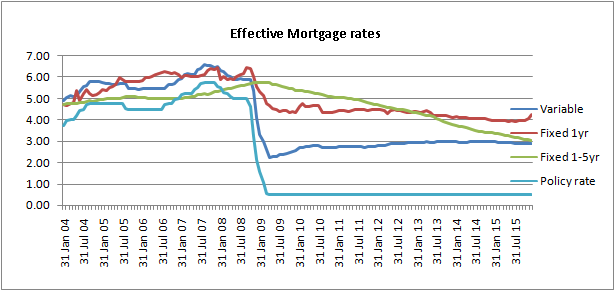
\includegraphics[width=0.9\textwidth]{mortgage}
	
\end{figure}

\begin{figure}[h!] 
\label{uk_corp_chart}
	\caption{Business lending rates in the UK} 
	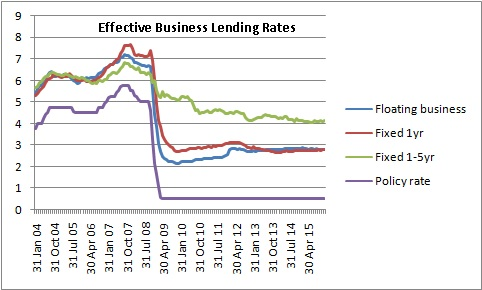
\includegraphics[width=0.9\textwidth]{busirate}
	
\end{figure}

We use the monthly data on effective interest rates (between January 2004 to January 2016)  for mortgage loans in the United Kingdom (for different terms of interest rate fixation) from Bank of England database.
As can be seen in figure below, the response of effective variable interest rate mortgages (to changes in the policy rate) is faster than the effective fixed interest mortgages (as expected).So also the response of the fixed interest mortgages decreases with the increase in the initial term of interest rate fixation.
The effective interest rates for longer term of initial interest rate fixation, change slowly as compared to the shorter term of initial interest rate fixation  because of the fixed nature of the interest rate for the respective term. The effective interest rate implies that a given portfolio of loans has a mix of older loans (which are being repaid over a period of time) which pay interest rate at the interest rates fixed in the past whereas the fresh loans pay interest at the current market rates (depending upon the interest rate pass through). As a result, even if the market interest rates change, the effective interest rates would not change immediately. They change slowly as the older loans are repaid and fresh loans are added to the loan portfolio over a period of time. The same can be observed in the graph for business interest rates

Interest rate stickiness arising due to fixed term loan contracts can vary across different sectors, depending upon the proportion of long term contracts in the portfolio. The following figure presents the effective lending rate for the overall portfolio of all fixed interest loans  (i.e.this includes different fixed term contracts) in case of business loans and mortgage loans. We find that the interest rate pass through is slower for the mortgage loan portfolio as compared to the business loan portfolio due to higher proportion of longer term fixed interest loan contracts.

\begin{figure}[h!] 
\label{uk_all_int_rates}
	\caption{Mortgage lending rates v/s Business lending rates in the UK} 
	\centering
	
	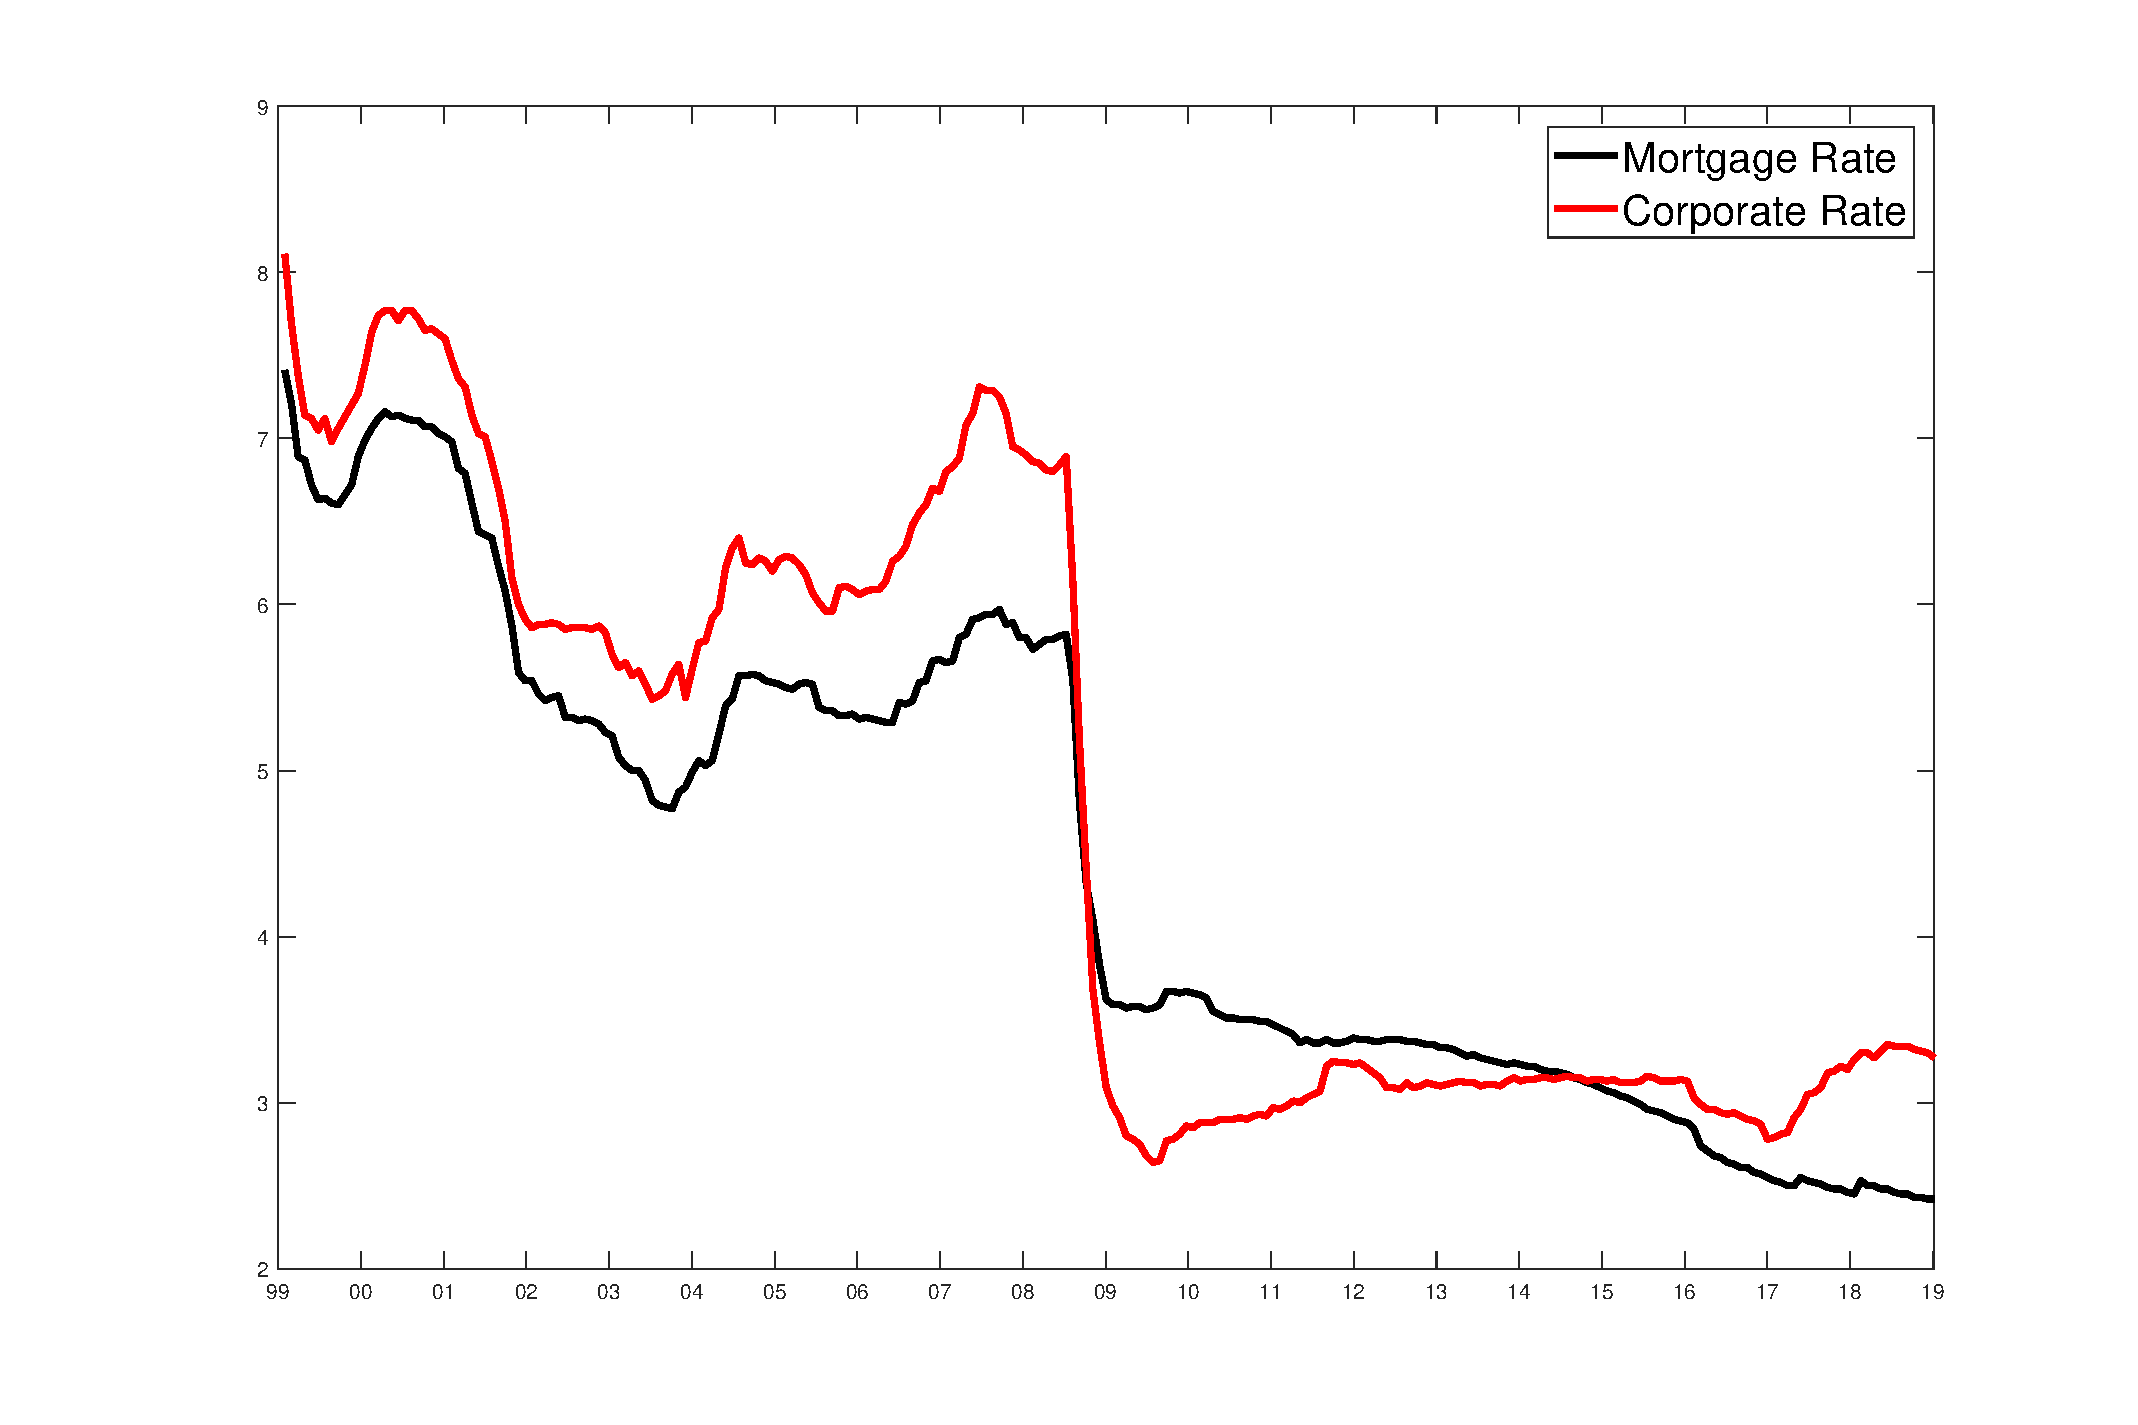
\includegraphics[width=0.9\textwidth]{int_rate_monthly_plot.pdf}
	
\end{figure}


\subsection{Econometric Methodology}

\hl{Is the data used in this section on \textbf{new lending} or the average of \textbf{all existing lending}? We need to make the former is used (that is also what we use in the model estimation section) } 

%summary: 
% floating rate--> 90% pass-through in the following month
% fixed 1-year--> 45% pass-through in the following month



As a first step to investigate the extent of sluggishness in the movement of interest rates, we attempt  to find out how lending rates change in response to change in central bank policy rate.Following the empirical literature on interest rate pass-through models ( \hl{some citations here would be nice} ) , we run a vector error correction model, where policy interest rates  are considered to be the most direct determinants of retail bank lending rates. We run the following vector error correction model based on Johansen (1991): 

\begin{equation}
{\Delta}R_{t}=\sum _{k=1}^{K }\delta_{k}{\Delta}R^m_{t-k}+\sum _{q=1}^{Q }\gamma_{q}{\Delta}i_{t-q}+\alpha (\mu+R^m_{t}-\beta i_{t})+u_{t}	
\end{equation}

Where $R_{t}$ is the effective lending rate (mortgage loans), $i_{t}$ is the Bank of England policy interest rate,coefficient $\beta$ is the long run equilibrium relationship between bank lending rate and policy rate and the coefficient $\alpha$ is the speed of adjustment of the lending rate to the long run equilibrium. The coefficients of the lags of the first difference of policy rate capture the short-run response of mortgage lending rates to the policy rate. We conduct this exercise for three different lending rates, variable interest rate, fixed interest for a term of up to 1 year and fixed interest rate for a term of 1 to 5 years. Results are summarized in the following table.


\begin {table}[H]
\label{regr_table_uk}
\caption {Regression of UK Bank lending rate on BOE policy rate} \label{tab:title} 
\begin{center}
	\begin{tabular}{||c c c c  ||} 
		\hline
		Regressor & Floating rate & Fixed $<$ 1 year& Fixed 1 to 5 year \\ [0.5ex] 
		\hline\hline
		$\i_{t}$ & $0.016^{***}$ & $0.0057$& $0.0025$ \\ 
		\hline
		$\Delta$ $\i_{t-1}$& $0.896^{***}$ & $0.435^{***}$& $0.018$  \\ 
		\hline
		 $\Delta$ $\i_{t-2}$&$0.016$ & -$0.293^{***}$& -$0.0158$\\
		
		\hline
	$\Delta$ $\i_{t-3}$	&  -$0.008$ & $0.242^{***}$& $0.0097$ \\
		\hline
		$\Delta$  $\i_{t-4}$&-$0.196^{***}$ &-$0.037$& $0.0054$ \\  
		\hline
		constant&$0.1366^{***}$ & - & -\\ 
			
			\hline
		
		\hline
		
	\end{tabular}

\end{center}

\end {table}
\footnotetext{*** is 1 per cent, ** is 5 per cent and * is 10 per cent level of significance }



In case of floating interest rate loans, the response on impact is very low. However,around 90 percent of the pass through takes place in the following month.

The above table highlights that the response of floating interest rate (as depicted by coefficient $\gamma_{q}$ ( \hl{what is the corresponding $\gamma_q$ in the table? Is the constant equivalent to $\alpha * \mu$? Notation on deltas should be also be consistent in the table and regression model maybe? }))  on the central bank policy rate is higher than the response of 1 year fixed rate loans, which in turn is higher than the response of the 1 to 5 year fixed rate loans.

 In case of fixed term of up to 1 year, the response on impact is very low (less than 0.01 percentage point) and around 45 per cent of the pass through takes place in the following month. 

The pass through for the 1 to 5 year fixed term loans is very low.  However,there exists a long term co-integration relationship between the two interest rates. \hl{do we interpret the table as follows: there is no significant pass-through in the following 4 months on 1-5 year fixed-term loans because none of the coefficients are significant?  }
\hl{relatedly: does the negative term on $\beta_{t-2}$ on fixed<1year loans mean the pass-through works in the opposite direction in that month? Summing up all the coefficients, can we claim the pass-through in the following 4 months in only 45 \%? }

For the fixed rate loans, the sum of short run coefficients is less than 1 suggesting an incomplete pass through of policy interest rate.

Thus, the pass through to the fixed interest loans is not only sluggish but also incomplete, whereas the pass through to variable interest loans is faster and almost complete.However, in all the cases including floating interest rate, the response of lending rate on impact is very low (less than 2 percent) \hl{what is "all cases" referring to here? Isn't there only regression here with the floating rate?}.

The fact that  floating interest rates adjust faster than the fixed term interest rates,implies that the existence of fixed rate contract is an important source of interest rate sluggishness. So also,the pass through of interest rate changes on impact (i.e. the speed of adjustment) is very small implies that other sources of stickiness such as switching costs, menu costs, market structure/competition, regulation could also be relevant.




 
\section{Model Overview}
\hl{add the shock explanations here}An
Our model closely follows Clerc et. al. (2015), which augments the baseline model of Bernarke, Gilchrist and Gertler (1999) with a detailed banking sector and different types of default on households, corporates and banks to determine the optimal capital adequecy ratio (CAR) for the banking sector, as well as to analyze the macroeconomic implications of bank capital structure under different shocks. 

The BGG framework assumes that interest rates charged by the banks are state contingent. This implies that higher interest rates charged on non-defaulters are sufficient to meet the losses arising from defaulters. This means that banks always make a risk-free return on their investments, which makes the capital structure of the bank irrelevant in the original BGG framework.

Clerc et. al. (2015) departs from the BGG framework by assuming a non-contingent lending rate, which implies that in the event of defaults by borrowers, banks may also suffer losses. Therefore, with costly state verification of borrowers, defaults are costly and entail a dead-weight loss for the economy, which necessitates a role for bank capital. They further assume that investor wealth is scarce and hence cost of equity capital is higher than debt funding. This implies that although bank capital is necessary to avoid higher default rates, it is also expensive at the same time, thus creating a trade-off for holding capital. 

Our model deviates from Clerc et. al. (2015) in several important ways. On the banking side, we introduce staggered interest rates à la Calvo (1983) to capture the sluggishness of mortgage and corporate lending rates, which is motivated by the empirical evidence shown in Section 3. Further, we endogenize the bank's capital level by allowing it to be determined in equilibrium through the bank's decision problem. Accordingly, the bank maximizes over its lending rates to households and businesses subject to interest rate sluggishness. The minimum and sectoral capital requirements are introduced as penalty costs on the bank's decision problem, which creates a precautionary motive for the bank to hold a capital level higher than the minimum required. This is a realistic setup since banks typically maintain capital buffers to ensure they do not breach the regulatory minimum. This differs from Clerc et. al. (2015), which assumes that banks always hold the minimum capital requirement. 


On the household side, we introduce a Loan to Value (LTV) limit, which is a key feature of the mortgage lending market. The LTV limit is qualitatively similar to an exogenous collateral constraint as in Iacoviello. We further introduce a similar LTV limit on businesses, although we do not evaluate the impact of this since the Financial Policy Committee (FPC) in the U.K. does not have such a regulatory tool \hl{is this a correct way of phrasing it?}. 


Other key distortions and frictions in the model follow Clerc et. al. (2015). Accordingly, both the bank and borrowers in the model are subject to limited liability. The limited liability of banks, along with the presence of deposit insurance implies that banks have an incentive to over-borrow and thereby over-lend, since they do not fully internatilize the costs of default suffered by the deposit insurance agency and the economy as a whole. As such, regulatory capital is a means to restrict the use of excessive bank leverage. The model further features costly state verification, which implies that the use of leverage is more expensive and that defaults are costly. 


Key agents in the economy are patient and impatient households, entrepreneurs, banks, a deposit insurance agency, housing, \& capital and final goods producers. Figure ?? provides an overview of all economic agents. Below we provide the maximization problem for each agent type. The associated first-order conditions can be found in the Appendix. 


\begin{figure}[H]
	\label{model_overview_chart}
	%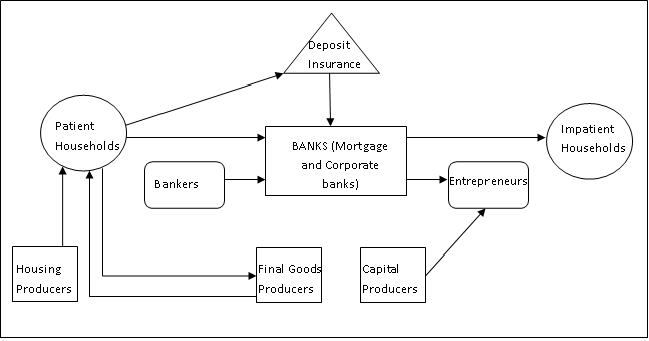
\includegraphics[width=0.9\textwidth]{DIAGRAM1}
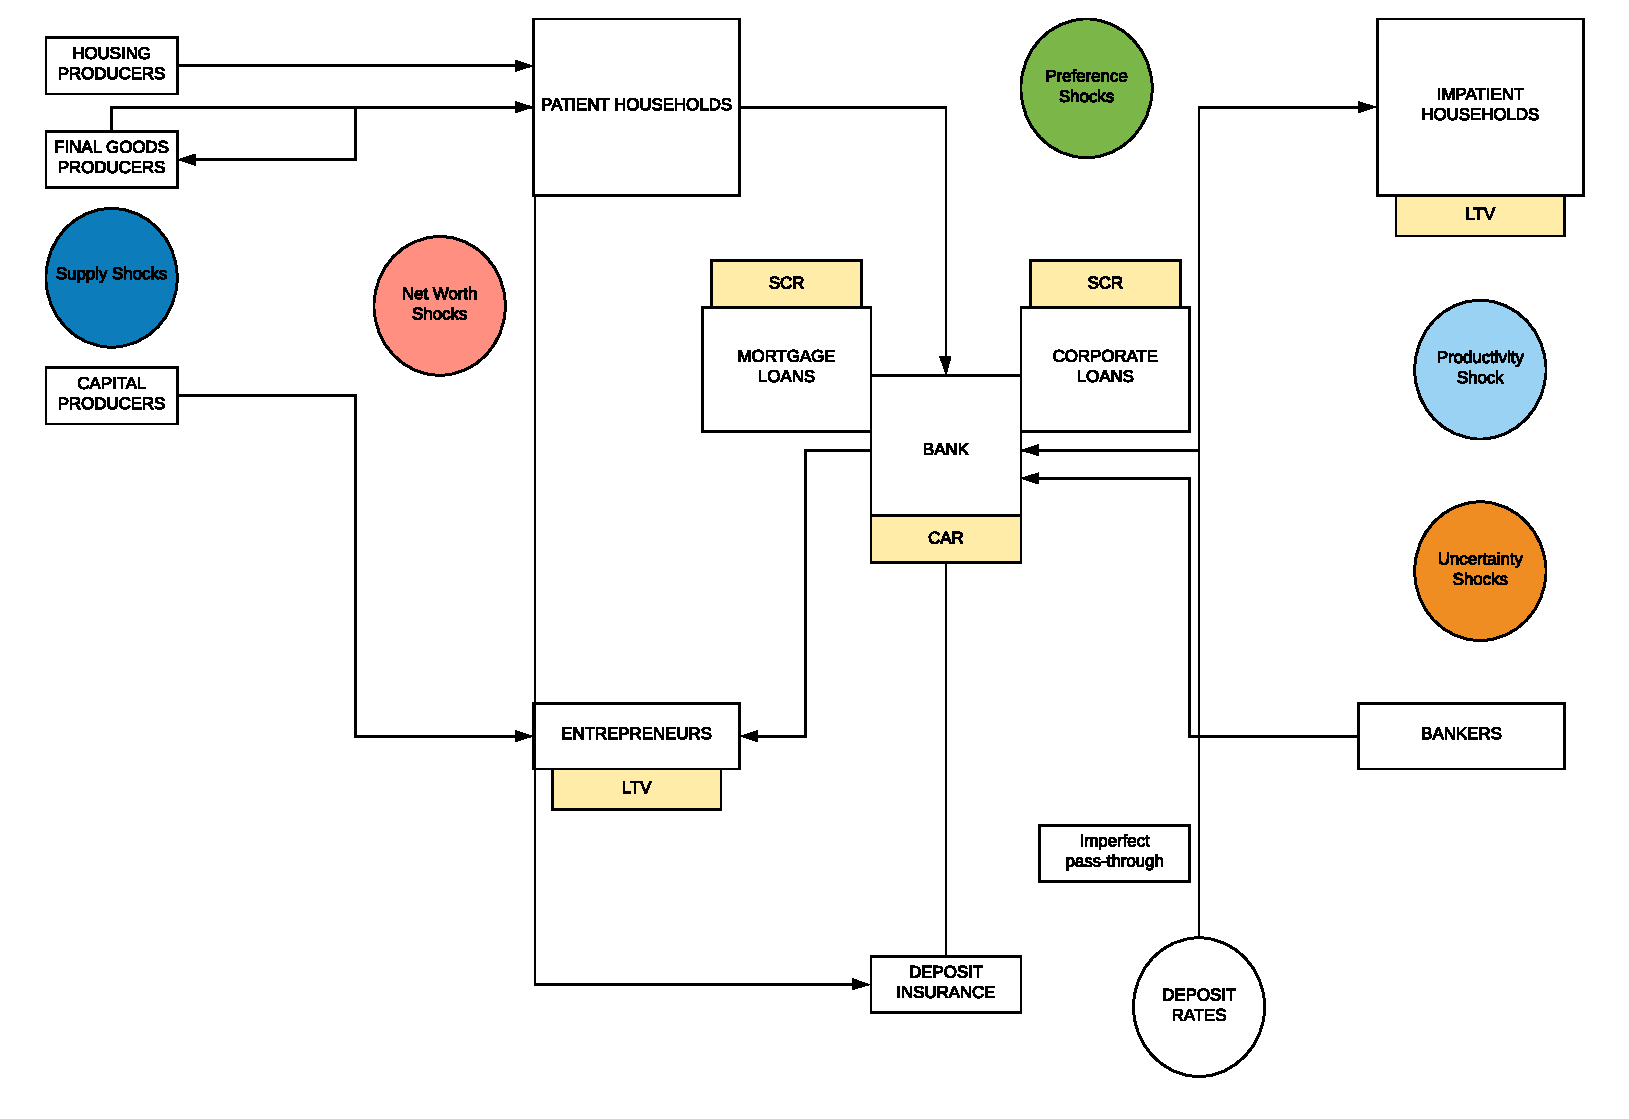
\includegraphics[width=0.9\textwidth]{3d_model_overview.pdf}
\end{figure}

\textbf{Households:} there are two types of households, patient and impatient, with patient households having a higher discount factor as in Iacoviello (2015).Both patient and impatient households have concave utility functions and derive utility from consuming goods, housing and leisure. The individual households are a part of a representative dynasty,which provides perfect risk sharing within the group. Thus, all individual households within the type are identical.Even if the individuals face idiosyncratic shocks, they are perfectly insured within their dynasty and hence consume and save/borrow identically.Both households supply labour in a competitive labour market.

\textbf{Patient households}:
In equilibrium, patient households are savers that supply deposits with the bank and buy housing with their own funding.
Patient households derive utility from consumption goods and housing, while deriving disutility from labour. Hence they maximize the following objective function:
\begin{equation}
\max_{c^s_t,L^s_t,D_{t},H^s_t}E_t\sum _{t=0}^{\infty } \beta_{s}^t [log(c^s_t)+vlog(H^s_t)-\frac{(L^s_t)^{1+\eta}}{1+\eta} ]
\end{equation}
subject to the following budget constraint:
\begin{equation}
c^s_t+q^H_{t}H^s_{t} +{D_{t}}=w_{t}L^s_{t}+q^H_{t}H^s_{t-1}(1-\delta)+{D_{t-1}}R^D_{t}+\pi_{t}
\end{equation}

The term $\pi_{t}$ includes profits of final goods producing firms and investment/housing production firms (which are owned by patient households), dividends from entrepreneurs and lumpsum transfers from deposit insurance agency. 






\textbf{Impatient households:}
Impatient households borrow from banks using their houses as collateral as in Bernanke, Gertler \& Gilchrist (1999) . These mortgage loans are made on a limited liability non-recourse basis,  implying that individual households default whenever the value of the house is lower than the outstanding mortgage loans.The value of the house depends both on aggregate shocks (which affect house prices) as well as an idiosyncratic shock which determines whether an individual borrower defaults. In equilibrium, borrowers with an idiosyncratic shock below a certain threshold default.In the case of default, the bank takes possession of the houses in which case it is subject to state verification costs.

The borrowing is subject to LTV (Loan to value) limit set by the regulator. It is similar to a borrowing/collateral constraint as in Kiyotaki \& Moore (1997).

The objective function of the impatient households is the same as that of the patient households except for the discounting factor:
\begin{equation}
\max_{c^m_t,B^m_t,L_{t},H^m_t}E_t\sum _{t=0}^{\infty } \beta^t_{m} [log(c^m_t)+vlog(H^m_t)-\frac{(L^m_t)^{1+\eta}}{1+\eta} ]
\end{equation}

The budget constraint of impatient households reflects their borrowings under limited liability:
\begin{equation}
c^m_t+q^H_{t}H^m_{t} -B^m_{t}=w_{t}L^m_{t}+\int_{\bar{\omega^m_{t} }}^\infty  \left(\omega^m_{t} q^H_{t} H^m_{t-1} (1-\delta)B^m_{t-1}R_{t-1}\right) \, dF\omega^m_{t} + P_{t}
\end{equation}

The term under the integral reflects the limited liability of the borrowers as they default on their loans when the idiosyncratic shock $\omega^m_{t}$ is below the threshold level of $\bar{\omega^m}_t$. 

The default decision by the borrowers is given by:
\begin{equation}
{{\omega^m_{t} }}q^H_{t} H^m_{t-1}(1-\delta) <= B^m_{t-1}R^m_{t-1}
\end{equation}

The threshold level of $\bar{\omega^m}_t$ satisfies:
\begin{equation}
\bar{\omega^m}_t q^H_{t} H^m_{t-1}(1-\delta) = B^m_{t-1}R^m_{t-1}
\end{equation}


The LTV limit (or the borrowing constraint) is given by:
\begin{equation}
[B^m_{t}-(1-rp)B^m_{t-1}]R_{t} <=\epsilon_{t} E_t[q^H_{t+1} [H^m_t-H^m_{t-1}(1-\delta)]]
\end{equation}

where rp is the loan repayment rate and $\epsilon_{t}$ is the LTV limit.

The limit always binds in the steady state and it's neighborhood.





\textbf{Entrepreneurs:}
Entrepreneurs are risk neutral agents who own and maintain the stock of physical capital. They rent  capital to the final goods producing firms. Entrepreneurs derive utility from transferring part of their wealth to the saving dynasty (paying dividends) and retaining the rest for the next period (retained earnings). Entrepreneurs invest in capital goods and finance their investment by means of their own funds (net worth) and borrowings from banks. Similar to mortgage loans, these are limited liability non-recourse loans and hence subject to default by individual entrepreneurs in the event of value of assets falling below the outstanding loans.The value of the capital depends both on aggregate shocks (which affect house prices) as well as an idiosyncratic shock which determines whether an individual entrepreneur defaults. In equilibrium, borrowers with an idiosyncratic shock below a certain threshold default.  As in the case of households, assets are seized by banks and subject to costly state verification costs. 

\begin{equation}
\max_{K_t,B^e_t}E_t(W^e_{t+1})
\end{equation}	


\begin{equation}
W^e_{t+1}=max[\omega^e_{t+1}(r^k_{t+1}+(1-\delta)q^K_{t+1}K_{t})-R^F_{t}b^e_{t},0]
\end{equation}


The default decision of the entrepreneurs is given by:
\begin{equation}
{{\omega^e_{t} }}q^H_{t} K_{t-1}(1-\delta) <= K_{t-1}R^f_{t-1}
\end{equation}

The threshold level of $\bar{\omega^m}_t$ satisfies:
\begin{equation}
\bar{\omega^e}_t q^K_{t} K^m_{t-1}(1-\delta) = B^e_{t-1}R^f_{t-1}
\end{equation}
As borrowing is subject to LTV limit as follows:

\begin{equation}
[B^e_t-B^e_{t-1}(1-rp)]R^f_{t} =\epsilon_{t} E_t[q^F_{t+1} [K_t-K_{t-1}(1-\delta)]]
\end{equation}
Dividend rule:

A fixed proportion of wealth $\chi^e$ is paid out as dividends. This simple dividend paying rule for the entrepreneurs is given by:
\begin{equation}
c^e_t=\chi^e W^e_t
\end{equation}
As a result the retained earnings by the entrepreneurs is given by:
\begin{equation}
n^e_t=(1-\chi^e) W^e_t
\end{equation}

The balance sheet identity of the entrepreneurs is :
\begin{equation}
n^e_t+B^e_t=q^K_t K_t
\end{equation}

\textbf{Banks:} \\
\hl{-4.18 through 4.21, and then 4.23 through 4.25 seem like entirely different things. I do not think we have the former in the model? Could that be the older version?\\
-"marginal cost" needs a better phrasing } \\

Banks are financial intermediaries who channel savings from the savers to the borrowers.On the asset side of the banks, there are loans to households (mortgage lending) and entrepreneurs (business lending) respectively. As described earlier, these loans may default depending on aggregate state shocks and idiosyncratic borrower shocks in which case the banks seize the assets subject to state verification costs (these can also be viewed as bankruptcy costs).

On the liability side, there are deposits held by the patient households and equity capital held by the bankers. Deposits are insured by the Deposit Insurance agency. There is a capital adequacy requirement set by the regulator which along with a penalty cost function, which determines the amount of equity capital held by the bankers.

The key feature of the model is that banks may also default depending upon the performance of their loan portfolios (aggregate shocks) and idiosyncratic shocks (on similar lines as  the borrowers). The banks face an idiosyncratic shock to their returns on loans.Thus, in equilibrium, a fraction of banks below a certain threshold of the idiosyncratic shock level default. In case of default, the bank loan assets are also subject to possession  by the deposit insurance agency and costly state verification.

The banks' balance sheet identity is as follows:
\begin{equation}
n^b_{t}+D_{t}=B^m_{t}+B^e_{t}
\end{equation}

The maximization problem of the bank is given by:

\begin{equation}
\resizebox{1\textwidth}{!}{$
	\max_{R^{mi}_t,R^{fi}_t}E_t\sum _{t=0}^{\infty }\xi^t\beta_{s}^t [\{(1-G^H_{t+1}) (\widetilde{R^{mi}_{t}})(B^{mi}_{t})+(1-G^F_{t+1})\widetilde{R^{fi}_{t}}B^{ei}_{t}\}-(1-F^){R^D_{t}}D_{t}+Penalty cost]$}
\end{equation}



\begin{equation}
\widetilde{R^{mi}_{t}}=(1-E_tF^m_{t+1})R^{mi}_t+E_tG^m_{t+1}(1 - \mu^m)( R^{mi}_t/E_t\bar{\omega}^m_{t+1})
\end{equation}
\begin{equation}
\widetilde{R^{fi}_{t}}=(1-E_tF^e_{t+1})R^{fi}_t+E_tG^e_{t+1}(1 - \mu^e)( R^{fi}_t/E_t\bar{\omega}^e_{t+1})
\end{equation}

The demand for Loans is given by:
\begin{equation}
B^{mi}_t=(\frac{R^{mi}_t}{R^{m}_t})^{-\tau} B^{m}_t
\end{equation}

\begin{equation}
B^{ei}_t=(\frac{R^{fi}_t}{R^{f}_t})^{-\tau} B^{e}_t
\end{equation}



$R^{mi}$ and $R^{fi}$ are the rates of interest that the bank would charge in the absence of interest rate sluggishness. $\tau$ is the elasticity of substitution and determines the market power of the bank, while $\mu$ represent the bankruptcy cost of households and firms respectively. \hl{is this paragraph correct?}

\textbf{Penalty cost function:}
Penalty costs are modeled as a non pecuniary gain in utility if the capital adequacy ratio is higher than the minimum capital requirement and a non pecuniary cost if the capital adequacy ratio is lower than the minimum capital requirement.

\begin{equation}
Penalty cost_t=\nu^b \frac{[\frac{\phi^b_t}{\bar{\varphi_t}}]^{1-\sigma}-1}{{1-\sigma}}
\end{equation}

The above functional form,based on Nukhwoon \& Tsomocos (2018) builds in a non-linearity in the penalty costs.The marginal gains of having excess capital are decreasing whereas the marginal costs of having a shortfall in capital are increasing, whenever $\sigma$ is greater than 1. This creates an incentive for banks to maintain capital at a higher level as compared to the minimum regulatory requirement. In reality, we find that banks do maintain capital buffer over what is the minimum required.The parameter $\nu^b$ determines the weight attached to this penalty costs.

\textbf{Staggered interest rates:}
Although, interest rate stickiness can be attributed to various reasons such as switching costs,menu costs, market structure, regulation etc.,we find the one of the main sources of interest rate sluggishness is the existence of fixed interest loans.

We introduce interest rate stickiness in a broader sense by modeling it as in Calvo (1983). This approach also has the benefit that it includes all possible sources of interest rate sluggishness in a reduced form (including the effect of long term fixed interest loans).It is assumed that only a 1-$\xi$ proportion of banks are able to change their interest rates in a given period, whereas the remaining $\xi$ proportion of banks are not able to change their interest rate. This staggered interest rate setting implies that the composite interest rate in the economy is an average of the current interest rate charged by the fraction of banks who can change the interest rate and the previous period interest rate.
To micro-found the staggered interest rate setting, we assume that there is imperfect competition in the banking sector. Banks offer differentiated loan products as in Gerali et al (2010) and are able to set their interest rate in the monopolistically competitive loan market.The borrowers takes a composite loan product comprising of all the aforesaid differentiated banking services.The composite interest rate paid by the borrowers is thus staggered on account of the Calco friction.In short,we extend the New Keynesian approach to goods market to the loan markets so as to generate interest rate stickiness. 

The FOCs for the interest rates are as follows.The FOC is similar to the FOC for price in a standard New Keynesian model with goods price stickiness:

\begin{equation}
R^{mi}_t=\frac{\tau}{\tau-1}\frac{E_t\sum _{t=0}^{\infty }\xi^t\beta_{s}^t MC_t}{E_t\sum _{t=0}^{\infty }\xi^t\beta_{s}^t rm_t}
\end{equation}
\begin{equation}
R^{fi}_t=\frac{\tau}{\tau-1}\frac{E_t\sum _{t=0}^{\infty }\xi^t\beta_{s}^t MC_t}{E_t\sum _{t=0}^{\infty }\xi^t\beta_{s}^t rf_t}
\end{equation}

\begin{equation}
MC_t=\lambda_{st+1}[(1-bankdef.prob)R_{Dt}+\frac{\nu^b(\phi^b_t/{\bar{\varphi_t}})^{(1-\sigma)}}{(B^{mi}_t+B^{ei}_t)}](R^m_t)^\tau B^m_t
\end{equation}

As in the New Keynesian model with price stickiness, the interest rate charged by banks is a function of present discounted value (with the stickiness parameter) of present and future marginal cost times the mark up. The marginal cost includes the interest rate paid on deposits (in a competitive deposit market) and the penalty cost associated with the deviation from the regulatory capital requirement. The only difference from the standard New Keynesian version is the presence of borrower and bank defaults in the interest FOC for interest rate equation

\textbf{Deposit Insurance Agency:}
The deposit insurance agency insures the deposits. The assets of the defaulting banks are taken over by the agency and is subject to bankruptcy costs.The difference between the amount of deposits and the value of assets realized assets is recovered by the charging a lumpsum tax on households. 


\textbf{Final goods producing Firms:} 
There is a unit mass of perfectly competitive firms which combine capital and labour to produce the consumption good which is the numeraire.The firms rent capital from entrepreneurs. The firms are owned by patient households. They produce the final goods using a standard Cobb Douglas technology.

\begin{equation}
Y_{t}=A_{t} K^{\alpha}_{t-1}L^{1-\alpha}_{t}
\end{equation}

\textbf{Capital goods and Housing production:}
These are competitive firms which buy finished goods and produce capital goods /housing subject to quadratic adjustment costs.These firms produce new units of capital and housing using consumption goods which are then sold to entrepreneurs and households,respectively, at prices qK and qH. They represent the supply side of the capital goods/housing and pin down the equilibrium asset prices.These firms are also owned by the patient households.



\subsection*{Exogenous Shocks}

The model is equipped with 13 exogenous shocks modelled as AR(1) processes across different sectors. On the housing side, we have a housing depreciation shock $Hd_t$, which directly affects the return on housing stock for both types of households. A positive shock therefore directly translates into a reduced stock of housing owned by households, and therefore a lower rate of return on housing. We further have two preference shocks on consumption $EC_t$ and housing $J_t$, which affect the preference of both household types. An adverse preference shock translates into less purchasing of a given commodity type, therefore these shocks can be equivalently interpreted as risk aversion shocks to the given commodity type. We further have an uncertainty shock $Sm_t$ on impatient households, which affects the volatility of their default rate. A larger volatility implies a larger number of agents falling below their default threshold, and therefore a larger risk shock correspond to higher default rates. 

On the corporate side, we have a capital depreciation shock $Hk_t$ and an uncertainty shock $Se_t$ on entrepreneurs, which have an analogous meaning to the shocks on households. We further have a net worth shock $We_t$ on the firm value. Since the business is owned by the patient households, since shocks correspond to income or budget constraint shocks for patient households. 

On the bank side, we have an uncertainty and a net worth shock, $Sb_t$ and $Wb_t$, that have similar interpretations as their household and business counterparts. We further have a bank capital shock $ECAB_t$ that directly affects the amount of capital that the bank holds. In the absence of inflation and monetary policy, this shock plays a dominant role in driving deposit and lending rate fluctuations and can be interpreted as a quasi monetary policy shock. Finally, there are two mark-up shocks $EM^H_t$ and $EM^F_t$ that affect the cost of mortgage and corporate lending, which help to introduce a wedge between deposit and lending rates. 

Finally, we have a productivity shock $A_t$ that directly affects aggregate output. 



%This shock play a dominant role in driving deposit and lending rate fluctuations. Therefore, in the absence of inflation and monetary policy in our model, this shock 


%Household side--> housing depreciation, uncertainty shock on impatient households, 2 preference shocks on consumption and housing. 


%Business side--> capital depreciation, risk shock on entrepreneurs, net worth shock


%Bank side--> bank capital shock, 2 markup shocks on lending rates, risk shock on the bank, net worth shock


%aggregate side--> productivity, 

%The model is equipped with 13 shocks: \\
%-Productivity shock on output, $A_t$\\
%-Housing and capital depreciation shocks, $Hd_t$ and $Hk_t$. These are shocks directly affecting the depreciation rates of housing and capital stocks. Therefore a positive shock directly translates into a reduced stock of housing or capital owned by households, and therefore a lower rate of return on housing or capital. \\
%-Risk (uncertainty) shocks on Entrepreneurs $Se_t$, impatient households $Sm_t$ and the bank $SB_t$. These shocks affect the volatility of default rates for the associated agents. In other words, these shocks are changes in the volatility of cross-sectional idiosyncratic uncertainty. A larger volatility implies a larger number of agents falling below their default threshold, therefore larger risk shocks directly translate into higher default rates.  \\
%-Net worth shocks on corporates and the bank, $Wb_t$ and $We_t$: since the bank and the business are owned by patient households, these shocks translate into budget constraint shocks on the patient households. \\
%-Household preference shocks $J_t$ and $EC_t$. These are shocks on the household and consumption preference of both types of households. A negative household or consumption shock means less purchasing of that commodity type, therefore they can be equivalently interpreted as risk aversion shocks to the given commodity type. \\
%-Bank capital shock $CAB_t$: this is a shock directly affecting the capital ratio of the bank. In the absence of a monetary policy authority, these shocks can be interpreted as a proxy for monetary policy shocks. \\
%-Markup, or cost-push shocks $H_{markup,t}$ and $F_{markup,t}$: these are shocks on the mortgage and corporate rate that the bank would like to set. An increase in either shock can be interpreted as an external factor that pushes up the bank's cost of lending, which results in an increase in the rate that the would set in the absence of sluggishness. As such, these are shocks to the wedge interest rate wedge driven by stickiness.

\section*{Estimation}



\subsection*{Measurement equations} 

We use 10 quarterly variables from U.K. over the period $1998Q1-2016Q4$ for the following key variables: 

\begin{itemize}
\item Output growth:\\
$\Delta Y_t^{obs}=\gamma_Y+ Y_t-Y_{t-1}$

\item Wage growth:\\
$\Delta W_t^{obs}=\gamma_W+ W_t-W_{t-1}$

\item Investment growth:\\
$\Delta I_t^{obs}=\gamma_I+ I_t-I_{t-1}$

\item Consumption growth:\\
$\Delta C_t^{obs}=\gamma_C+ C_t-C_{t-1}$

\item Mortgage lending rate:\\
${R^{H,t}}^{obs}=100(\bar{R^H}-1) + R^m_t$
\item Business lending rate:\\
${R^{m,t}}^{obs}=100(\bar{R^m}-1) + R^m_t$

\item Deposit rate: \\
${R^{D,t}}^{obs}=100(\bar{R^D}-1) + R^D_t$


\item House price growth rate: \\
$\Delta {q^{H,t}}^{obs} =\gamma_{\Delta q^H} + q^H_t - q^H_{t-1}$
\item Business lending growth rate:\\
$\Delta {b_{e,t}}^{obs}=\gamma_{\Delta b_e}+  b^e_t - b^e_{t-1} $

\item Mortgage lending growth rate:\\
$\Delta {b_{m,t}}^{obs}=\gamma_{\Delta b_m}+  b^m_t - b^m_{t-1} $

\end{itemize}

where $\gamma_Y,\gamma_W,\gamma_I,\gamma_C,\gamma_{\Delta q^H} $ and $\gamma_{\Delta b}$ are obtained by demeaning the series prior to estimation, since our model does not feature steady-state growth. $\bar{R^H}, \bar{R^m}$ and $\bar{R^D}$\footnote{We assume that the deposit rates are equivalent to the official Bank Rate in our estimation exercise since there is no monetary policy in our model. In the presence of monetary policy, an alternative would be to introduce another layer of sluggishness from the Bank Rate to deposit rates. However, Pariès et. al. (2010) find little evidence for the importance of this channel based on EU data.} denote the gross lending and deposit rates at the steady-state of the model.  

\subsection*{Calibrated parameters and Prior Distributions }

Prior to estimation, we fix a number of parameters by either following conventional values used in the literature or to generate steady-state values consistent with U.K. data. Parameters relating to default costs are based on Mendicino et. al. (2015): the depositor cost of bank default $\gamma$ is fixed at $0.1$. The bankruptcy cost of households, businesses and banks $\mu_m, \mu_e$ and $\mu_B$ are set to a common value of $0.3$. The discount factor for patient households is $0.995$. 


For some parameters, we use standard values following convention in the literature. Accordingly, capital share in production is set to $0.3$, while the Frisch elasticity of labor $\eta$ is $1$. The labor preference parameters for both types of households $\varphi_s$ and $\varphi_m$ are normalized to $1$ since they mainly scale the size of the economy. The parameters $a_s$ and $a_b$ are set to $0.5$, which determine the share of total default costs paid by saving and borrowing households respectively. 


Some parameters are closely linked with the steady-state of the economy. We use these parameters to generate plausible ratios for some of the key variables. The housing preference parameters for both types of households, $v_s$ and $v_m$, as well as business and bank dividend payout parameters, $\chi_e$ and $\chi_b$, are used to generate plausible business and mortgage lending to aggregate output ratios.  Accordingly, we set $v_s=0.25$ and $v_m=0.5$, while the divident payouts are set to $\chi_e=0.1$ and $\chi_b=0.15$. These generate lending ratios of $133 \%$ and $86 \%$ for corporate and mortgage lending to output respectively, which are reasonably close to the historical means of the corresponding U.K. ratios over the estimation period, which are $118 \%$ and $81 \%$ respectively. At the given values, mortgage lending constitutes $38 \%$ of total lending in steady-state. Similarly, we set the housing and capital depreciation rates to $\delta_H=0.01$ and $\delta_K=0.04$, which yields an investment to output ratio of $0.12 \%$, which is close to the historical mean of $0.17 \%$ for the U.K. economy over this period \hl{where did I take these ratios from?}. 

The parameters determining market power of the bank, $\tau_m$ and $\tau_F$ are both set to 40, whereas the hyperparameters in the cost function are set to $\psi_b=5$ and $\nu=0.5$. 

Parameters relating to macroprudential regulation are fixed in our benchmark estimations. Accordingly, for minumum capital requirements, we use a benchmark value of $\phi_H=\phi_F=0.11$ for both sectors, which is close to the historical minimum capital requirements for U.K. over this period. We further assume there is no CCyB in place in our benchmark estimations.  Similarly, the LTV limit for both households and businesses is assumed to be fixed in our benchmark estimation, which is set to $0.86$, close to the historical average over this period for the U.K. economy. \hl{specify which periods and which values these historical averages correspond to}. 


The remaining 35 parameters are estimated using Bayesian likelihood methods to match the data. Table \ref{prior_dist_table} provides a summary of of the prior distributions used in our estimation: for the AR(1) coefficients of all exogenous shocks, we use a standard Beta distribution with mean $0.5$ and standard deviation $0.2$ following Smets-Wouters (2007) \hl{add to citations}. The standard deviations of all exogenous shocks are assigned a diffuse uniform prior over the interval $[0,10]$. The volatility of i.i.d. shocks on households, businesses and banks follow a common Inverted Gamma distribution with mean $0.1$ and standard deviation $2$: we choose to use more informative priors for these parameters since both aggregate and i.i.d shocks mainly relate to the level of default rates in a first-order approximation, hence estimating both sets of parameters with uninformative priors may lead to identification issues. For the cost adjustment parameters $\psi_i$ and $\psi_h$, we assume a conventional normal distribution with a mean of $5$ and standard deviation $2$, which is a wider and less informative prior than previous literature (\hl{see e.g. Smets-Wouters which assumes ~N(4,1.5), check also what is assumed in the Compass model (both for this variable and other variables in general that may be related)}).Finally, for the Calvo parameters on interest rates, we follow Pariès et. al. (2010) and assume a Beta distribution with mean $0.5$ and standard deviation $0.2$. This is similar to previously assumed priors for Calvo price setting on prices and wages, which typically follows similar Beta distributions. 

We notice that the steady state is very sensitive to the remaining 4 parameters: habit formation $\lambda$, repayment rates for households $rp$ and businesses $rpe$, and the discount factor of impatient households $\beta_m$. For these parameters, the likelihood function is also very irregular and we observe large jumps in the objective function for small parameter changes, which makes the computation of standard errors and posterior distributions around these variables very hard with conventional methods. For these parameters, we therefore use the following approach: we compute the point estimates for the candidate density (i.e. posterior mode) without computing the standard errors. These 4 parameters are then fixed at their point estimates and are exluded in the posterior MCMC draws, i.e. we compute the posterior distributions of the remaining 31 parameters conditional on the point estimates of these 4 parameters\footnote{The posterior distribution of the remaining 31 parameters are computed using 4 parallel MCMCs, each with 200000 draws where the first half of each chain is discarded as the burn-in sample. The scaling coefficient of the parameter covariance matrix is adjusted to obtain an acceptance ratio of around $35\%$ in each case.}.

 
\begin{table}[H]
\caption{Prior Distributions}
\label{prior_dist_table}
\begin{tabular}{l|l|l|l}
Parameter & Prior &  &  \\
\hline
\hline
 & Dist & Mean & Variance \\
 \hline
\hline
$\epsilon_{Hd}$ & Uniform & 10 & 5.77 \\
$\epsilon_{Hk}$ & Uniform & 10 & 5.77 \\
$\epsilon_{A}$ & Uniform & 10 & 5.77 \\
$\epsilon_{J}$ & Uniform & 10 & 5.77 \\
$\epsilon_{Se}$ & Uniform & 10 & 5.77 \\
$\epsilon_{Sm}$ & Uniform & 10 & 5.77 \\
$\epsilon_{SB}$ & Uniform & 10 & 5.77 \\
$\epsilon_{We}$ & Uniform & 10 & 5.77 \\
$\epsilon_{markup_m}$ & Uniform & 10 & 5.77 \\
$\epsilon_{markup_e}$ & Uniform & 10 & 5.77 \\
$\epsilon_{EC}$ & Uniform & 10 & 5.77 \\
$\epsilon_{ECAB}$ & Uniform & 10 & 5.77 \\
$\sigma_e$ & Inv. Gamma & 2 & 0.1 \\
$\sigma_m$ & Inv. Gamma & 2 & 0.1 \\
$\sigma_B$ & Inv. Gamma & 2 & 0.1 \\
$\psi_i$ & Normal & 5 & 2 \\
$\psi_h$ & Normal & 5 & 2 \\
$\zeta_m$ & Beta & 0.5 & 0.2 \\
$\zeta_e$ & Beta & 0.5 & 0.2 \\
$\rho_{Hd}$ & Beta & 0.5 & 0.2 \\
$\rho_{Hk}$ & Beta & 0.5 & 0.2 \\
$\rho_{A}$ & Beta & 0.5 & 0.2 \\
$\rho_{J}$ & Beta & 0.5 & 0.2 \\
$\rho_{Se}$ & Beta & 0.5 & 0.2 \\
$\rho_{Sm}$ & Beta & 0.5 & 0.2 \\
$\rho_{SB}$ & Beta & 0.5 & 0.2 \\
$\rho_{We}$ & Beta & 0.5 & 0.2 \\
$\rho_{markup_m}$ & Beta & 0.5 & 0.2 \\
$\rho_{markup_e}$ & Beta & 0.5 & 0.2 \\
$\rho_{EC}$ & Beta & 0.5 & 0.2 \\
$\rho_{ECAB}$ & Beta & 0.5 & 0.2 \\
$\beta_m$ 	  &   Beta   &  0.98   & 0.01    \\
$\lambda$ 	  &  Beta    &   0.5  &   0.2  \\
$rp$ 	  &   Beta   &   0.05  &   0.025  \\
$rpe$ 	  &   Beta   &   0.05  &   0.025  \\
\end{tabular}
\end{table}

\section*{Posterior Estimates \& Distributions}

Table \ref{posterior_dist_table} reports the point estimates as well as the 95\% HPD intervals of all estimated parameters.

Of particular interest are Calvo parameters, for which the posterior distributions are along with the posterior mean and mode are shown in Figure \ref{posterior_dist_calvo}. We find a Calvo probability of 44.7 \% for corporate rates, whereas the probability for mortgage rates is 69.1 \%. This means banks are able to reset the interest rates on corporate loans once every 1.81 quarters or 5.42 months, while it takes much longer to reset the interest rates on mortgage loans with an average of 3.24 quarters or 9.71 months. The 95 \% confidence intervals are $[4.73,5.93]$ months for corporate rates and $[8.21,11.1]$ months for mortgage rates.

The shocks are typically estimated with high autocorrelation, wit the exception of household and entrepreneur uncertainty shocks, as well as the bank capital shock. In particular the productivity, housing preference and bank uncertainty shocks have autocorrelation coefficients near unity, implying very high persistence. Regarding the capital and housing invesment adjustment cost parameters, we find values of $10.08$ and $13.38$ respectively, implying that housing investment is more sluggish compared to capital invesment. 

\begin{table}[H]
\caption{Posterior Estimates}
\label{posterior_dist_table}
\begin{tabular}{l||llll}
Parameter & Posterior &  &  &  \\
\hline
\hline
 & Mode & Mean & HPD \% 5 & HPD \% 95 \\
$\epsilon_{Hd}$ & 0.0044 & 0.0045 & 0.0038 & 0.0052 \\
$\epsilon_{Hk}$ & 0.0068 & 0.0072 & 0.0061 & 0.0085 \\
$\epsilon_{A}$ & 0.0064 & 0.0066 & 0.0057 & 0.0076 \\
$\epsilon_{J}$ & 0.0698 & 0.0759 & 0.055 & 0.1035 \\
$\epsilon_{Se}$ & 0.1134 & 0.0782 & 0.0321 & 0.1696 \\
$\epsilon_{Sm}$ & 0.05 & 0.0598 & 0.03 & 0.1088 \\
$\epsilon_{SB}$ & 0.0191 & 0.0206 & 0.0175 & 0.0242 \\
$\epsilon_{We}$ & 0.0128 & 0.0128 & 0.0091 & 0.0178 \\
$\epsilon_{Wb}$ & 0.0074 & 0.0075 & 0.0059 & 0.0093 \\
$\epsilon_{markup_m}$ & 0.0004 & 0.0004 & 0.0003 & 0.0005 \\
$\epsilon_{markup_e}$ & 0.0003 & 0.0002 & 0.0001 & 0.0003 \\
$\epsilon_{EC}$ & 0.0137 & 0.0137 & 0.0119 & 0.0158 \\
$\epsilon_{ECAB}$ & 0.0299 & 0.0298 & 0.0229 & 0.0378 \\
$\sigma_e$ & 0.0652 & 0.0749 & 0.0321 & 0.1547 \\
$\sigma_m$ & 0.0827 & 0.0867 & 0.0653 & 0.1075 \\
$\sigma_B$ & 0.0749 & 0.0742 & 0.0727 & 0.075 \\
$\psi_i$ & 10.0836 & 9.911 & 7.9057 & 12.0209 \\
$\psi_h$ & 13.3884 & 13.741 & 11.714 & 15.8332 \\
$\zeta_m$ & 0.6912 & 0.6836 & 0.6346 & 0.7296 \\
$\zeta_e$ & 0.4472 & 0.4339 & 0.3686 & 0.4948 \\
$\rho_{Hd}$ & 0.938 & 0.9365 & 0.928 & 0.9443 \\
$\rho_{Hk}$ & 0.8423 & 0.836 & 0.791 & 0.872 \\
$\rho_{A}$ & 0.9801 & 0.9791 & 0.9662 & 0.9905 \\
$\rho_{J}$ & 0.9868 & 0.9836 & 0.9703 & 0.9959 \\
$\rho_{Se}$ & 0.4171 & 0.5002 & 0.173 & 0.8254 \\
$\rho_{Sm}$ & 0.4333 & 0.5601 & 0.2355 & 0.9174 \\
$\rho_{SB}$ & 0.9738 & 0.9662 & 0.9384 & 0.9879 \\
$\rho_{We}$ & 0.9188 & 0.9182 & 0.8599 & 0.9676 \\
$\rho_{Wb}$ & 0.9733 & 0.9587 & 0.9008 & 0.9907 \\
$\rho_{markup_m}$ & 0.9532 & 0.9267 & 0.8536 & 0.9775 \\
$\rho_{markup_e}$ & 0.8962 & 0.7038 & 0.2734 & 0.948 \\
$\rho_{EC}$ & 0.8506 & 0.8567 & 0.8234 & 0.888 \\
$\rho_{ECAB}$ & 0.2898 & 0.5034 & 0.176 & 0.8295\\
$\beta_m$ & 0.9719 & - & - & -\\
$\lambda$ & 0.6626 & - & - & -\\
$rp$ & 0.01 & - & - & -\\
$rpe$ & 0.05 & - & - & -\\
\end{tabular}
\end{table}


\begin{figure}[H]
\label{posterior_dist_calvo}
\caption{Posterior distributions of estimated Calvo parameters on interest rate setting.}
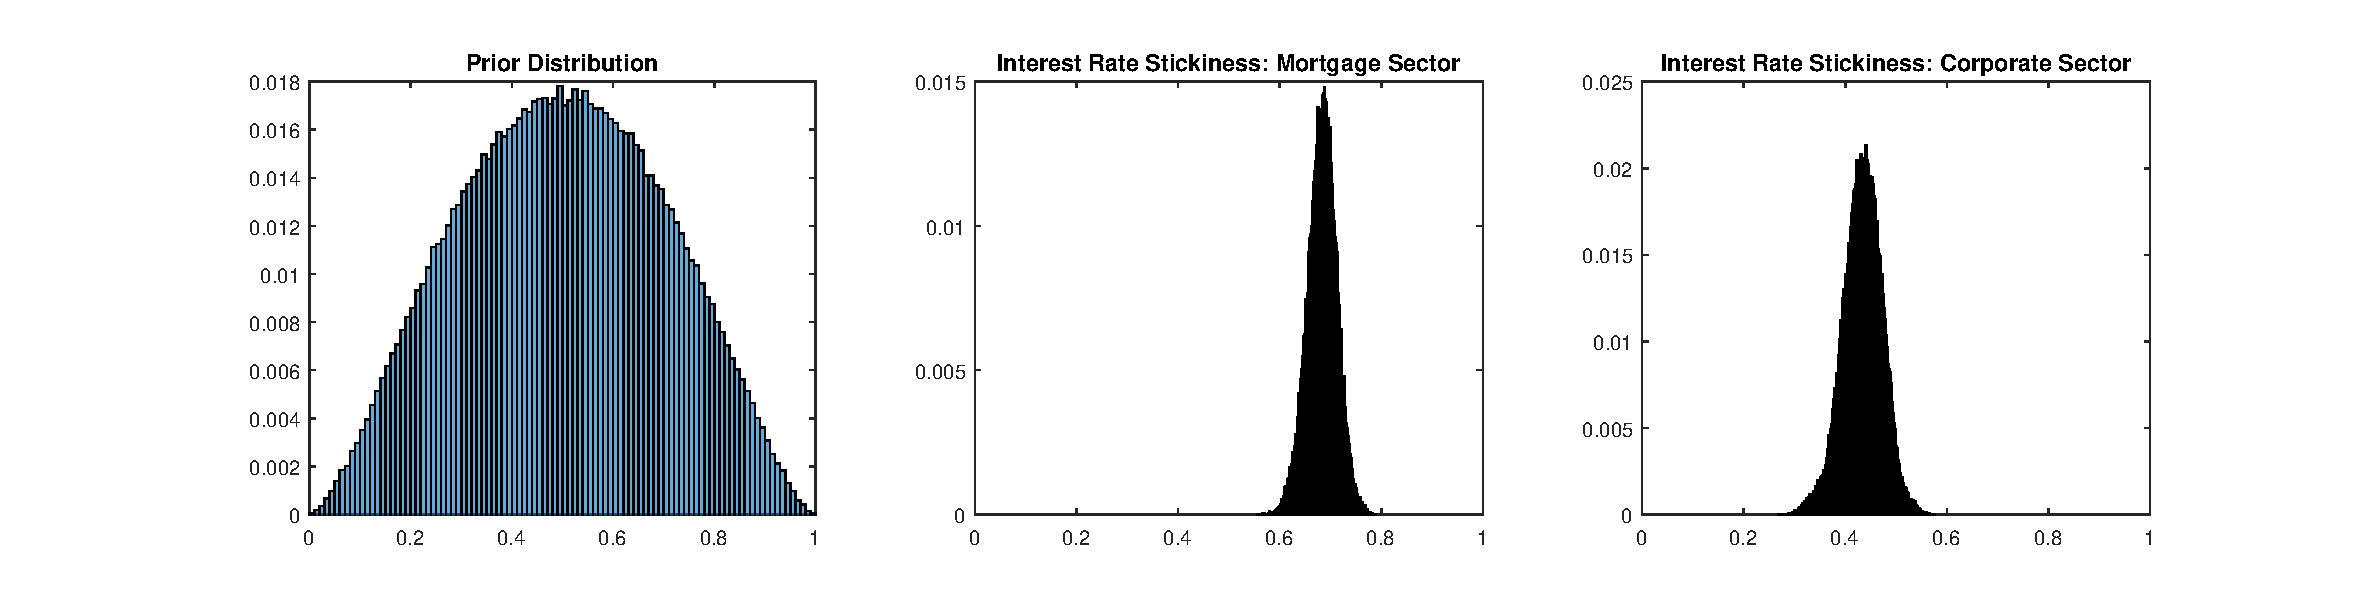
\includegraphics[scale=0.5]{posteriordistributions_calvo2.pdf}
\end{figure}


\section*{Estimated Shocks}

Figure ?? shows some of estimated shocks over estimated period, particularly those that play a dominant role over the Global Financial Crisis period. Accordingly, the drops in the macroeconomic variables come out as a combination of several adverse shocks in the model. On the housing side, there is an increase in the housing depreciation shock, which means there is suddenly an increase in the supply of houses available on the market\footnote{We estimated an alternative version of the model where the housing depreciation shock is replaced with a house price expectation shock, in which case a negative expectation shock replaces the role of the positive supply shock as depicted here.}. This is accompanied by a negative housing preference shock. This shift in the housing preference, ceteris paribus, would mean that households will shift their spending towards consumption rather than housing. Therefore the model generates a negative consumption preference shock to offset the impact of the housing preference shock on consumption. Together, these preference shocks can be interpreted as an increase in households' overall risk aversion that makes them less likely to purchase housing or spend on consumption as their income goes down. These shocks are accompanied by an increase in households' uncertainty (or risk) shock, which makes households more likely default other things being equal. Together, these shocks lead to an increase of around 5 \% in the default rate of households over the crisis period. A similar story emerges on the banking side, where we observe an increase in the bank uncertainty shock and a negative bank net worth shock. Together, these shocks lead to a gradual and moderate increase in the bank default rates from  0.1 \% to 0.2 \%. As such, the primary source of contraction in the model emerges as the adverse shocks on the household side that drive down the house prices and household income, leading to an increase in the household default rate and a reduction in the mortgage lending growth.

On the corporate side, we do not observe a discernible difference in business default rates. In order to match the observed drop in business lending rates, the model generates an increase in the capital depreciation shock. Because this creates a larger than observed impact on the real side of the economy in output, investment and consumption, there is a positive increase in the productivity shock to offset some of the impact of the capital depreciation shock. Th

\begin{figure}[H]
\label{smoothed_shocks_figure}
\caption{Smoothed Shocks}
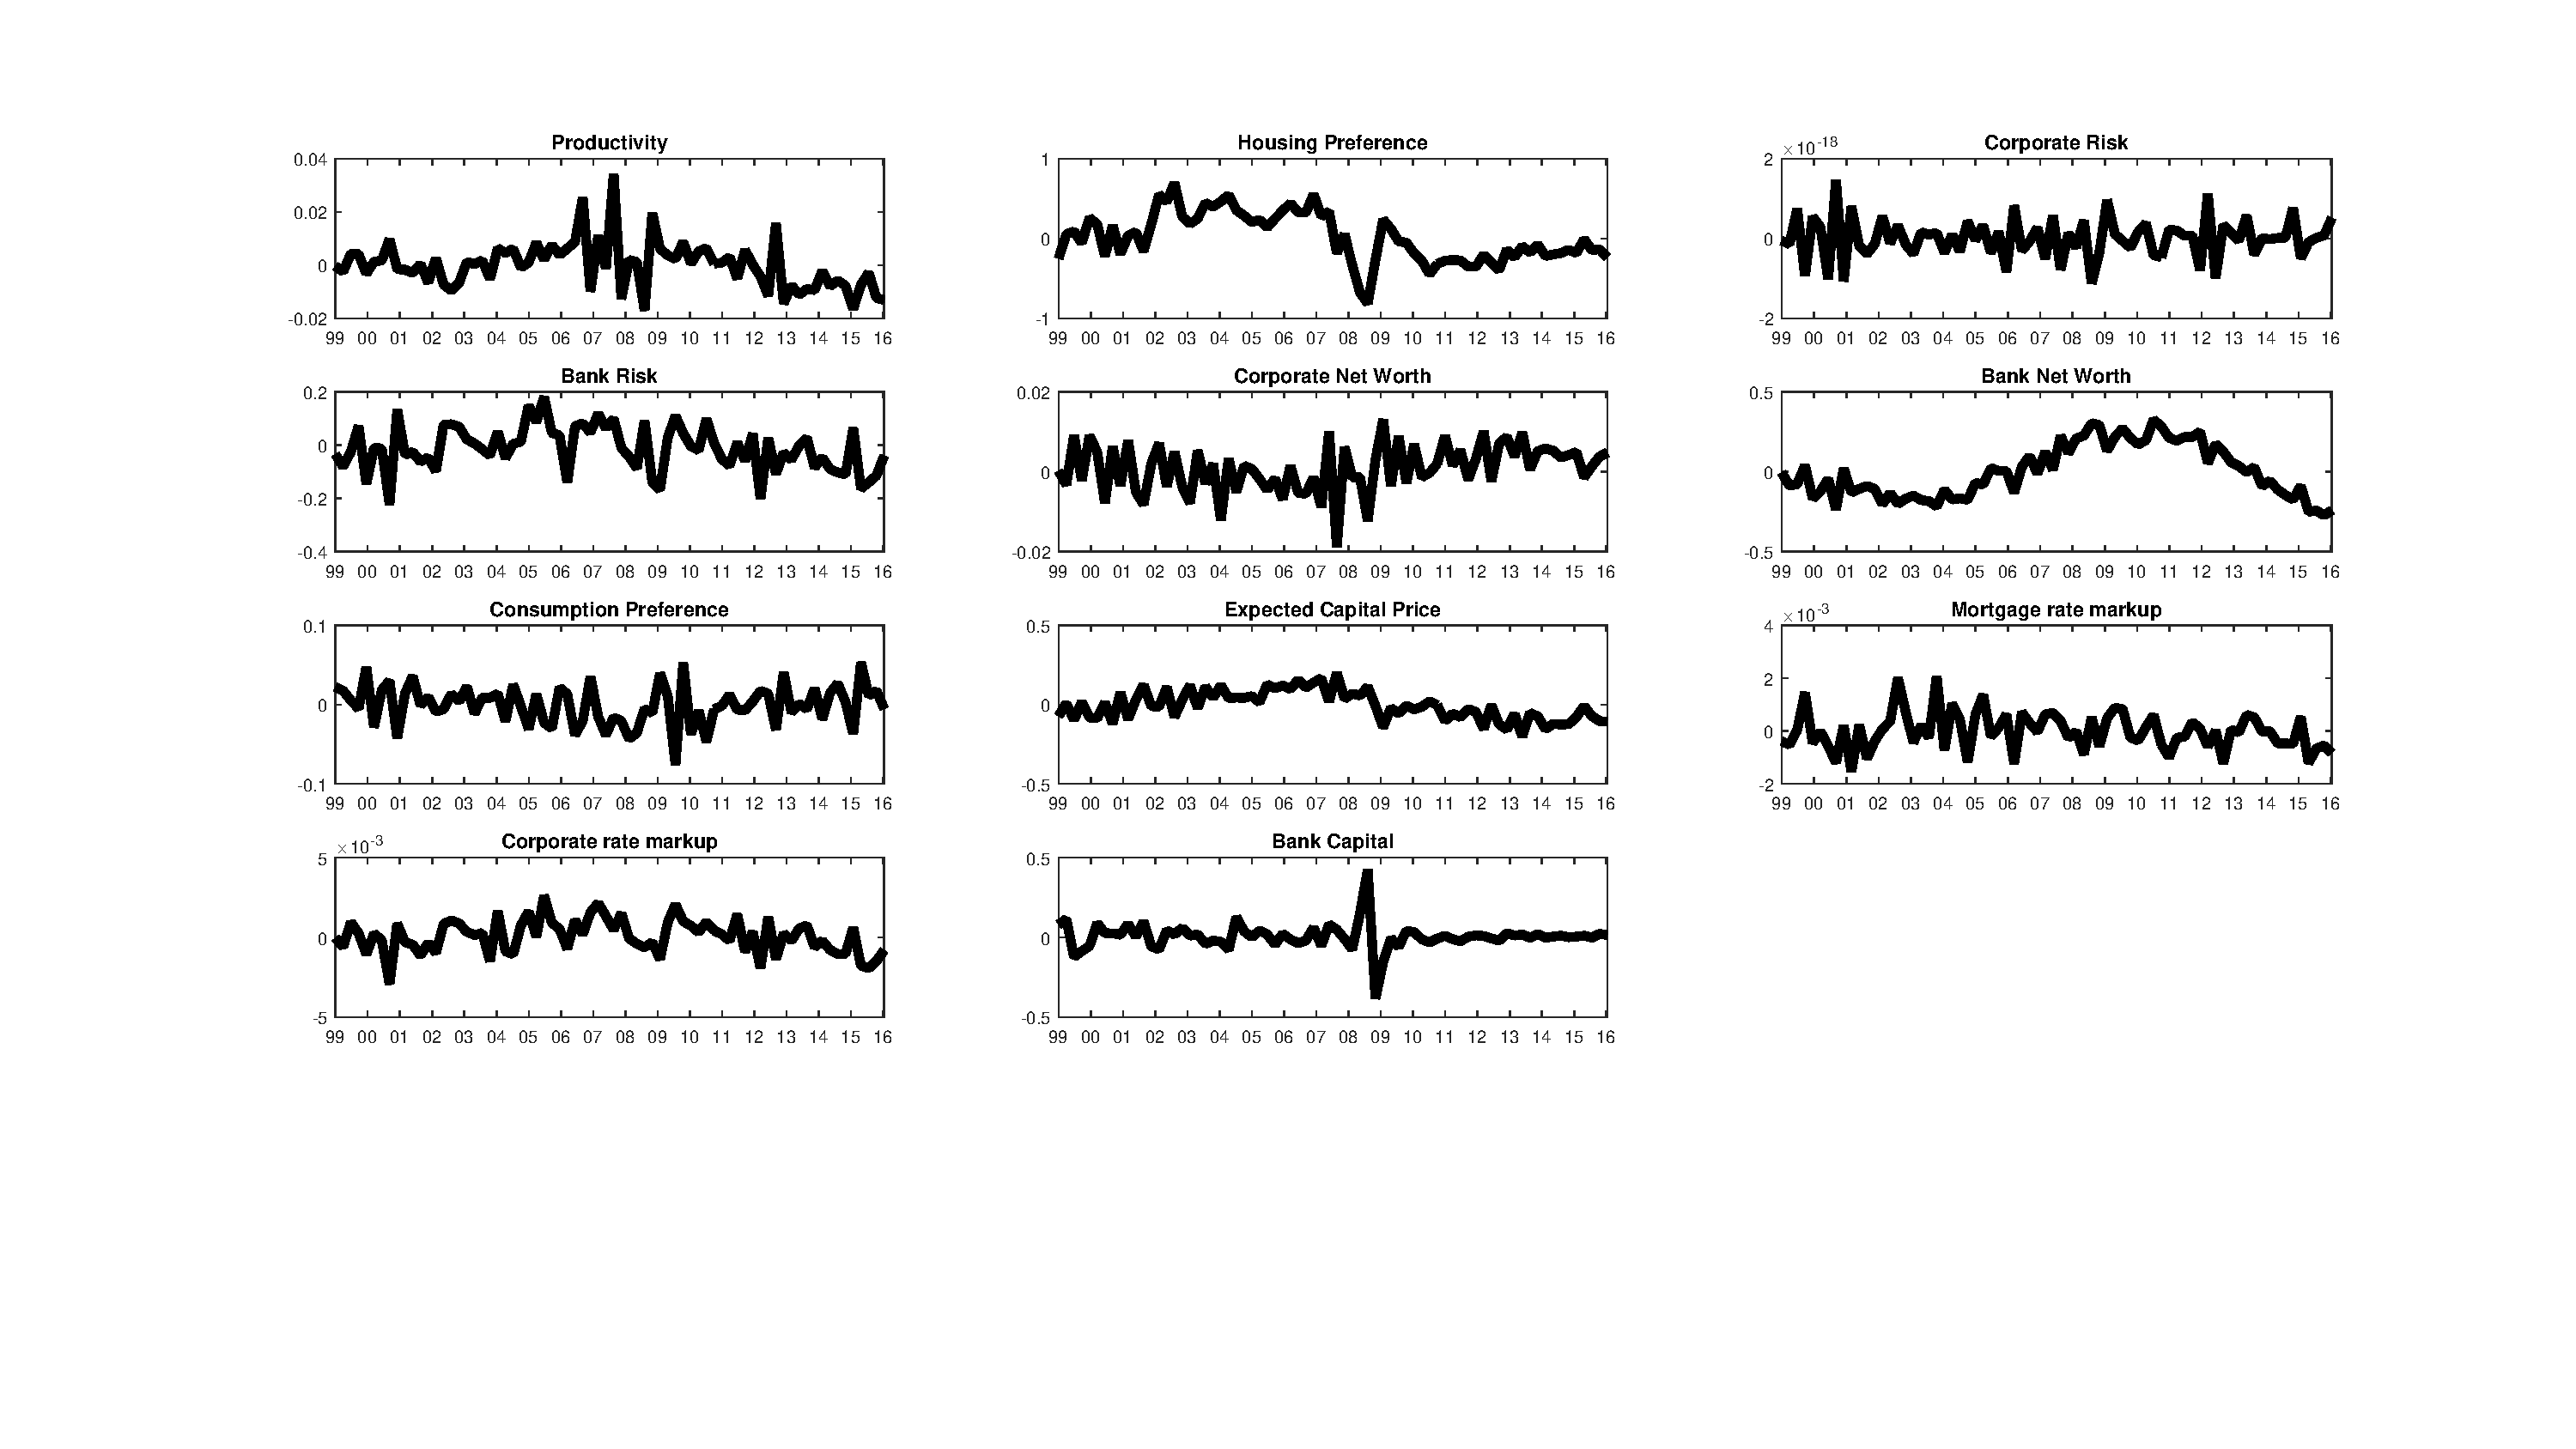
\includegraphics[scale=0.55]{smoothed_shocks.pdf}
\end{figure}



\section*{Variance Decompositions}

%depreciation shocks do two things: it increases the available stock of housing/capital, and directly reduces the rate of return on housing/corporate
%portfolio. Therefore for all intents and purposes, these resemble price expectations/stock market shocks?


%business lending rate and output growth only is probably sufficient for this part. 


To illustrate which shocks are important in driving the business cycle, Figures \ref{decomp_dbe_figure} and \ref{decomp_dy_figure} show the historical variance decompositions of business lending growth and output growth respectively. We select these two variables since they are representative of the financial and real sides of the economy respectively. The growth of business lending is mainly driven by depreciation and net worth shocks. Productivity, bank capital and uncertainty shocks also play a smaller role in driving the growth of business lending. The large drop in business lending over the crisis period emerges mainly as a reversal in the capital depreciation shock. 



  On the financial side, we focus on growth of business lending and house price growth, which are representative in terms of which shocks play a dominant role. 
 The growth rate of business lending is mainly driven by depreciation and productivity shocks, where the drop over the crisis period is driven mainly by the capital depreciation shock. The growth rate of housing, on the other hand, is driven primarily by the housing depreciation and preference shocks, where the drop over the crisis period emerges as a combination of these two shocks. The housing depreciation shock and the drop in house price growth feeds back positively into business lending rate, whereas the feedback from capital depreciation shock into house price growth (or the mortgage lending rate) is relatively small. There is also a small impact from bank capital shocks on house price growth. 

On the real side of the economy, we focus on output and consumption growth. Overall, output growth is driven main by productivity and capital depreciation shocks, as would be expected given the above decompositions. Further, net worth and uncertainty shocks, and to a smaller extent preference shocks also emerge as drivers of output growth. Consumption growth yields a similar picture, where the role of uncertainty shocks become smaller. This is instead replaced by more dominant role for the preference shocks. 



%\begin{figure}[H]
%\centering
%\caption{Official Bank Rate}
%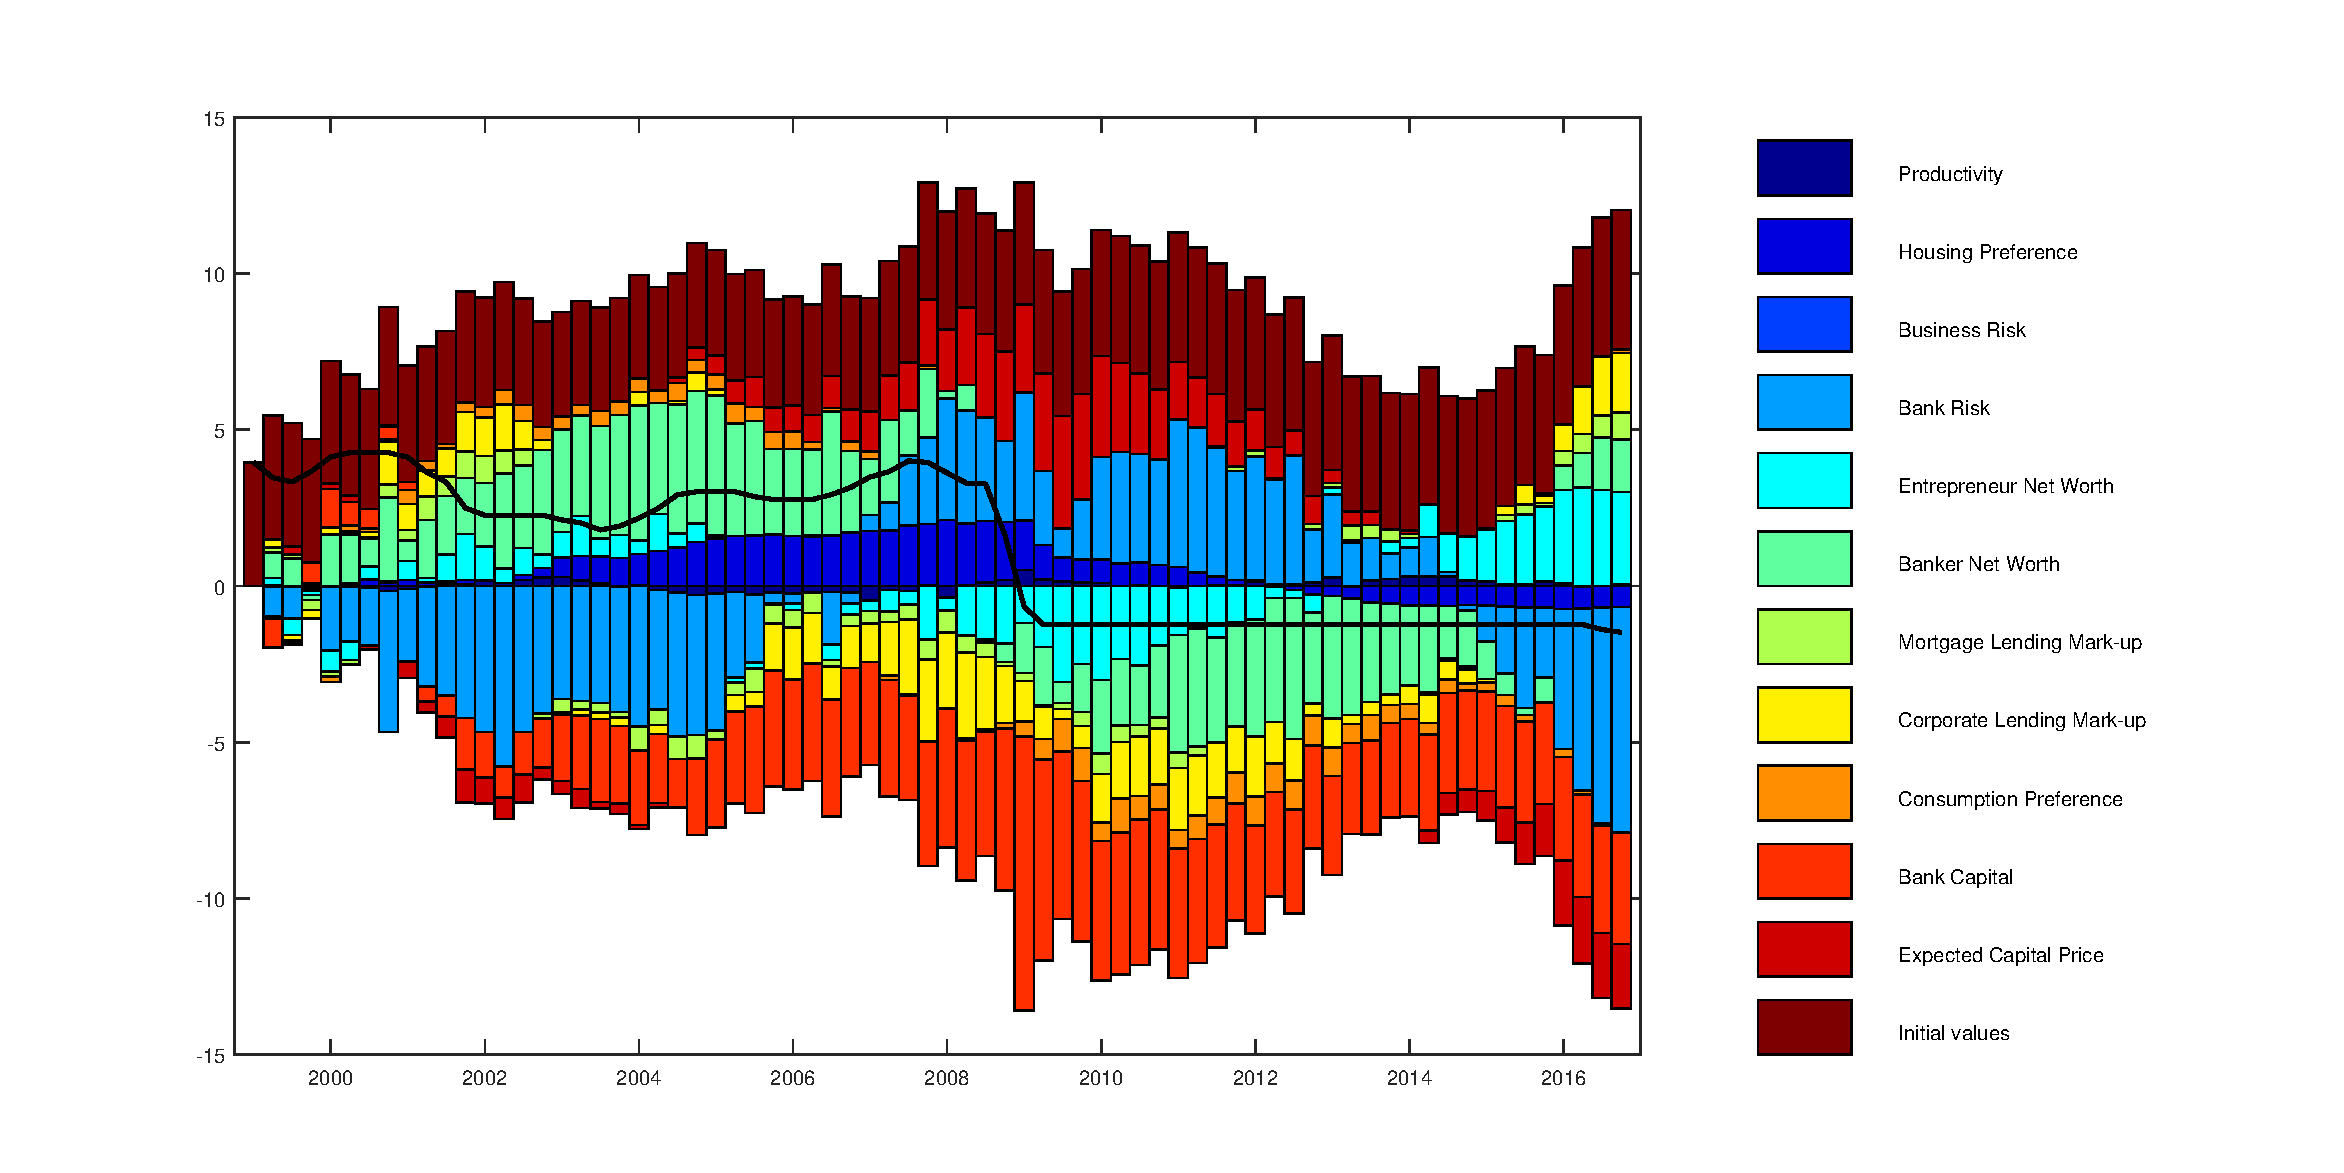
\includegraphics[scale=0.45]{decomp_bank_rate.pdf}
%\end{figure}


%\begin{figure}[H]
%\centering
%\caption{Mortgage Lending Rate}
%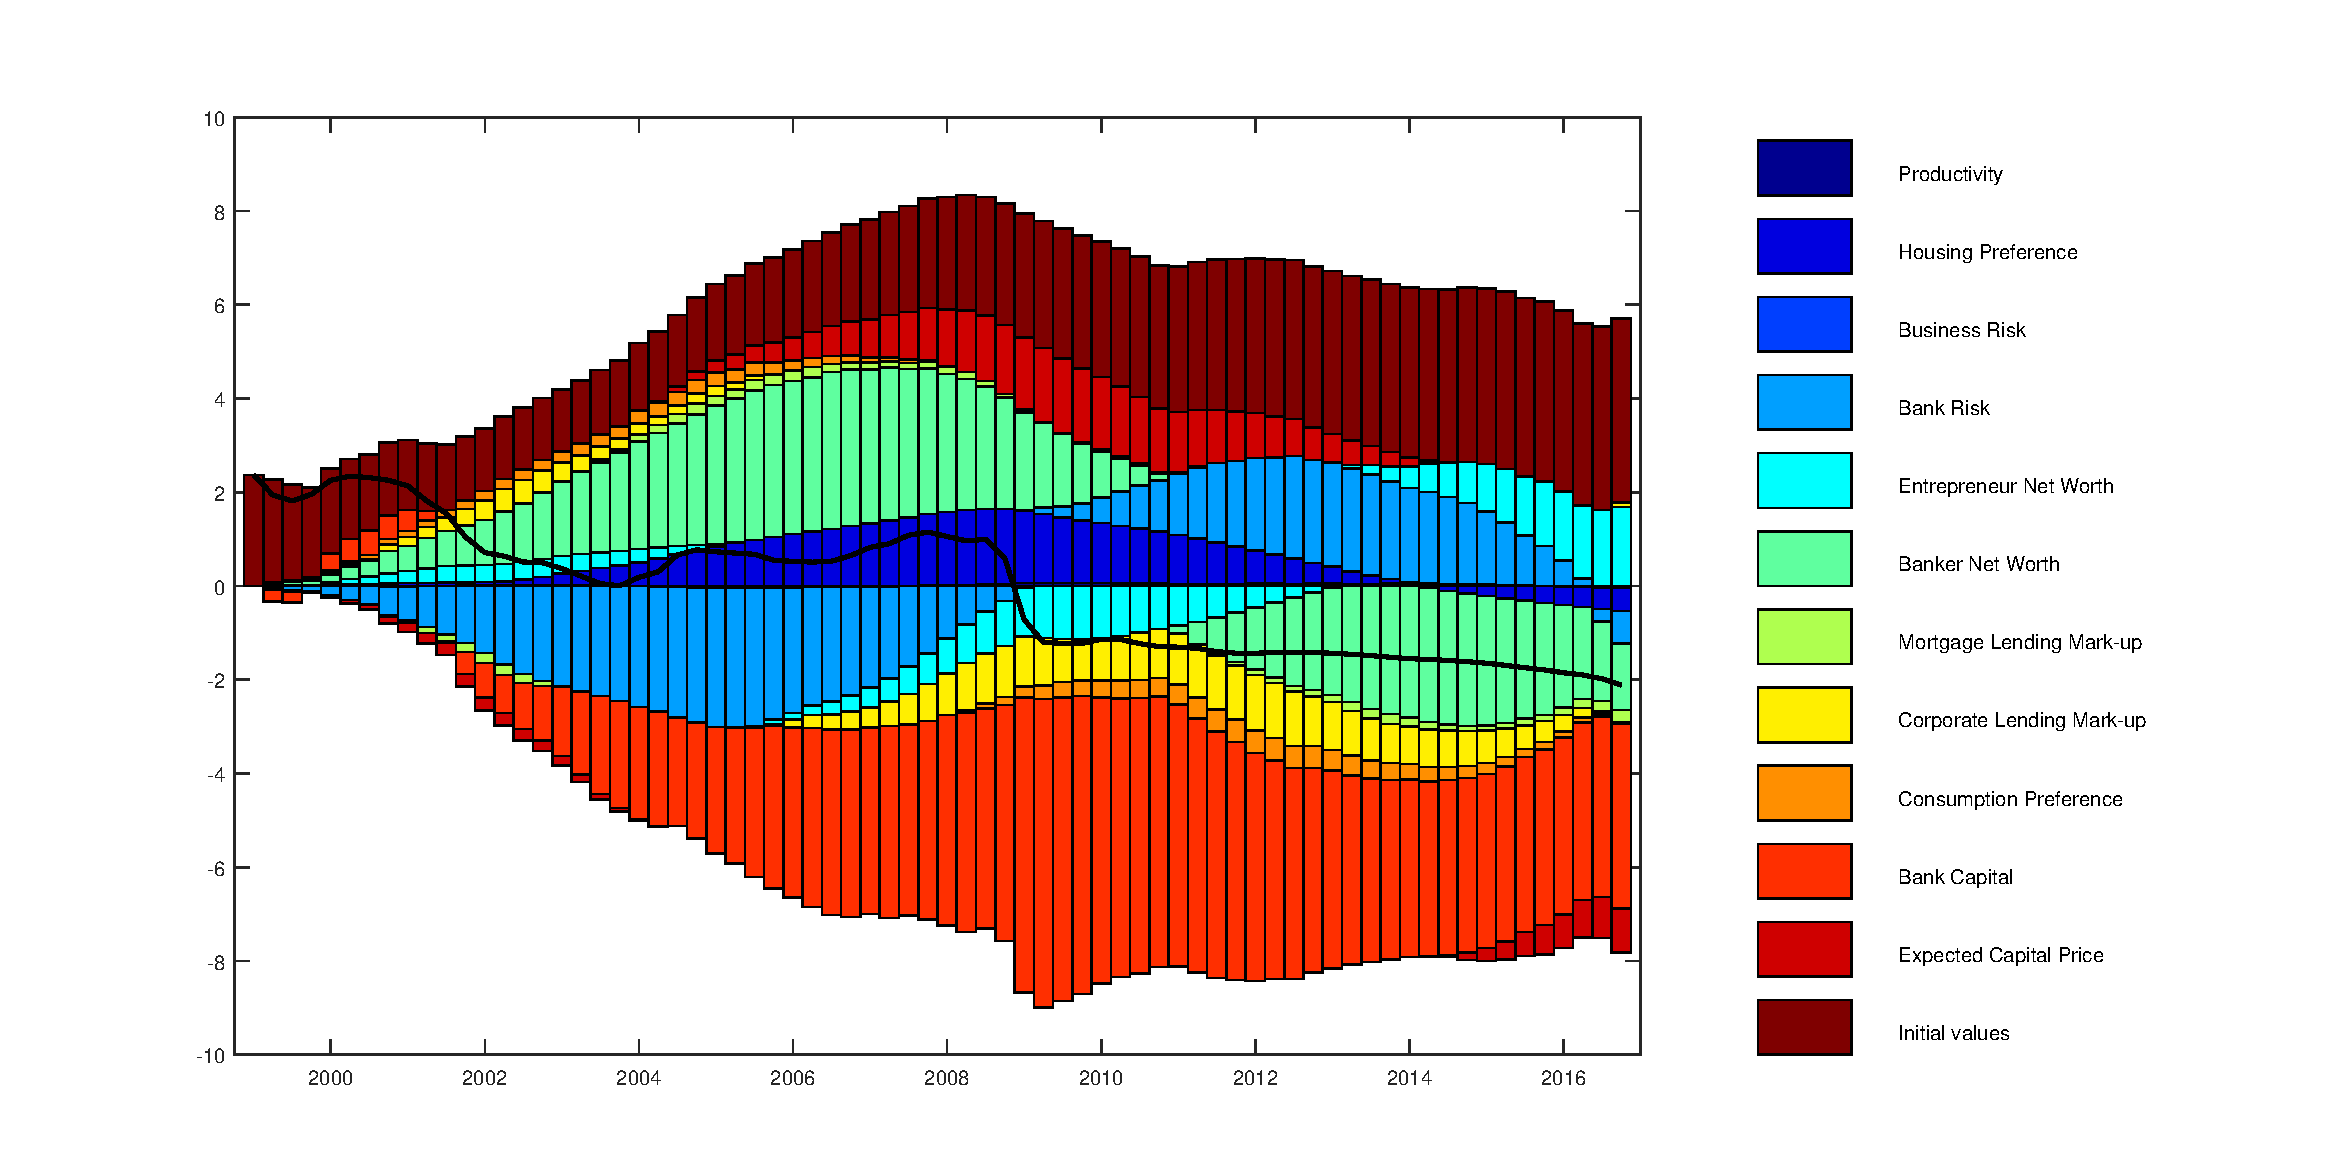
\includegraphics[scale=0.45]{decomp_int_rate_HH.pdf}
%\end{figure}

%\begin{figure}[H]
%\centering
%\caption{Corporate Lending Rate}
%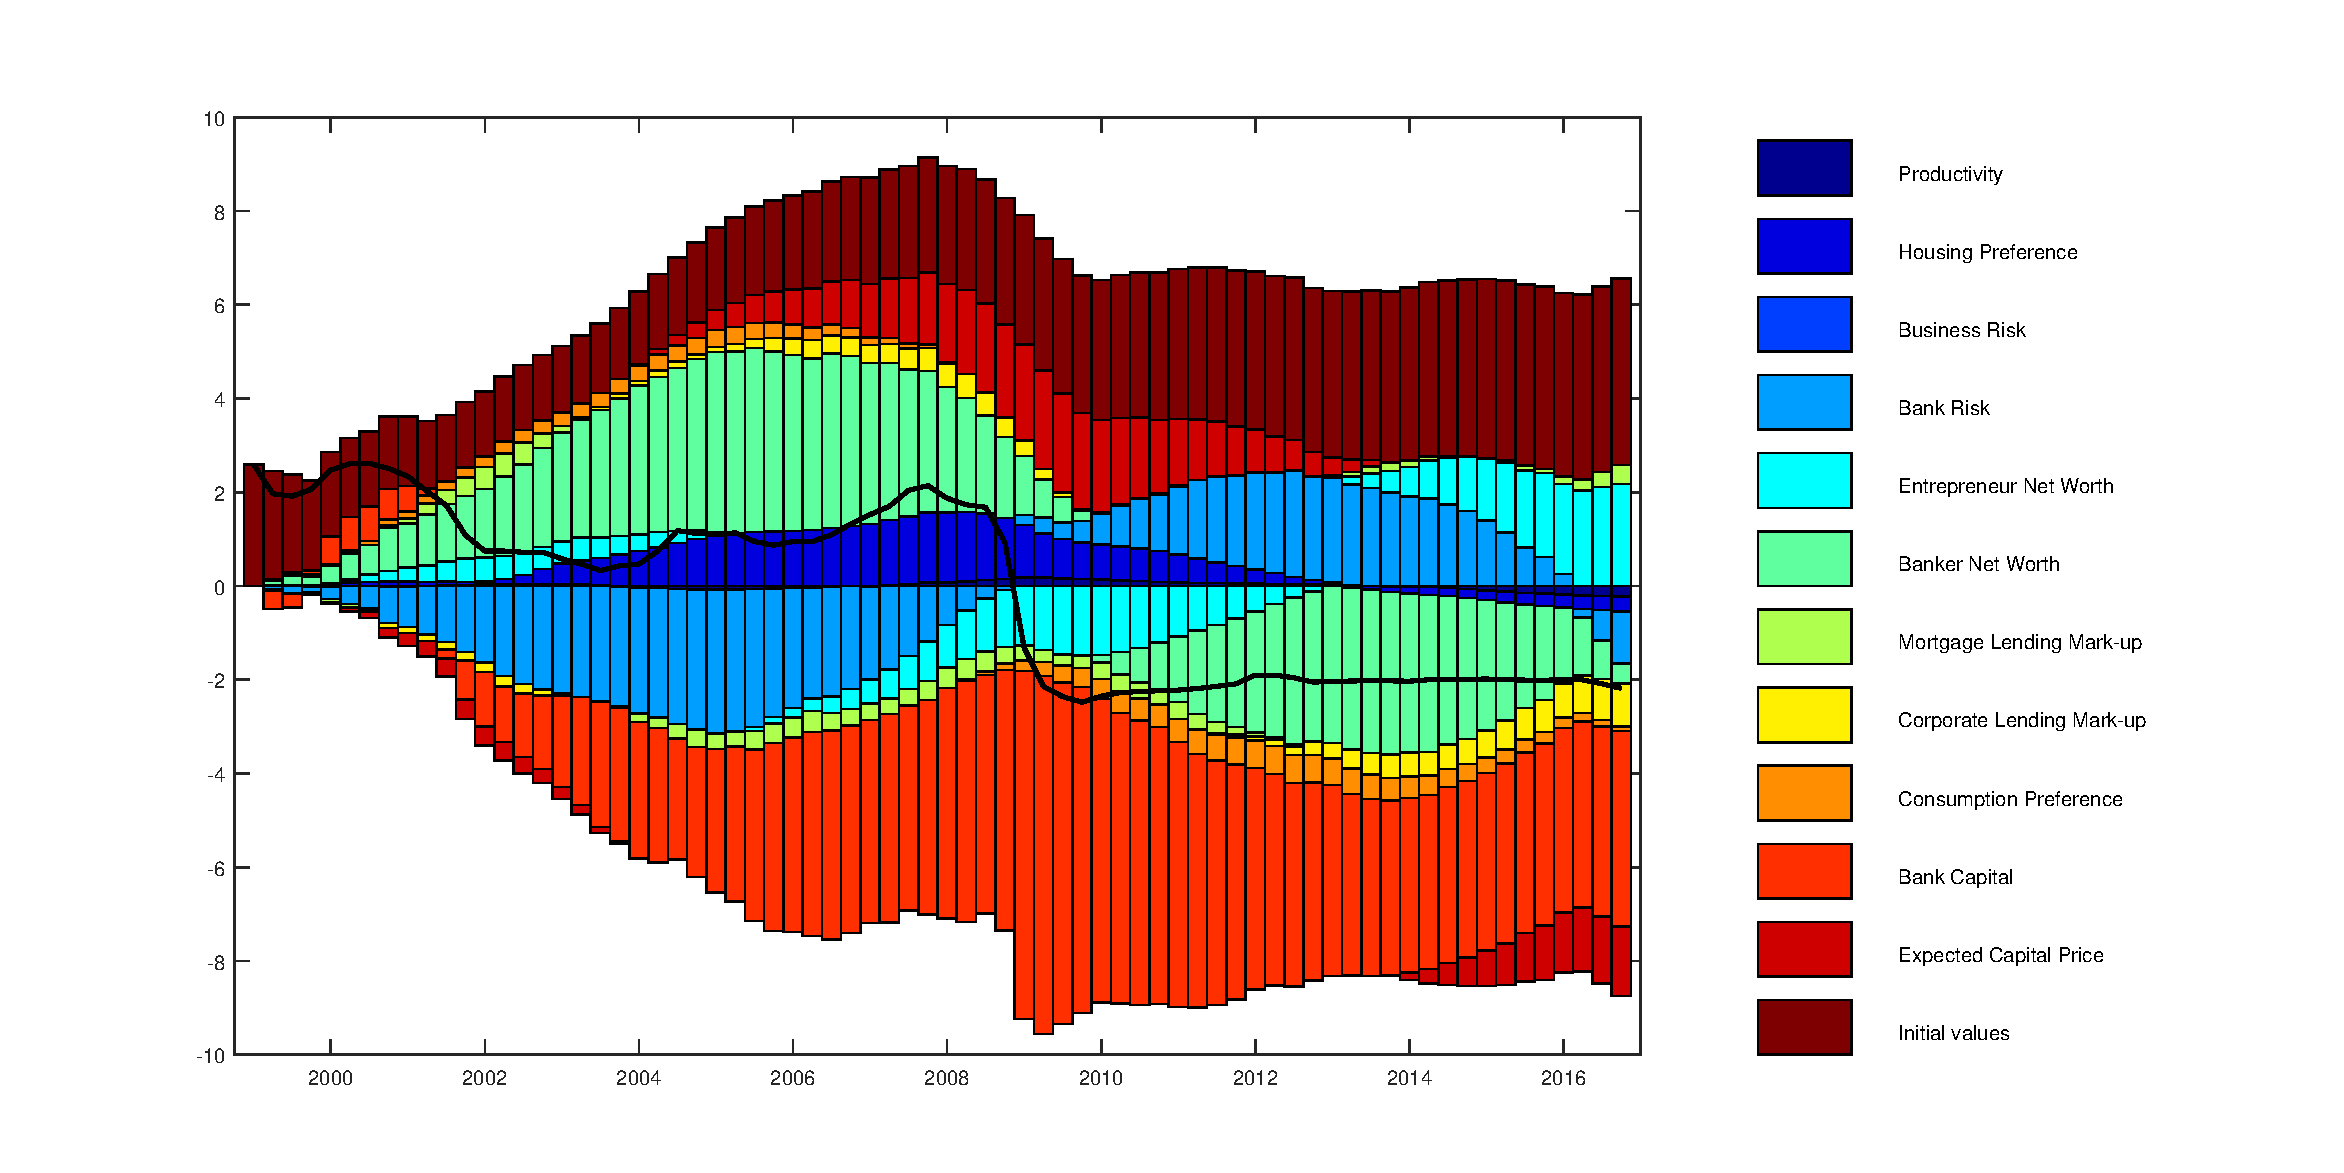
\includegraphics[scale=0.45]{decomp_int_rate_business.pdf}
%\end{figure}



\begin{figure}[H]
\centering
\caption{Growth of Business Lending}
\label{decomp_dbe_figure}
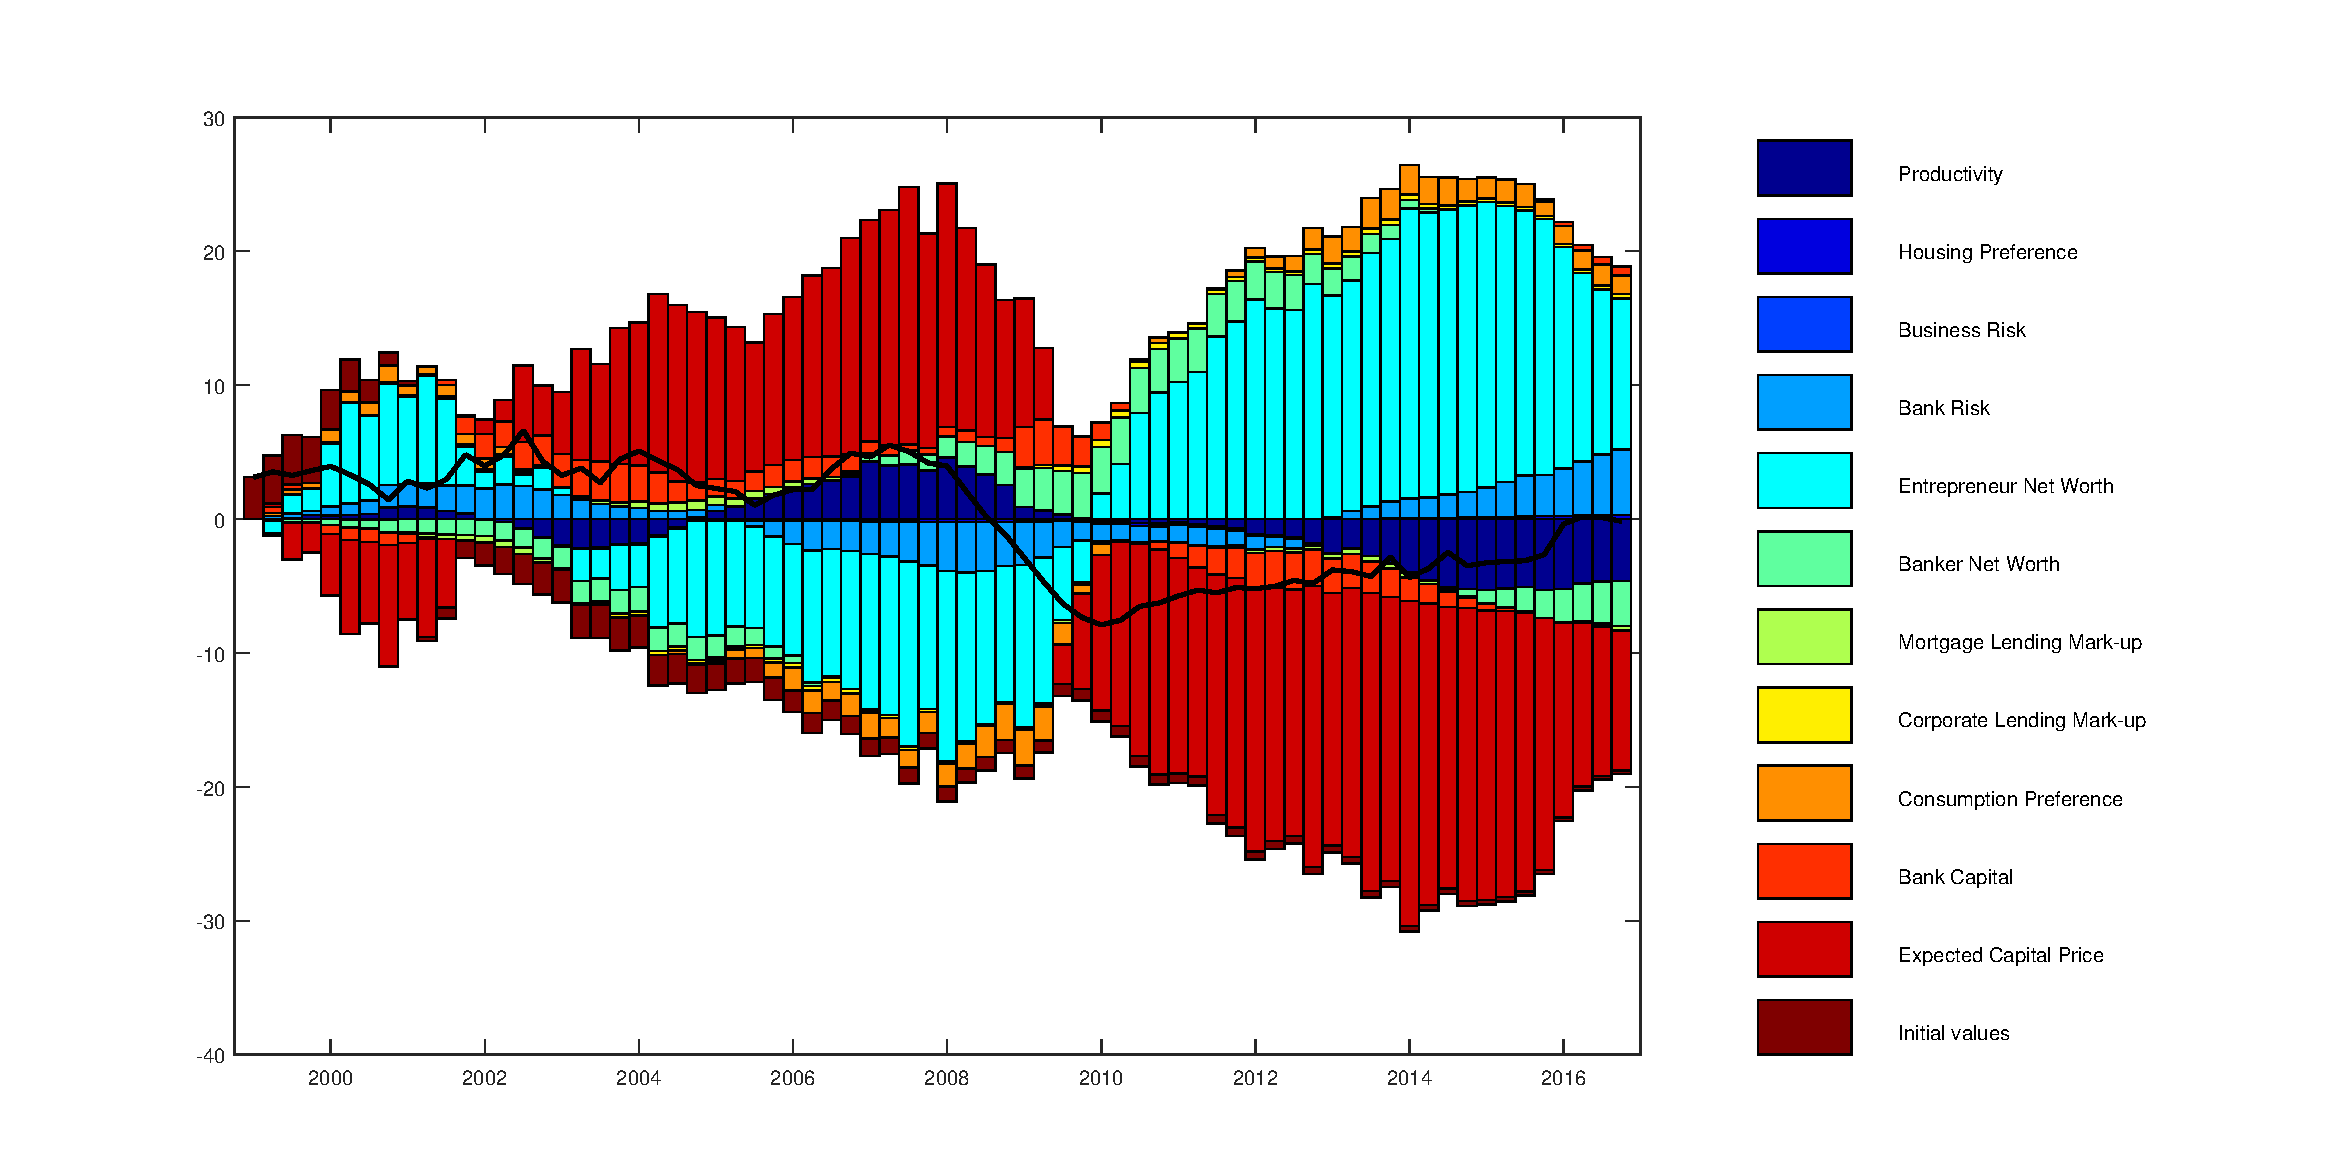
\includegraphics[scale=0.45]{decomp_dbe.pdf}
\end{figure}


%\begin{figure}[H]
%\centering
%\caption{Growth of Mortgage Lending}
%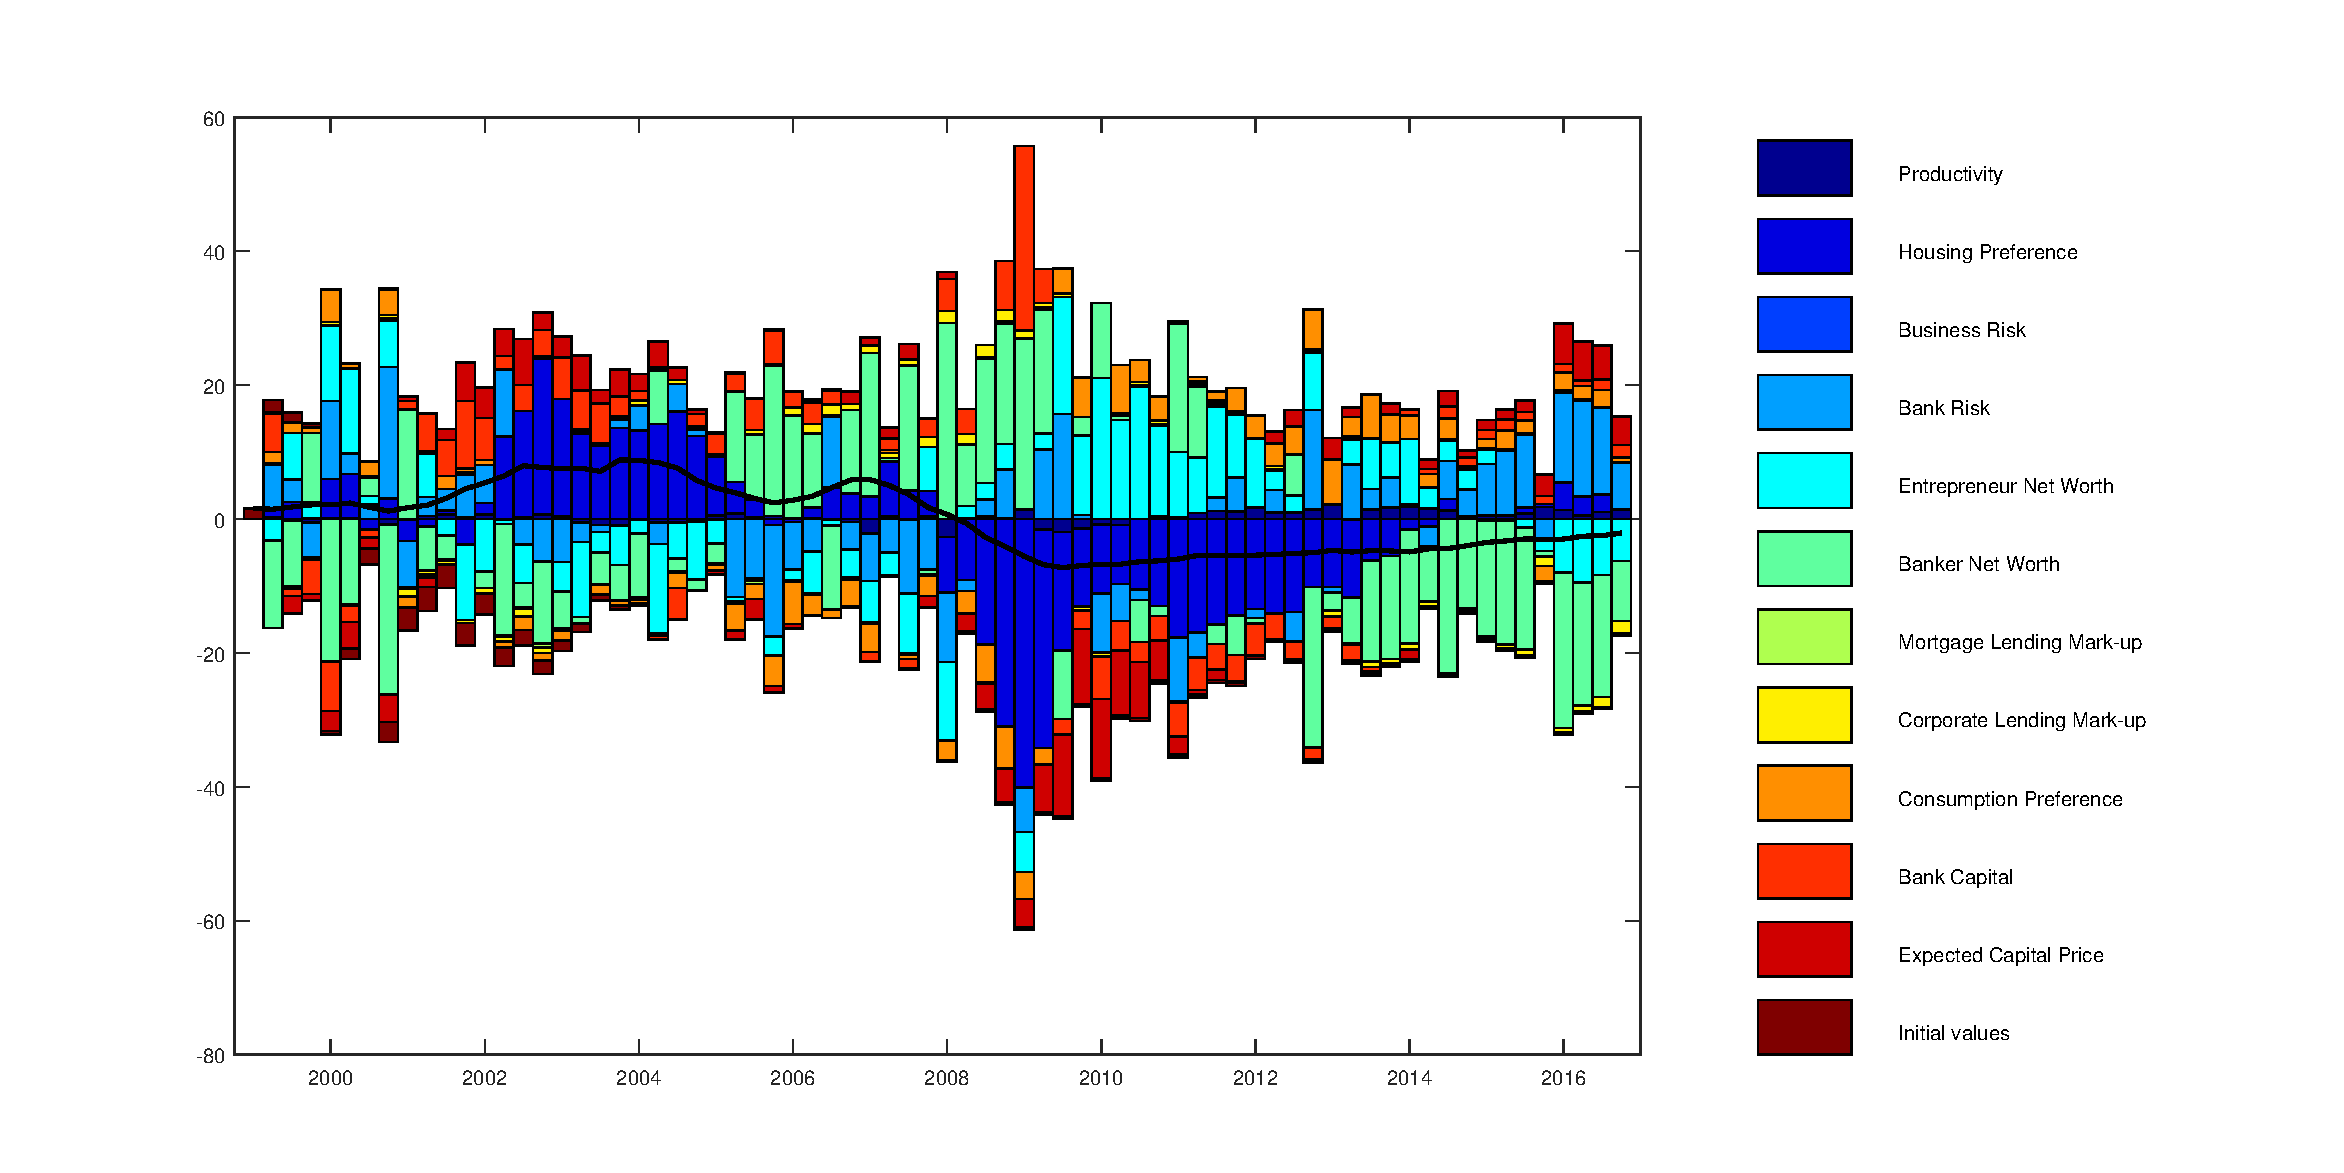
\includegraphics[scale=0.45]{decomp_dbm.pdf}
%\end{figure}


%\begin{figure}[H]
%\centering
%\caption{House Price Growth}
%\includegraphics[scale=0.45]{decomp_dqH.pdf}
%\end{figure}




%\begin{figure}[H]
%\centering
%\caption{Investment Growth}
%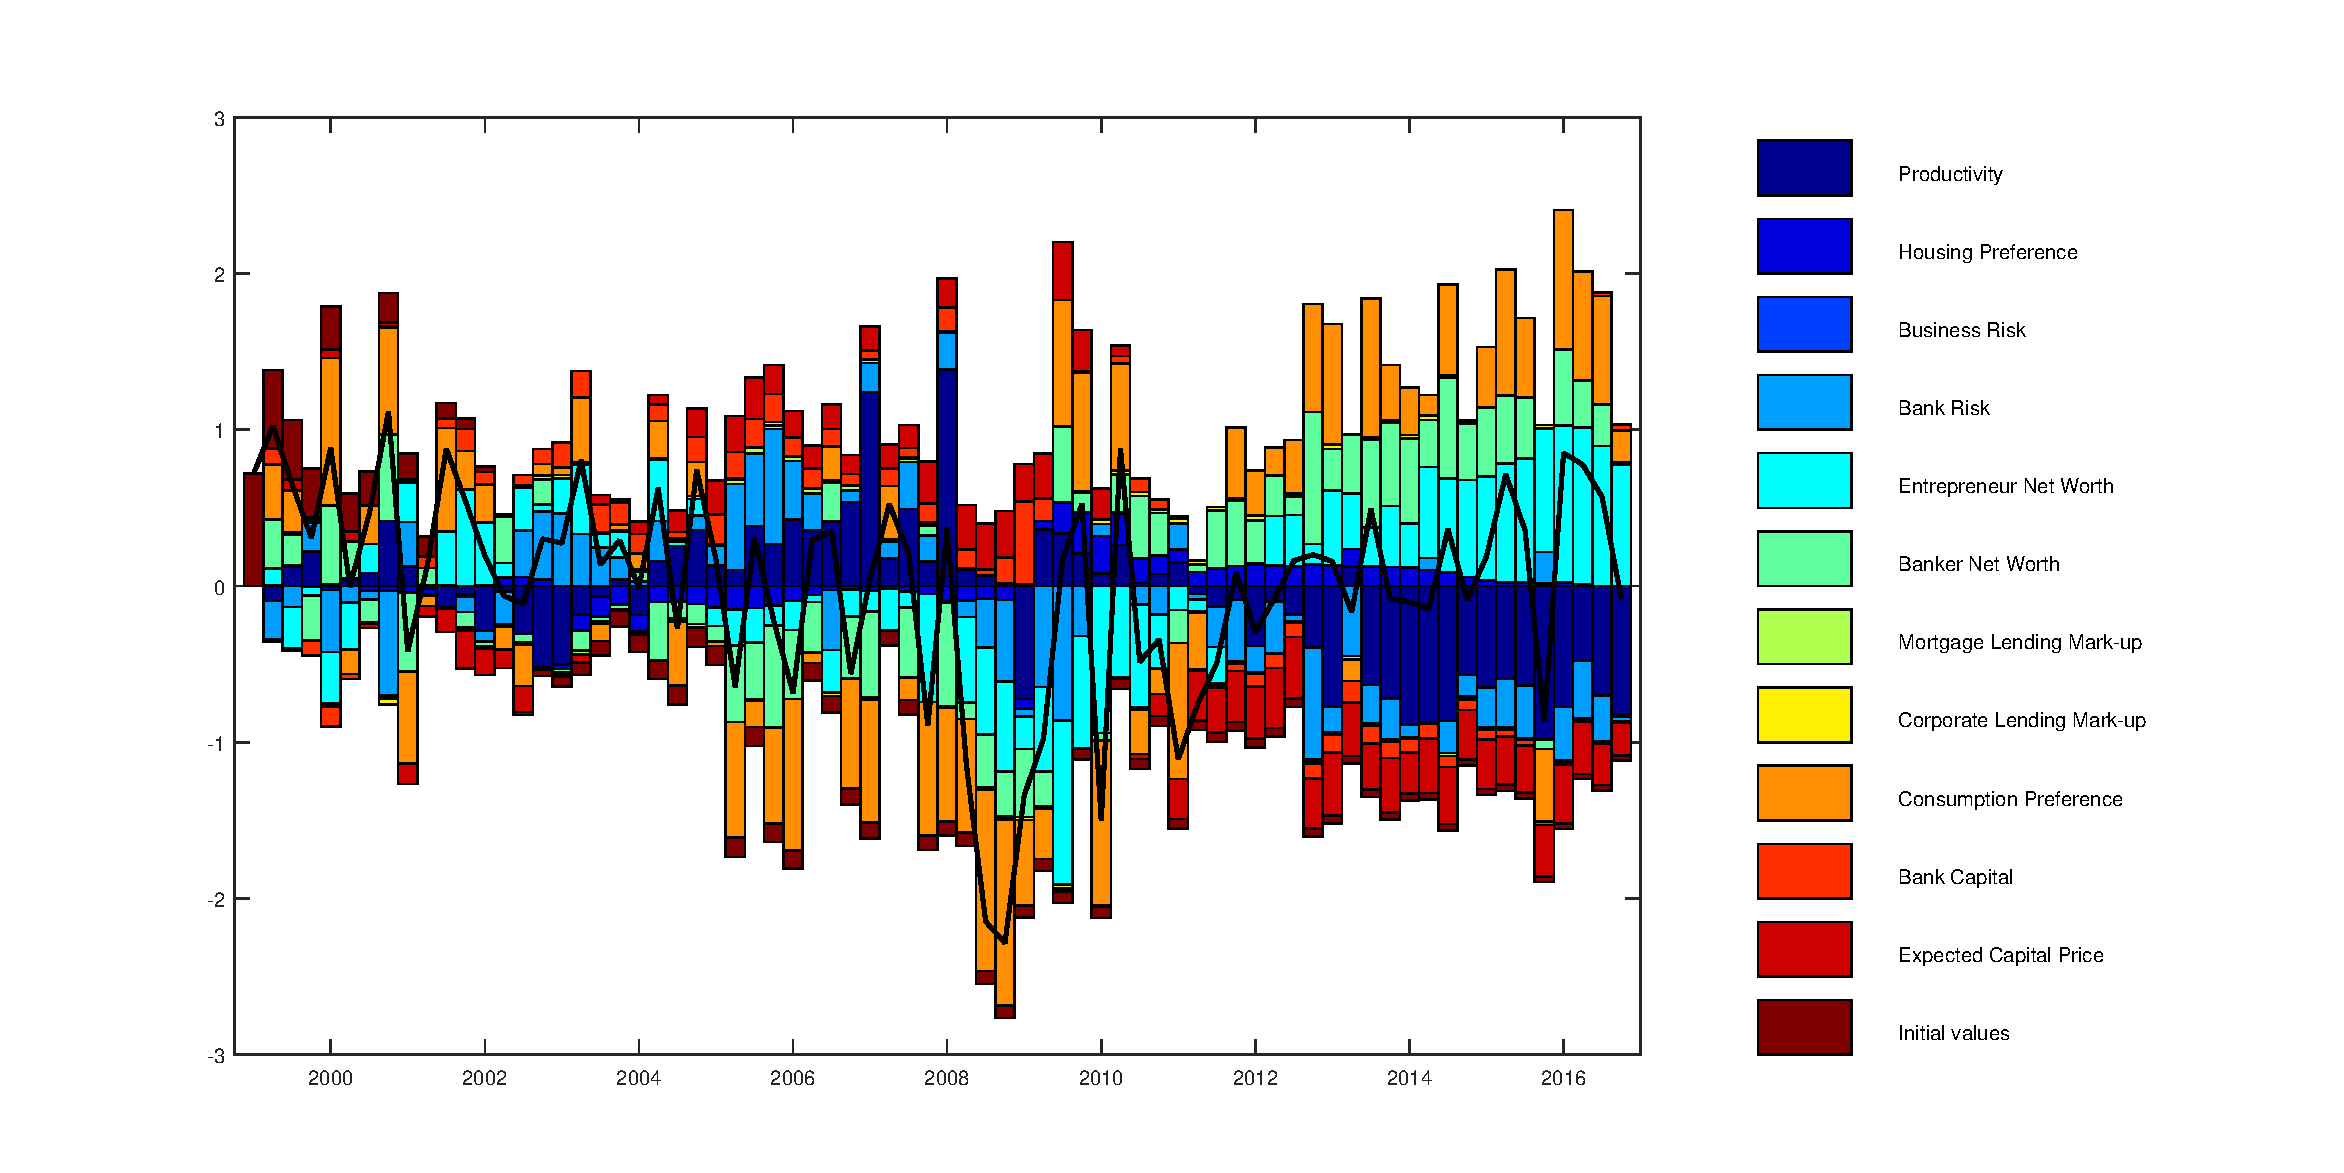
\includegraphics[scale=0.45]{decomp_dinve.pdf}
%\end{figure}



\begin{figure}[H]
\centering
\caption{Output Growth}
\label{decomp_dy_figure}
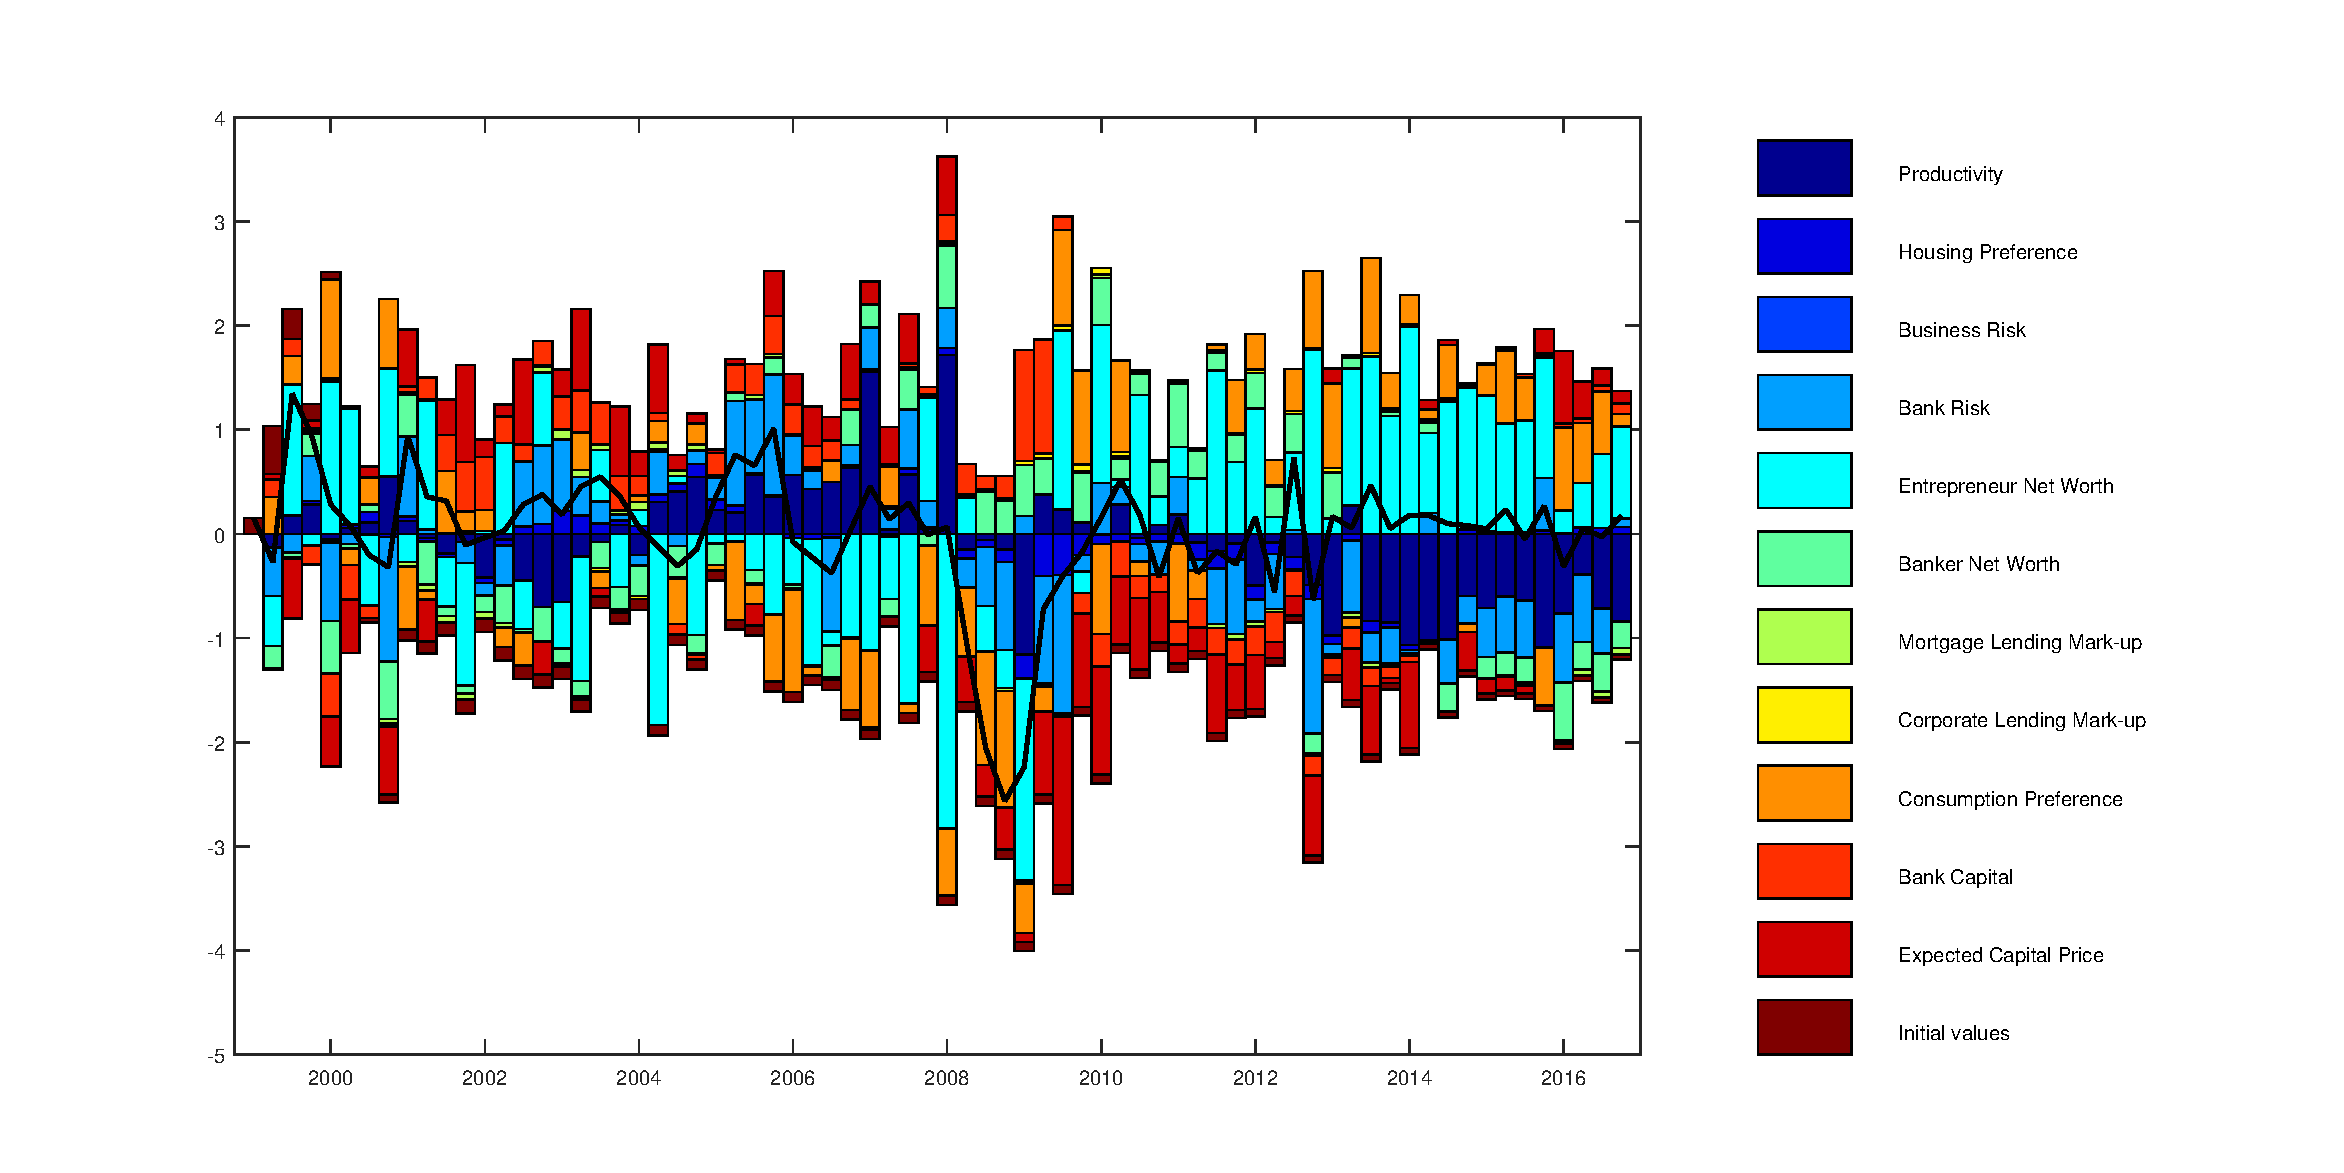
\includegraphics[scale=0.45]{decomp_dy.pdf}
\end{figure}

%\begin{figure}[H]
%\centering
%\caption{Consumption Growth}
%\label{decomp_dc_figure}
%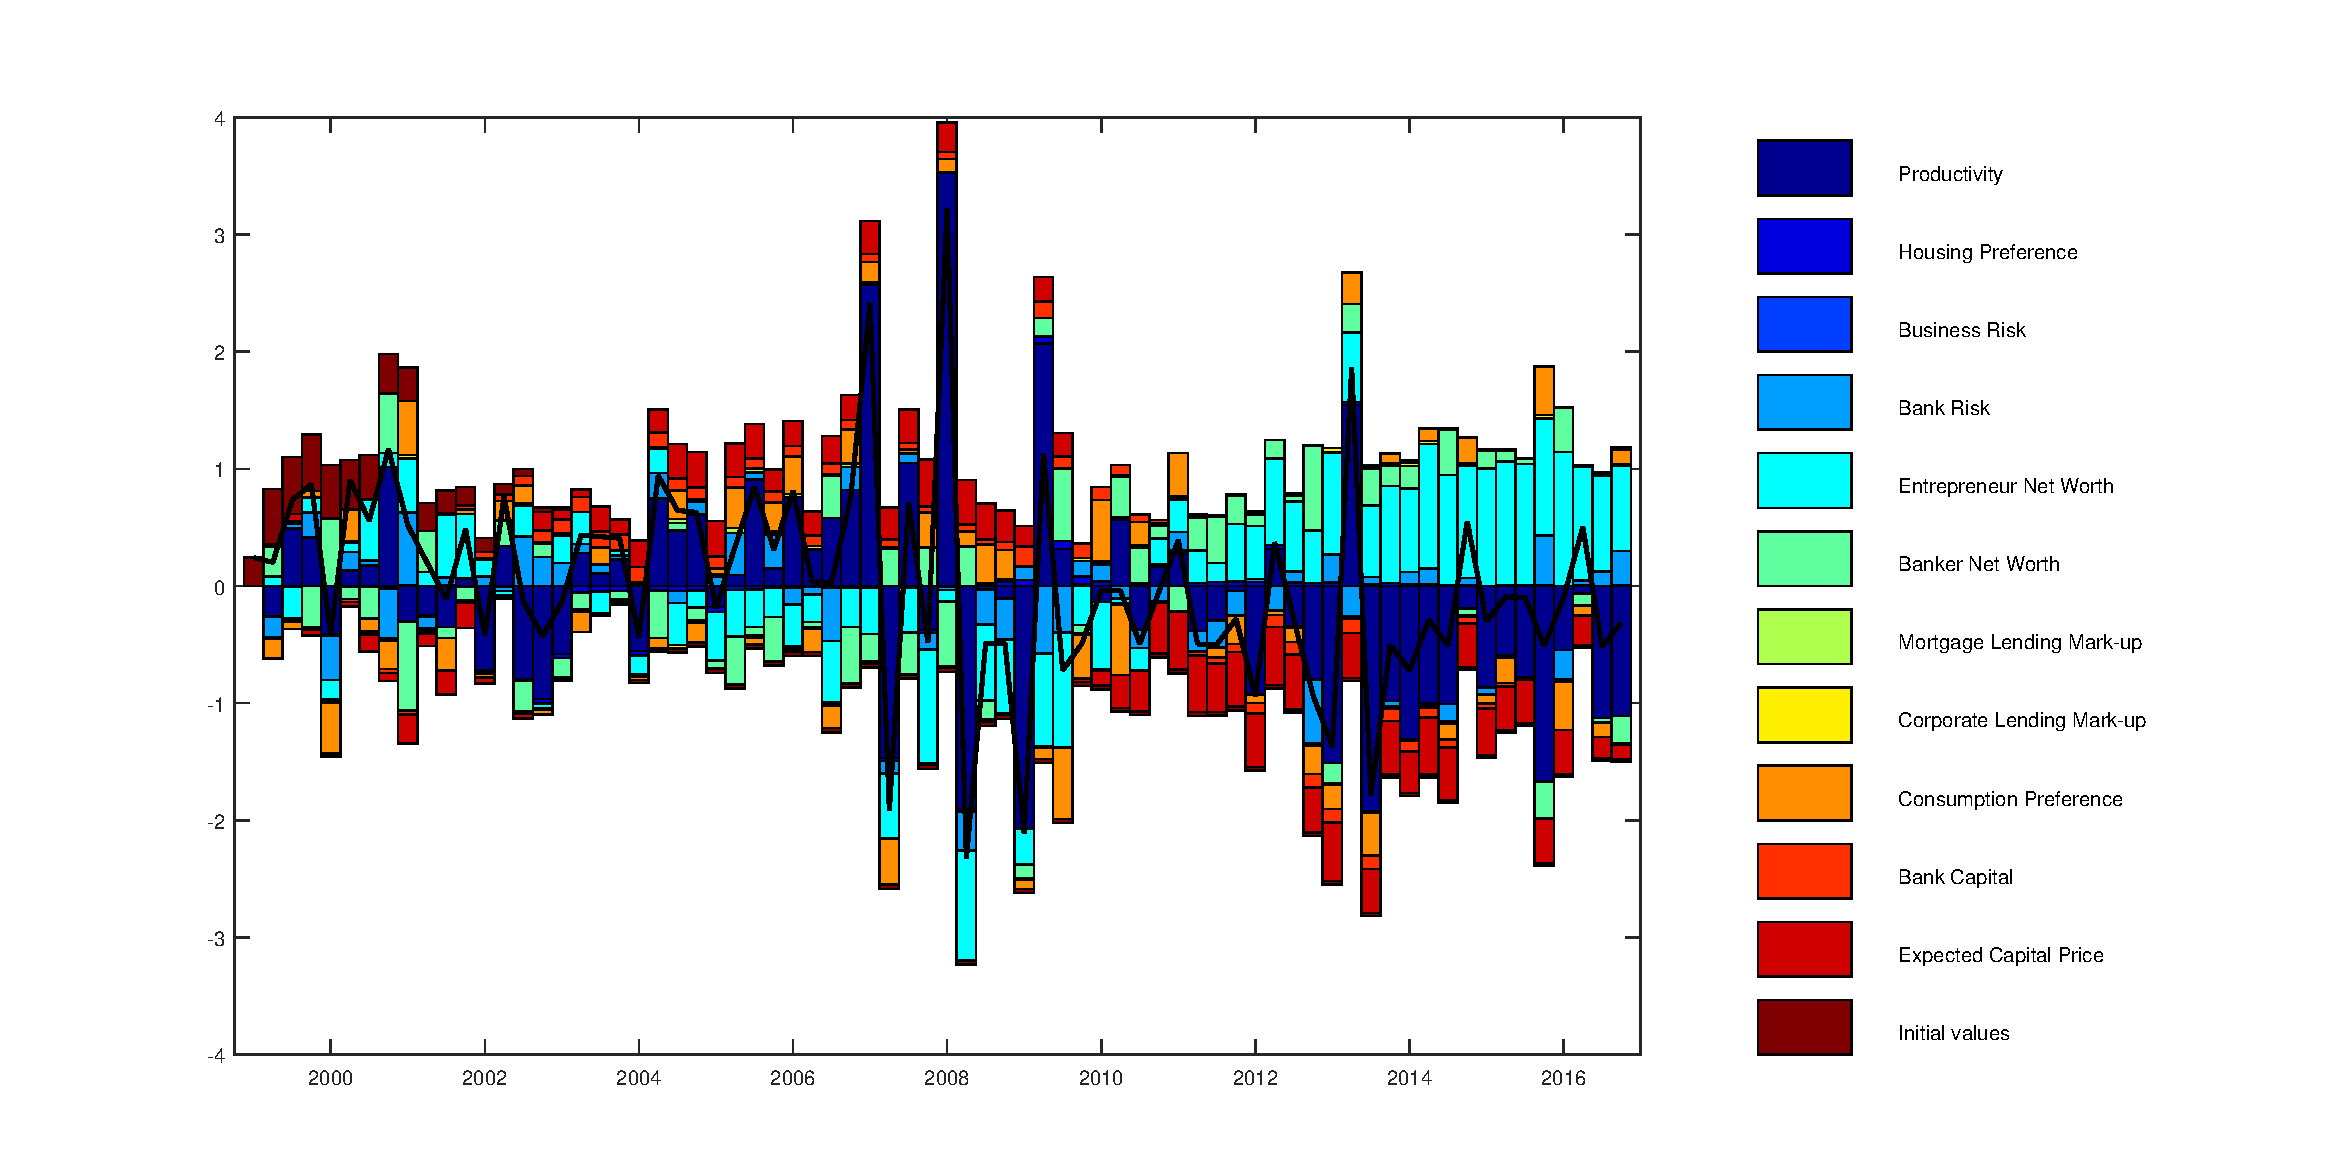
\includegraphics[scale=0.45]{decomp_dc.pdf}
%\end{figure}

%\begin{figure}[H]
%\centering
%\caption{Wage Growth}
%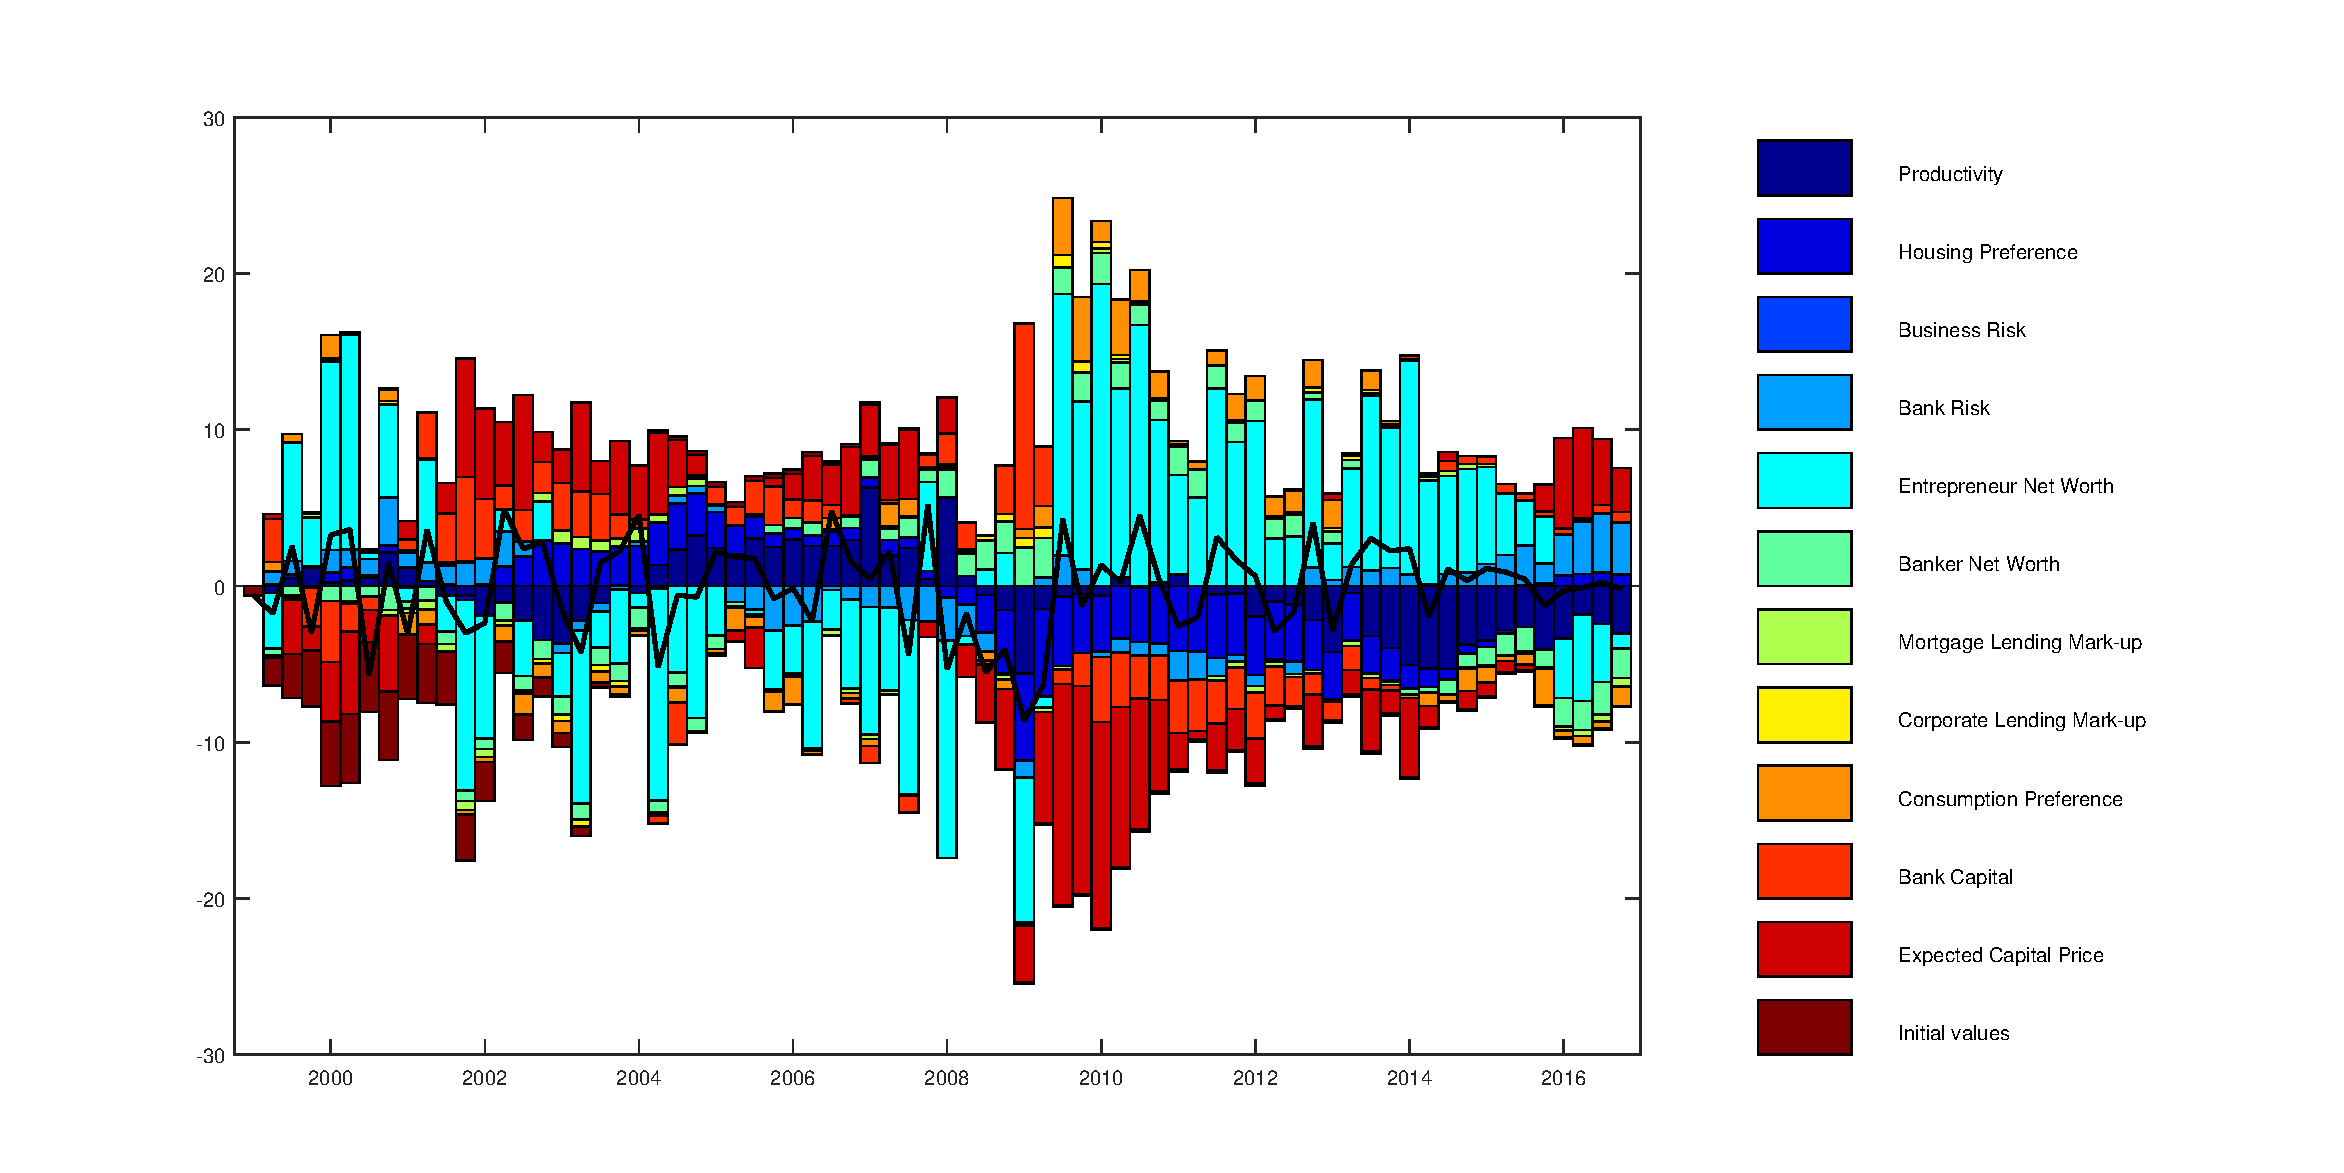
\includegraphics[scale=0.45]{decomp_dw.pdf}
%\end{figure}


\section*{Impulse Responses \& Interest Rate Stickiness}
%J-shock looks better than Hd here, because positive Hd--> boom in output not nice

Before analyzing macroprudential tools, we first investigate the impact of staggered interest rates on shock propagation. Figures ?? through ?? report the impulse responses of several variables to three shocks originating in different sectors of the economy: a negative housing preference shock in the mortgage sector and a capital depreciation shock in the corporate sector, both of which play important roles in driving the business cycle as we saw previously; and a negative bank capital shock in the banking sector which may be interpreted as a proxy for monetary policy shocks [DOES THE LAST SENTENCE MAKE SENSE?]. 

preference shock: households have a weaker preference for purchasing housing (or more adverse to purchasing housing) everything else equal. Therefore household borrowing decreases. Due to decreased housing demand, house prices go down. Interest rate stickiness has little effect on these two. The bank's response to decreased demand is to cut the interest rates, and the magnitude of this depends crucially on the degree of stickiness: the smallest change is clearly in the case where the Calvo probabilities are largest. The response of business borrowing also crucially depends on the stickiness: with small stickiness, the bank is able to shift its bundle towards corporate lending by cutting the interest rates, in which case there is a very little overall impact on business lending. When interest rates are sticky, the bank cannot adjust its rate as much as it would like, and as a result corporate lending goes down. As a result of this amplified impact on business lending, aggregate output  experiences larger drops as interest rate stickiness increases.
-->shock originating in the household sector, the biggest difference in IRFs in business borrowing since it takes longer to transmit through interest rates due to Calvo setting. 
(??? why is business borrowing going down in this case ???)


capital depreciation shock: business borrowing goes down since the return on equity on corporate investment is now smaller. Similar to above, the bank responds by cutting the interest rates, which crucially depends on the the degree of stickiness to boost demand. The response of mortgage rates depends on the degree of stickiness, but the overall impact is a reduction either initially or in the medium run (and the cumulative impact is a reduction in all cases). 
The largest impact on aggregate consumption and house prices is observed when interest rate stickiness is shut off in both sectors as one might expect. The spillover on aggregate output is rather small though, and it is similar in all cases. 
--> shock originating in the corporate sector, the biggest difference in IRFs in household borrowing and house prices since the transmission from one sector to the other affected by interest rates. The real effects (on output and consumption) are much smaller in this case compared to the housing preference shock. This might be due to the corporate interest rates already being small in the baseline case, so shutting it off does not have as large an effect.
--> shock originating in the corporate sector, the biggest difference in IRFs in household borrowing and house prices, since it takes longer for the shock to transmit to the other sector, same as the above argument.

negative bank capital shock: the bank would like to reduce its lending since it has less capital now, so its response is to increase the lending rates. When interest rates are stickier, it is not able to increase its interest rates as much. Therefore the impact on household and corporate borrowing, and therefore on aggregate output, is smaller with stickier interest rates. 
--> shock originating in the banking sector, both housing and corporate related IRFs reflect this since the shock now needs to transmit into both sectors through interest rates. Therefore we get the larger differences across the board in IRFs as opposed to the previous two shocks. 



\begin{figure}[H]
\centering
\caption{Negative Housing Preference Shock}
\label{stickinessJ_figure}
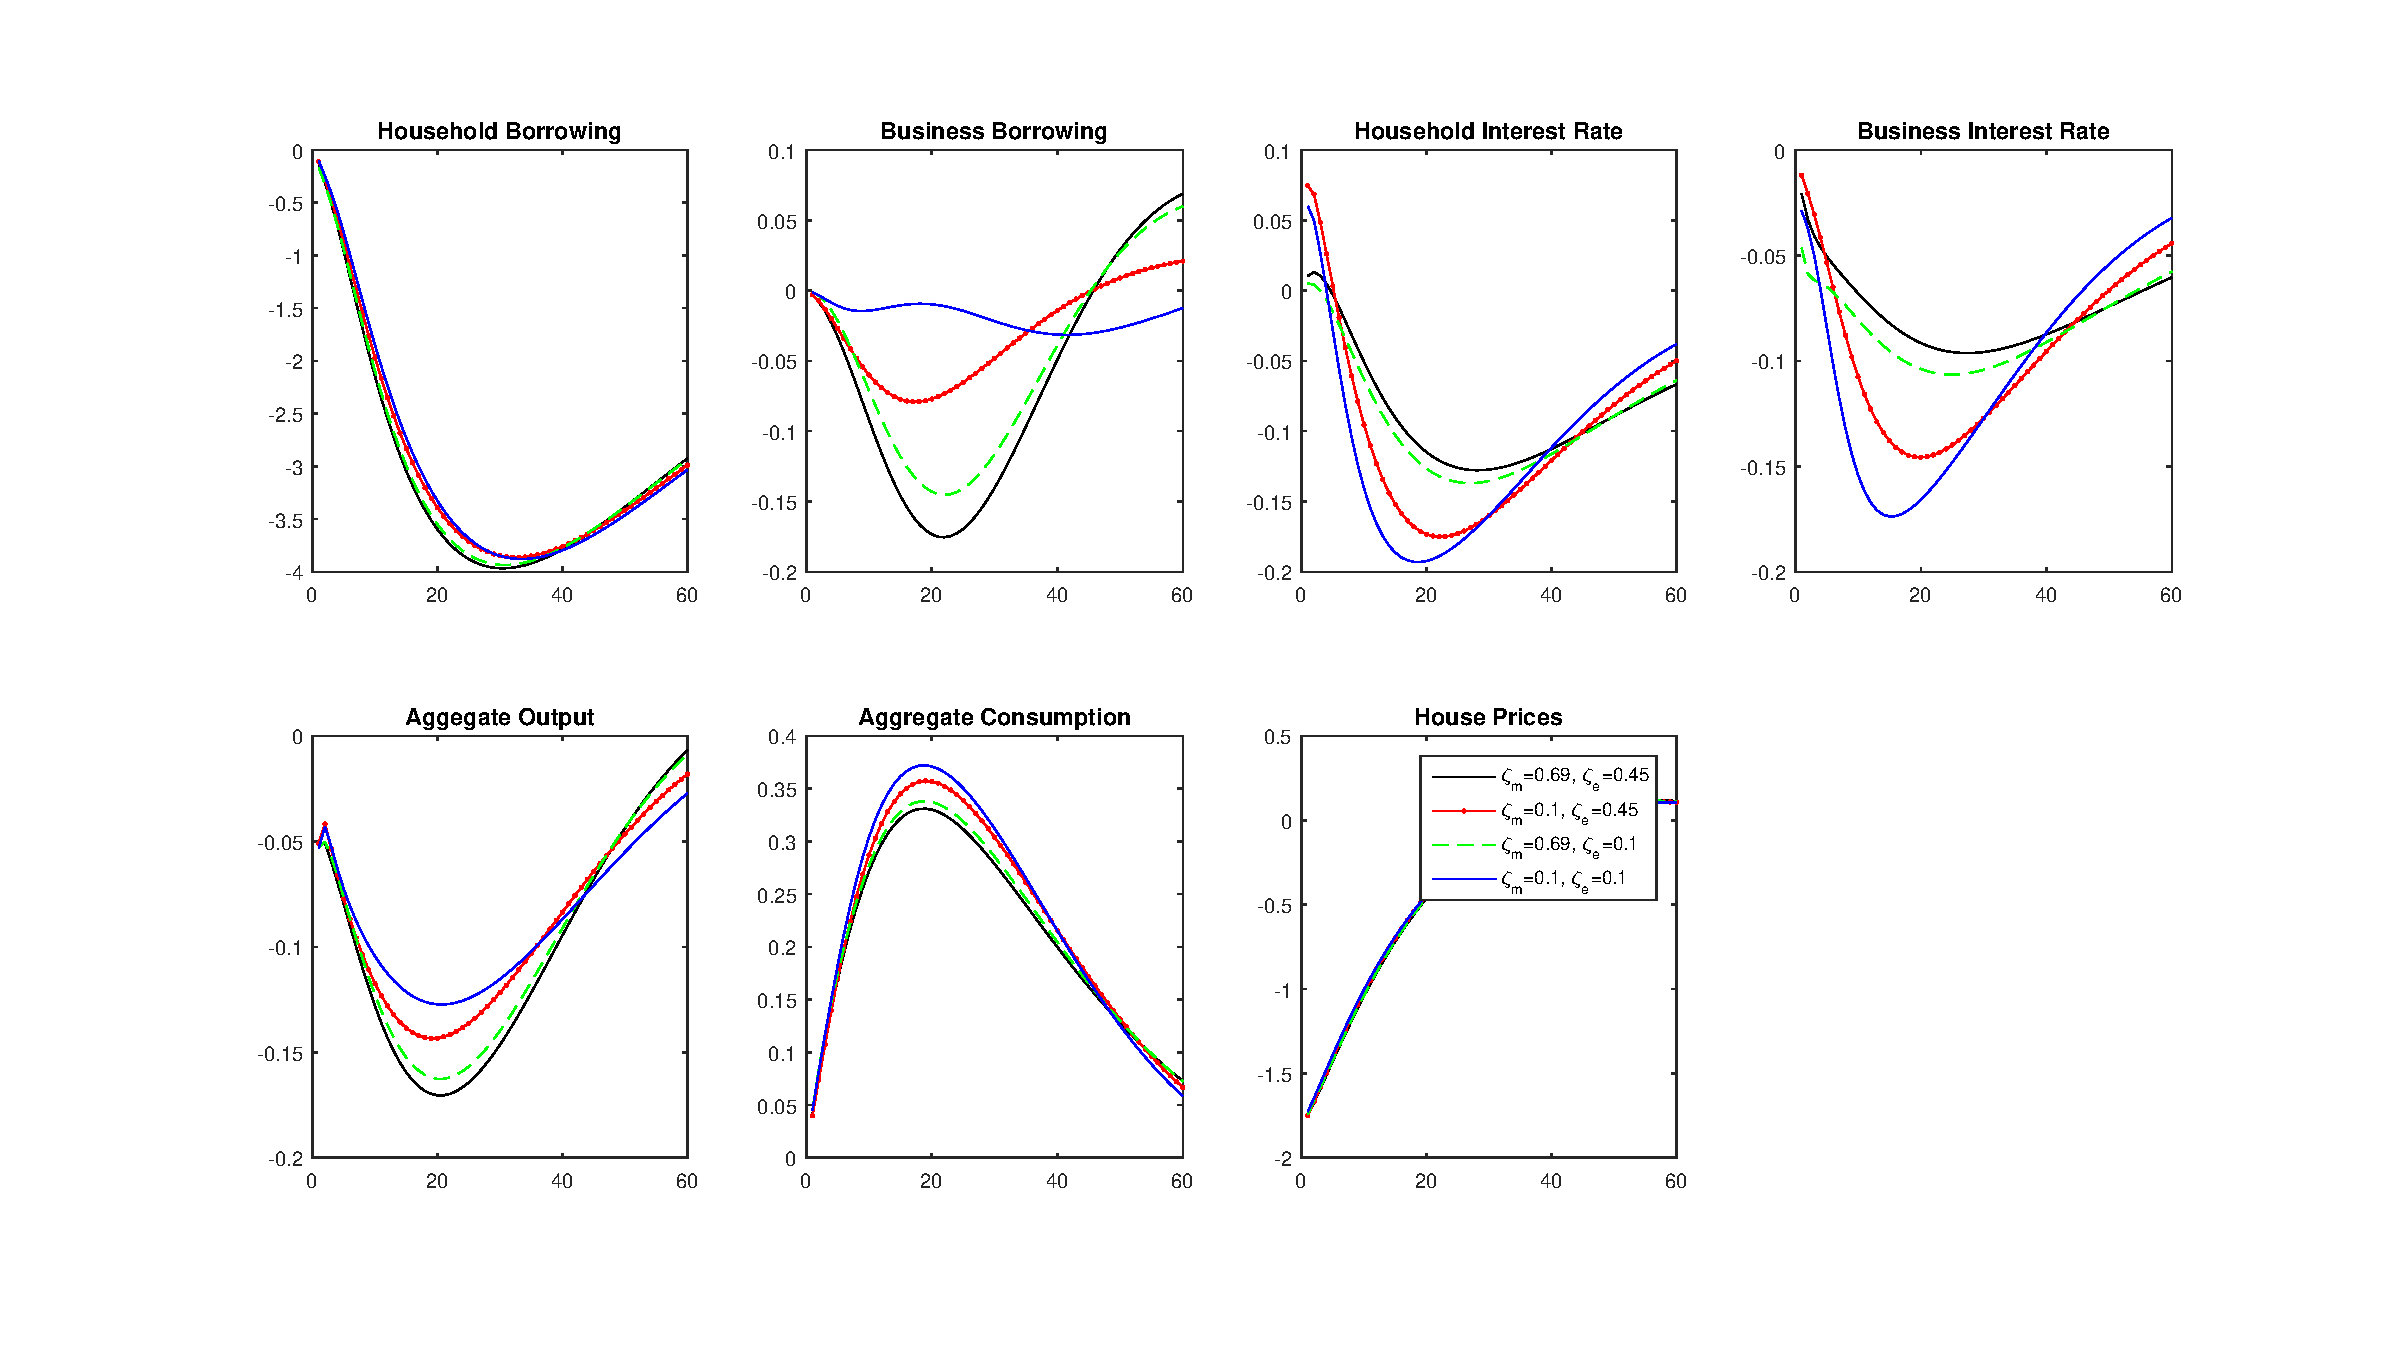
\includegraphics[scale=0.45]{stickinessJ.pdf}
\end{figure}

%\begin{figure}[H]
%\centering
%\caption{Positive Housing Depreciation Shock}
%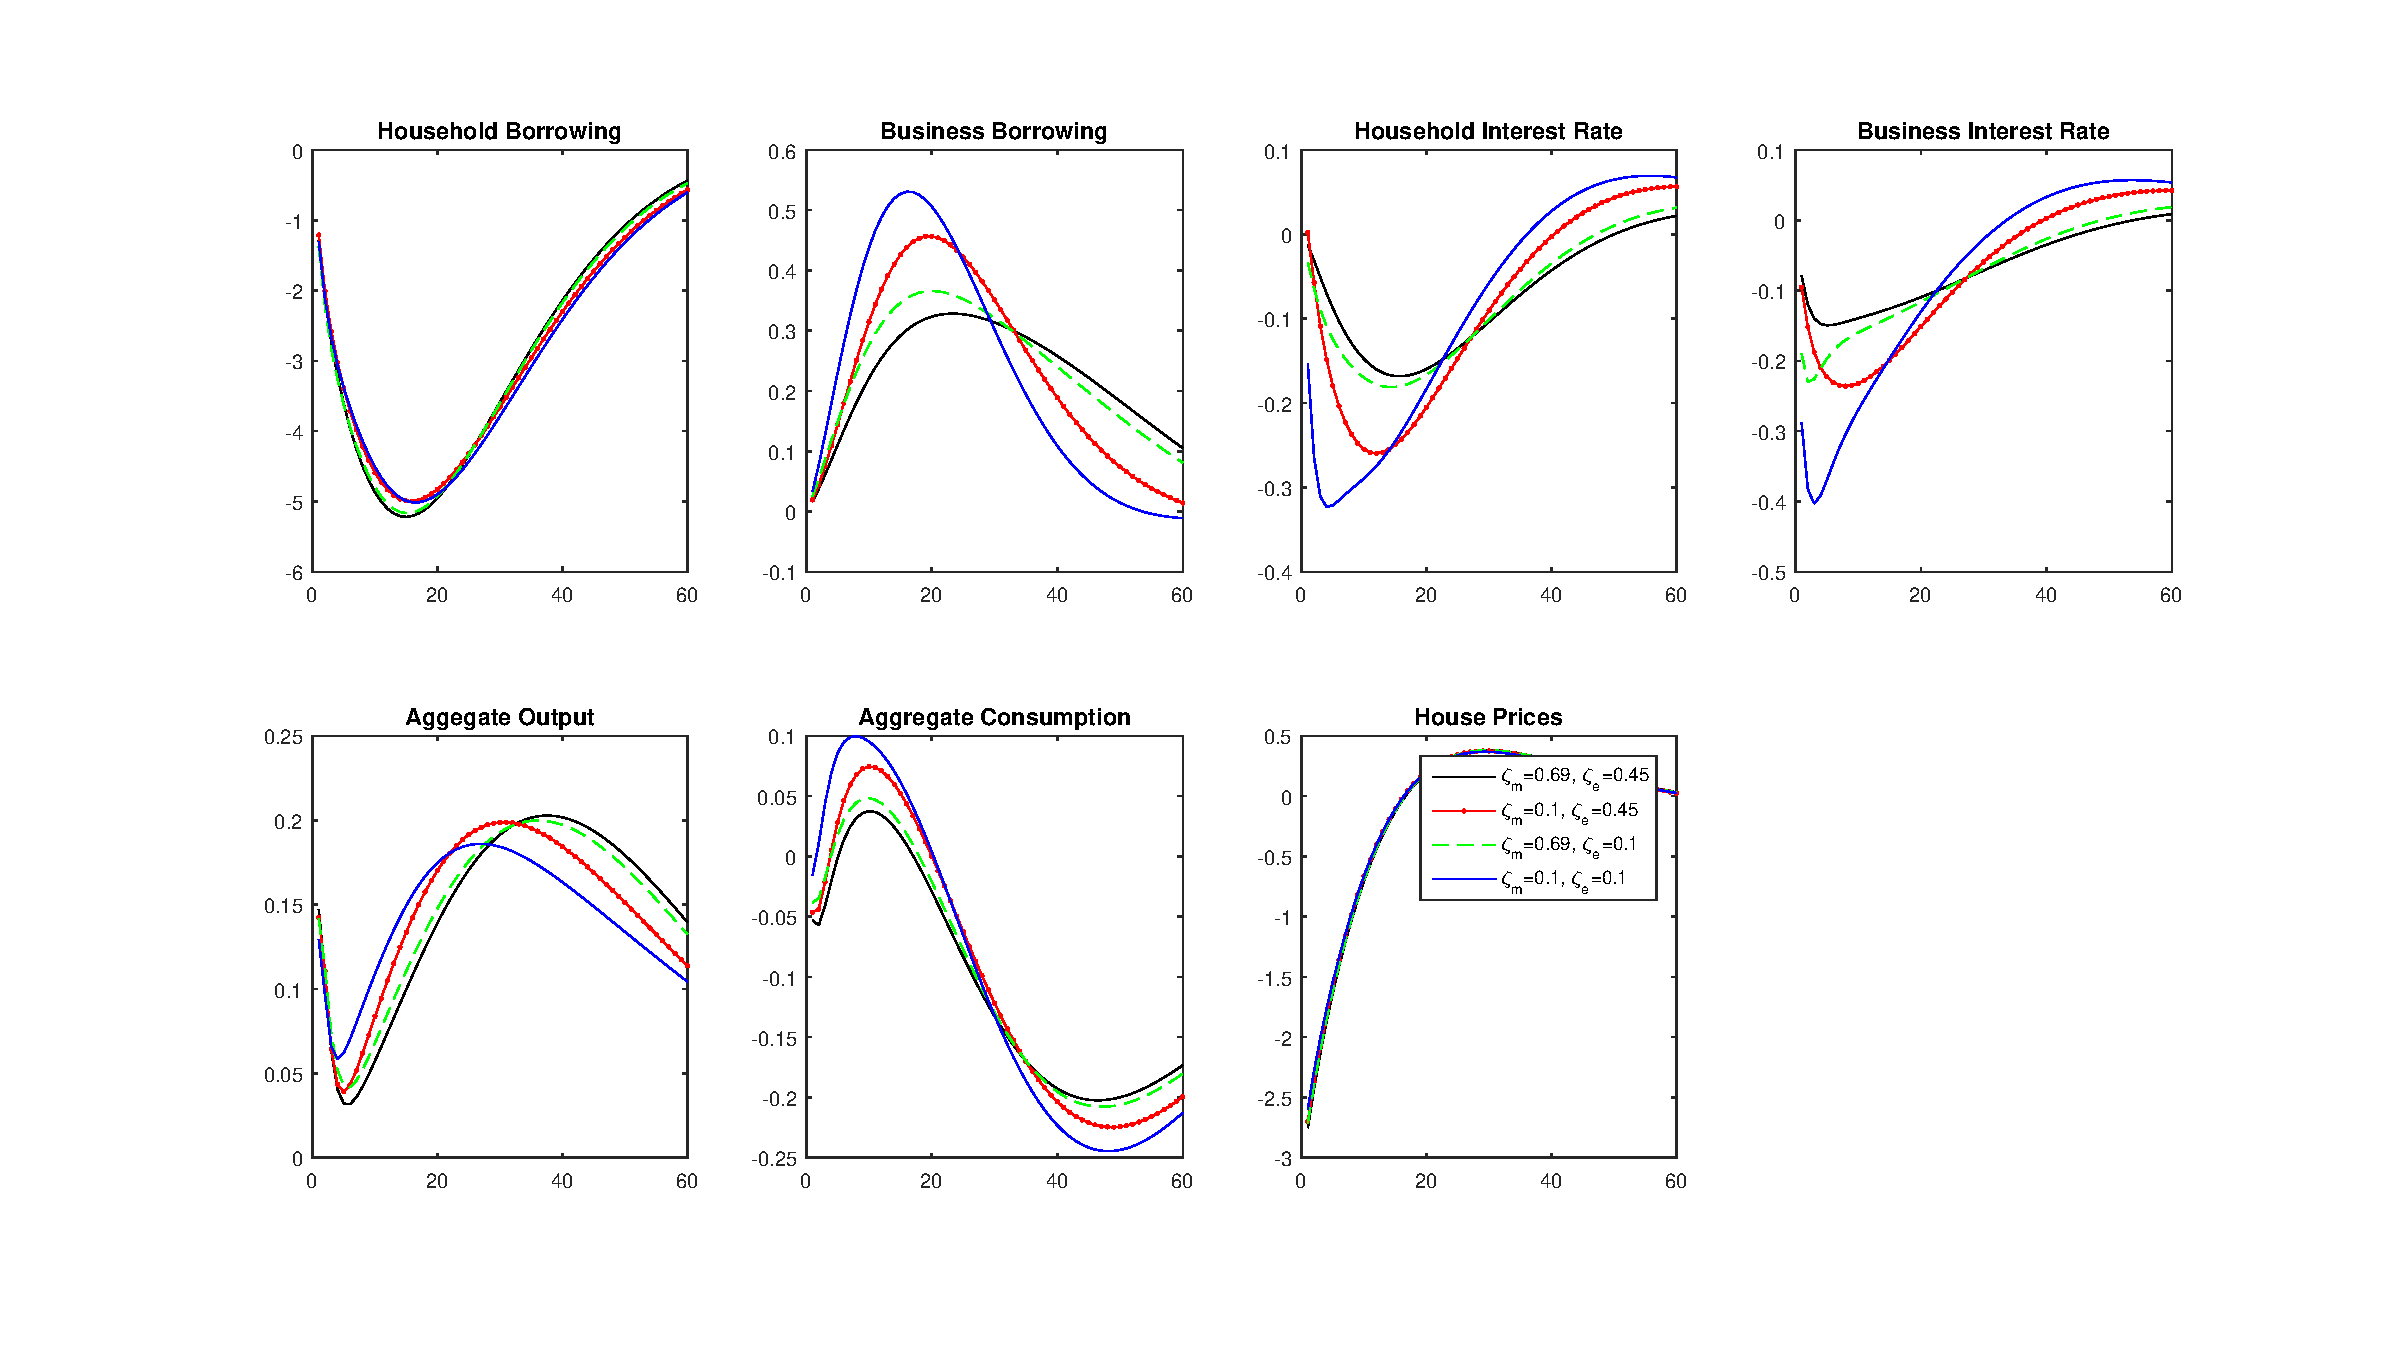
\includegraphics[scale=0.5]{stickinessHd.pdf}
%\end{figure}



\begin{figure}[H]
\centering
\caption{Positive Capital Depreciation Shock}
\label{stickinessHk_figure}
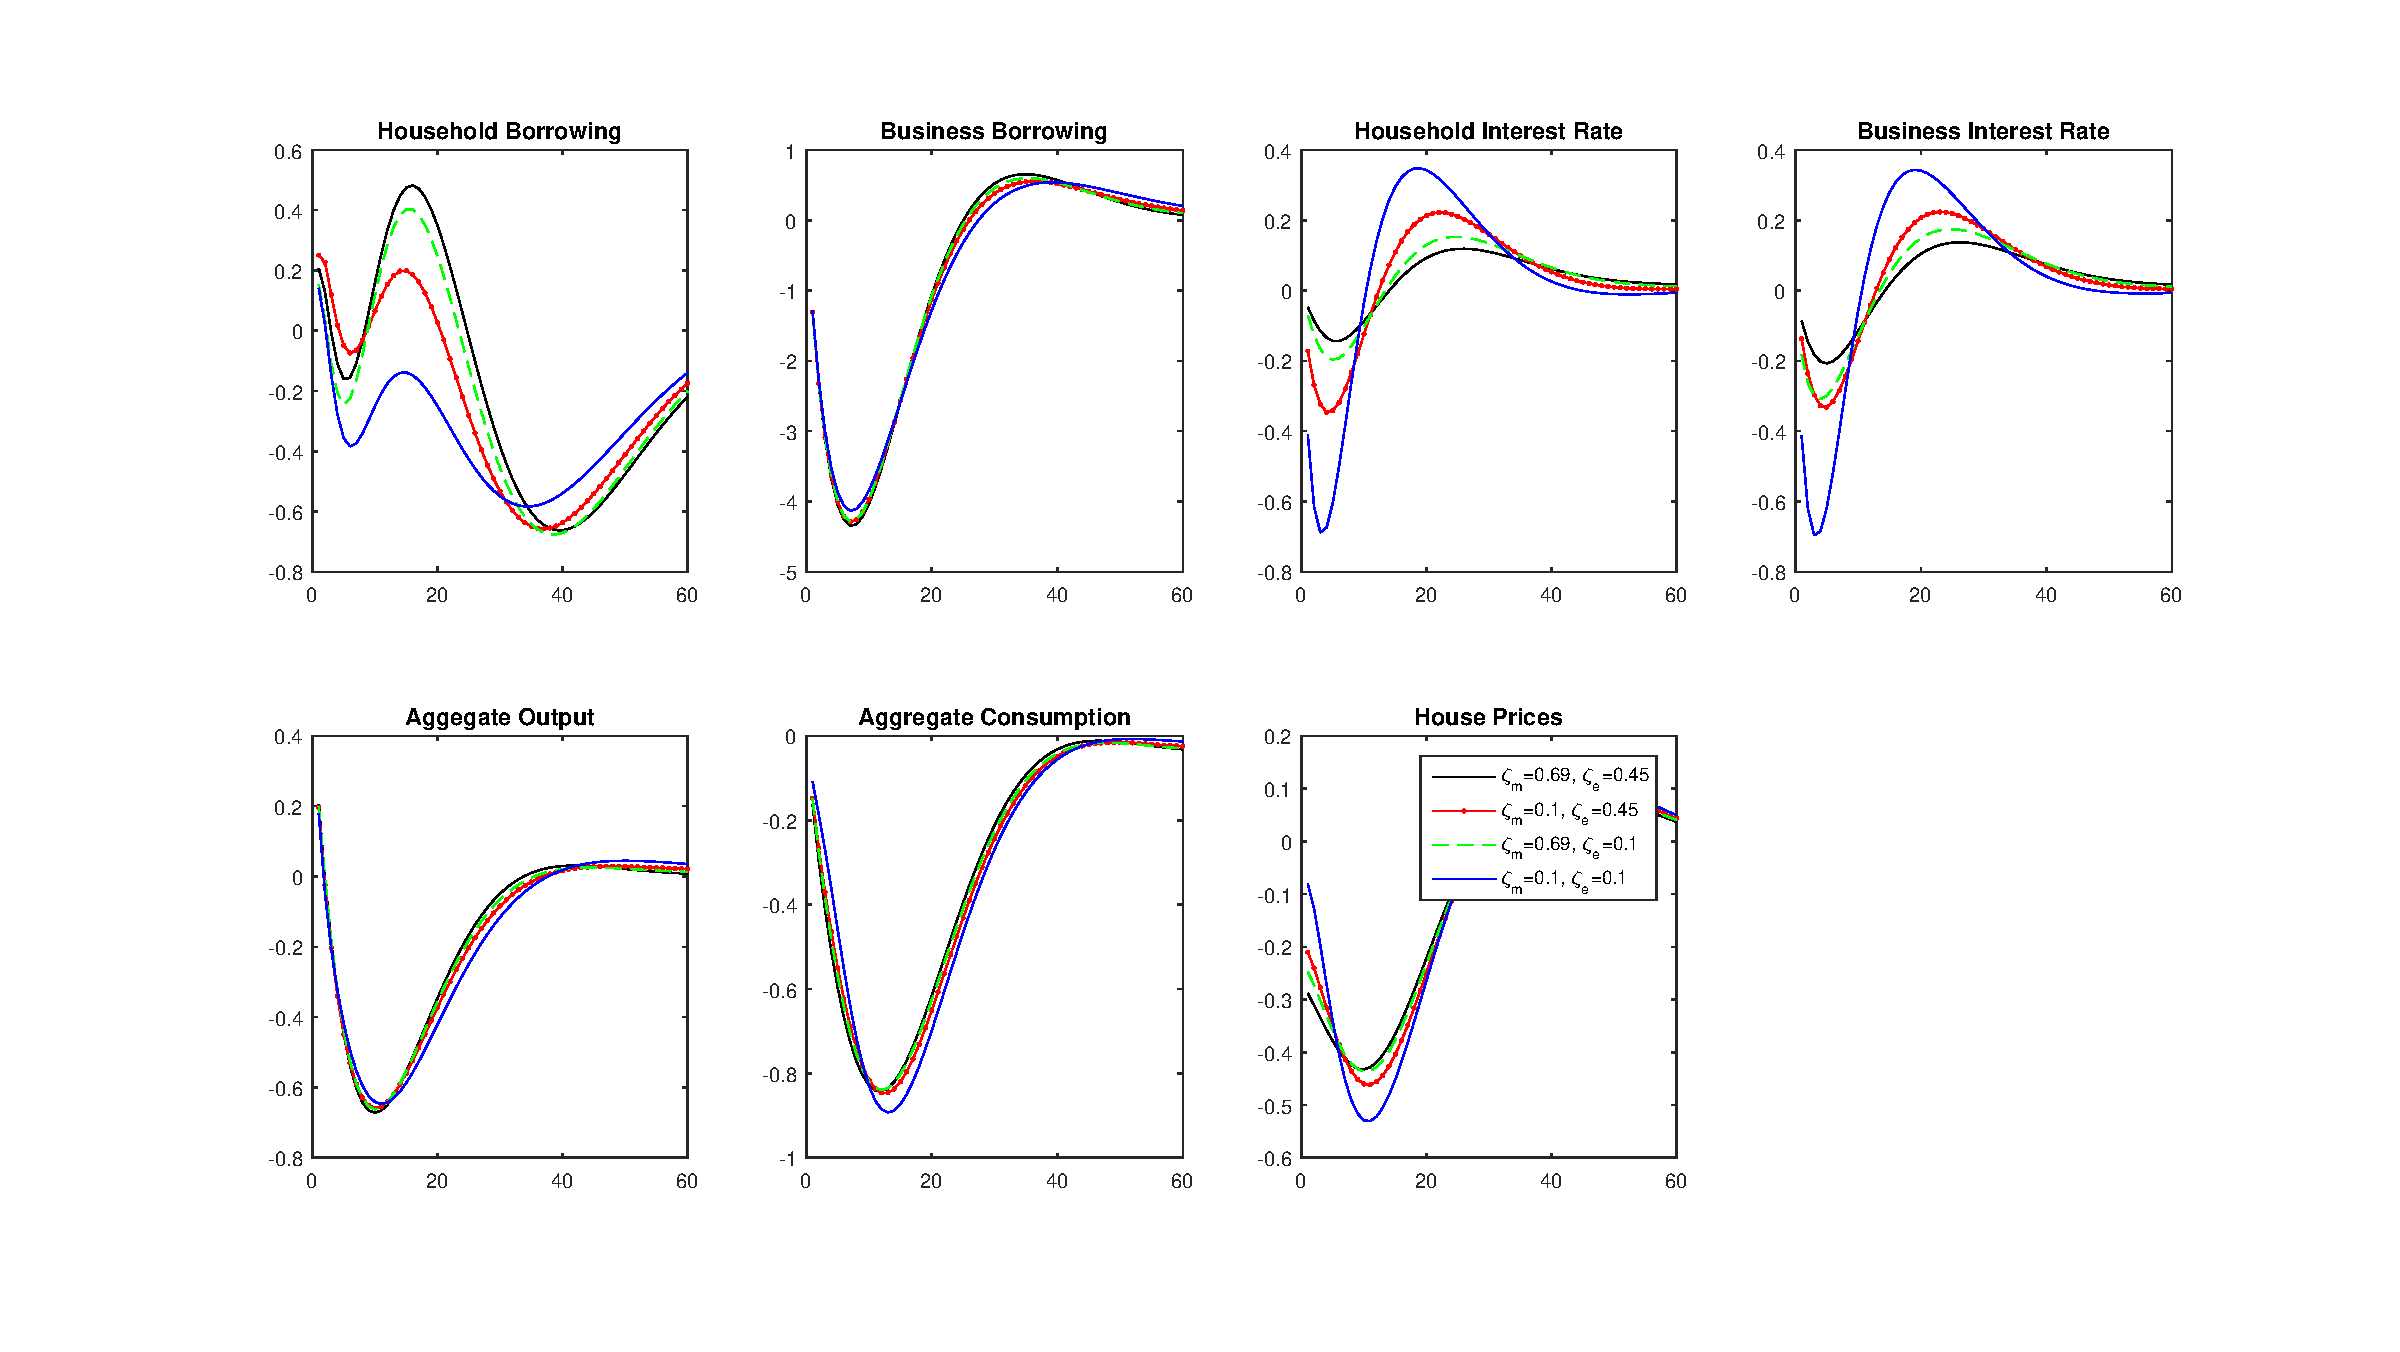
\includegraphics[scale=0.5]{stickinessHk.pdf}
\end{figure}

\begin{figure}[H]
\centering
\caption{Negative Bank Capital Shock}
\label{stickinessCAB_figure}
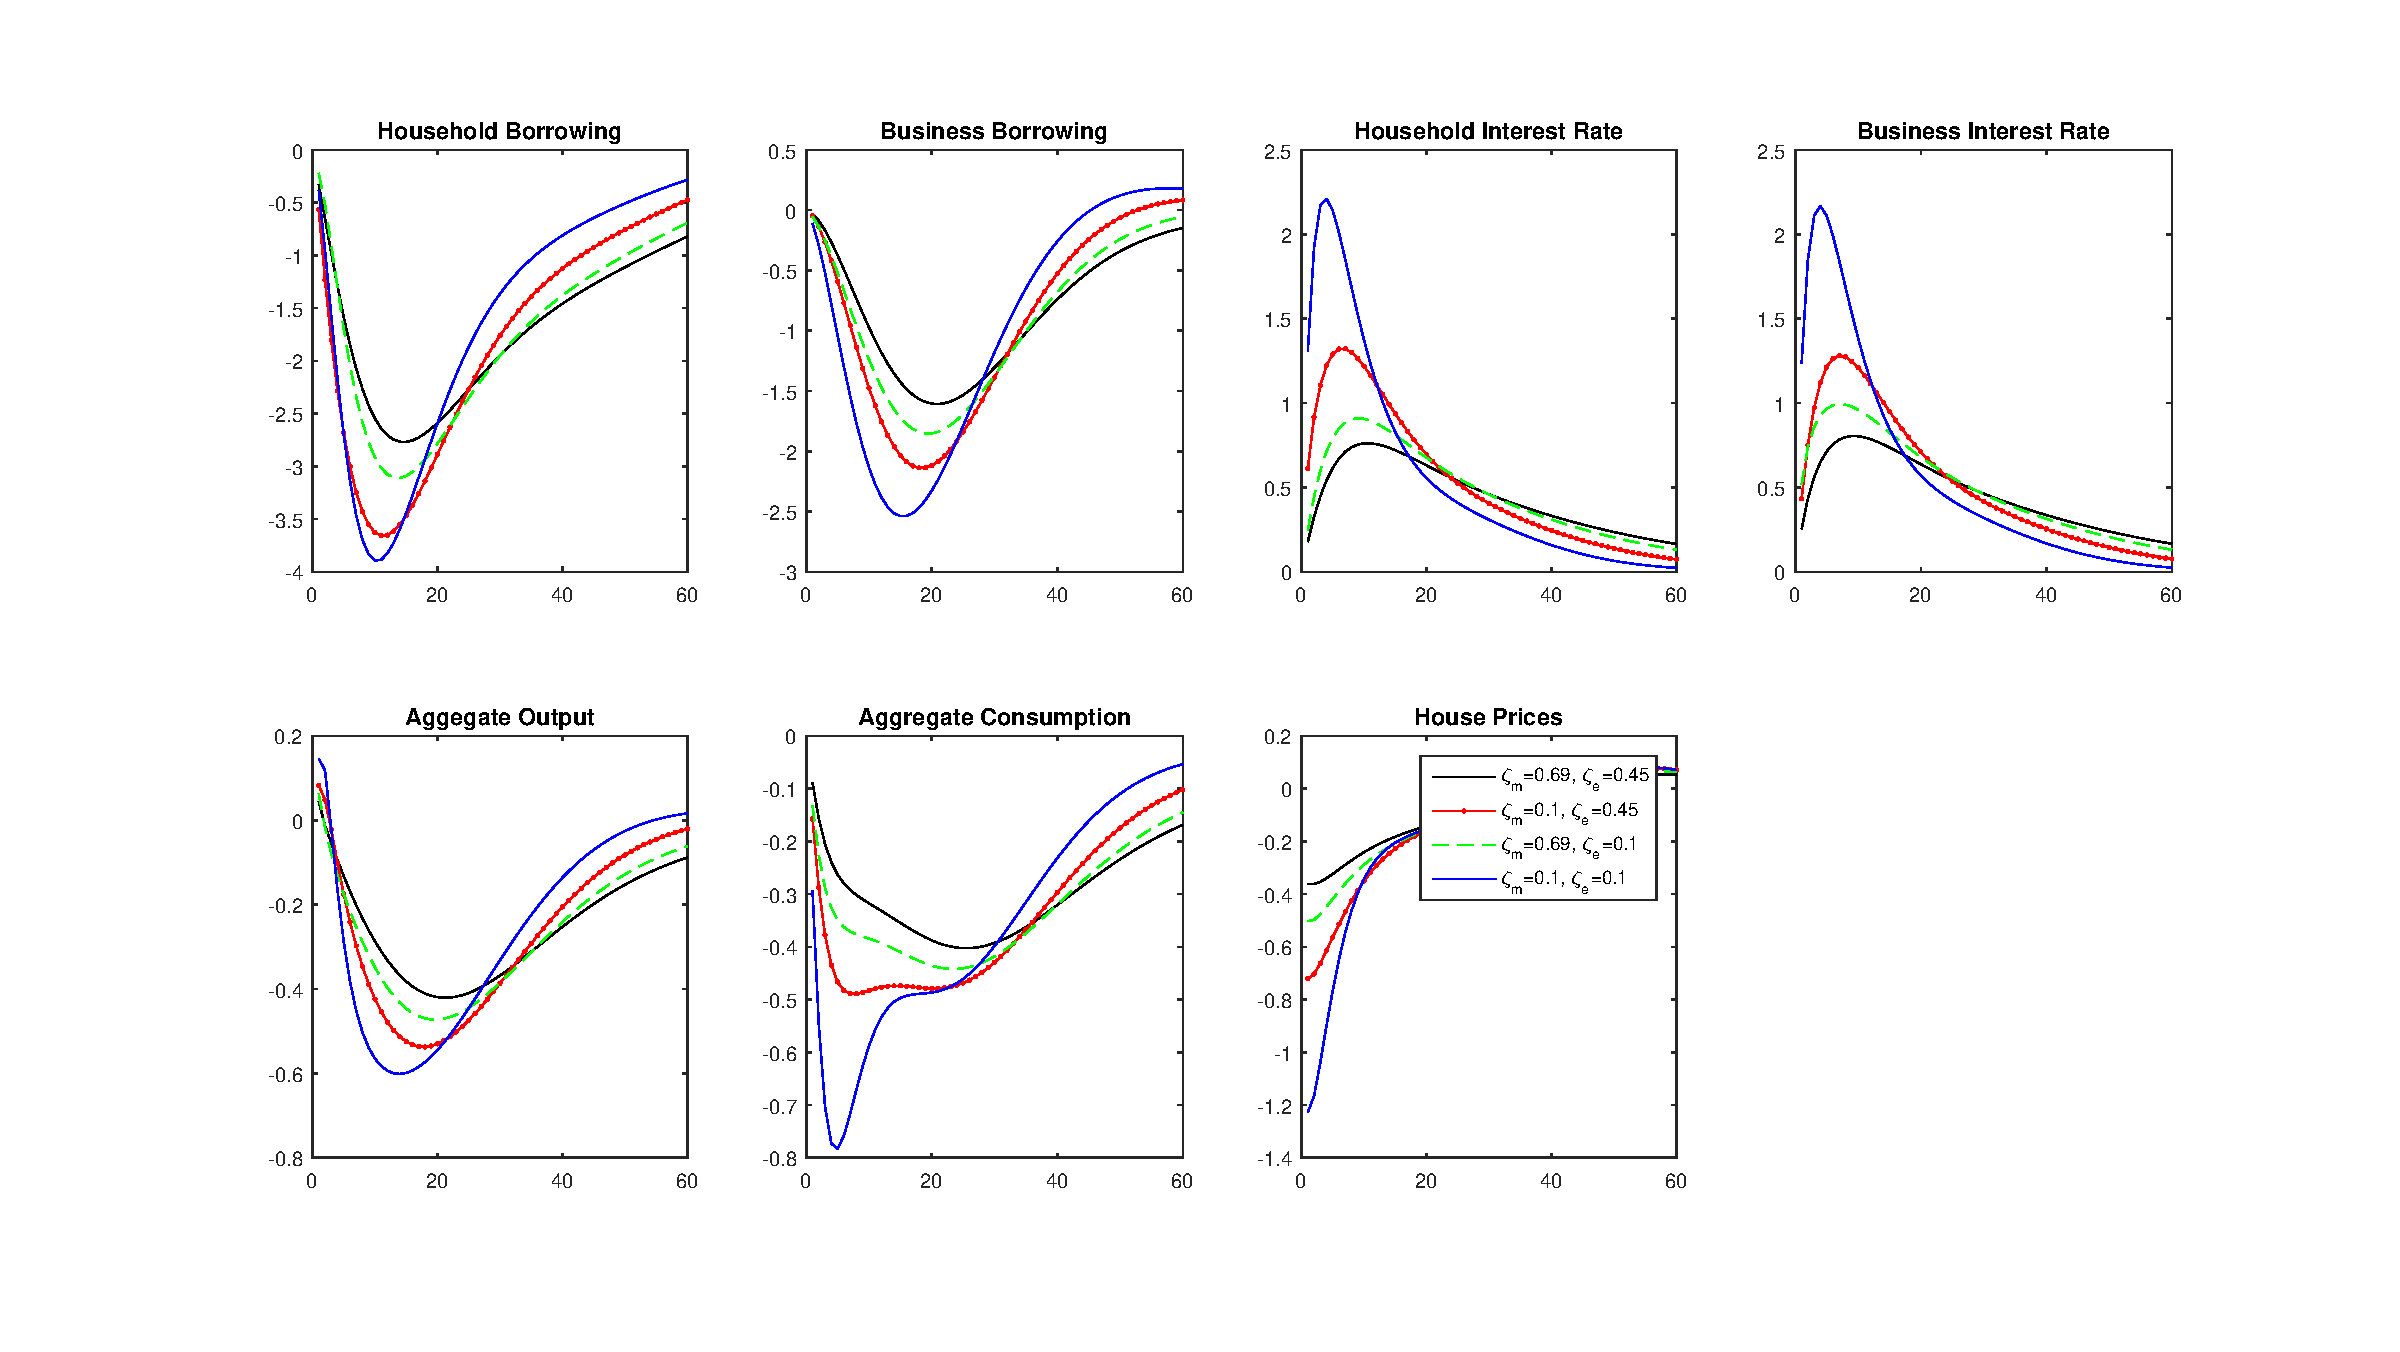
\includegraphics[scale=0.5]{stickinessCAB.pdf}
\end{figure}




\begin{table}[h]
\caption{Does CcyB improve things when SCRs are at their baseline value? }
\label{impact_ccyb_table}
\begin{tabular}{l|l|l}
\small
Variable & \% Change in Level & \% Change in Volatility \\
\hline
Baseline SCR+LTV & & \\
\hline
    Corporate Credit           &       0.007    &      0.042 \\
    Mortgage Credit            &      0.003    &       0.029 \\
    Output         &     0.0019    &    0.37 \\ 
    Household Welfare       &     0.003     &     -0.002\\
  
 \hline
No Interest Stickiness & & \\
\hline

    Corporate Credit           &       0.016    &      0.072 \\
    Mortgage Credit            &      0.008    &       0.108 \\
    Output         &     0.005    &    0.675 \\ 
    Household Welfare       &     0.013     &     -0.009\\
  \end{tabular}
\end{table}



\newpage


\section*{Stickiness \& Prudential Policy Interactions}
%preference shock looks weird here--> larger effects with higher capital requirements or with CCyB and the second
%order effects dominate everything


%figure 14 CCyB: check what happens to bank capital with bank capital shock



In this section, we assess how prudential policies affect the propagation of different shocks, and how staggered interest rates influence the transmission of these shocks. Figure 13 shows the effect of a positive housing depreciation shock on mortgage and corporate lending, both for the estimated degree of interest rate stickiness and for the case with low interest rate stickiness\footnote{We set the the interest rate stickiness to 0.1 in both sectors for the low stickiness case.}. Panel (c) compares the impulse response functions for a capital adequacy ratio (CAR) of 15\% and 11\%.  The overall fall in mortgage lending is about 5\% at its trough in all four cases, but is somewhat more pronounced when the CAR ratio is higher. [WHY?] Due to substitution effects, corporate lending increases, but less in absolute terms compared with the fall in mortgage lending. If interest rates are sticky, banks cannot reduce the corporate lending rate quickly, so the increase in corporate lending is lower at its peak but continues for longer. A higher CAR reduces the increase in corporate lending for both degrees of interest rate stickiness. [WHY?] Overall, the cumulative difference between the case of high and low interest rate is 3.2\% for mortgage lending and 0.4\% for corporate lending [IS THIS FOR HIGH OR LOW CAR?].

The pattern is similar when we analyse the CCyB instead of CAR (Panel a). [NEED EXPLAIN WHY NO DIFFERENCE FOR MORTGAGES, BUT SIMILAR PATTERN FOR CORPORATES.]

In panel b, the path of corporate lending is unaffected by different settings of the LTV ratio, in contrast with the capital-based instruments.

Figure 14 shows a shock that increases capital depreciation. As expected, corporate lending decreases in all three cases, by about 4\%. The shock gets propagated to the mortgage sector, where lending decreases by more if interest rates are more flexible (the fluctuations stem from second round effects where a reduced capital stock impacts the overall economy negatively, which occur on top of banks substituting mortgage for corporate lending). The impact of policy tools is relatively small in this case.

In contrast to the previous two shocks, a negative bank capital shock (Figure 15) affects both sectors more equally, with mortgage lending falling by up to 5\%, and corporate lending by up to 2.5\%. The higher effect on mortgage lending is due to [x]. Panel a shows that a higher CAR substantially reduces the subsequent fall in lending after a shock to bank capital. Mitigating banks’ deleveraging after a negative shock to their capital was one of the main aims of higher minimum capital requirements in the aftermath of the financial crisis. Our results suggest that higher CARs achieve this objective. A higher degree of interest rate stickiness prevents banks from increasing their lending rates quickly as a response to the shock, so lending falls by less compared with a case of flexibles interest rates – though the adjustment is spread out over a longer time horizon.

The CCyB has almost no effect (panel a) because of […].

Panel b reveals that the fall in lending (for both a high and low degree of interest rate stickiness) is more severe if households are more leveraged: [WHY?]

 

 

[NEED TO WORK IN THESE CUMULATIVE DIFFERENCES]

[SOME SORT OF SUMMARY, MAYBE IN TABLE FORMAT?]

In summary, the above figures show that the impact of macroprudential tools will generally be weaker in cases where interest rate stickiness is high. The type of shock matters for the impact of prudential tools on the transmission of the shock: […]


\footnote{We calculate te cumulative difference as follows: first, the cumulative impact of a macroprudential tool is calculated as the area between  the impulse responses for two given values of that tool. We repeat this calculation for the cases with and without interest rate stickiness, and consider the difference between the two as our measure of the cumulative difference}. 

%\begin{figure}[h]
%\caption{Negative housing preference shock. Cumulative difference calculated as the  }
%\subfigure[]{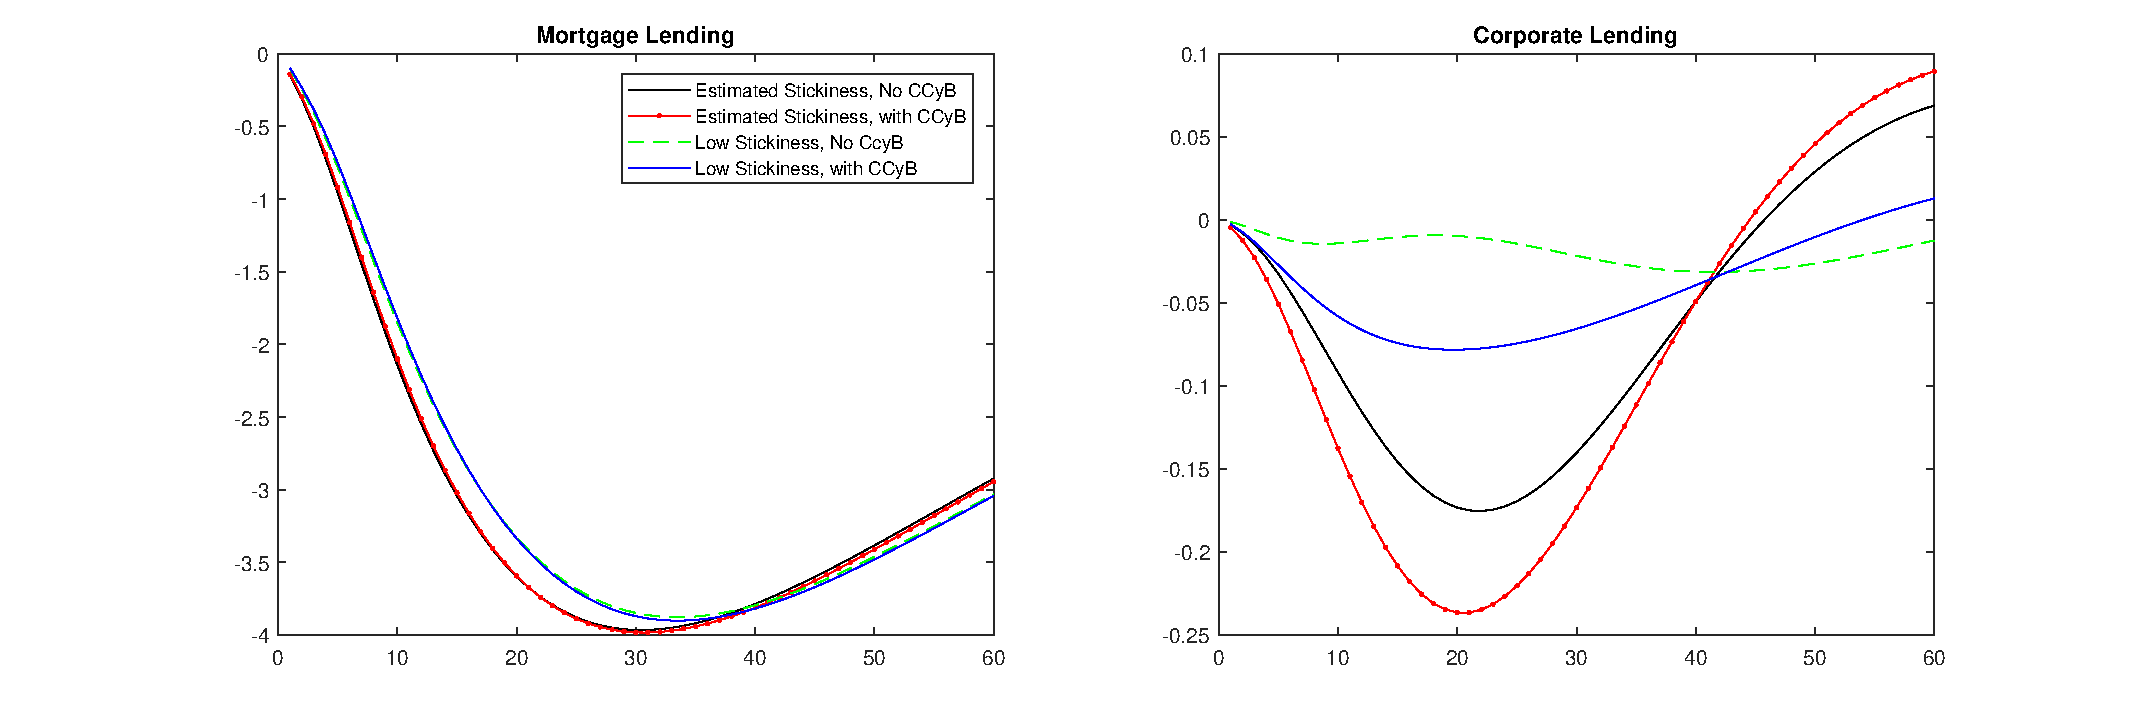
\includegraphics[scale=0.5]{stickiness_ccybJ.pdf}}
%\subfigure[]{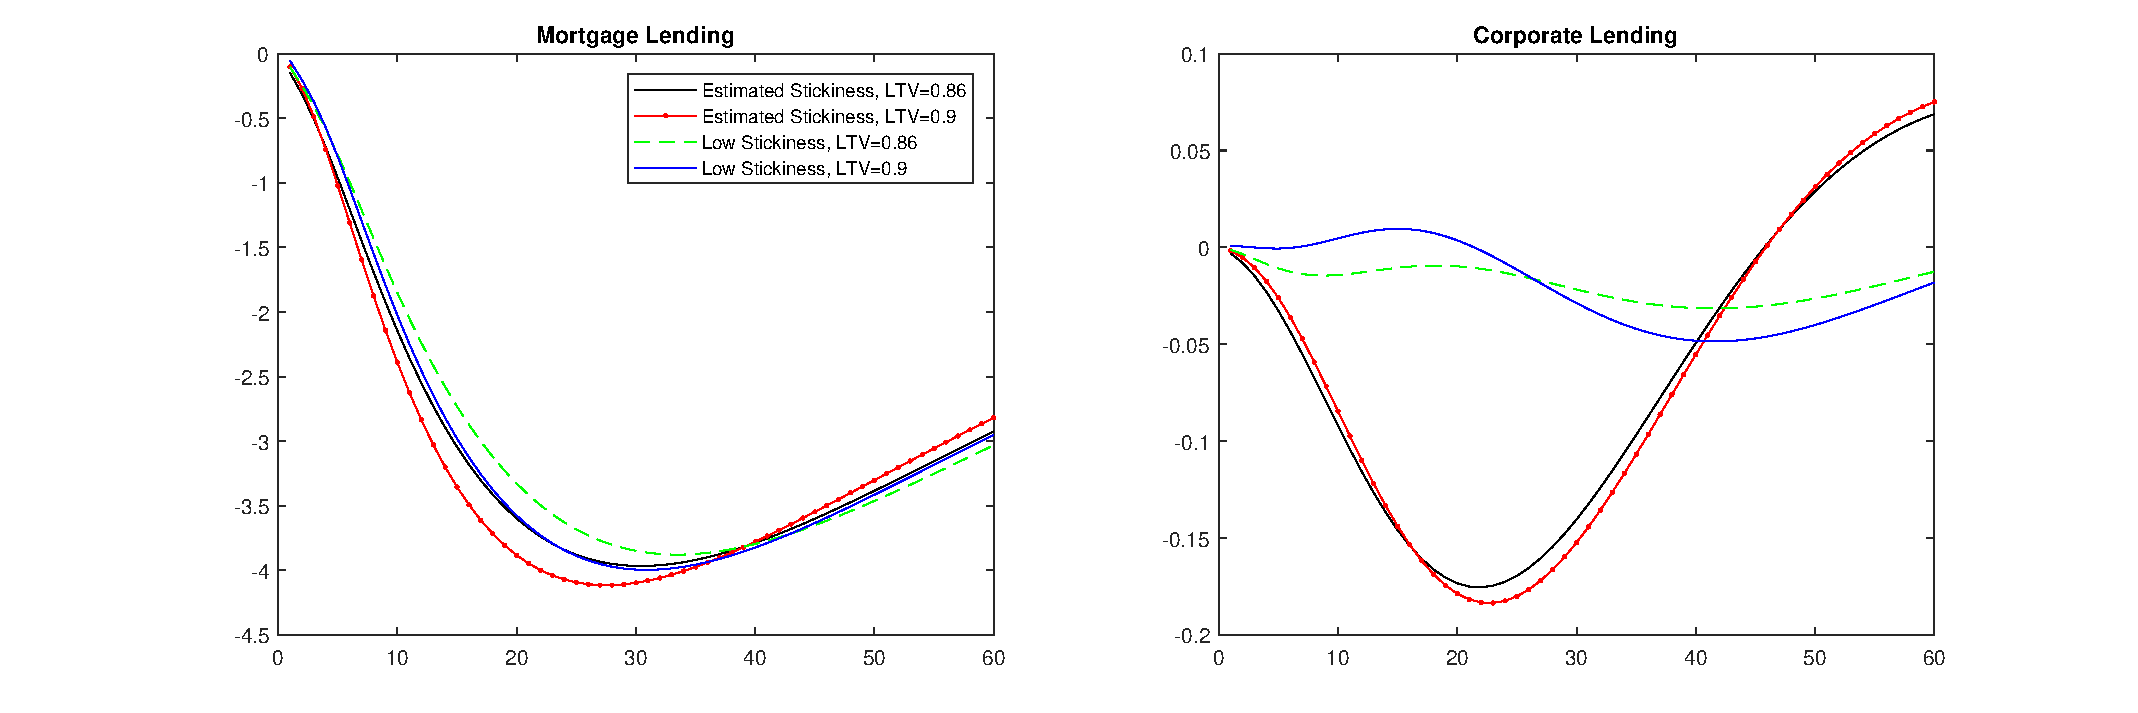
\includegraphics[scale=0.5]{stickiness_LTVJ.pdf}}
%\subfigure[]{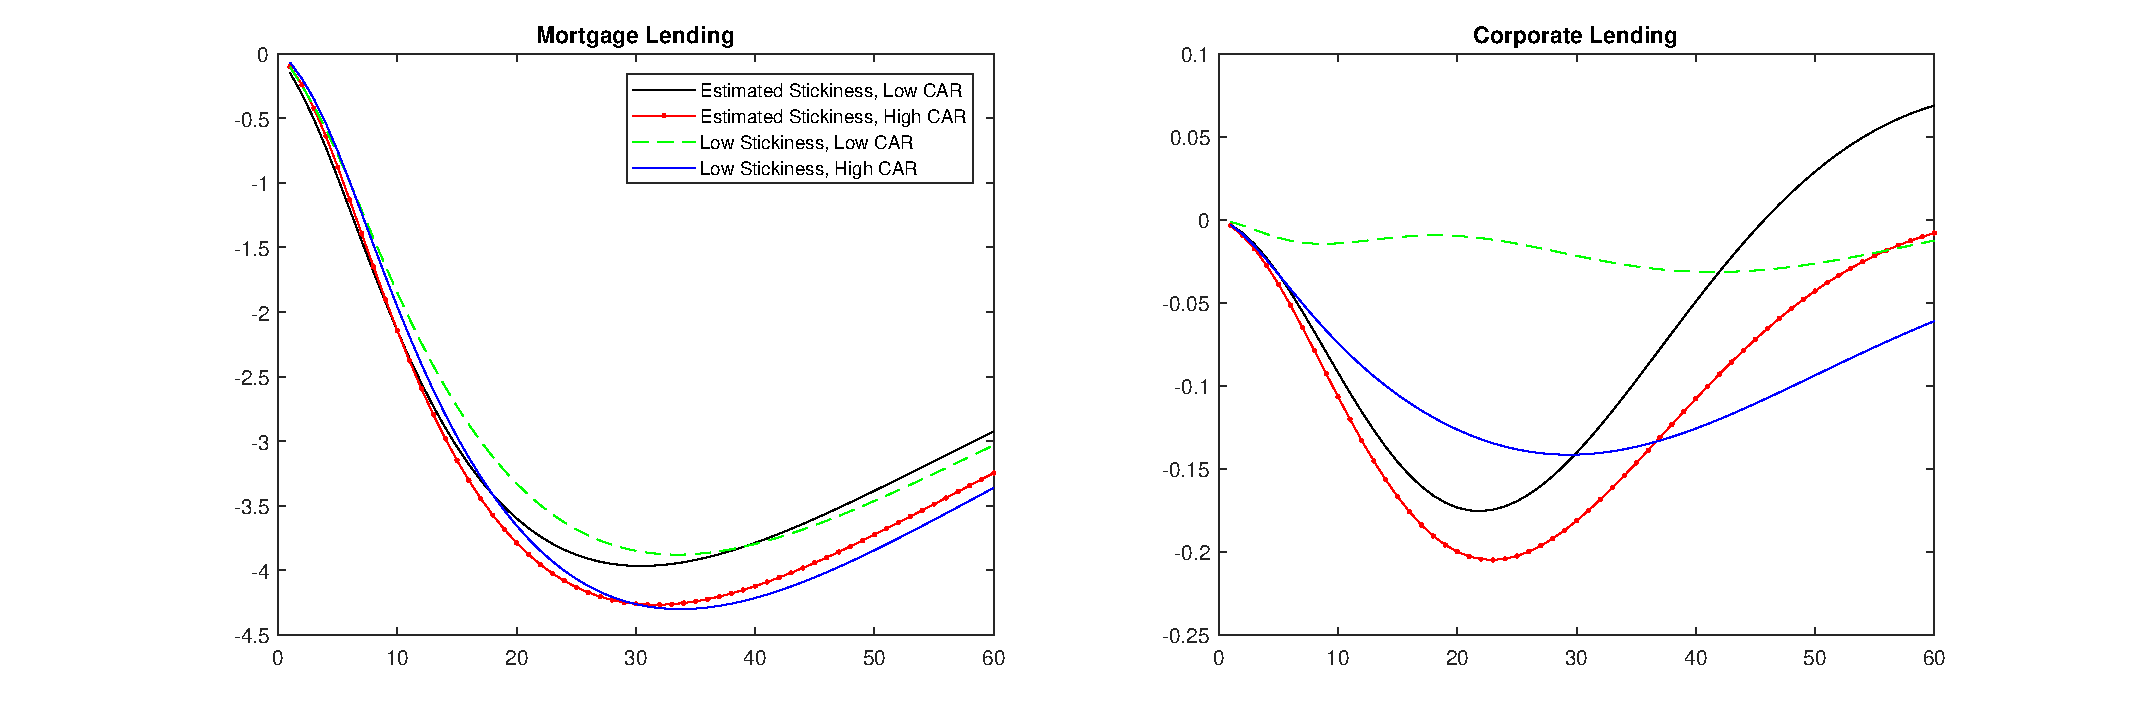
\includegraphics[scale=0.5]{stickiness_CARJ.pdf}}
%\end{figure}

\begin{figure}[H]

\caption{Positive housing depreciation shock.  }
\label{stickinessHd_pru_figure}
\subfigure[Cumulative differences: 0.14 \% and 0.59 \%.]{\includegraphics[scale=0.45]{stickiness_ccybHd.pdf}}
\subfigure[Cumulative differences: -2.13 \% and 0.17 \%.]{\includegraphics[scale=0.45]{stickiness_LTVHd.pdf}}
\subfigure[Cumulative differences: 3.23 \% and 0.38 \%.]{\includegraphics[scale=0.45]{stickiness_CARHd.pdf}}
\end{figure}

\begin{figure}[H]
\caption{Positive capital depreciation shock.  }
\label{stickinessHk_pru_figure}
\subfigure[Cumulative differences: 4.6 \% and 1.44 \%.]{\includegraphics[scale=0.45]{stickiness_ccybHk.pdf}}
\subfigure[Cumulative differences: 0.07 \% and 0.2 \%.]{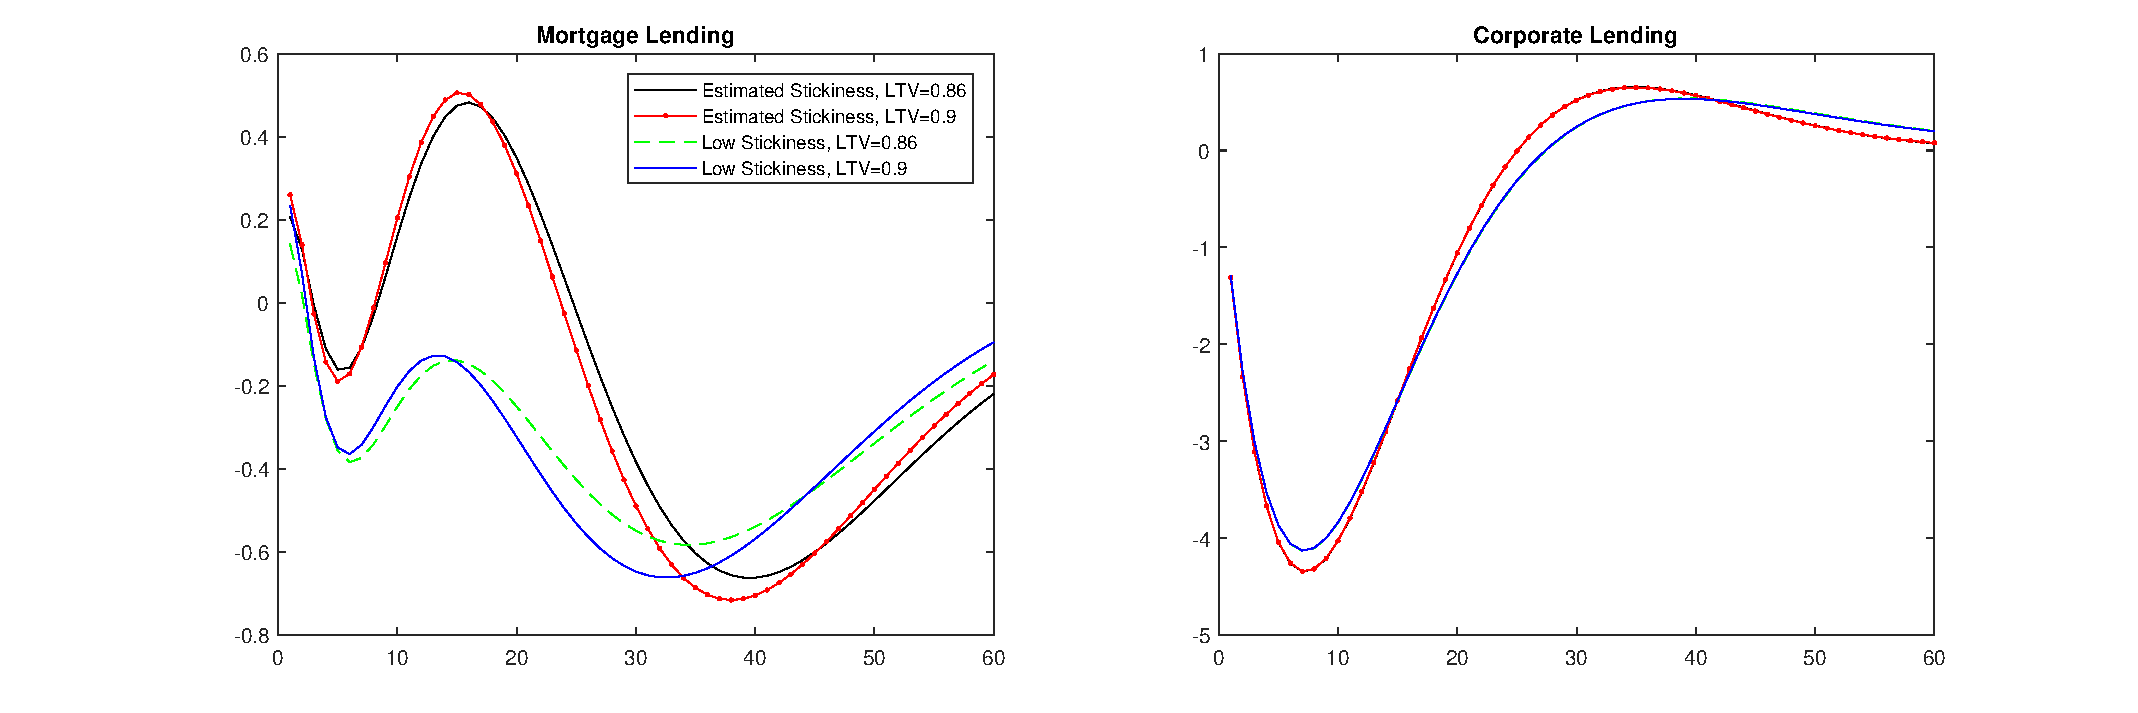
\includegraphics[scale=0.45]{stickiness_LTVHk.pdf}}
\subfigure[Cumulative differences: 1.55 \% and 0.16 \%.]{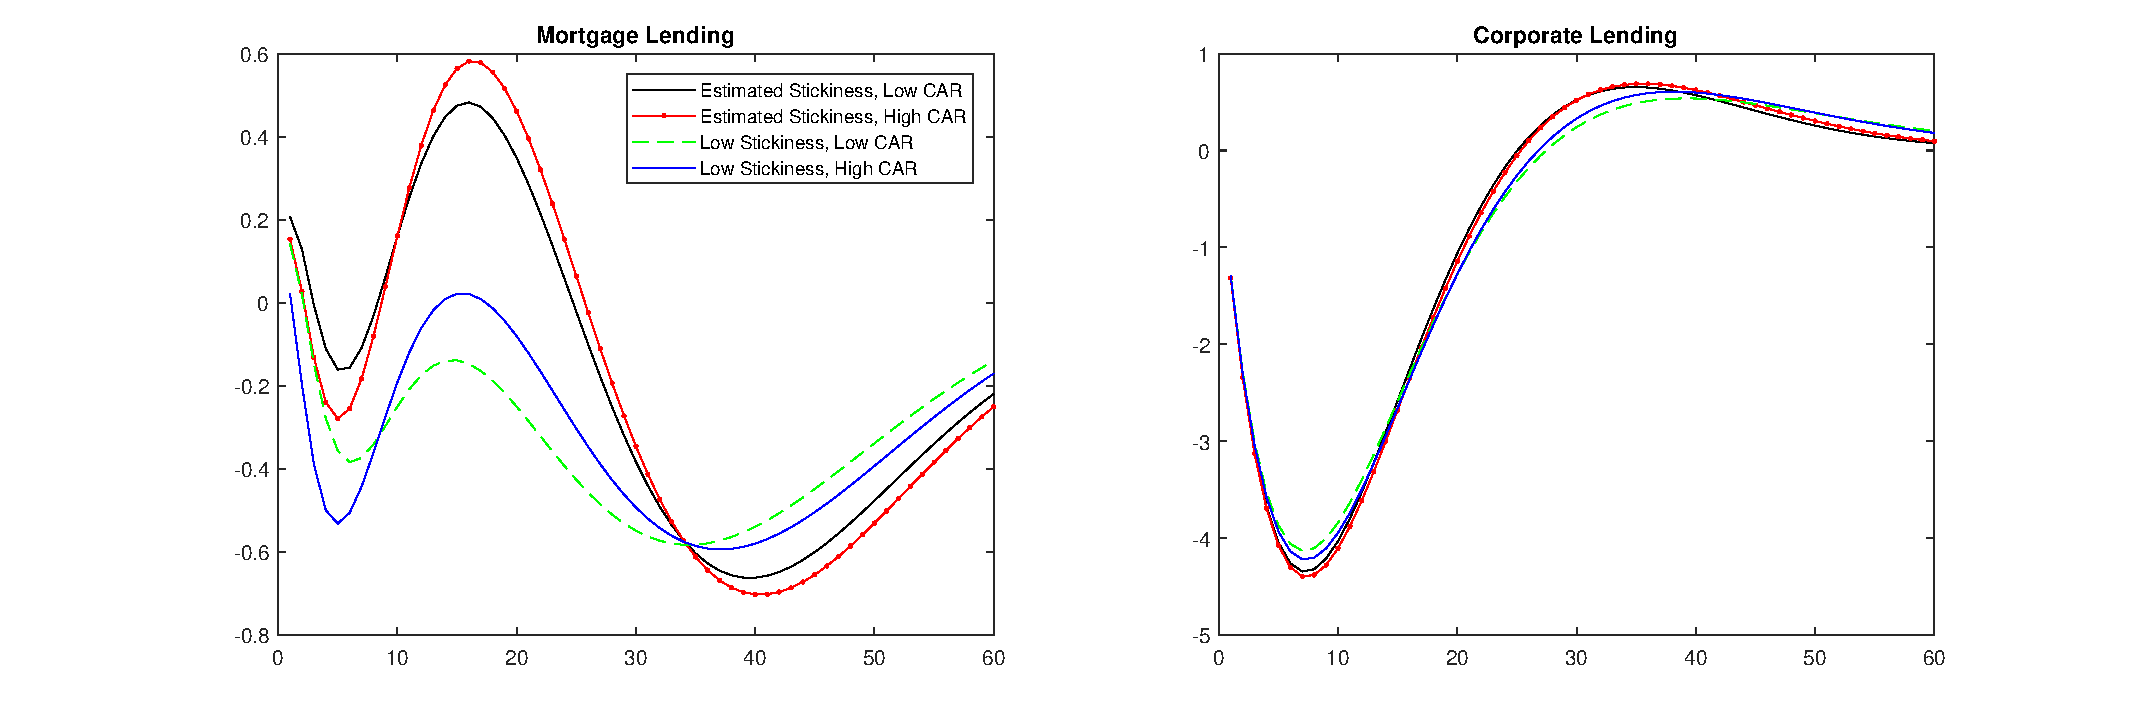
\includegraphics[scale=0.45]{stickiness_CARHk.pdf}}
\end{figure}




\begin{figure}[H]
\caption{Negative bank capital shock.}
\label{stickinessCAB_pru_figure}
\subfigure[Cumulative differences: 2.54 \% and 1.4 \%.]{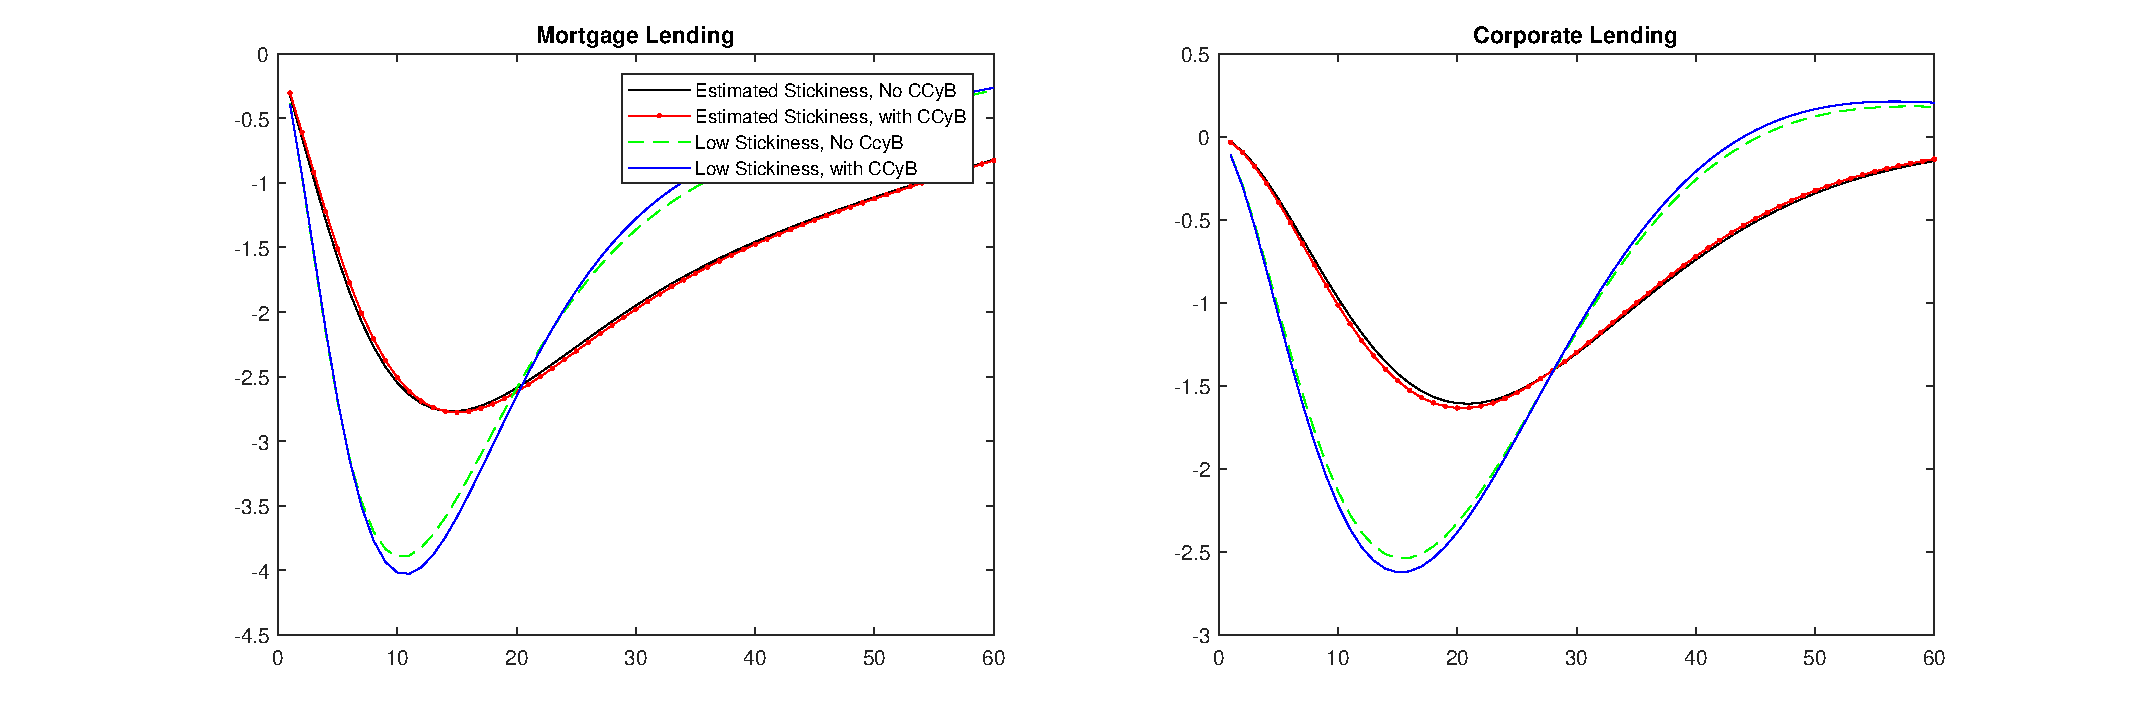
\includegraphics[scale=0.45]{stickiness_ccybECAB.pdf}}
\subfigure[Cumulative differences: 3.73 \% and 0.69 \%.]{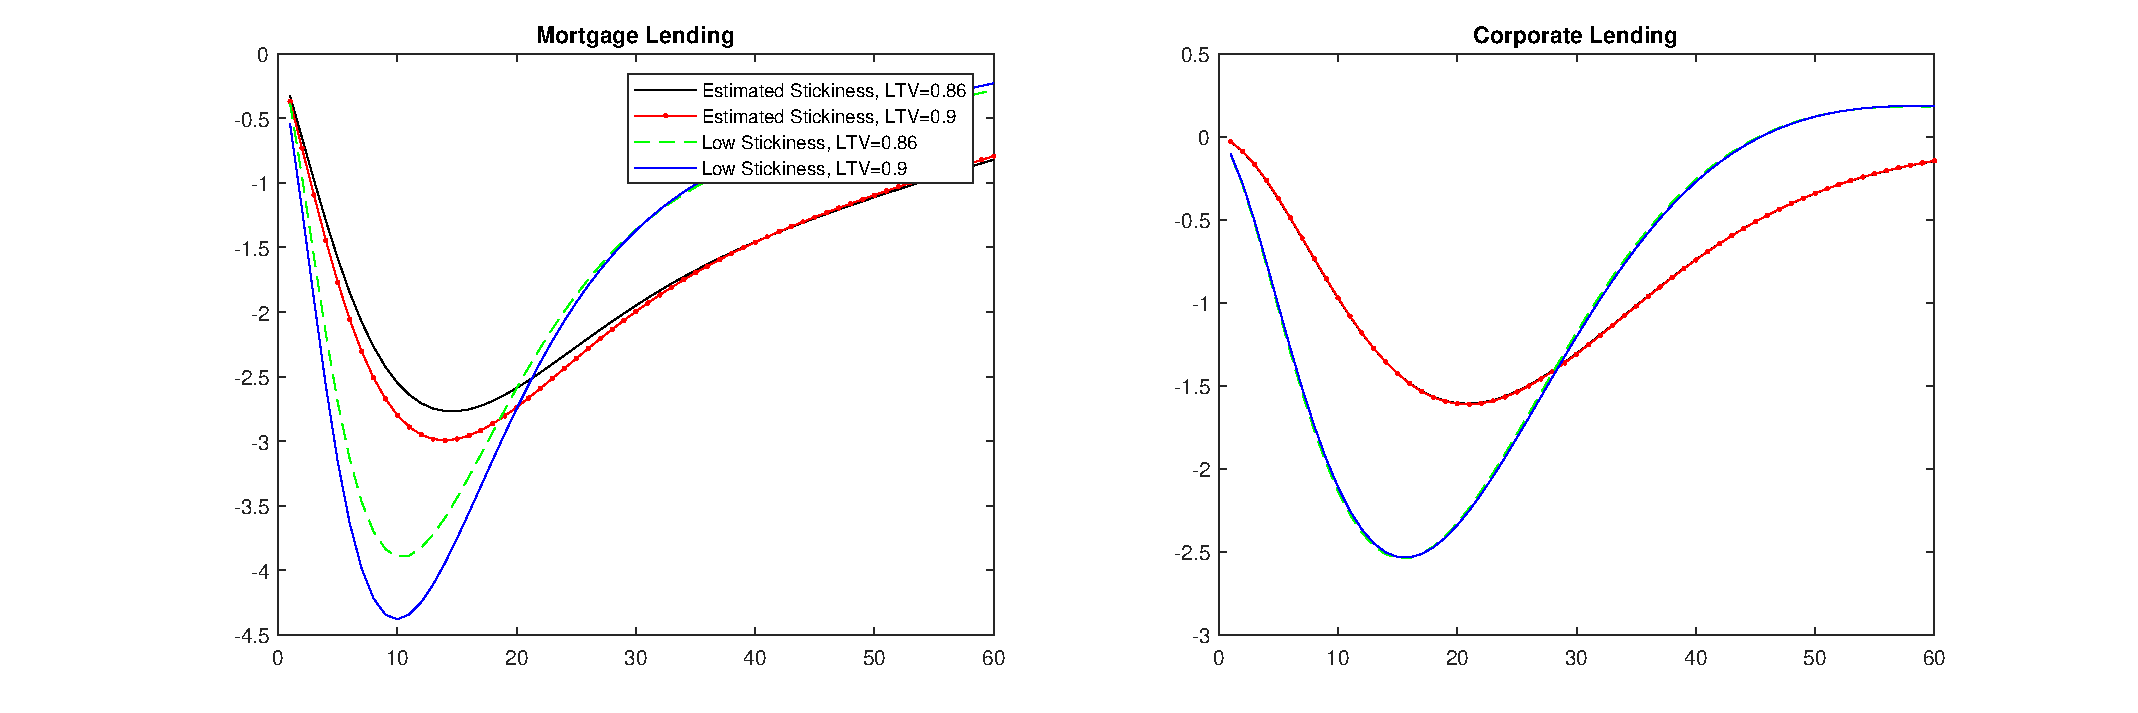
\includegraphics[scale=0.45]{stickiness_LTVECAB.pdf}}
\subfigure[Cumulative differences: 6.3 \% and 3.61 \%.]{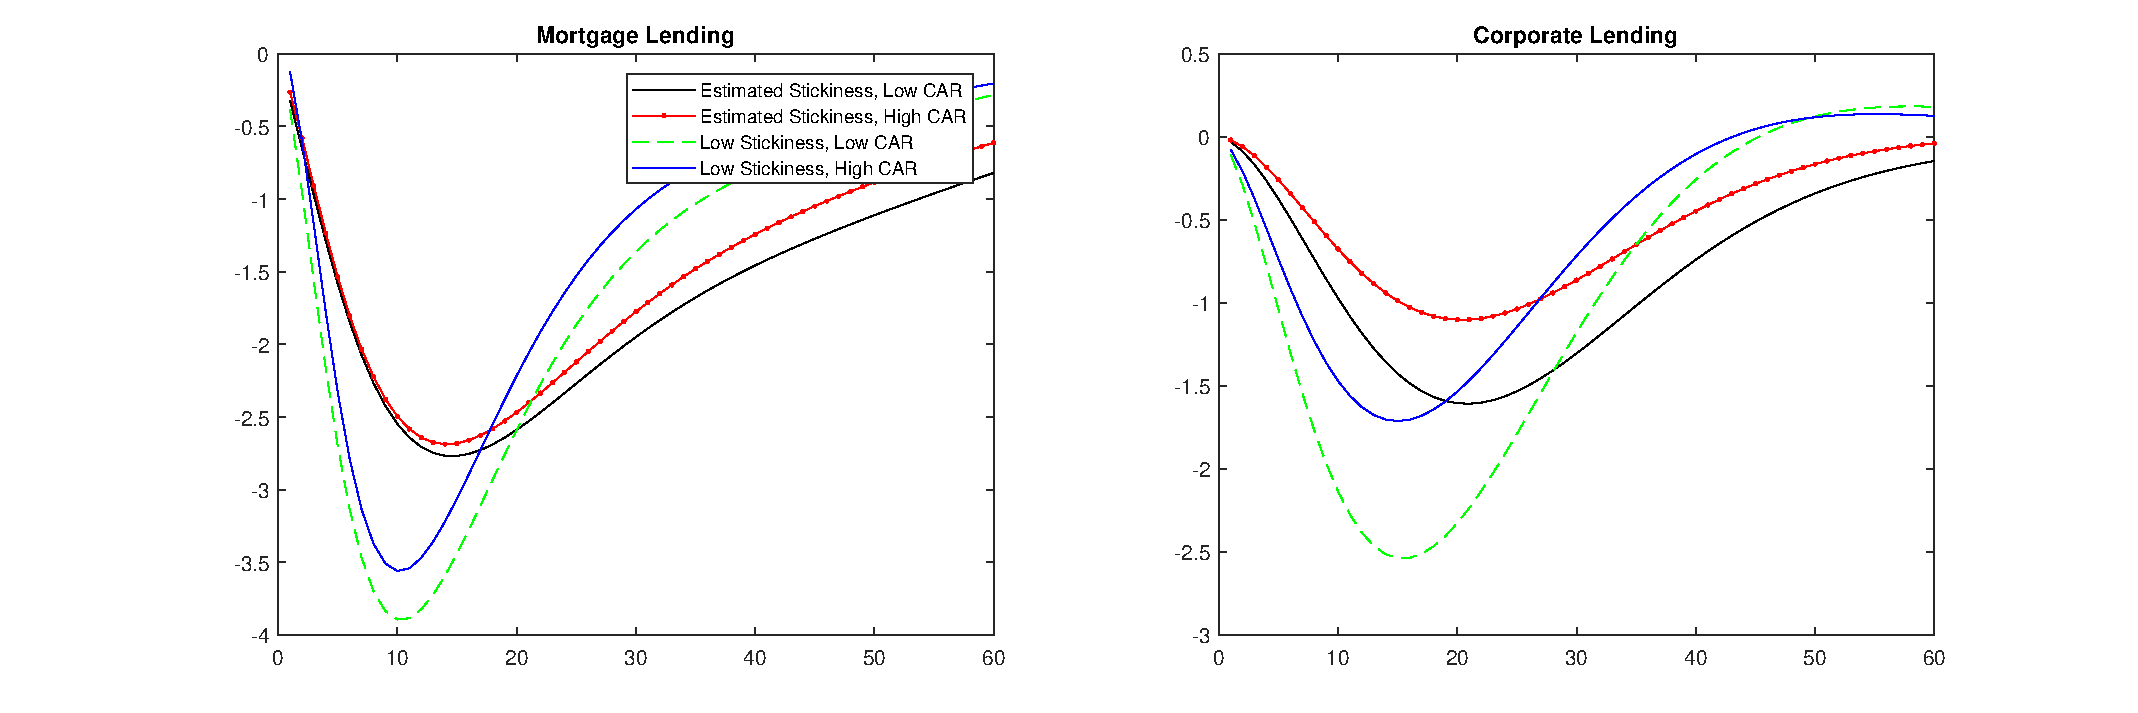
\includegraphics[scale=0.45]{stickiness_CARECAB.pdf}}
\end{figure}






\section*{Macroprudential Policy \& Steady State}

%\begin{figure}[H]
%\centering
%\caption{LTV limit with a baseline of 86 \%. welfare maximizing value is 89.4 \% if the weight on volatility is 0. It decreases to 86.6 \% if the weight on volatility is 0.1.
%\textbf{Welfare improvement: 0.014 \% and 0.0002 \% respectively.} } 
%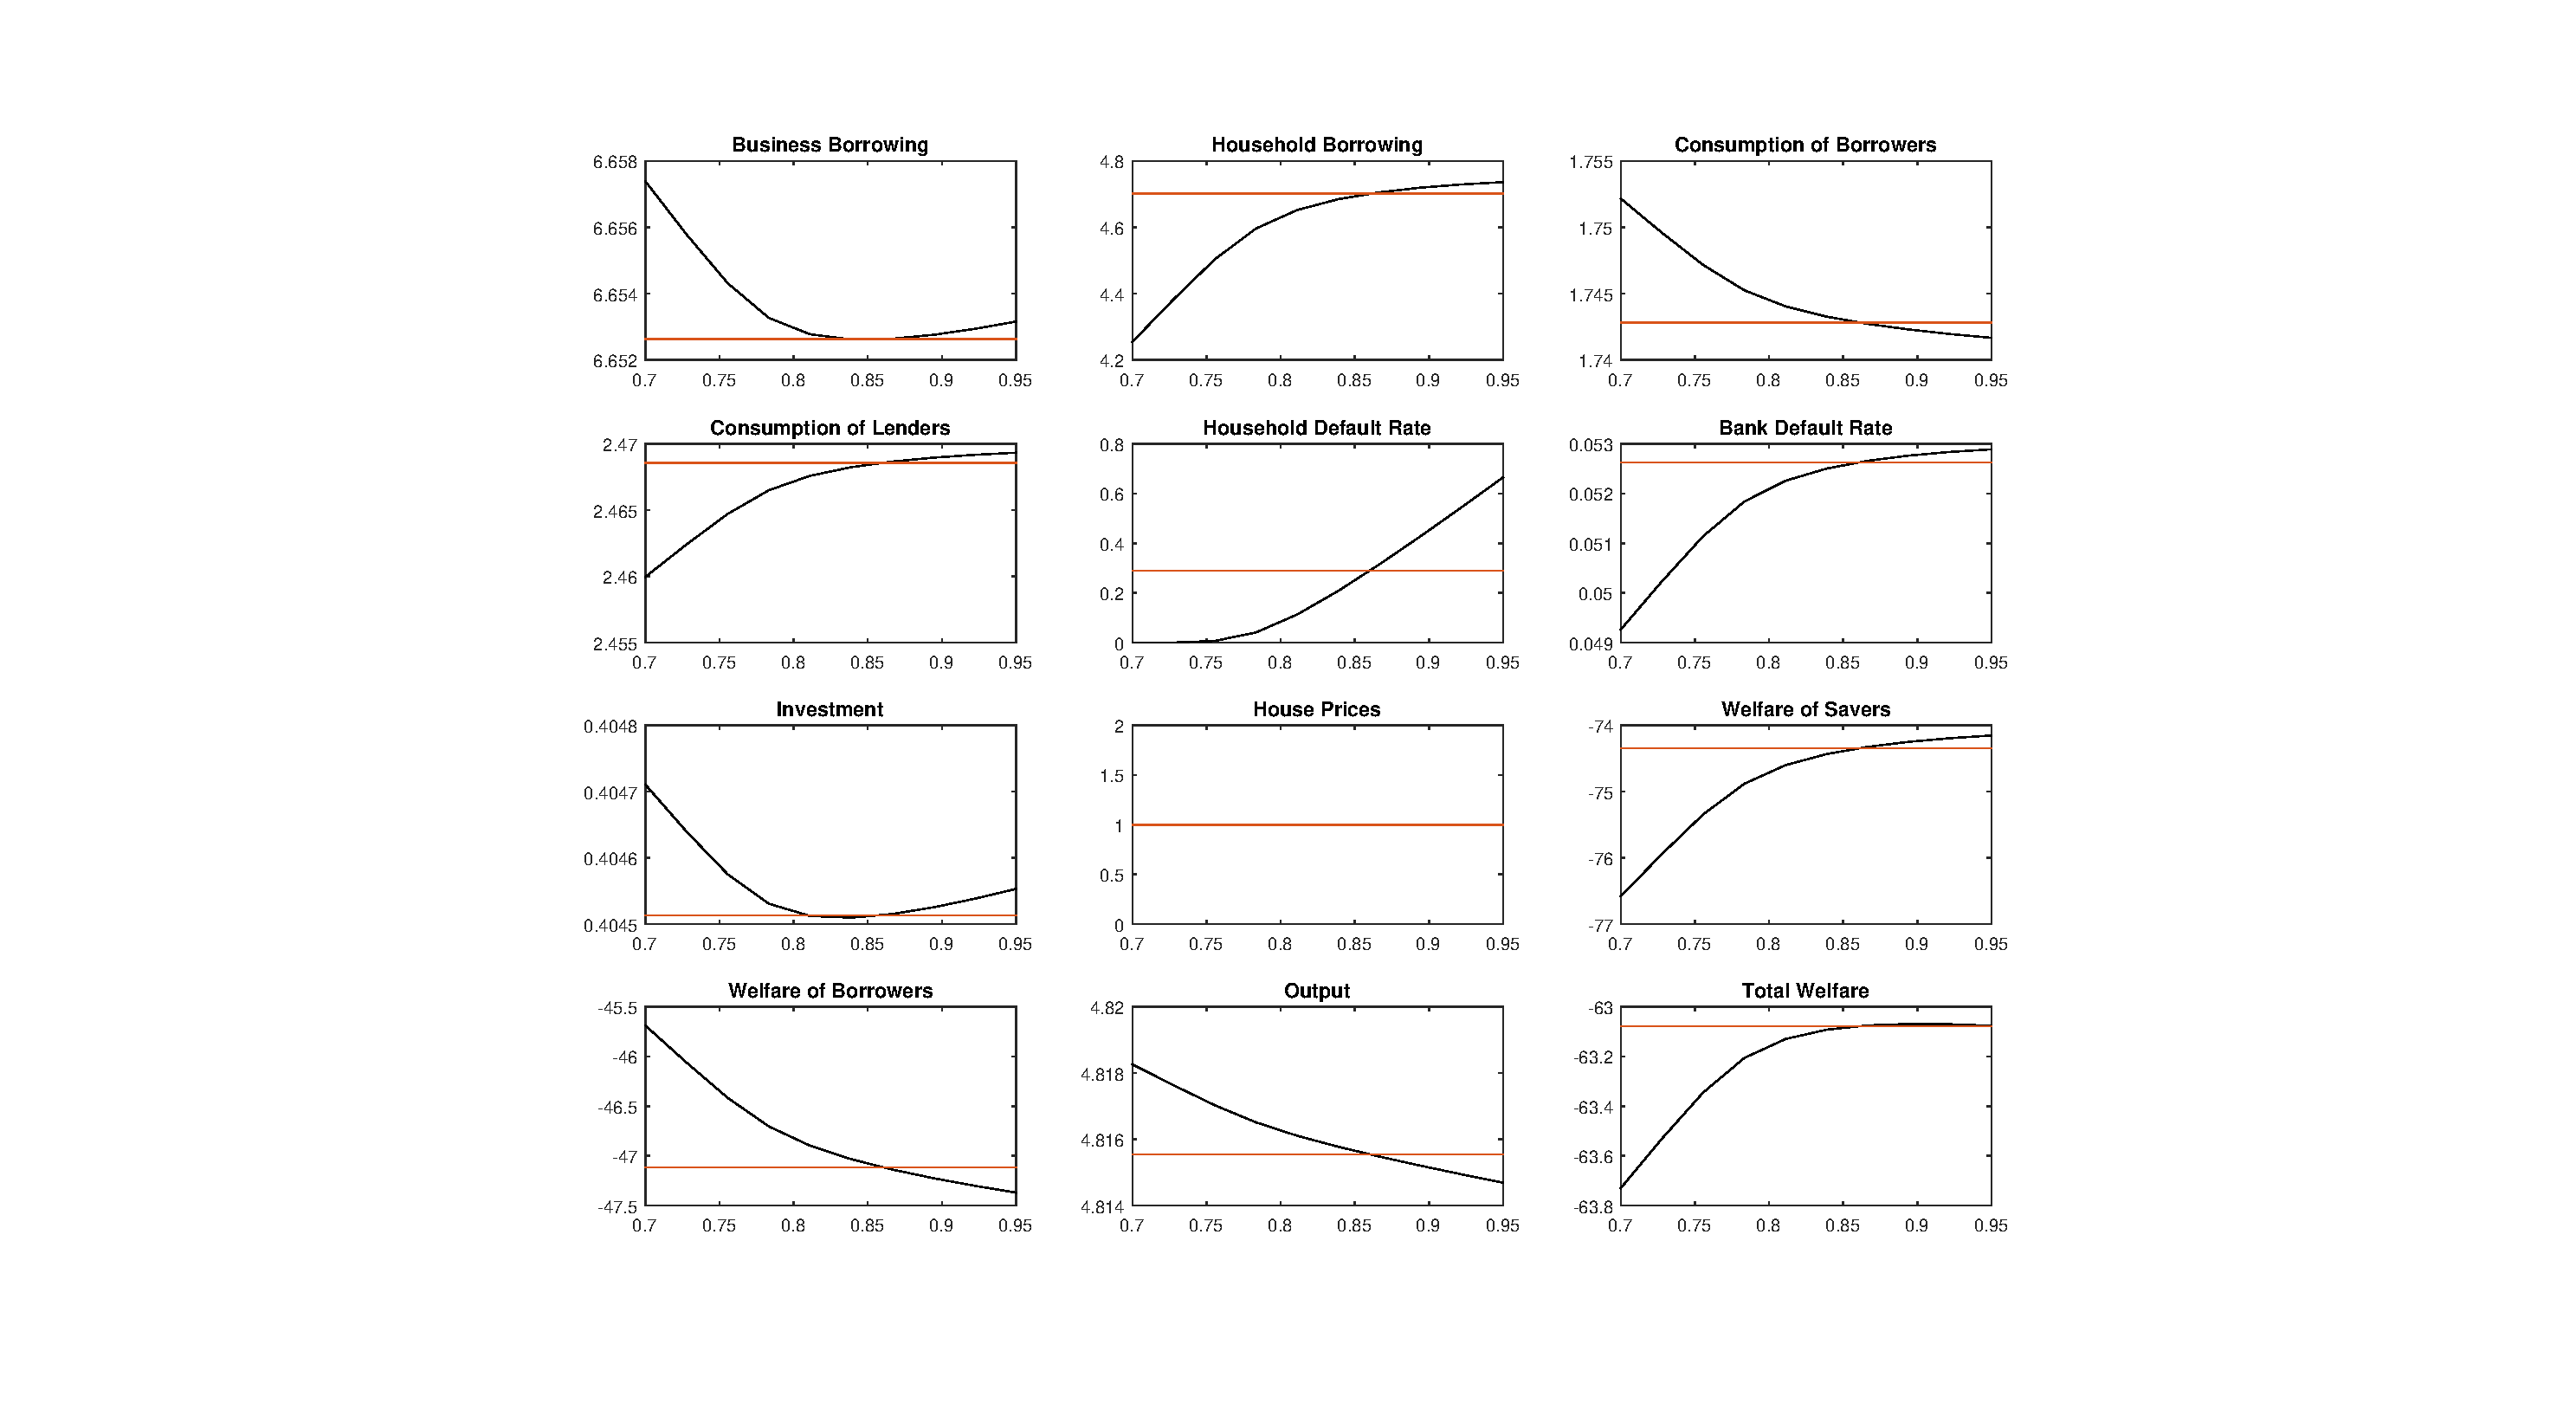
\includegraphics[scale=0.4]{WA1_level.pdf}\\
%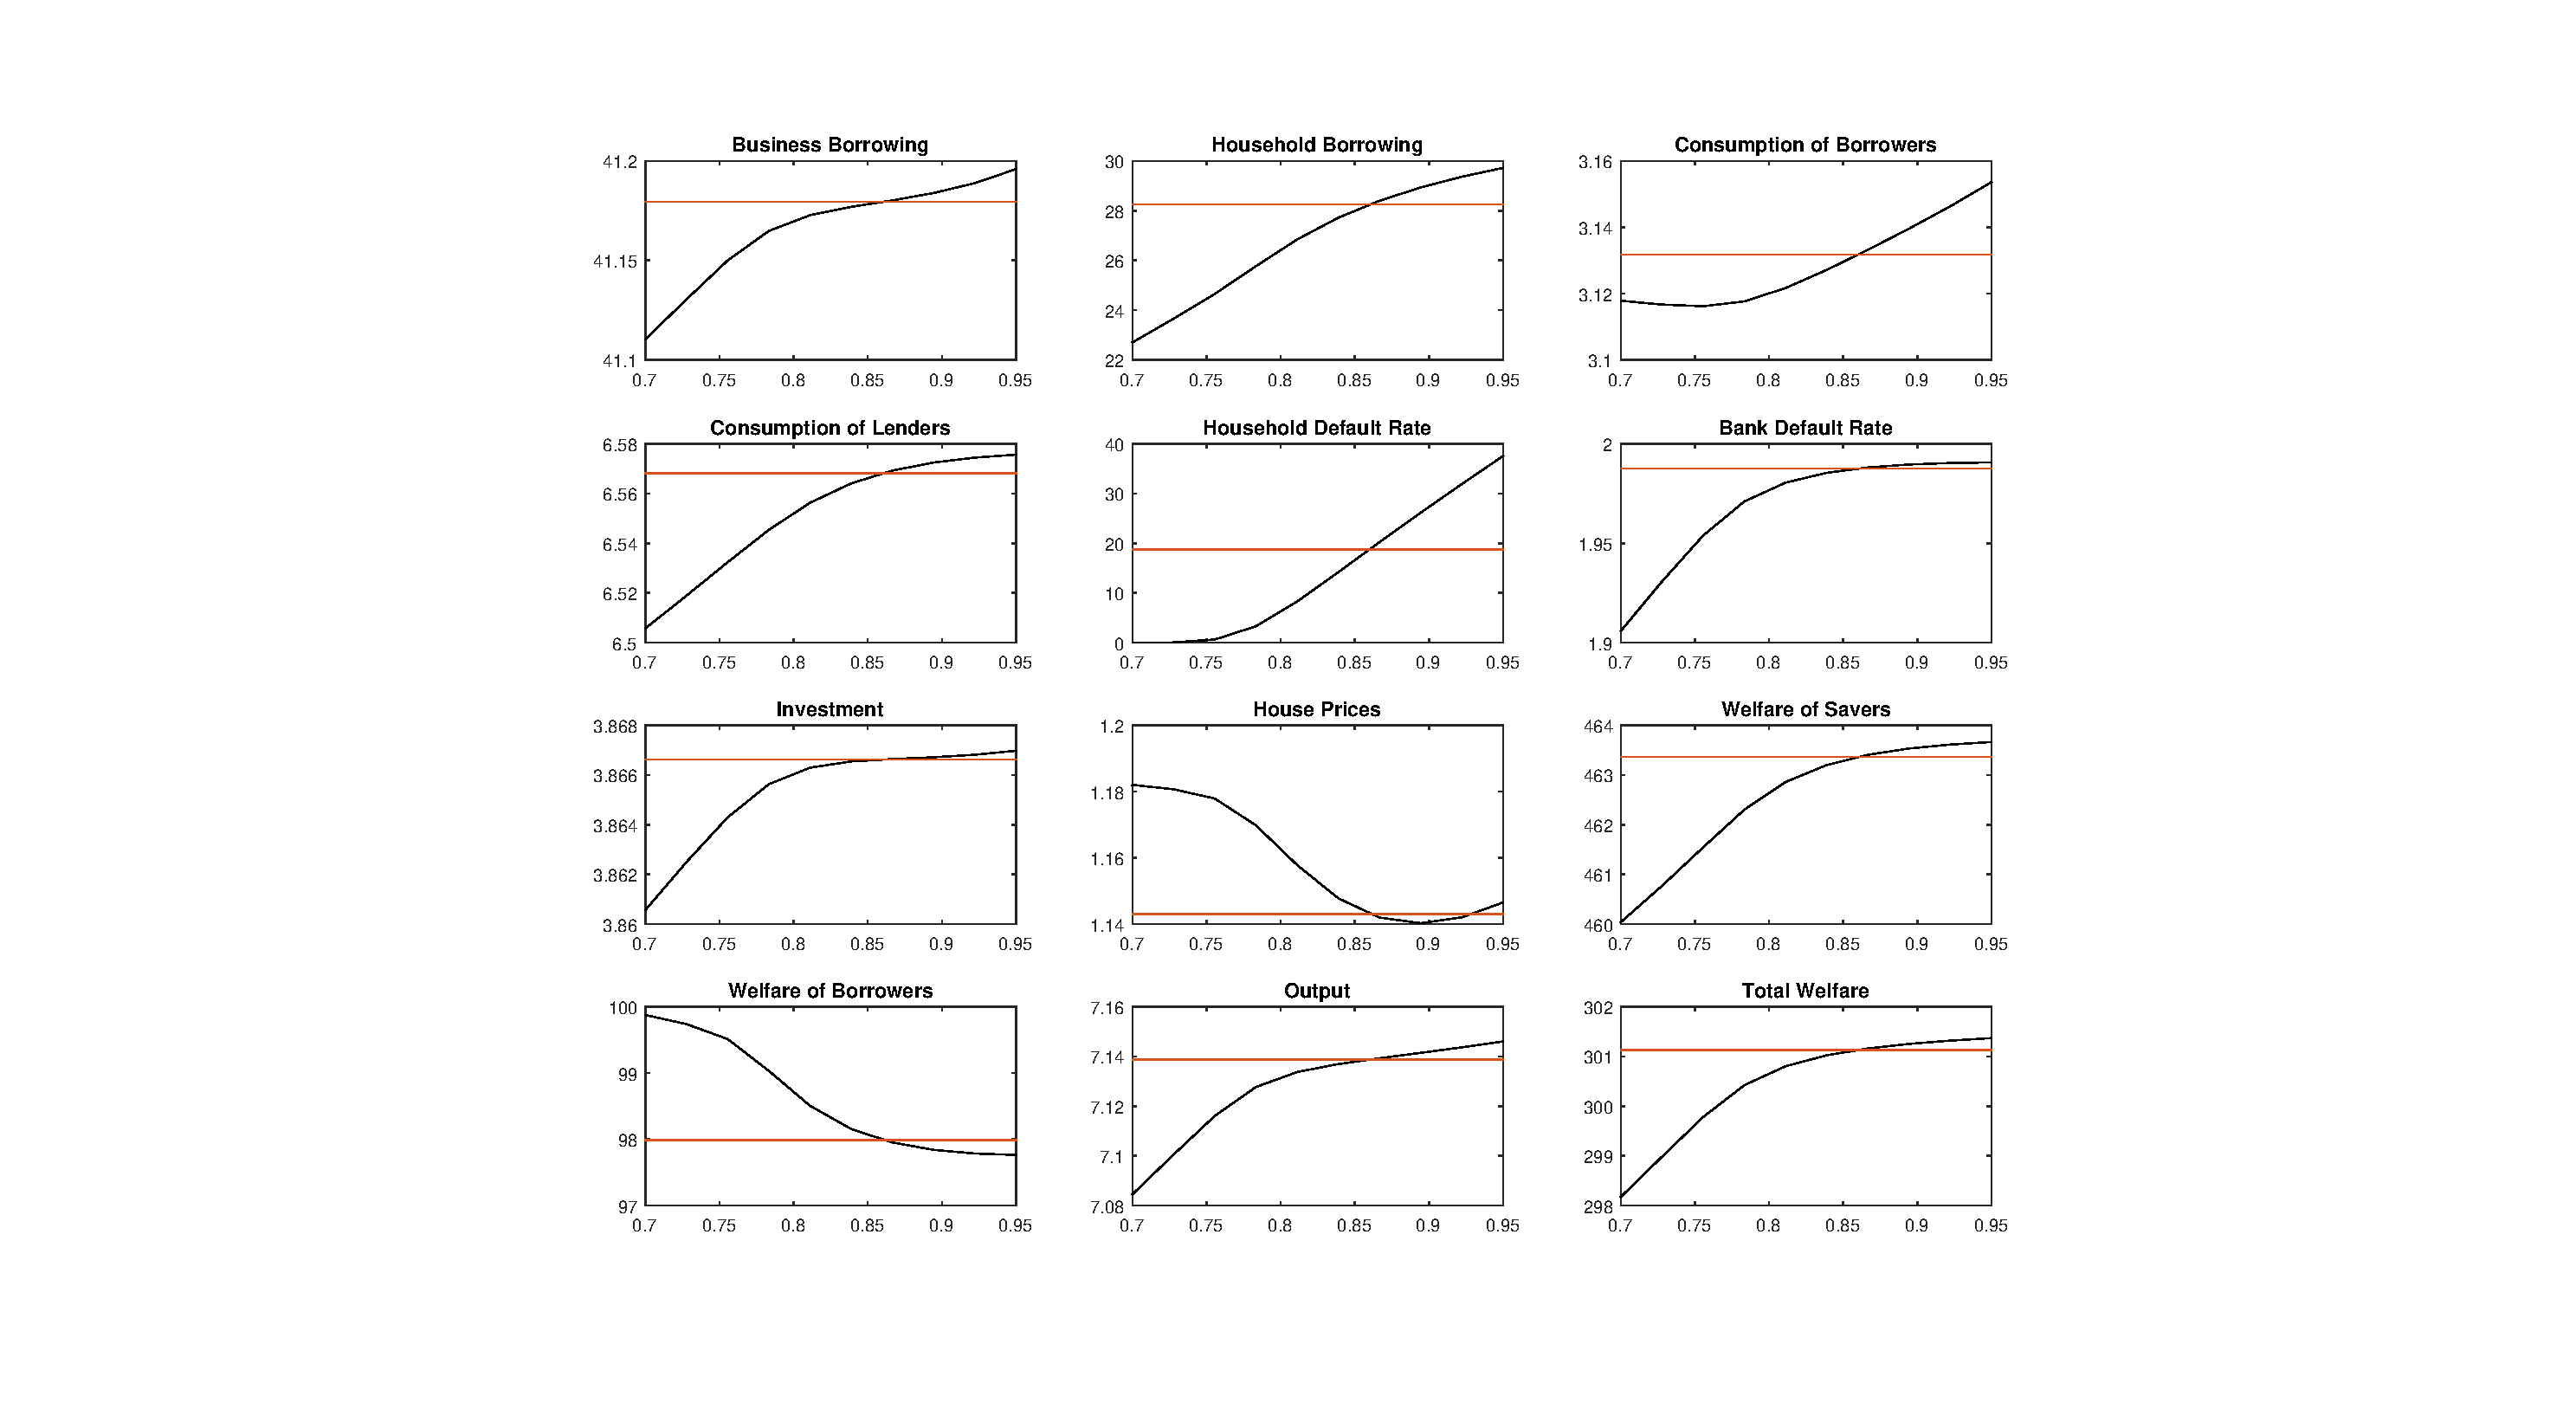
\includegraphics[scale=0.4]{WA1_var.pdf}
%\end{figure}



\begin{figure}[H]
\centering
\caption{Sectoral capital requirements on mortgage lending with a baseline of 11 \%. Welfare maximizing value is 20.7 \% with a weight of 0 on volatility. It decreases to 17.6 \% with a weight of 0.1 on the volatility.
\label{steadystate_SCR_figure}
\textbf{Welfare improvement: 7.47 \% and 4.26 \% respectively.} } 
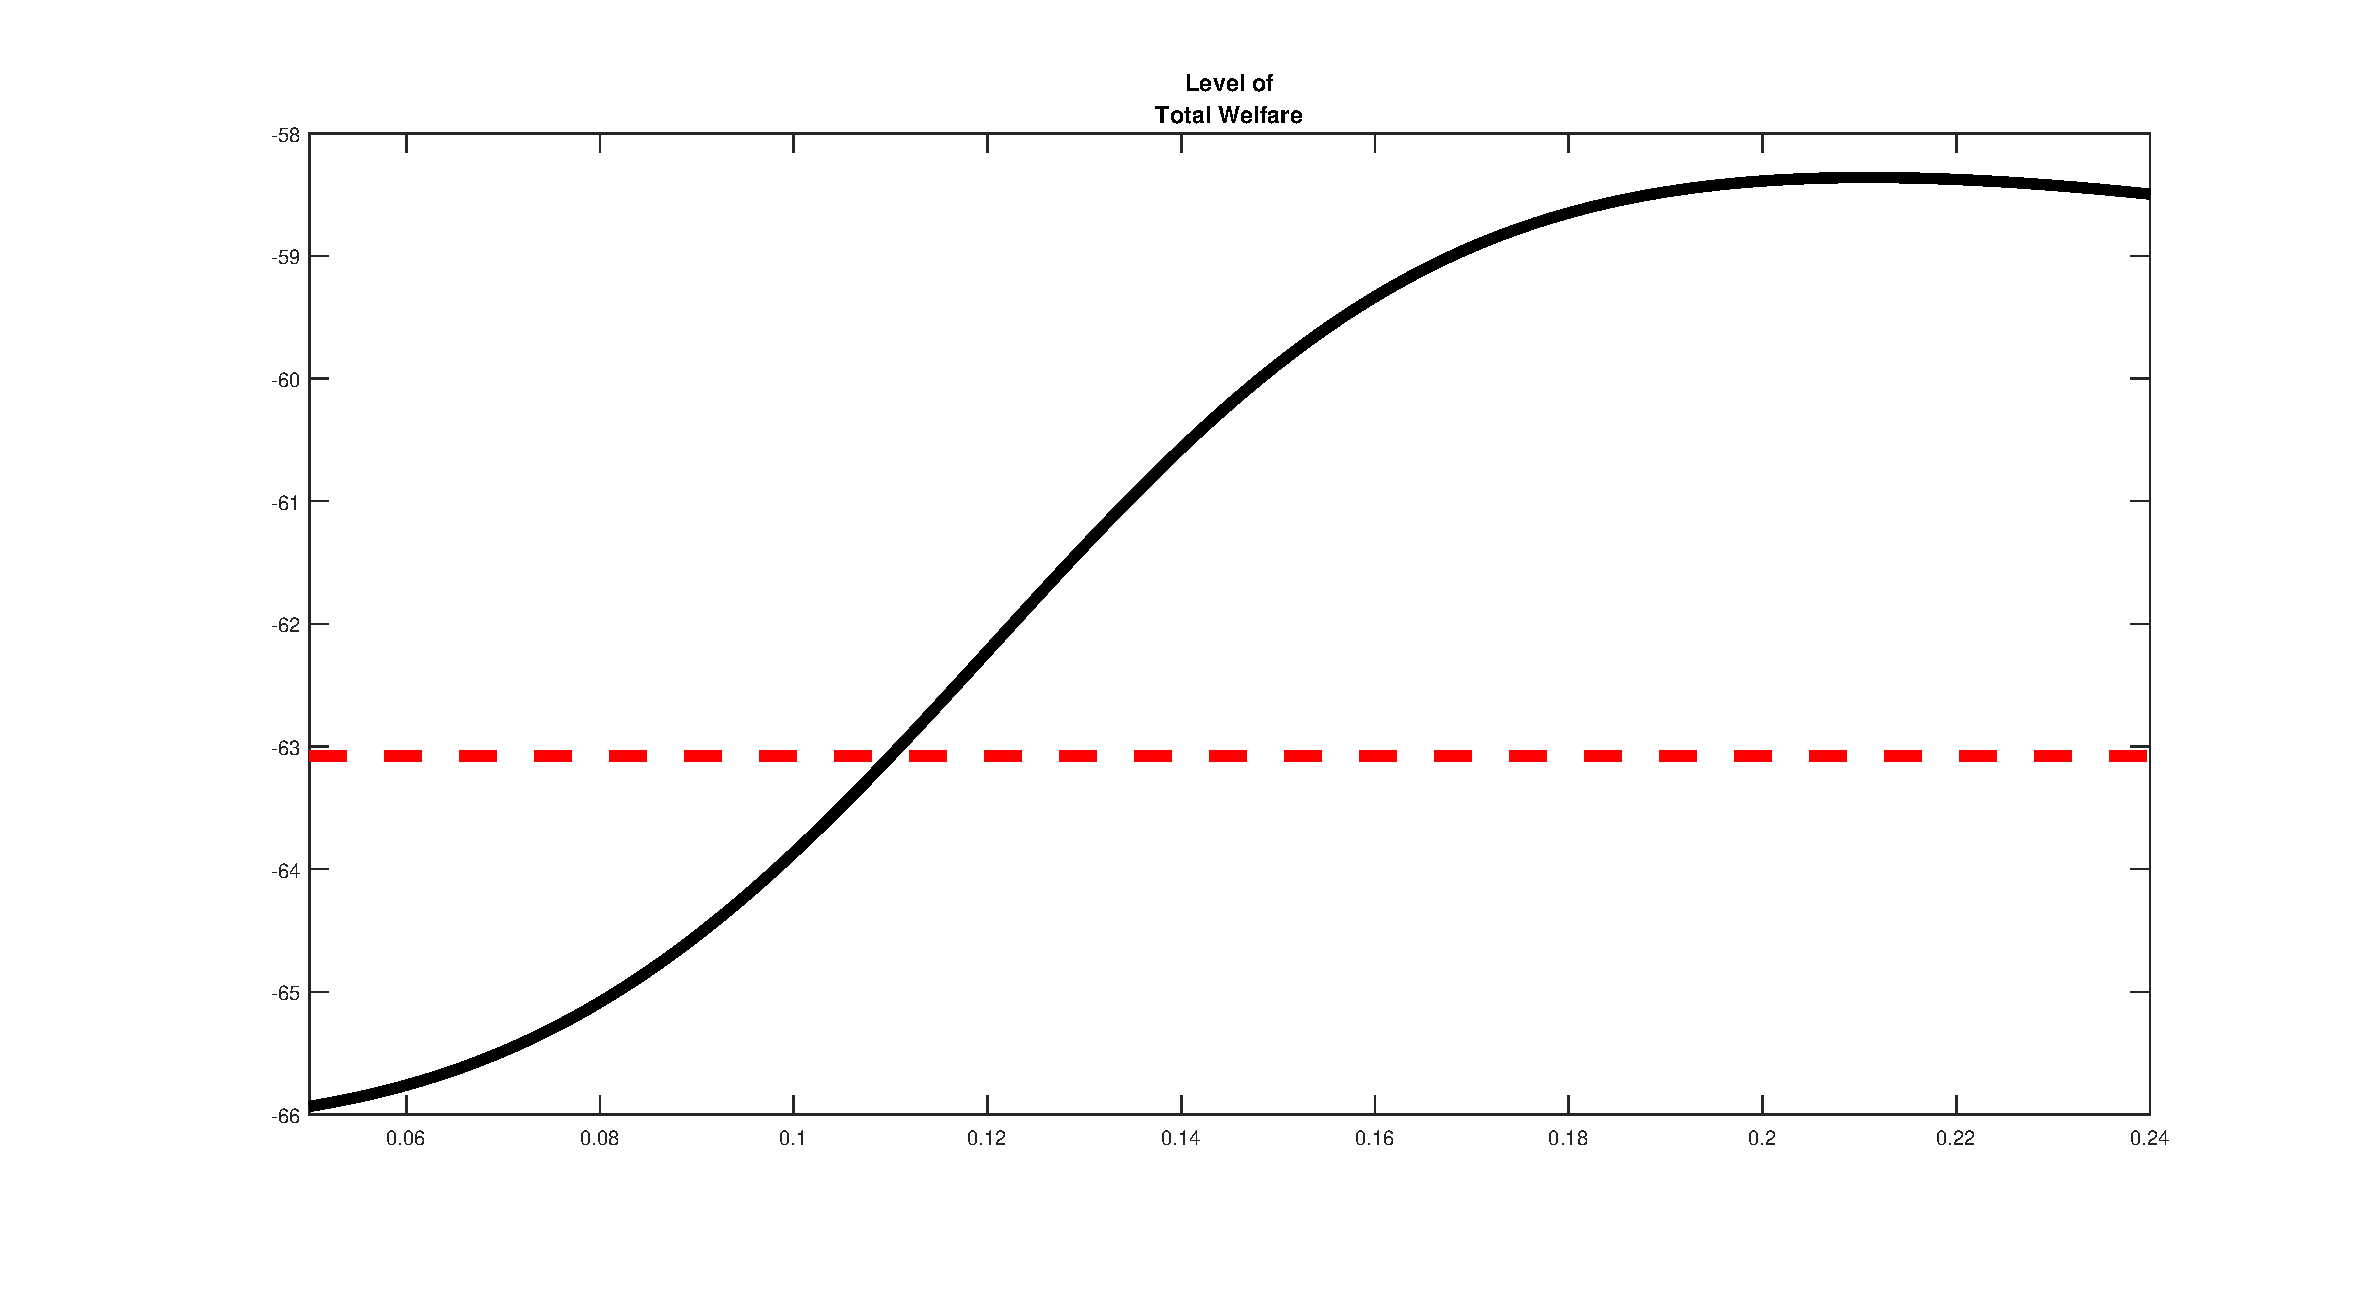
\includegraphics[scale=0.2]{welfare_SCR_housing_level.pdf}
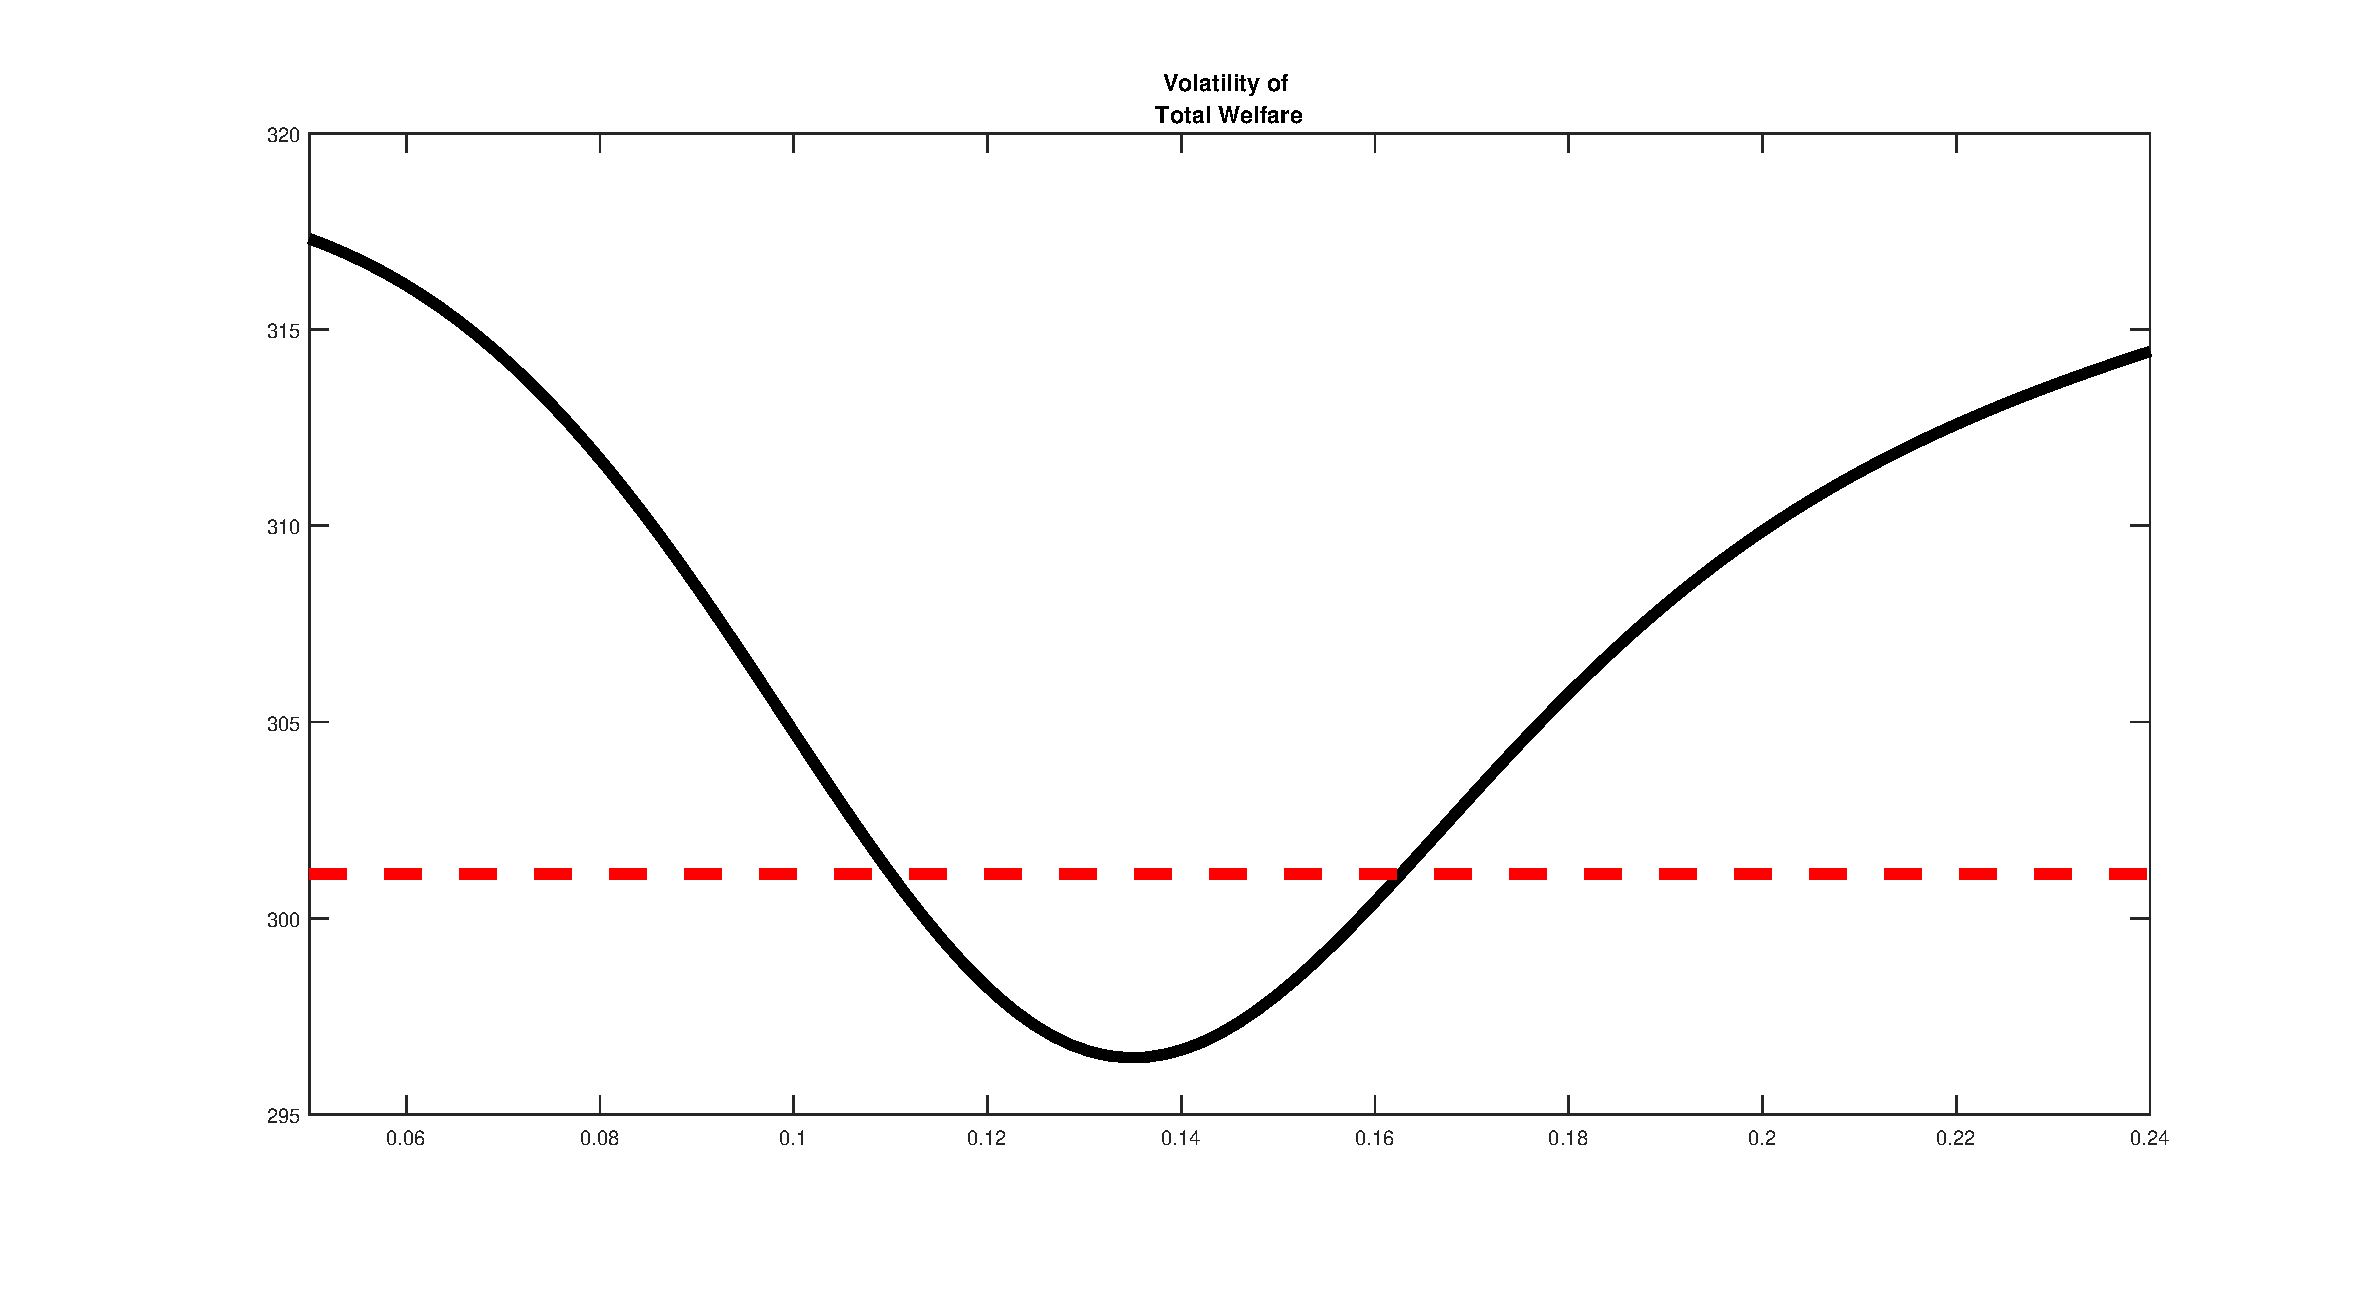
\includegraphics[scale=0.2]{welfare_SCR_housing_var.pdf}\\
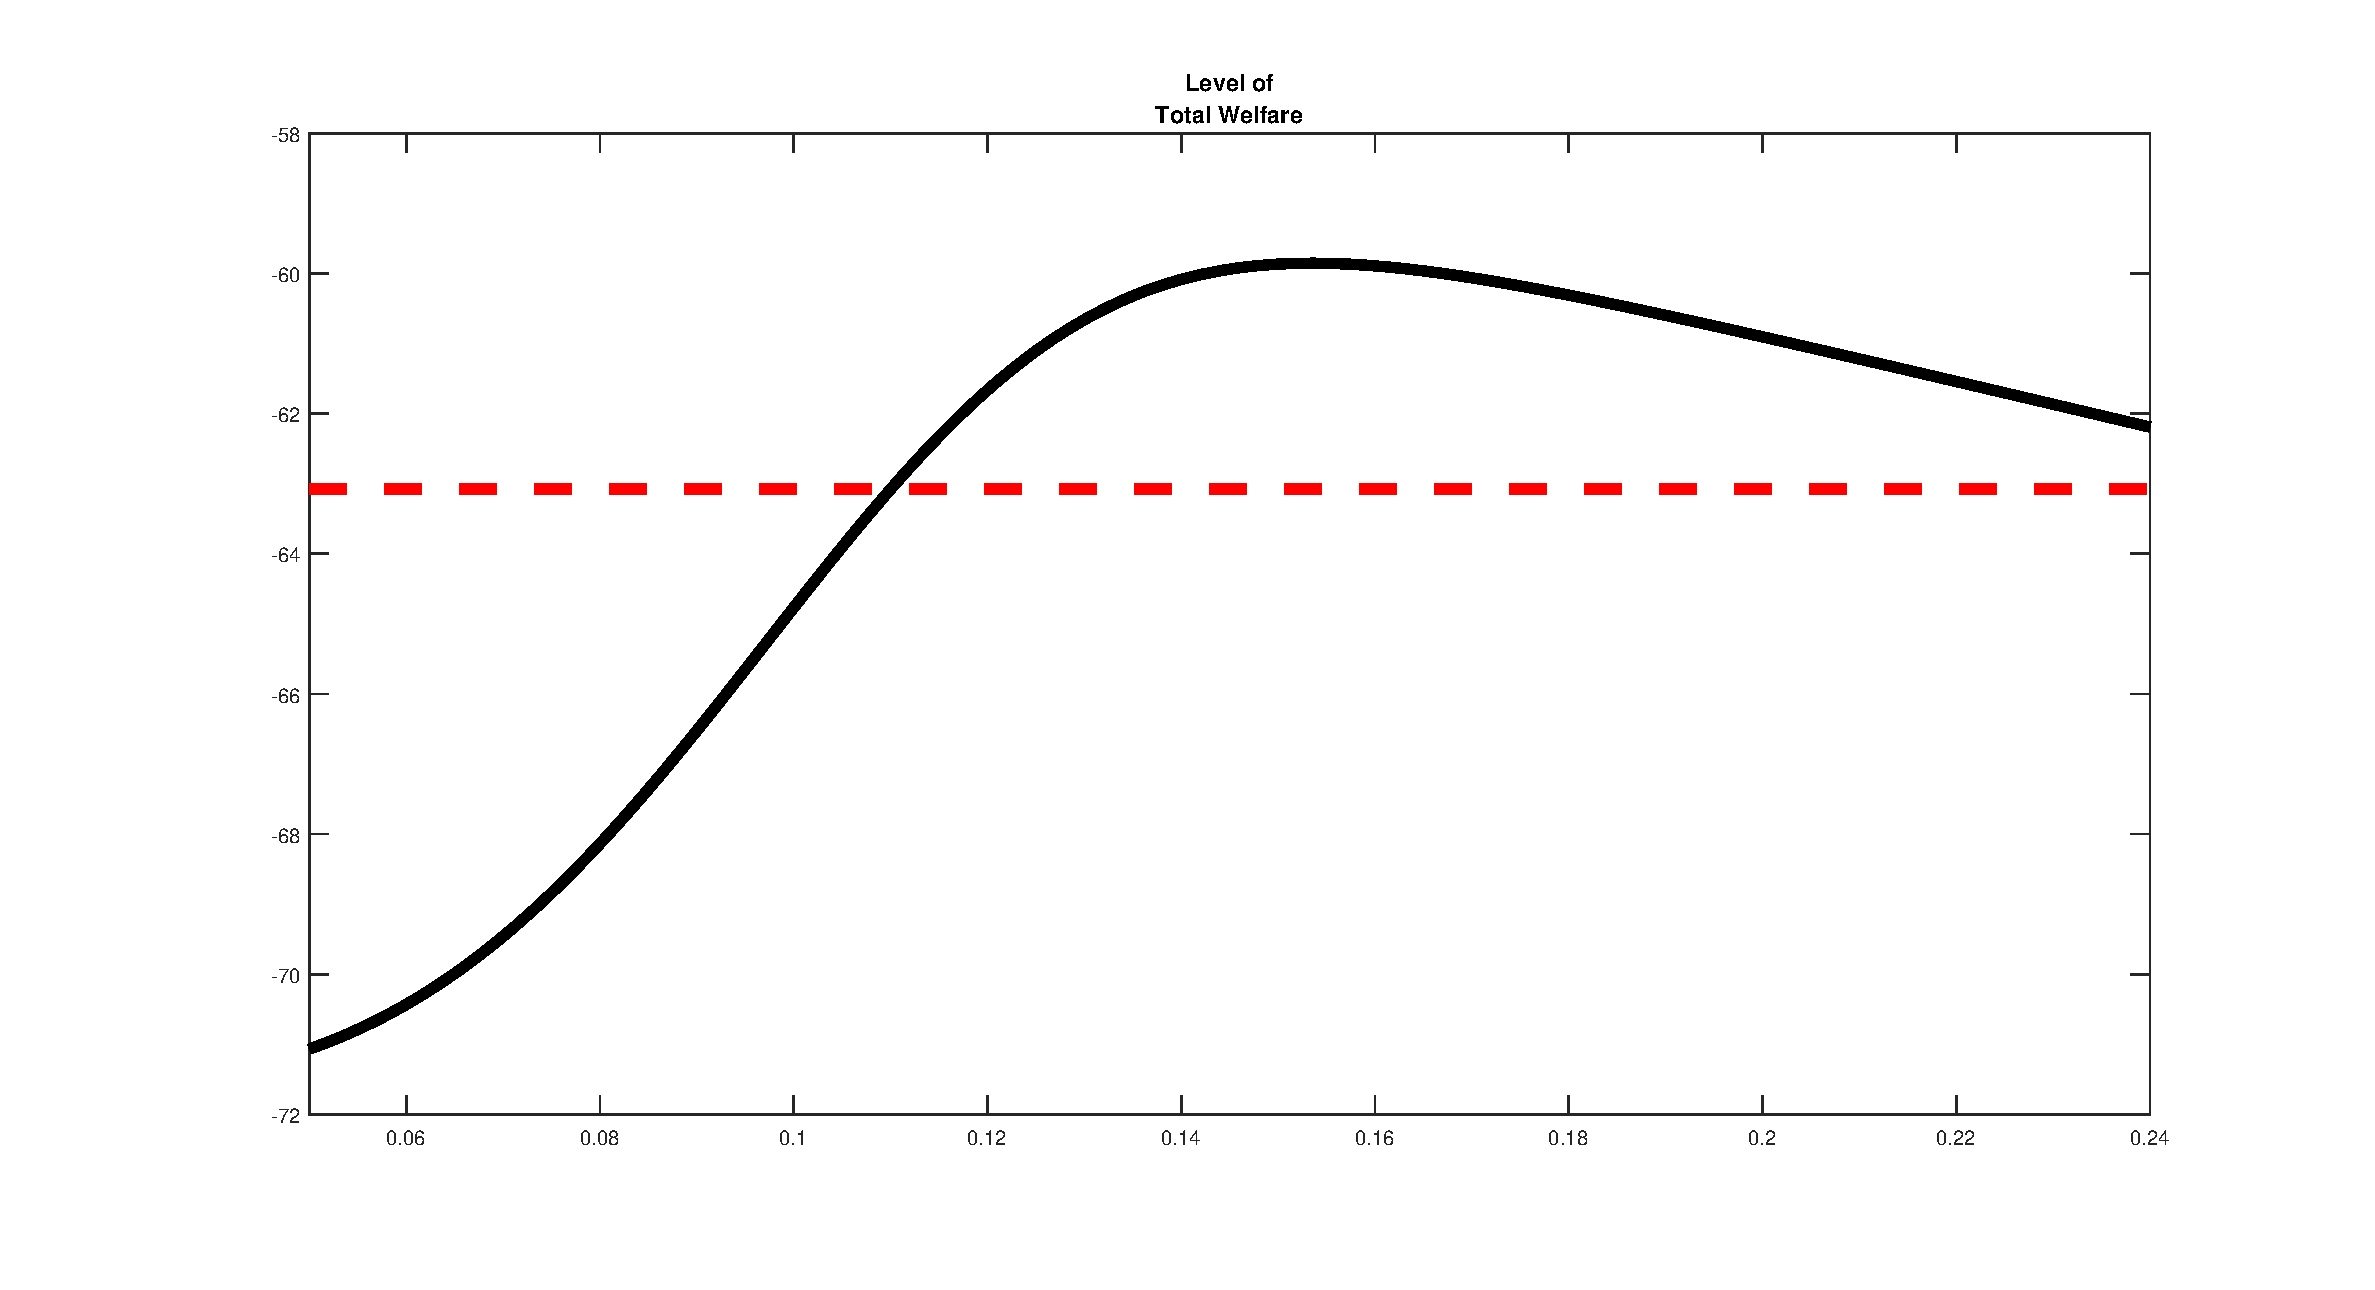
\includegraphics[scale=0.2]{welfare_CAR_level.pdf}
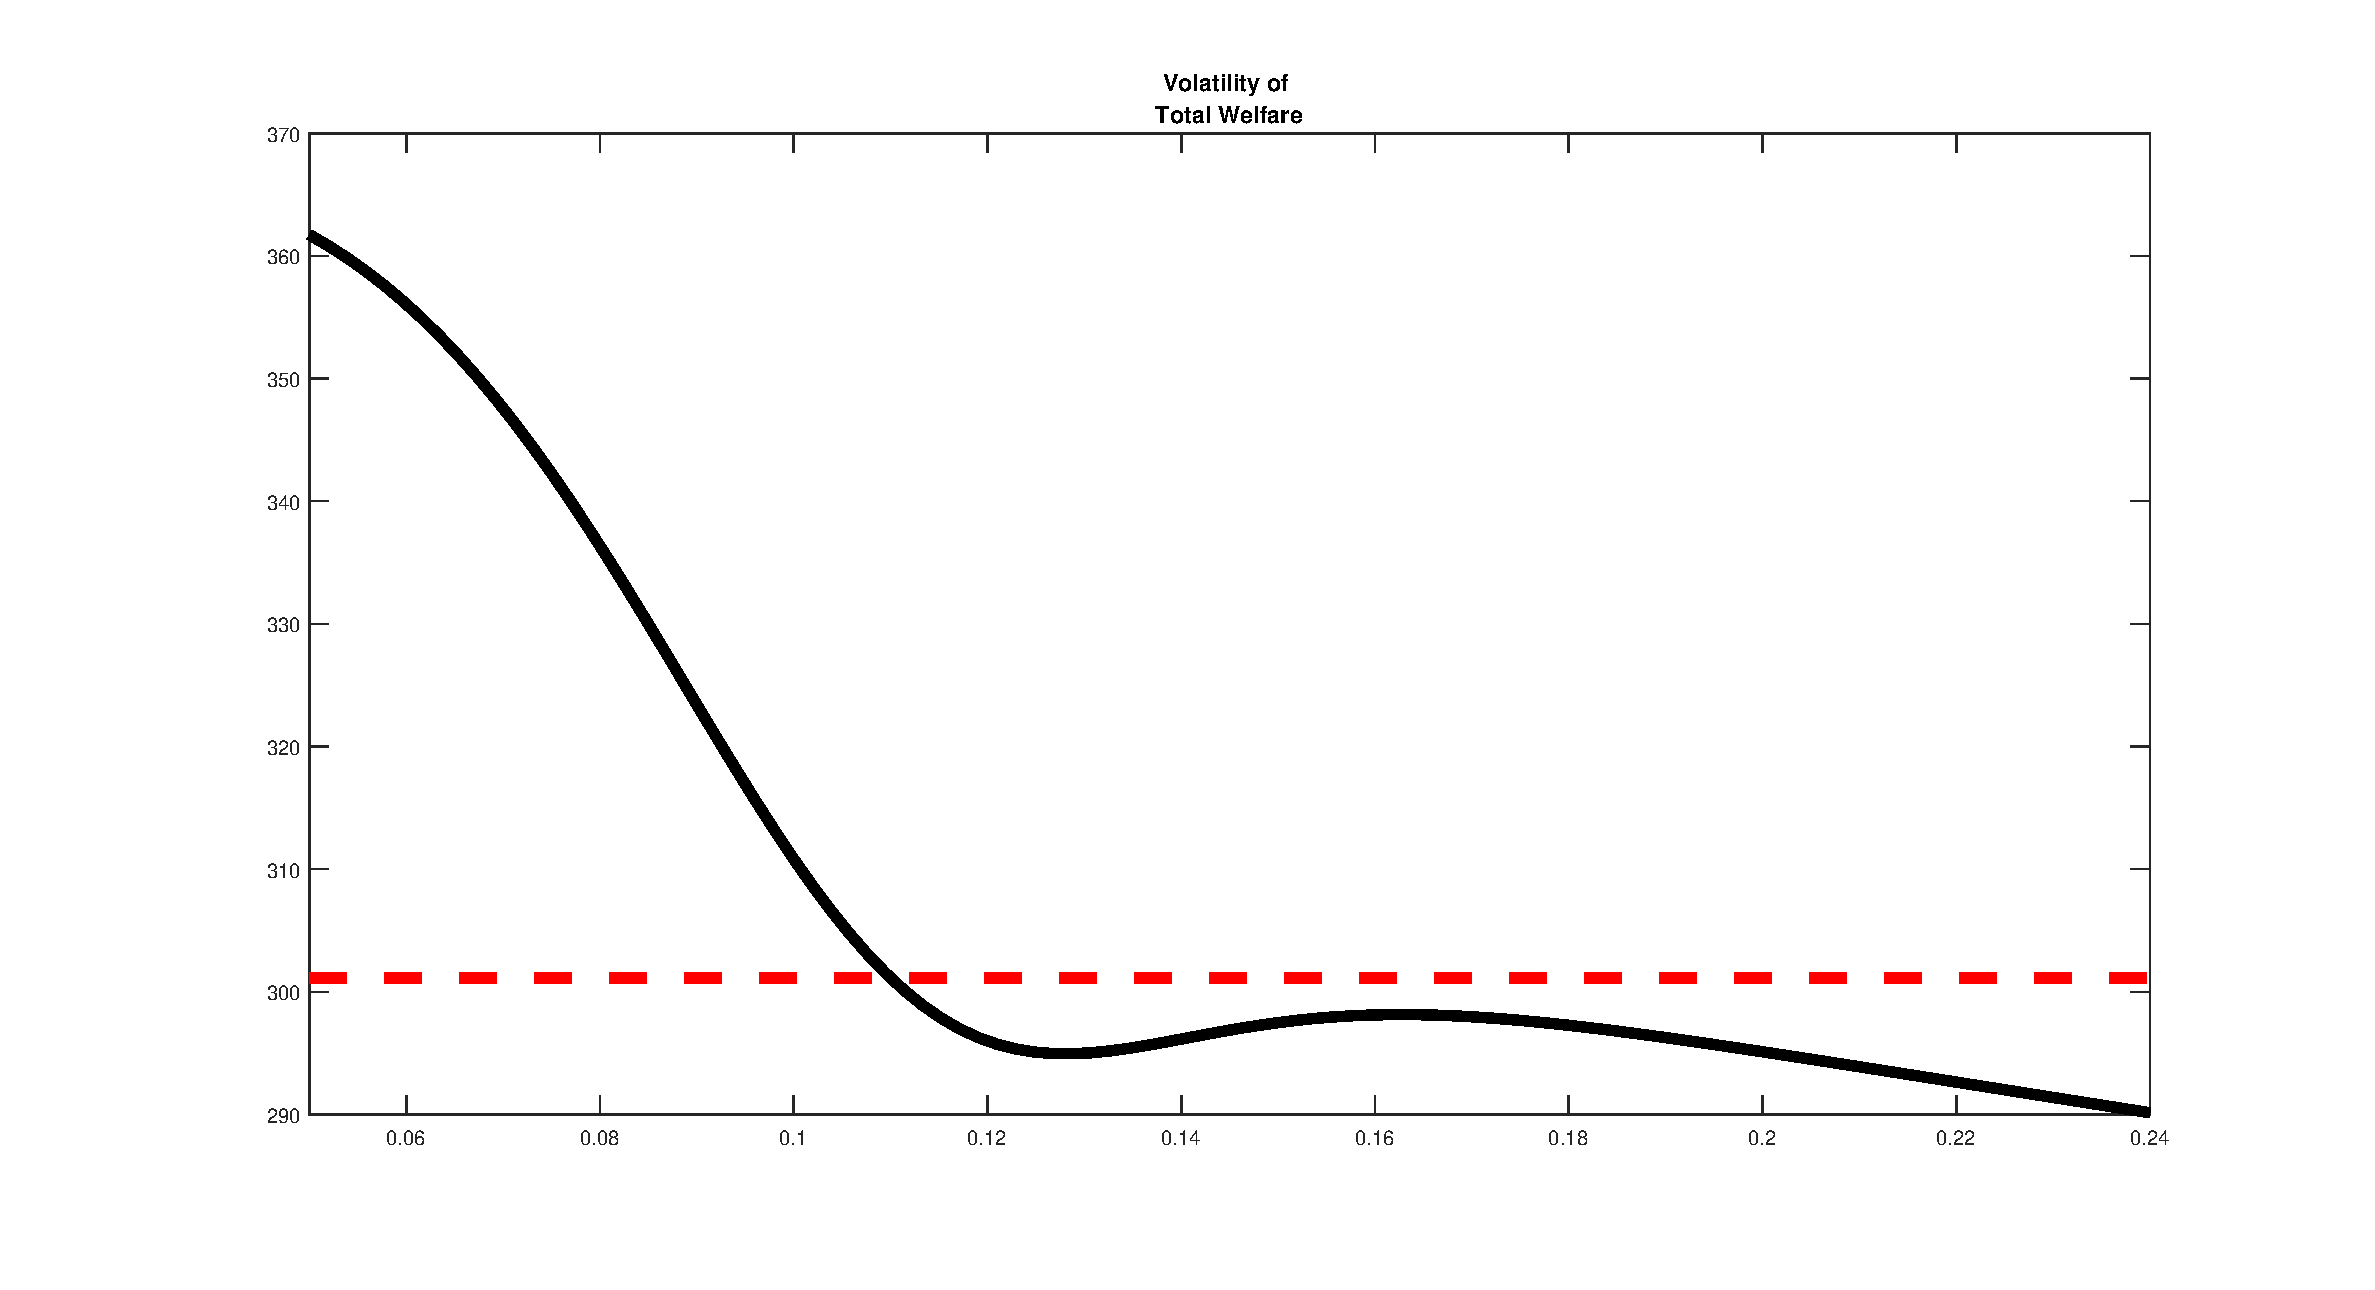
\includegraphics[scale=0.2]{welfare_CAR_var.pdf}
\end{figure}


%\begin{figure}[H]
%\centering
%\caption{Sectoral capital requirements on corporate lending with a baseline of 11 \%/ Welfare maximizing value is 15.5 with a weight of 0 on volatility. It increases to 16.7 \% with a weight of 0.1 on volatility. 
%\textbf{Welfare improvement: 3.33 \% and 3.22 \% respectively. } } 
%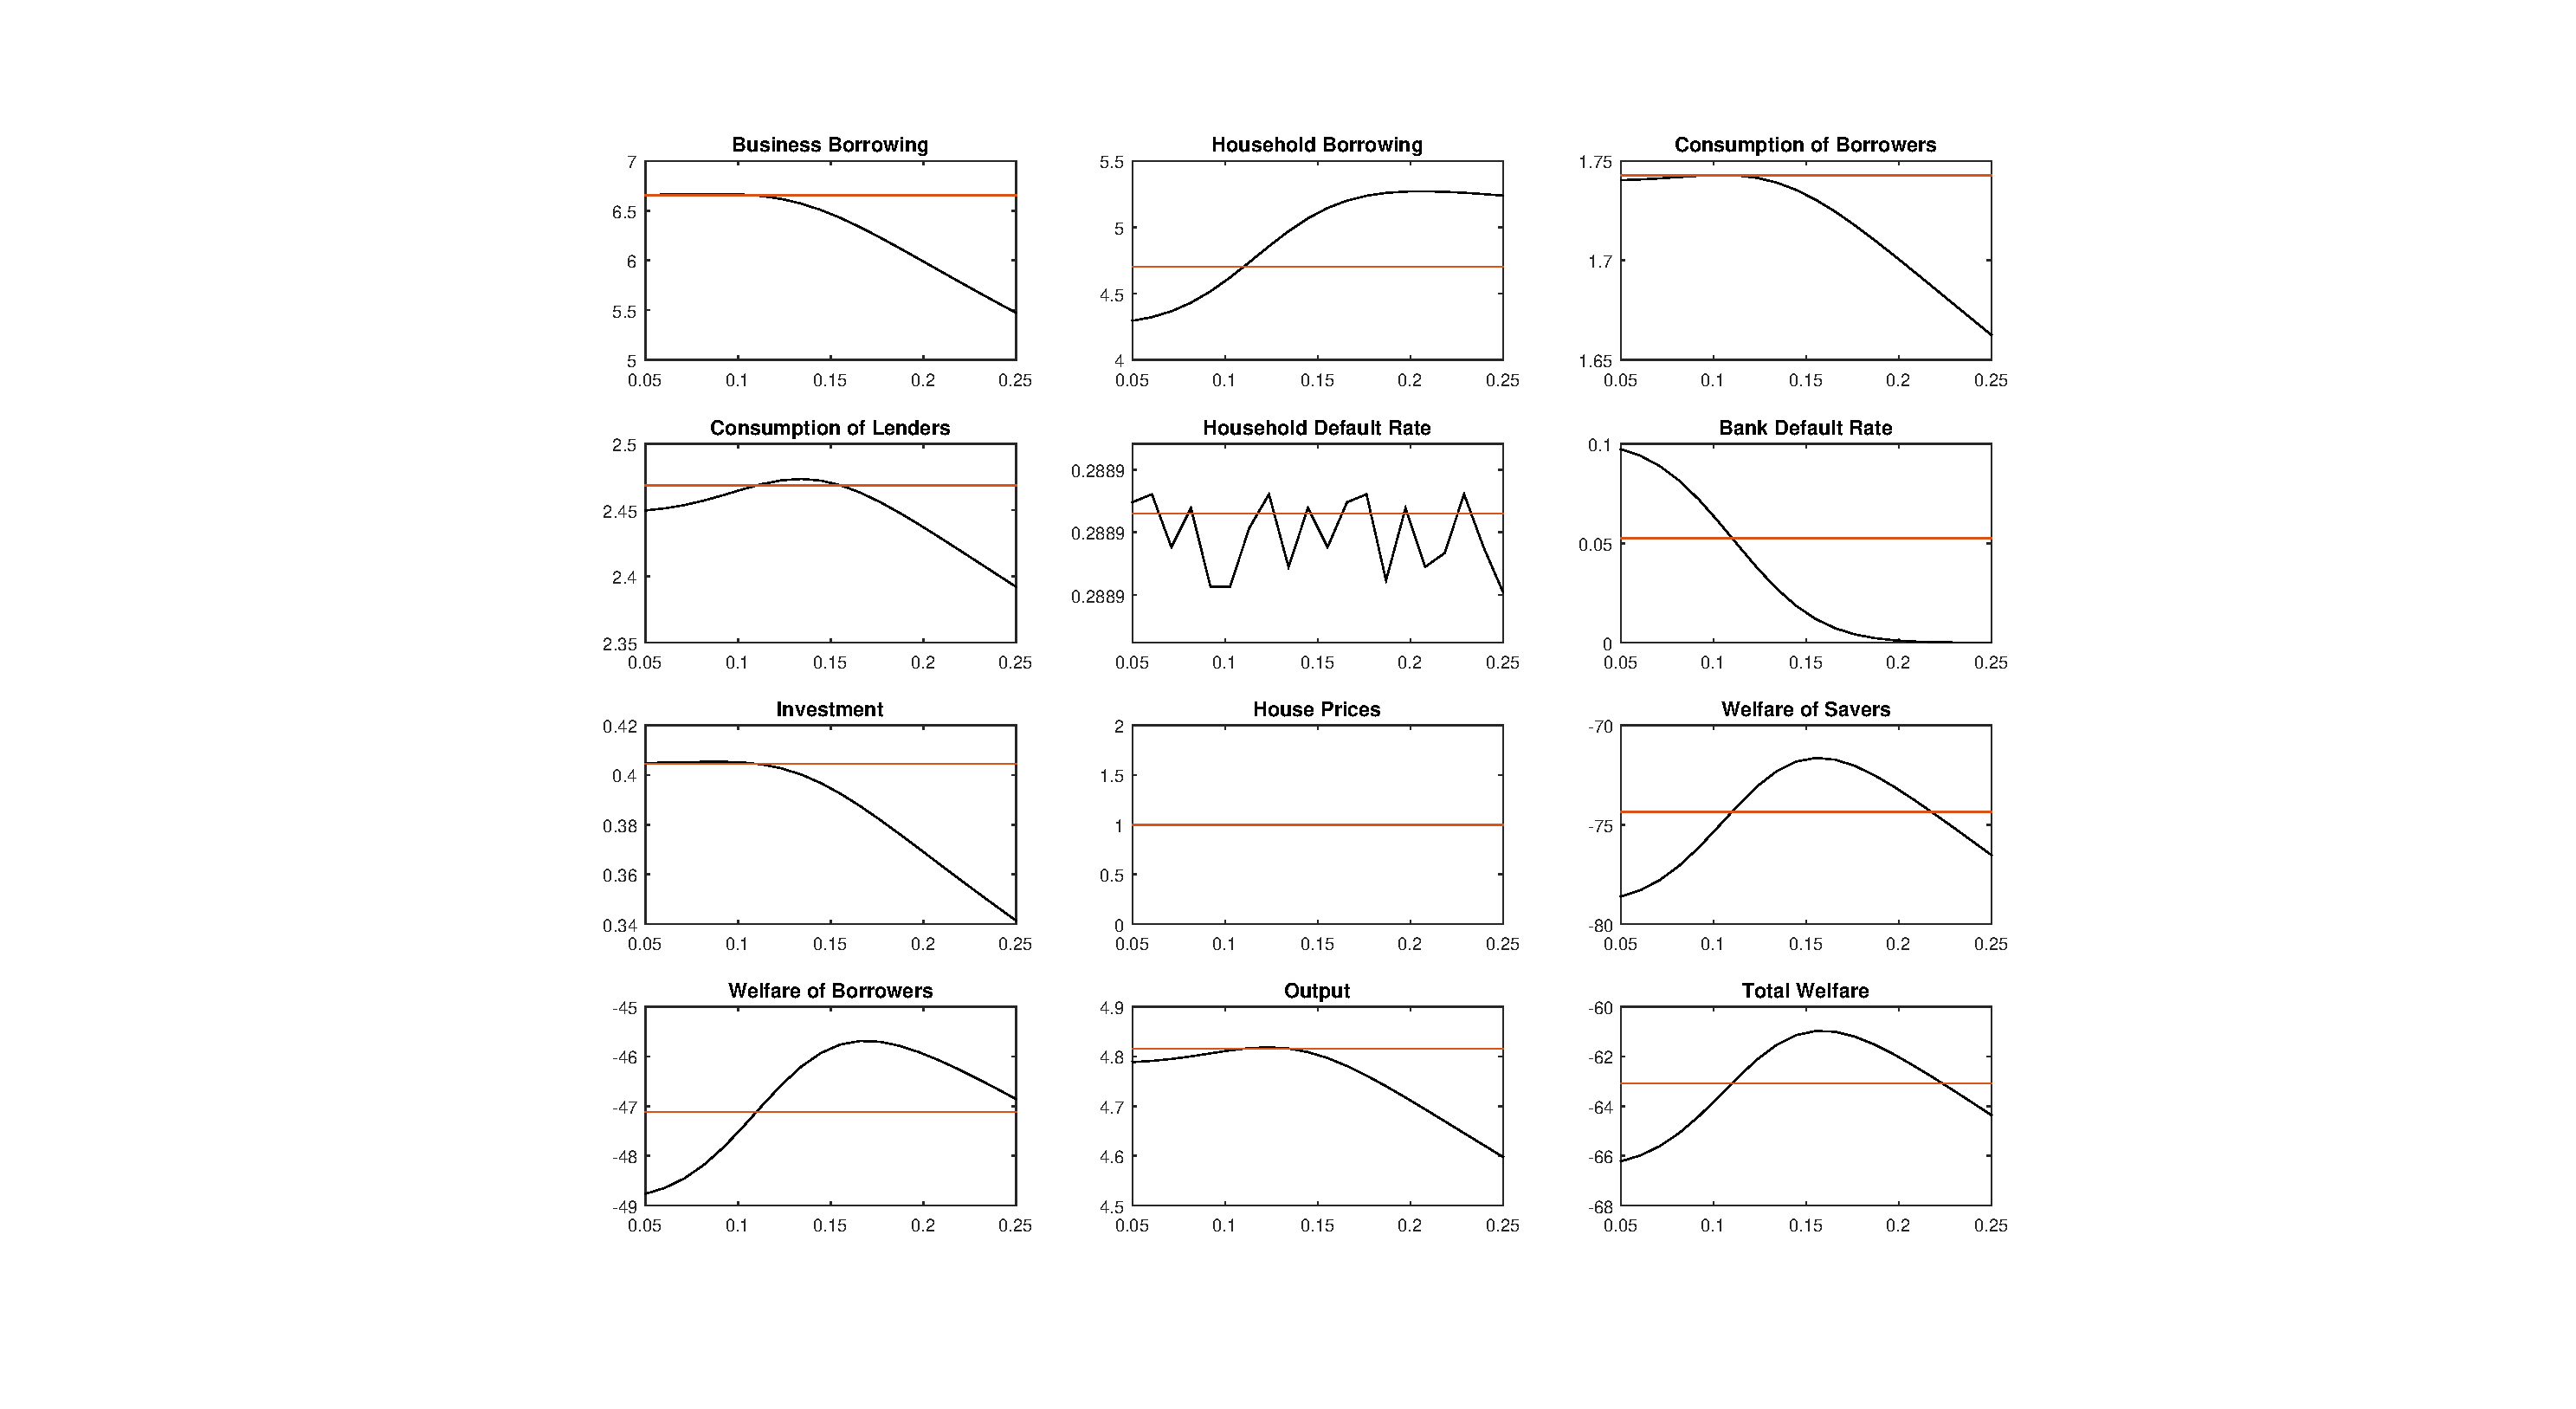
\includegraphics[scale=0.4]{WA3_level.pdf}\\
%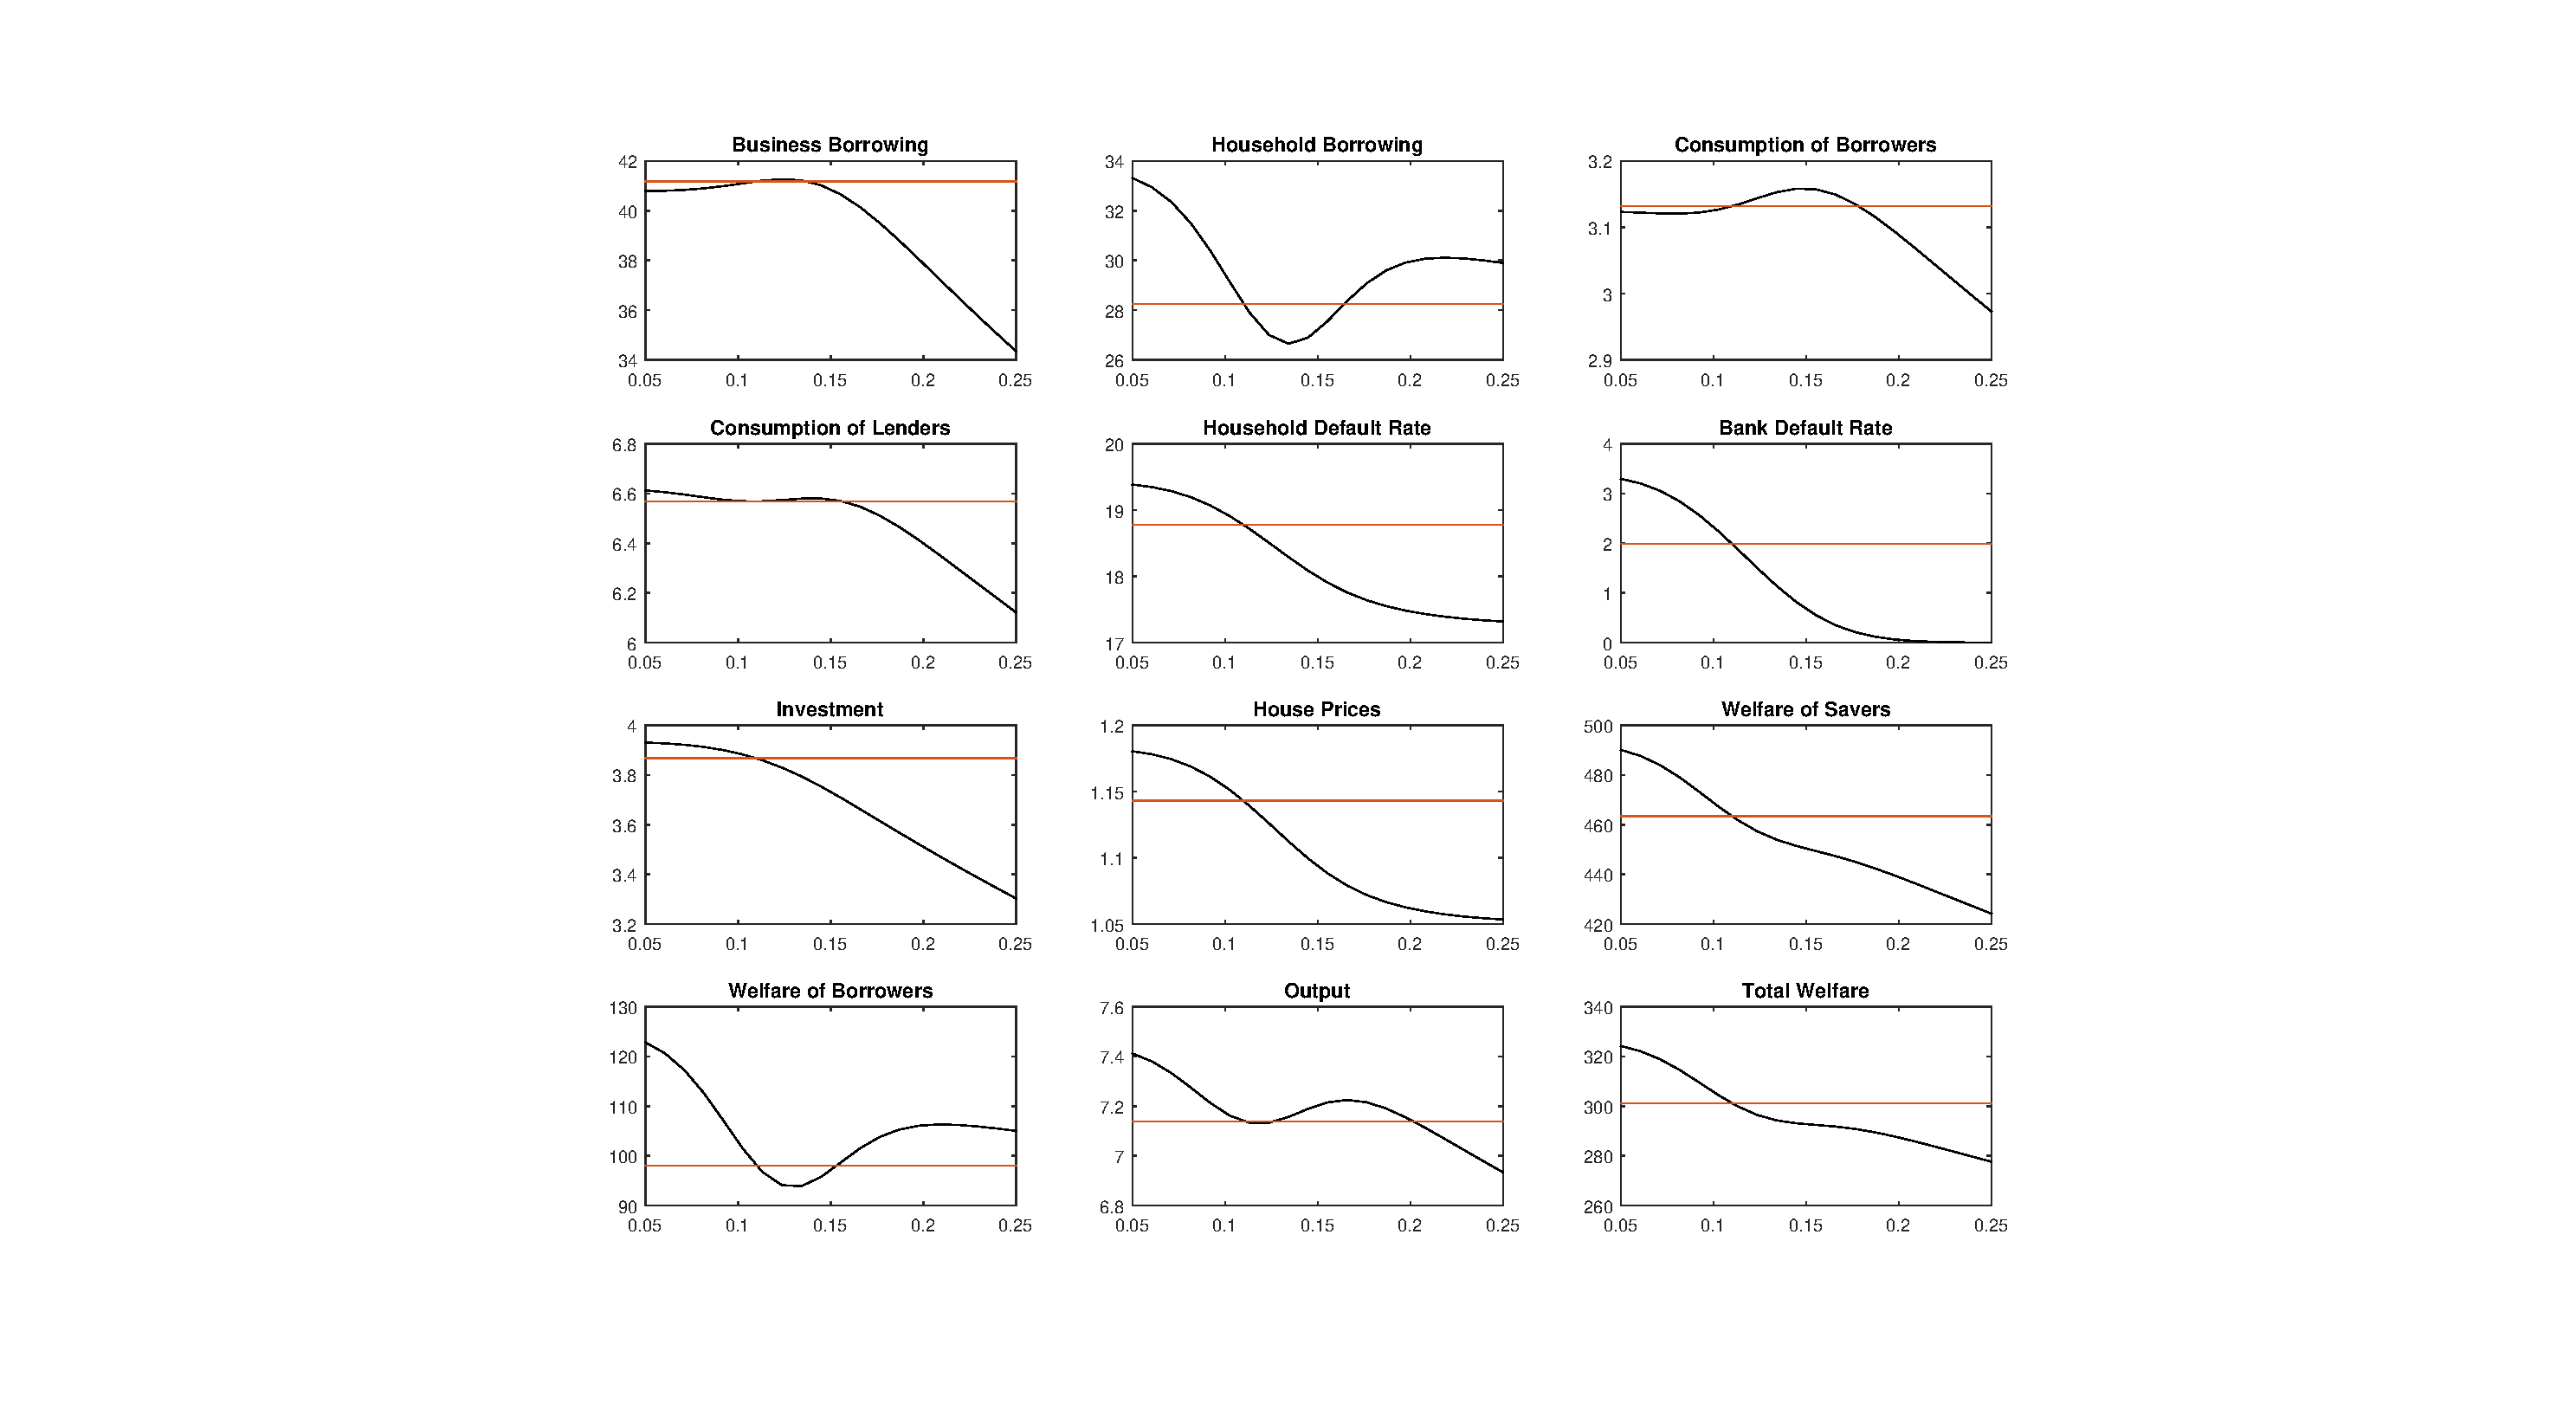
\includegraphics[scale=0.4]{WA3_var.pdf}
%\end{figure}


%\begin{figure}[H]
%\centering
%\caption{Minimum capital requirements with a baseline of 11\%. Welfare maximizing value is 15.5 \% with a weight of 0 on volatility. It decreases to 14.5 \% with a weight of 0.1 on volatility. 
%\textbf{Welfare improvement: 5.11 \% 3.82 \% respectively.} } 
%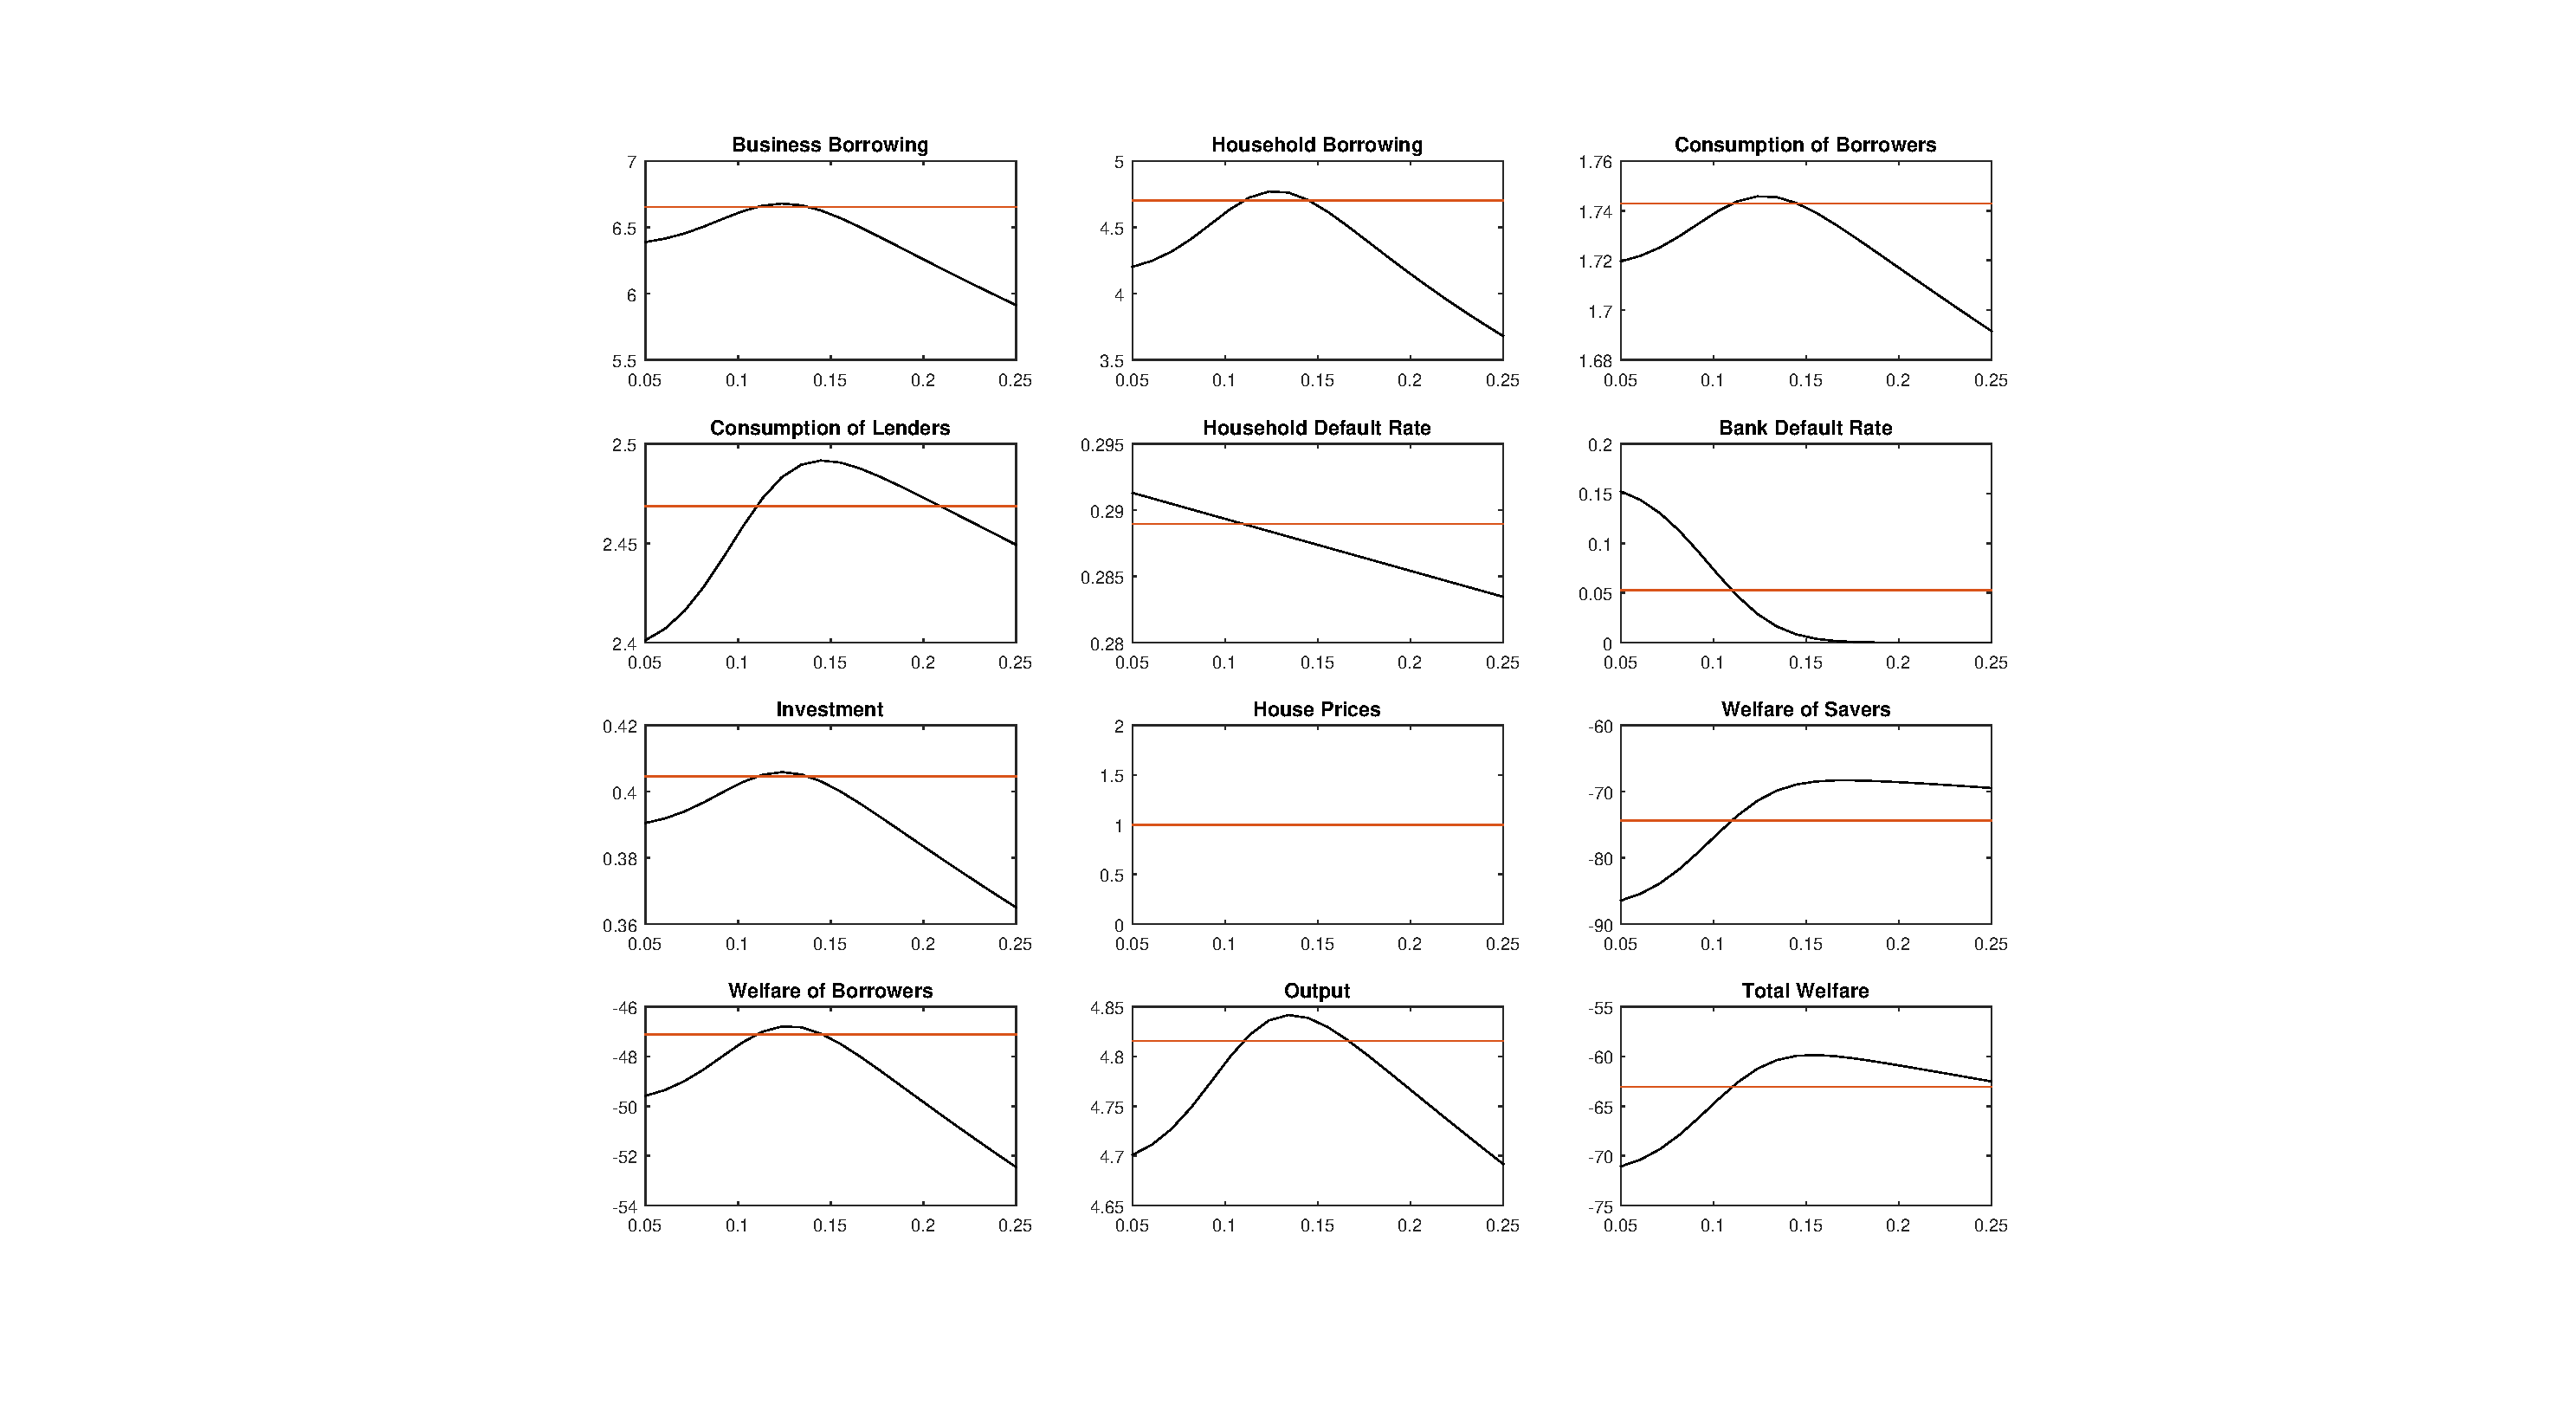
\includegraphics[scale=0.4]{WA4_level.pdf}\\
%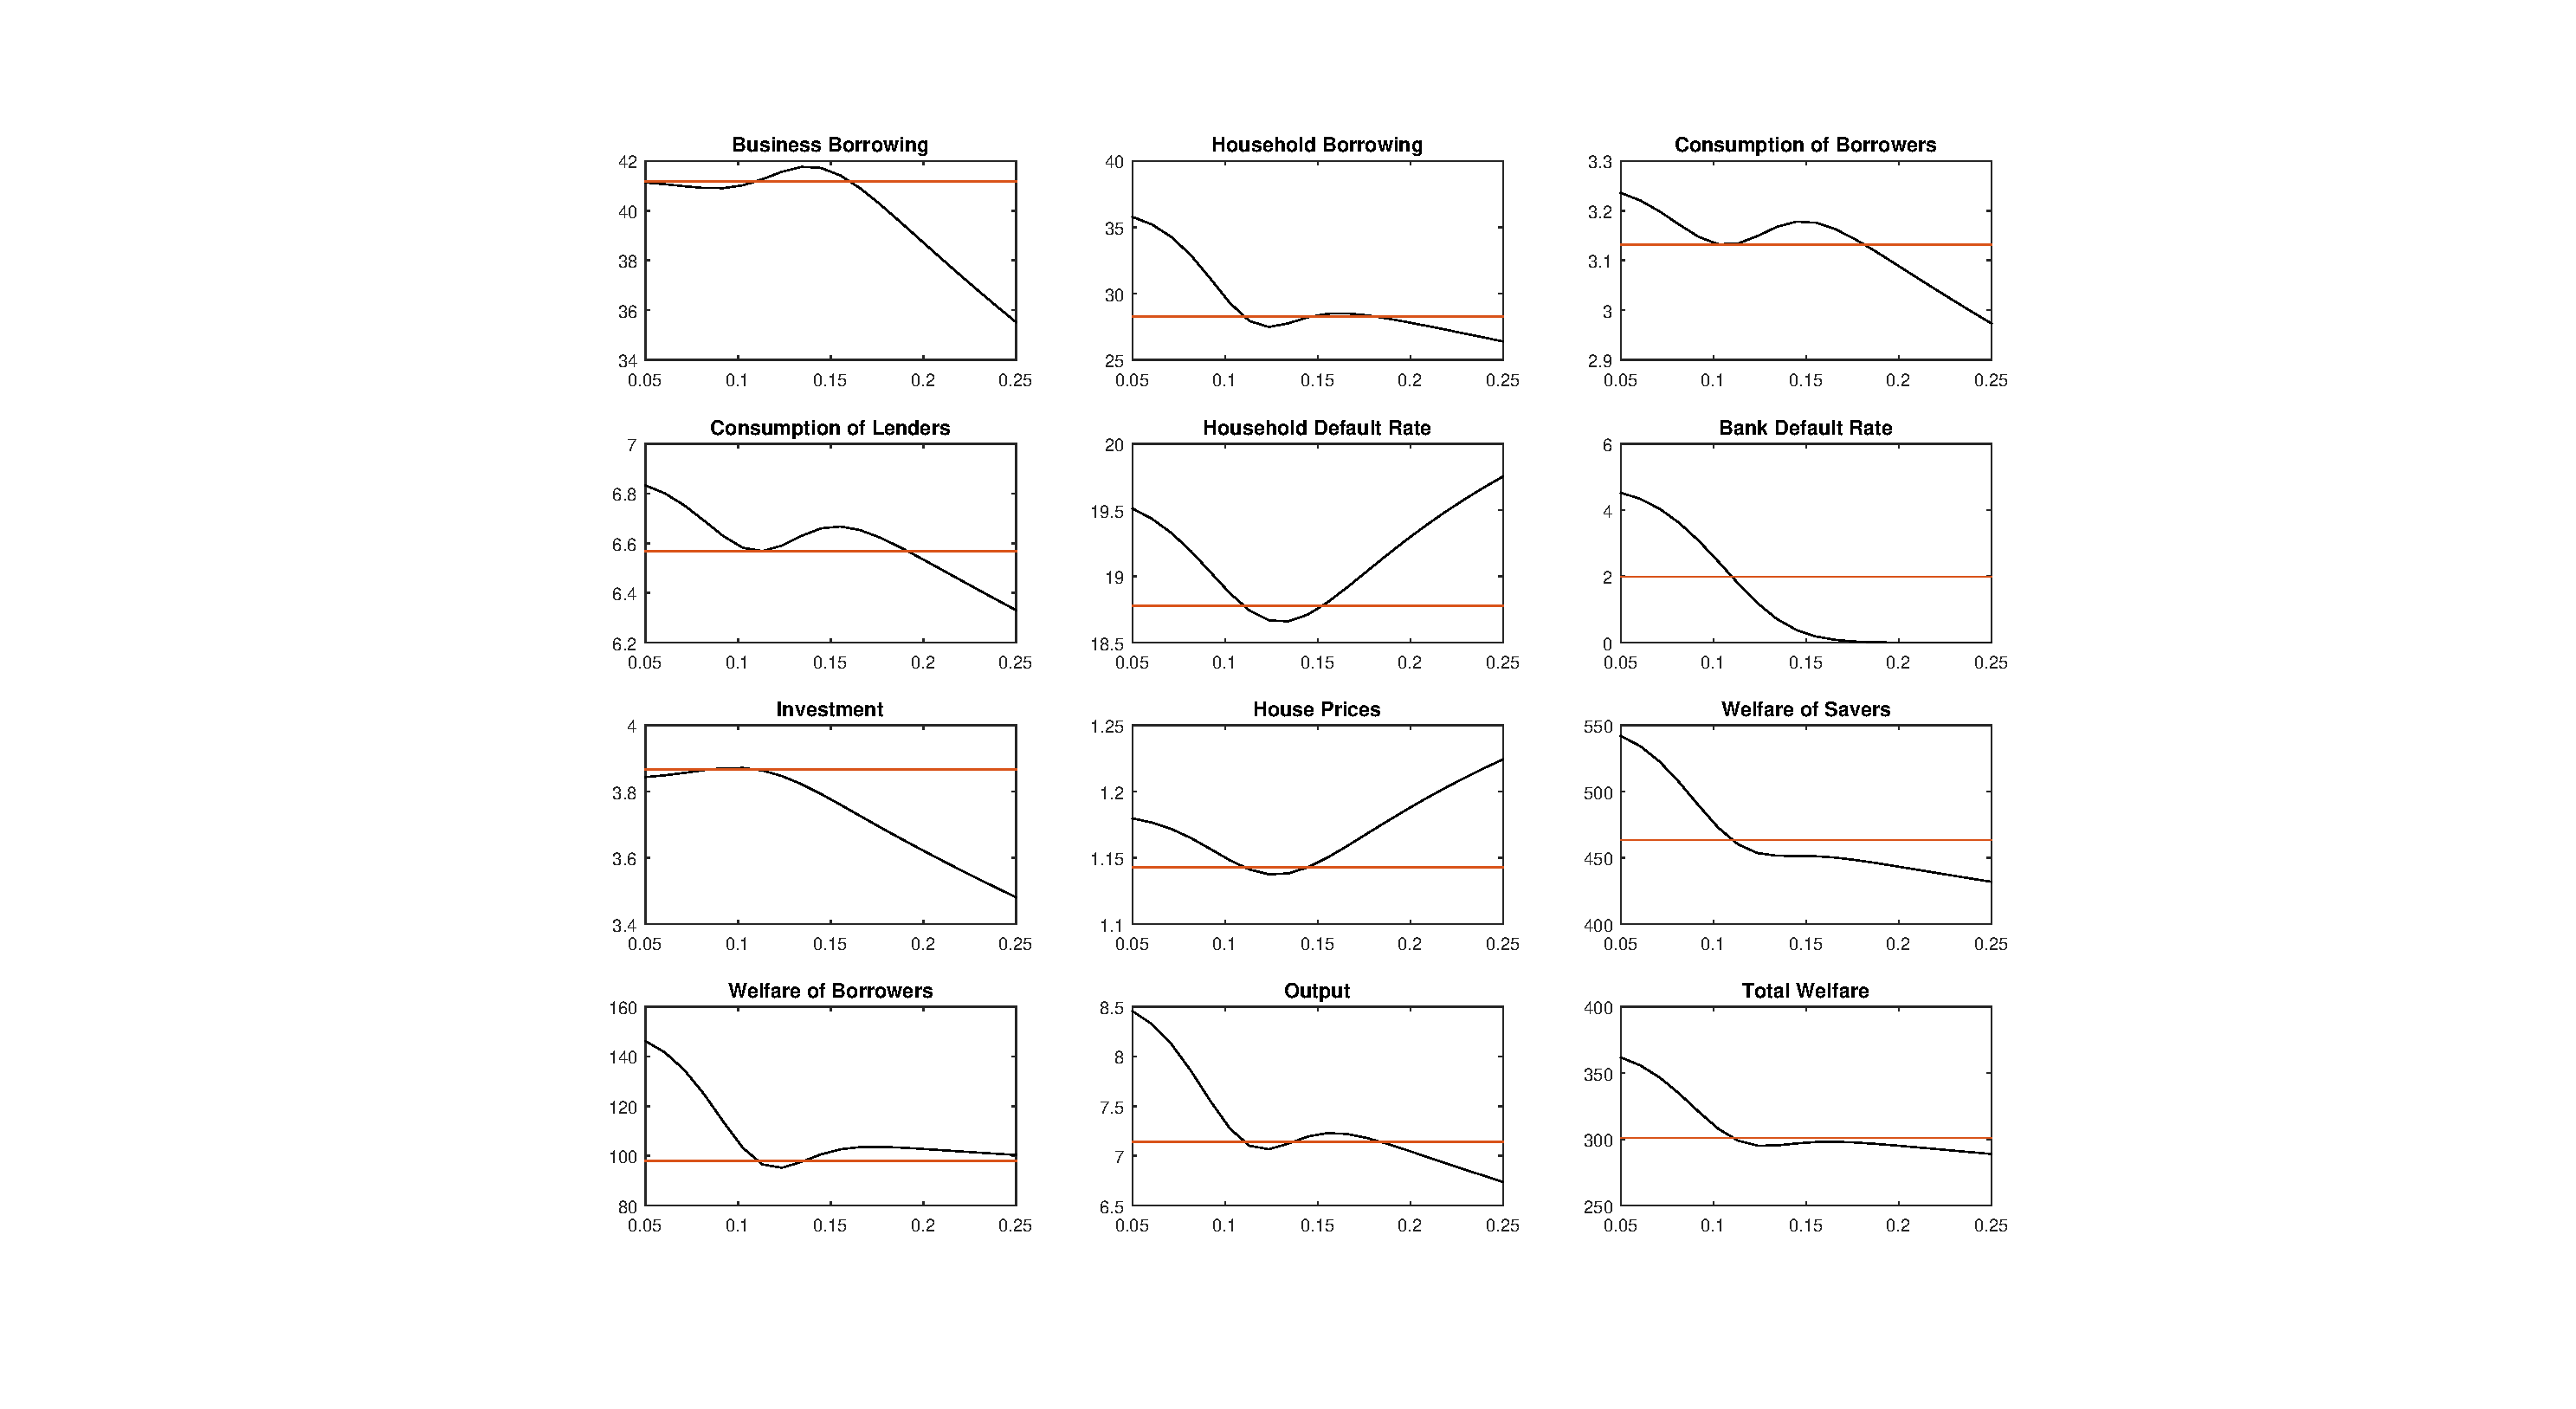
\includegraphics[scale=0.4]{WA4_var.pdf}
%\end{figure}





%\begin{figure}[H]
%\centering
%\caption{CCyB: this only affects the economy through volatility and not the levels. Therefore we only provide a positive analysis for this one in the counterfactuals but not optimize over its value: a linearized model is likely to give very imprecise results on this. 
%\textbf{Welfare improvement 0 with no weight on volatility, and 0.12 \% with a weight of 0.1 on volatility.} In the latter case it simply ends up at its maximum allowed value.} 
%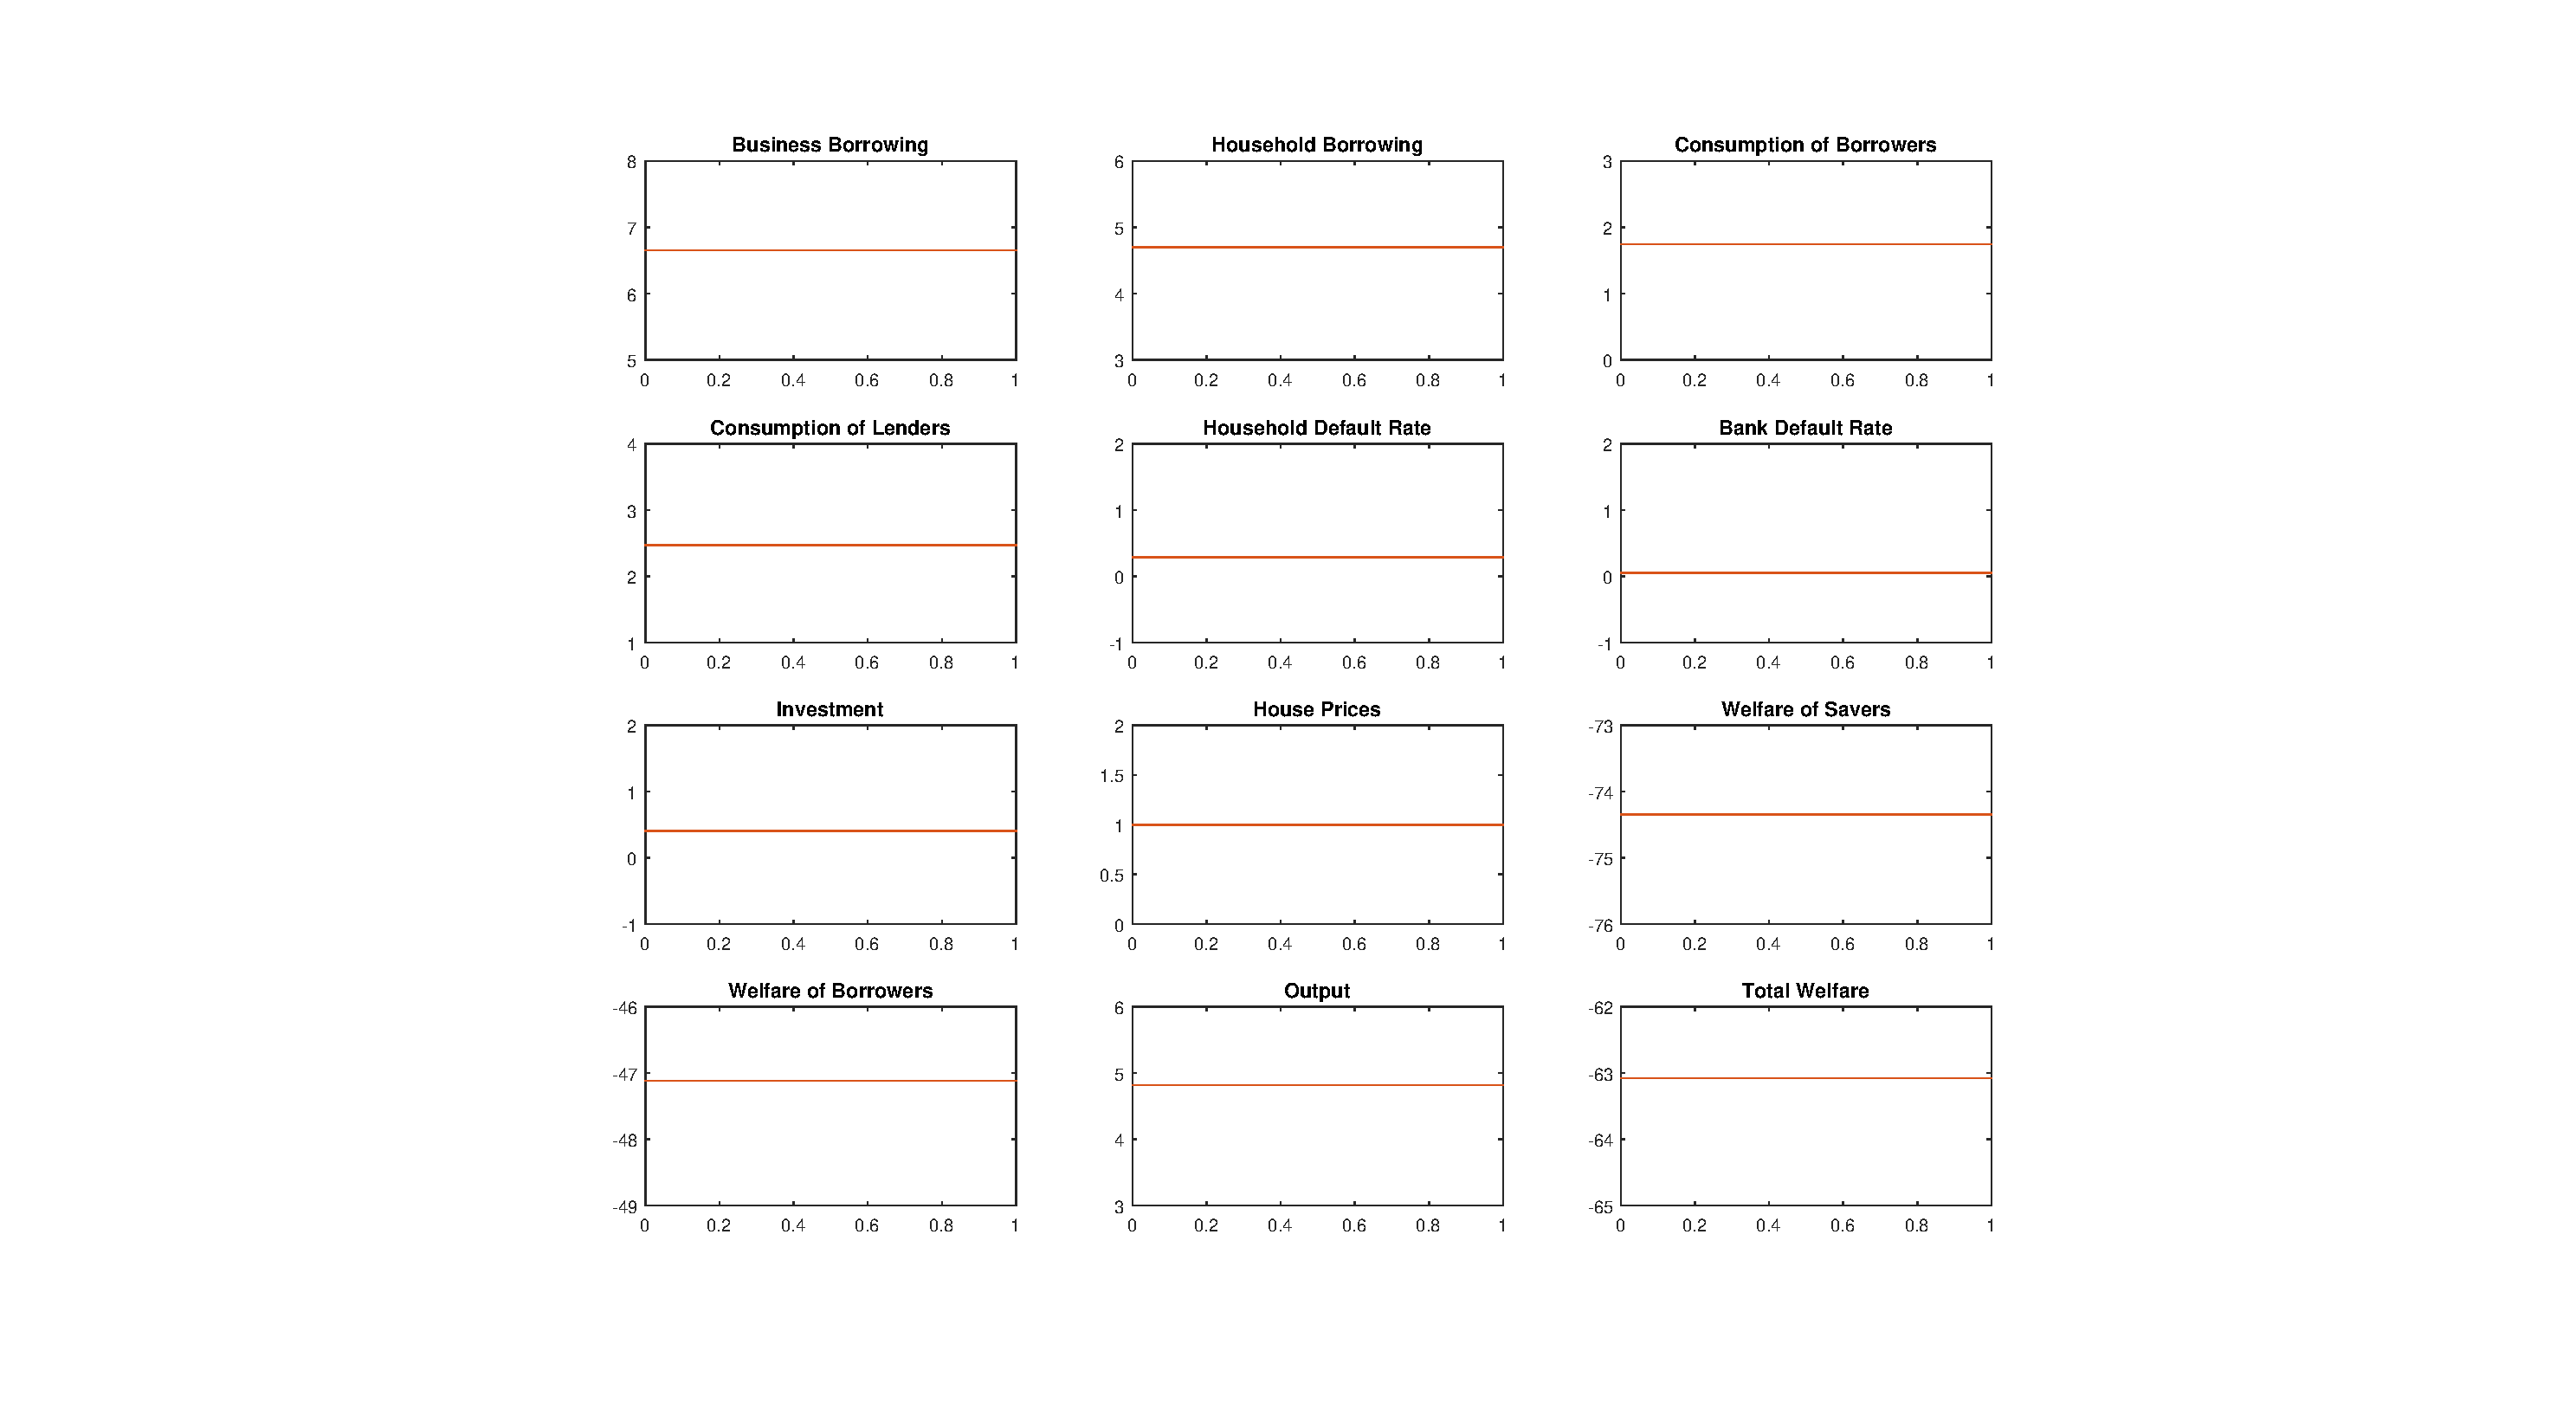
\includegraphics[scale=0.4]{WA5_level.pdf}\\
%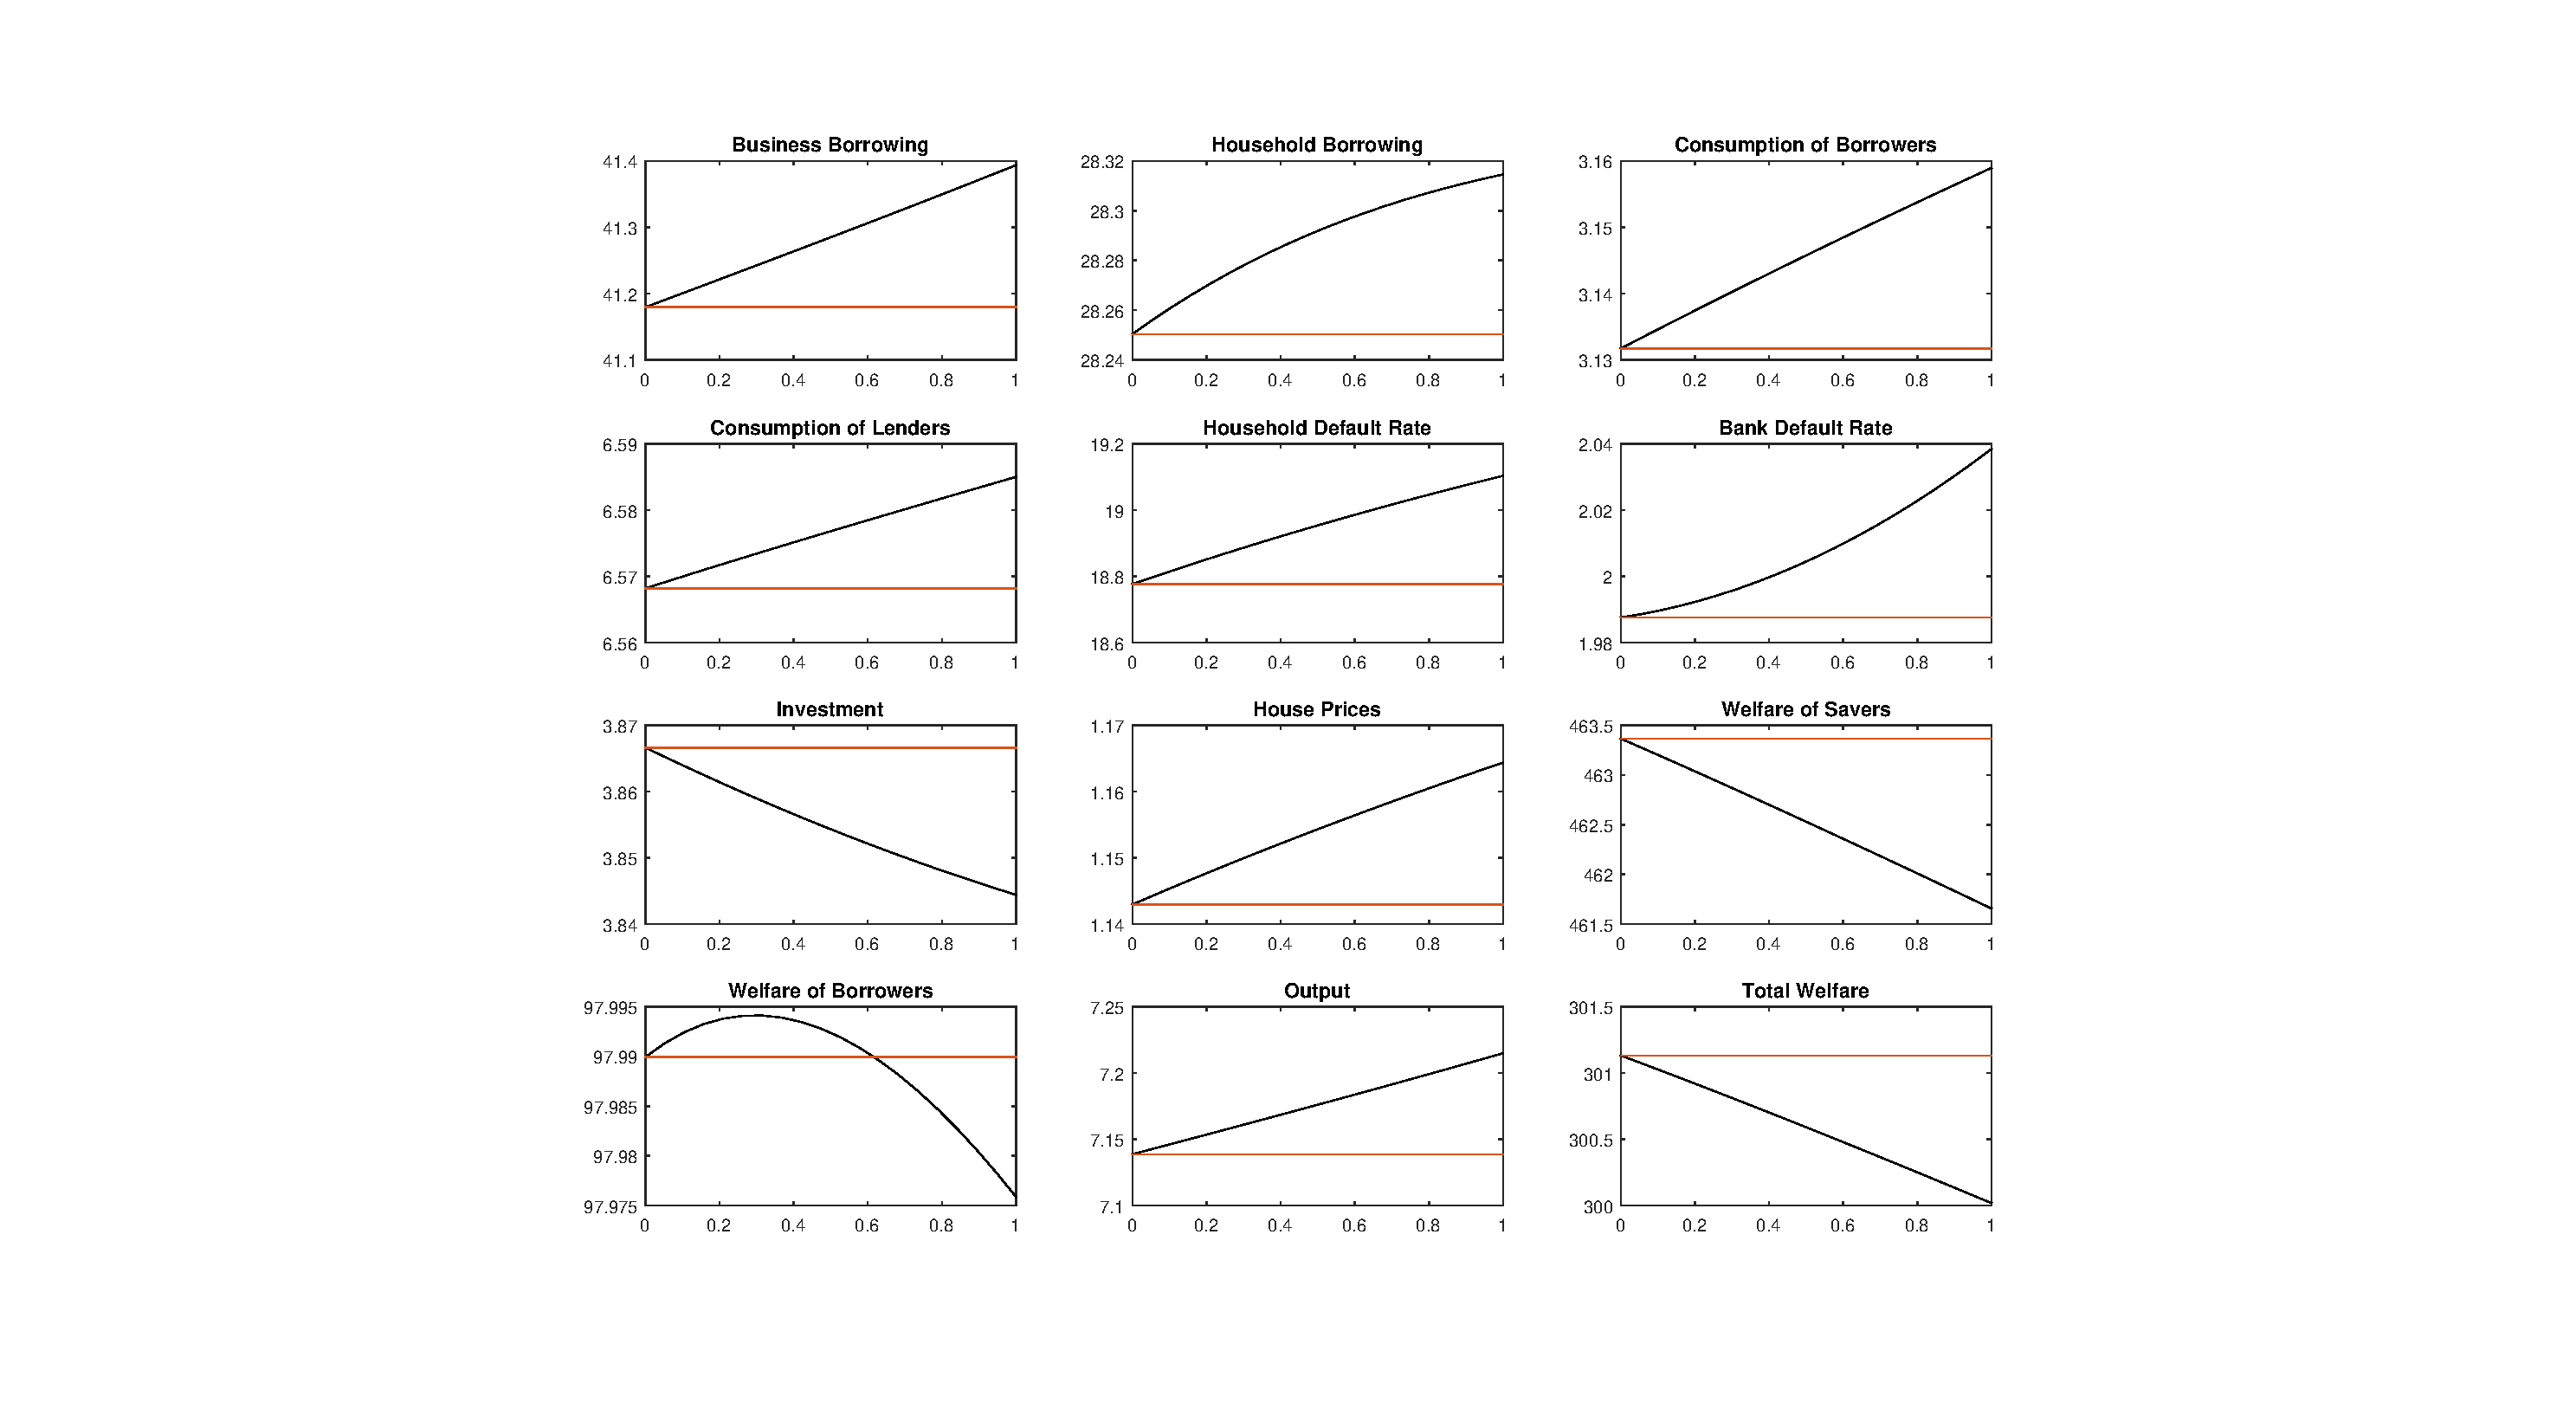
\includegraphics[scale=0.4]{WA5_var.pdf}
%\end{figure}



\section*{Optimal Minimum \& Sectoral Capital Requirements and LTV limit}

Objective function: 

$$ E[W_t] - \omega \sqrt{Var[W_t]} $$
where welfare $W_t$ is defined as a weighted average of patient and impatient households: 


$$ W_t = \frac{W^s_t C^s_t + W^m_t C^m_t}{C^s_t + C^m_t} $$

\begin{table}[h]

\caption{Maximizing over prudential policy parameters, one at a time.}
\label{optpolicy_table}
\begin{tabular}{l|l|l|l}

 & $\omega$ & 0 & 0.1   \\
 \hline
 \hline
Parameter & & &  \\
\hline
\hline
LTV &  & 89.4 \% (0.014 \%) & 86.6 \% (0.001 \%)  \\

SCR-Mortgage &  & 20.7 \% (7.47 \%) & 17.6 \% (4.26 \%) \\

SCR-Corporate & & 15.5 \% (3.33 \%) & 16.7 \% (3.22 \%) \\

CAR & & 15.5 \% (5.11 \%) & 14.5 \% (3.82 \%) \\

CCyB & & 0 \% (0 \%) & Max. attainable \\

\end{tabular}
\end{table}



\begin{table}[h]

\caption{Maximizing over SCRs and LTV at the same time}
\label{optpolicy_all}
\begin{tabular}{l|l|l|l}

 & $\omega$ & 0 & 0.1   \\
 \hline
 \hline
Parameter & & &  \\
\hline
\hline
LTV &  & 91.25 \%   &  94.06 \%  \\

SCR-Mortgage &  & 21.25 \%     & 15.88 \%   \\

SCR-Corporate & &  5(Min. attainable) \%  & 12.50 \%  \\

Welfare Improvement & & 8.01 \% & 4.8 \% \\

\end{tabular}
\end{table}





%\begin{figure}[h]
%\caption{Optimal policy values as a function of the weight on welfare volatility}
%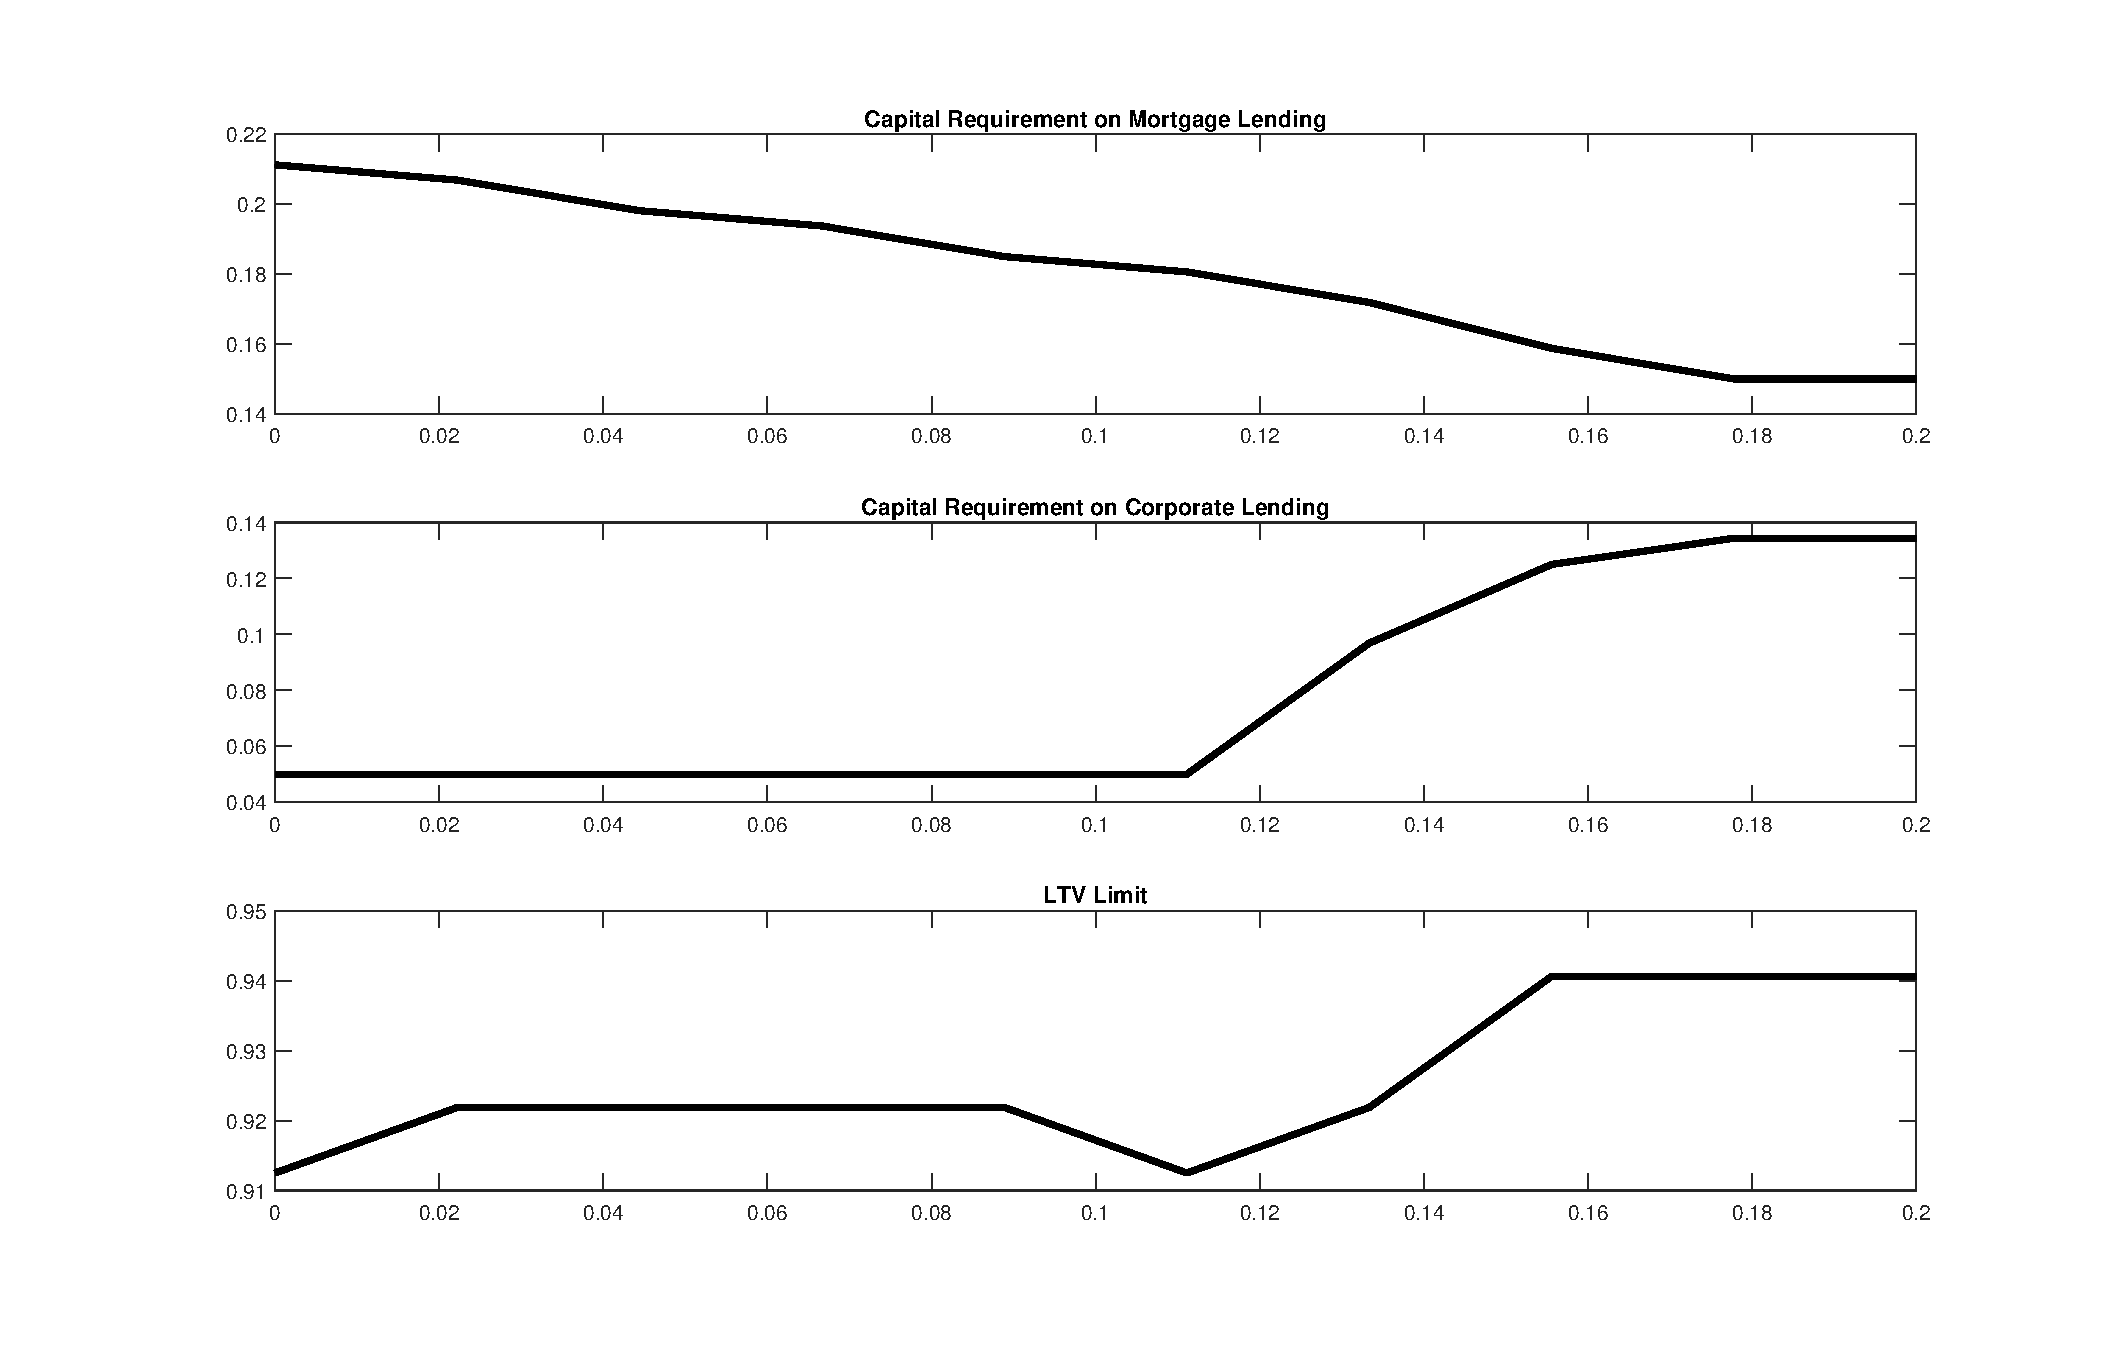
\includegraphics[scale=0.5]{optim_policy_values.pdf}
%\end{figure}



\newpage

\section*{Counterfactuals}


\begin{figure}[H]
\centering
\caption{Counterfactual I: using optimized values  with 0.1 weight on volatility. $\phi_H=15.8 \%, \phi_F=12.5 \%, \epsilon_H=94 \%$.}
\label{counterfact1_figure}
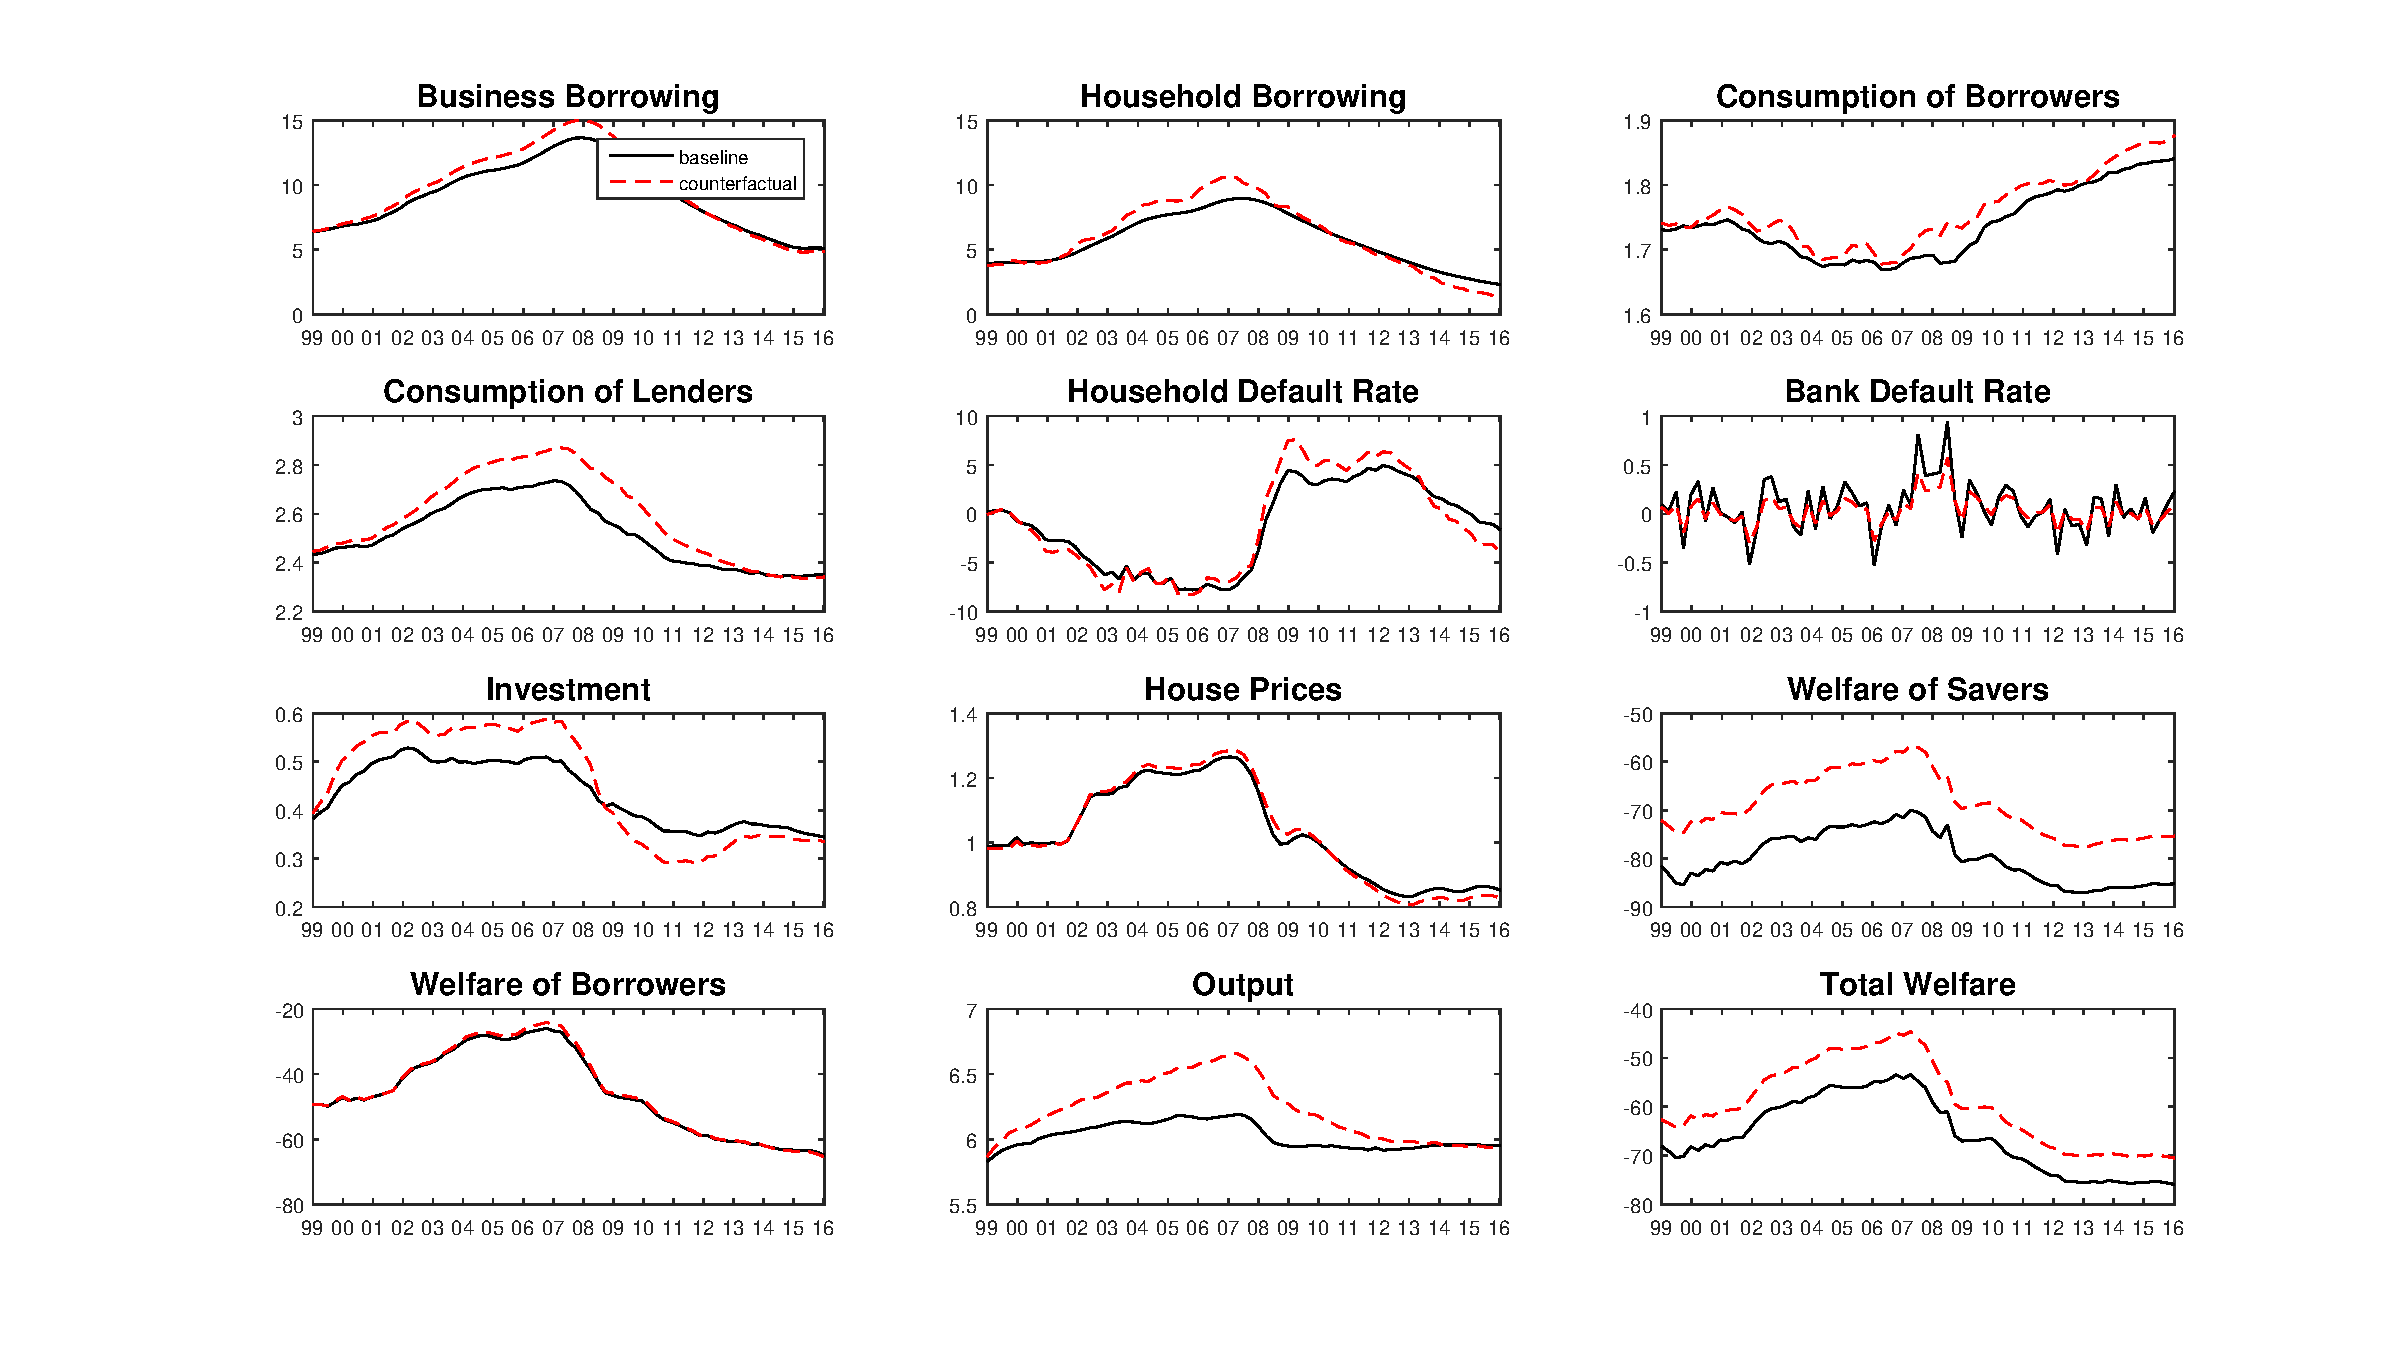
\includegraphics[scale=0.45]{counterfactuals2.pdf}
\end{figure}

\begin{table}[h]
\label{couterfac1_table}
\begin{tabular}{l|l|l}
Variable & \% Change in Level & \% Change in Volatility \\
\hline
\hline
    Corporate Credit           &       0.039    &      0.041 \\
    Mortgage Credit            &      0.024    &       0.147 \\
    Output         &     0.019    &    -0.354 \\ 
    Household Welfare       &     0.175     &     0.0437\\
\end{tabular}
\end{table}



\begin{figure}[H]
\centering
\caption{Same counterfactual phased-in over a 5-year period over 2001-2006 in equal increments.}
\label{counterfact2_figure}
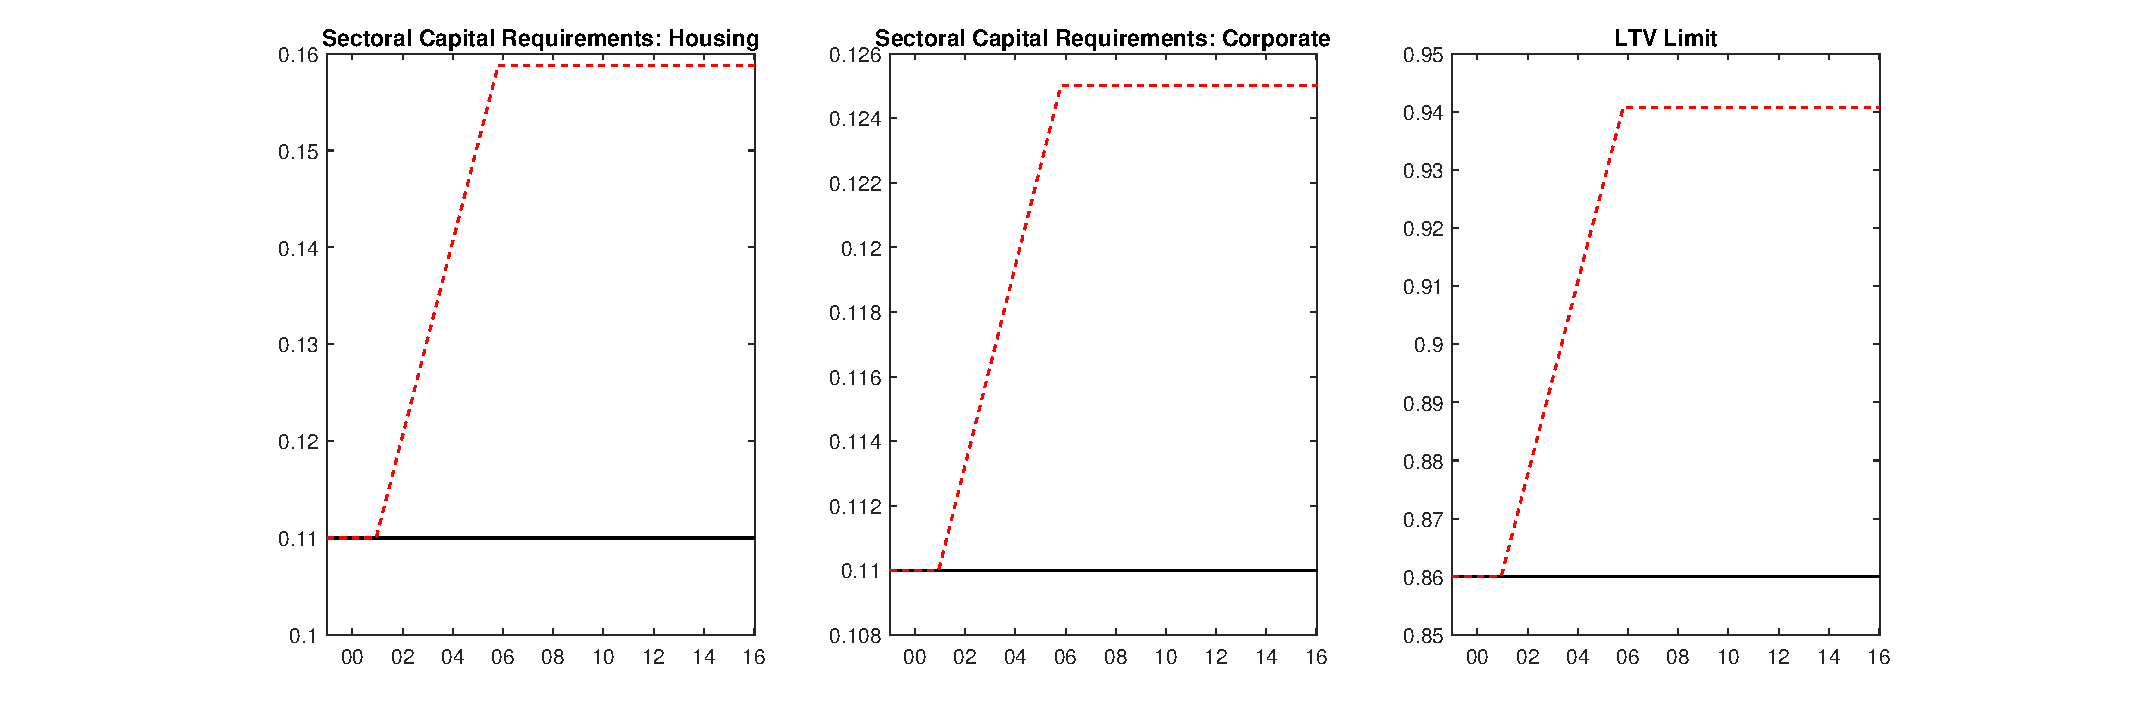
\includegraphics[scale=0.35]{CF_policy_rules10.pdf}
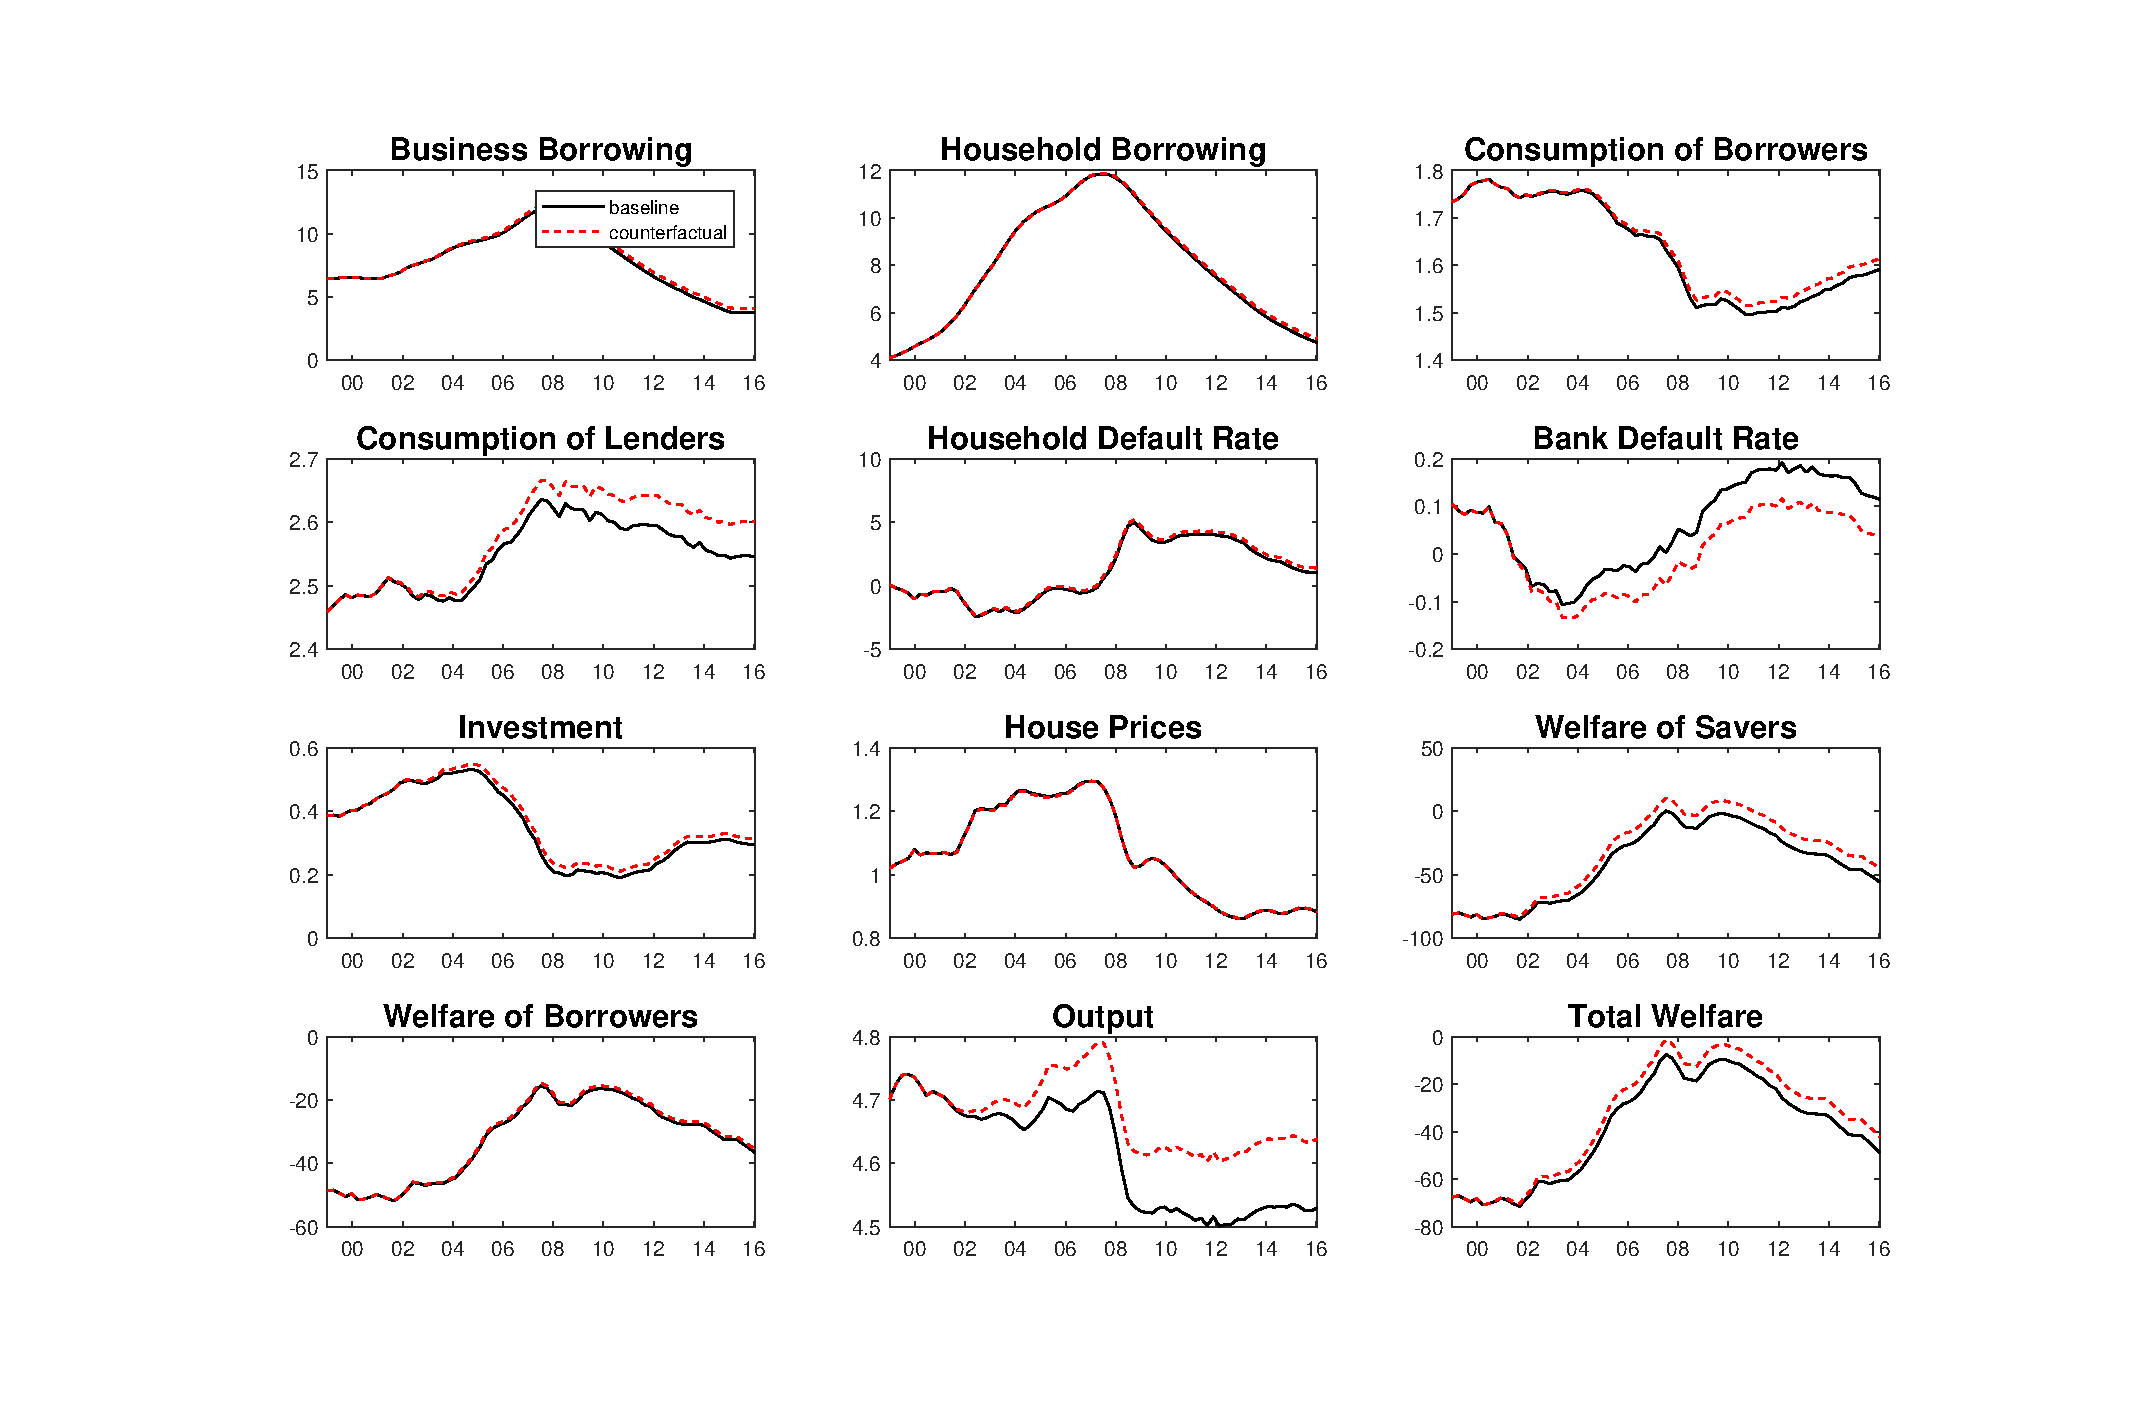
\includegraphics[scale=0.45]{counterfactuals10.pdf}\\

\end{figure}


\begin{table}[h]

\begin{tabular}{l|l|l}
\small
\label{counterfact2_table}
Variable & \% Change in Level & \% Change in Volatility \\
\hline
\hline
    Corporate Credit           &       0.024   &      -0.002 \\
    Mortgage Credit            &      0.007    &       -0.007 \\
    Output         				&     0.014    &    -0.359 \\ 
    Household Welfare       &     0.12     &     0.098\\
\end{tabular}
\end{table}



\begin{figure}[H]
\centering
\caption{Same counterfactual as above, without interest rate stickiness.}
\label{counterfact3_figure}
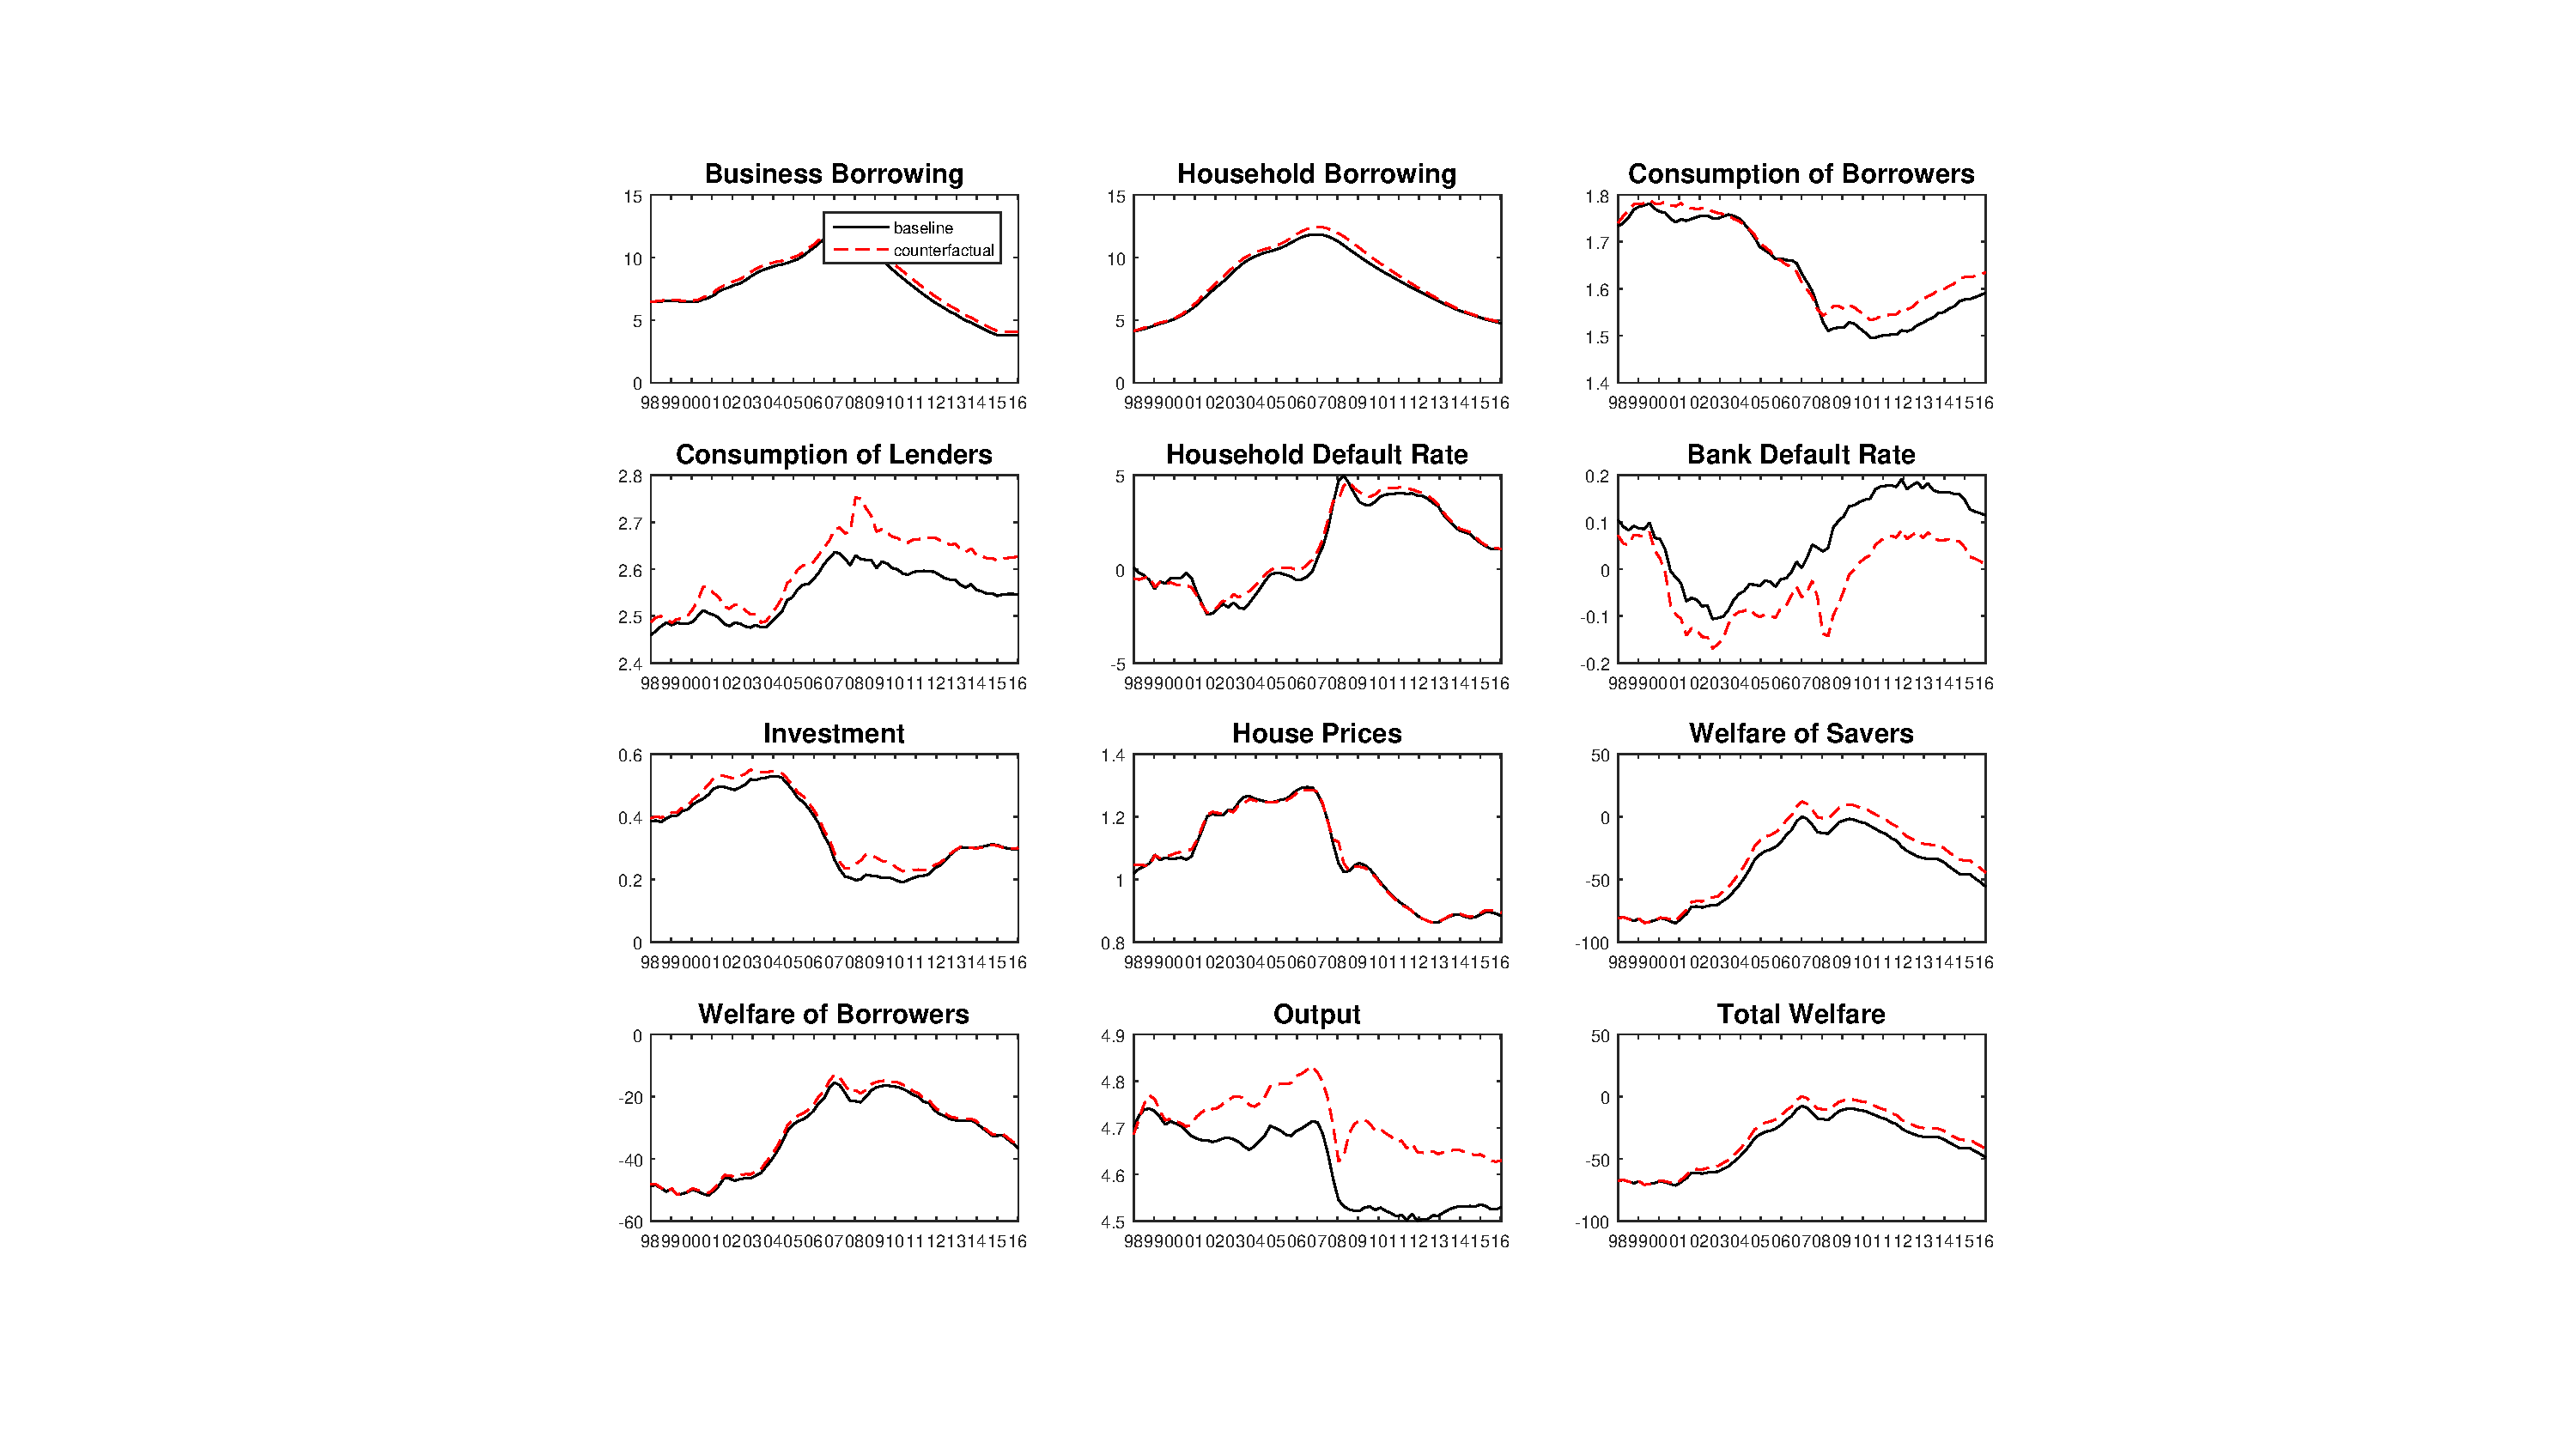
\includegraphics[scale=0.45]{counterfactuals11.pdf}
\end{figure}



\begin{table}[h]
\label{counterfact3_table}
\begin{tabular}{l|l|l}
\small
Variable & \% Change in Level & \% Change in Volatility \\
\hline
\hline
    Corporate Credit           &       0.041    &     0.003 \\
    Mortgage Credit            &      0.029    &      0.066 \\
    Output         				&     0.02    &    -0.29 \\ 
    Household Welfare       &     0.12     &     0.1\\
\end{tabular}
\end{table}






\begin{table}[h]
\label{counterfact_CCyB_table}
\caption{Does CCyB improve things when optimal SCRs are in place?}
\begin{tabular}{l|l|l}
\small
Variable & \% Change in Level & \% Change in Volatility \\
\hline
Baseline optimal SCR+LTV & & \\
\hline
    Corporate Credit           &       0.039    &      0.041 \\
    Mortgage Credit            &      0.024    &       0.147 \\
    Output         &     0.019    &    -0.354 \\ 
    Household Welfare       &     0.175     &     0.0437\\
\hline
CCyB 2.5 \%, both sectors & & \\
\hline
    Corporate Credit           &       0.045    &     0.074 \\
    Mortgage Credit            &      0.022    &      0.17 \\
    Output         				&     0.02    &    -0.055 \\ 
    Household Welfare       &     0.173     &     0.042\\
\hline
CCyB 2.5 \%, mortgages  & & \\
\hline
    Corporate Credit           &       0.039    &     0.074 \\
    Mortgage Credit            &      0.026    &      0.15 \\
    Output         				&     0.019    &    -0.098 \\ 
    Household Welfare       &     0.173     &     0.043\\
 \hline
CCyB 2.5 \%, corporate  & & \\
\hline
    Corporate Credit           &       0.045    &     0.041 \\
    Mortgage Credit            &      0.021    &      0.168 \\
    Output         				&     0.02    &    0.313 \\ 
    Household Welfare       &     0.175     &     0.0432\\   

\end{tabular}
\end{table}






\begin{comment}
cumulative differences with housing SCR

b_m_J =
   4.337368179975449
b_e_J =
   2.322443202268964
b_m_HD =
   3.226519809546808
b_m_ECAB =
   6.298439075960825
b_m_Hk =
   1.554806114474367
b_e_HD =
   0.384145956141740
b_e_ECAB =
   3.613437879492995
b_e_Hk =
   0.158518868370562


cumulative differences with housing LTV

b_m_J =
  -1.333054748265415
b_e_J =
   0.373505367214993
b_m_HD =
  -2.133692102030315
b_m_ECAB =
   3.730861575883666
b_m_Hk =
   0.074504326967662
b_e_HD =
   0.170076875628489
b_e_ECAB =
   0.690526482508227
b_e_Hk =
   0.202125249021339


CCyB


b_m_J =
  -0.273329733621980
b_e_J =
   0.195066050298801
b_m_HD =
   0.137436935811850
b_m_ECAB =
   2.543918366789851
b_m_Hk =
   4.604848115893450
b_e_HD =
   0.589361860281429
b_e_ECAB =
   1.399709895968916
b_e_Hk =
   1.442641082365731




\end{comment}








\begin{comment}
$bmHD =3.61   3.85, beHD =3.43   4.02$ ---- 0.24 0.59
$bmHD =11.94   9.81, beHD =0.68   0.85$---- -2.13 0.17
$bmHD =14.19  14.55,beHD =5.75   6.67$ ----  0.36 0.92
$bmECAB =2.2   5.1,beECAB =1.17   3.31$----  2.9   2.14
$bmECAB =5.19   8.93,beECAB =0.12   0.81$ --- 3.74 0.69
$bmECAB =47.95  52.78,beECAB =21.15  26.19$ ---- 4.83 5.04
\end{comment}

% phi_Hs=0.2112, phi_Fs=0.05, epsilonHs=0.89

%    'b_e'             7.84462528346059        8.67269308992684       0.10555861835901       2.4584010935864      2.74256603354155      0.115589331902144
%    'b_m'             7.95846777557005        7.56308146403059    -0.0496812103396544      2.49199646657523      2.84447642237499      0.141444805611695
%   'Y_net_2'         4.61389490762257        4.80998123121275     0.0424990875423346    0.0865850500268675    0.0699021998640299     -0.192675873694835
%    'welfare_'       -38.4431368247487       -27.0009840941536     0.297638373859985      21.3330310447274      22.8521781913702     0.0712110315434162



%same as above, phased in over a 5-year period: 

%	 'b_e'             7.84462528396997     8.30544497408816      0.0587433654810573      2.45840109362487      2.55491437083149      0.0392585560822045
%    'b_m'             7.95846777644759     7.52241274125662     -0.0547913301202823      2.49199646663593      2.42508972000822     -0.0268486522848193
%    'Y_net_2'         4.61389490771639     4.69694541913213      0.0180000873615149    0.0865850499954136    0.0534317858513725      -0.382898250284515
%    'welfare_'       -38.4431368143011    -35.7101015383757     0.0710929310770672      21.3330310487708       22.517287443649      0.0555128051035425




%same as above, no stickiness


 %   'b_e'             7.84462528396997      8.34949922478579      0.0643592169848451      2.45840109362487      2.50637048594057      0.0195124353141964
 %   'b_m'             7.95846777644759      7.56646723305889     -0.0492557806854219      2.49199646663593      2.60462094493635      0.0451944775236613
 %   'Y_net_2'         4.61389490771639       4.7082081674508      0.0204411373949339    0.0865850499954136    0.0604385712168193      -0.301974518464553
 %   'welfare_'       -38.4431368143011     -36.1965521230706     0.0584391617698275      21.3330310487708      22.3768819478318        0.04893120422853









\begin{comment}


\begin{figure}[H]
\centering
\caption{optimized values with no weight on volatility: phiH=0.21, phiF=0.05, epsilonH=0.89 }
\includegraphics[scale=0.45]{counterfactuals1.pdf}
\end{figure}



\begin{figure}[H]
\centering
\caption{optimized values with 0.1 weight on volatility: phiH=0.158, phiF=0.125, epsilonH=0.94 }
\includegraphics[scale=0.45]{counterfactuals2.pdf}
\end{figure}



\begin{figure}[H]
\centering
\caption{same as above with CCyB=0.5 }
\includegraphics[scale=0.45]{counterfactuals3.pdf}
\end{figure}


%nothing on 4

\begin{figure}[H]
\centering
\caption{stickiness vs no stickiness}
\includegraphics[scale=0.45]{counterfactuals5.pdf}
\end{figure}


\begin{figure}[H]
\centering
\caption{CCyB=0.5 in the baseline version}
\includegraphics[scale=0.45]{counterfactuals6.pdf}
\end{figure}


\begin{figure}[H]
\centering
\caption{CCyB=0.5 in the baseline version without stickiness}
\includegraphics[scale=0.45]{counterfactuals7.pdf}
\end{figure}

\begin{figure}[H]
\centering
\caption{same as the CF1, phased-in over a 5-year period}
\includegraphics[scale=0.45]{counterfactuals8.pdf}\\
\includegraphics[scale=0.45]{CF_policy_rules8.pdf}
\end{figure}



\begin{figure}[H]
\centering
\caption{same as above, with no stickiness}
\includegraphics[scale=0.45]{counterfactuals9.pdf}
\end{figure}


\begin{figure}[H]
\centering
\caption{same as CF2, phased-in over a 5-year period}
\includegraphics[scale=0.45]{counterfactuals10.pdf}\\
\includegraphics[scale=0.45]{CF_policy_rules10.pdf}
\end{figure}


\begin{figure}[H]
\centering
\caption{same as above, no stickiness}
\includegraphics[scale=0.45]{counterfactuals11.pdf}
\end{figure}


\end{comment}


\begin{comment}
\begin{lstlisting}

CF1

 phi_Hs=0.2112, phi_Fs=0.05, epsilonHs=0.89


    'b_e'             7.8446           8.6727     2.4584          2.7426
    'b_m'             7.9585           7.5631      2.492          2.8445
    'C_m'             1.6351           1.6395     0.1043          0.0828
    'C_s'             2.5485           2.6781     0.0534          0.0741
    'def_rate_m'      1.0384           1.3593     2.2305          2.5238
    'def_rate_B'      0.0622          -0.0054     0.0932          0.0155
    'I'               0.3498             0.39     0.1162          0.1198
    'q_H'             1.0684           1.0722     0.1485          0.1721
    'Vs'            -41.1369         -21.4746    28.7173         30.4658
    'Vm'            -32.6029         -33.9885    12.3896         12.4668
    'Y_net_2'         4.6139             4.81     0.0866          0.0699
    'welfare_'      -38.4431          -27.001     21.333         22.8522

same as above, phased in over a 5-year period: 

    'b_e'             7.8446           8.3053     2.4584          2.5548
    'b_m'             7.9585           7.5234      2.492          2.4229
    'C_m'             1.6351           1.6591     0.1043           0.087
    'C_s'             2.5485           2.5922     0.0534          0.0791
    'def_rate_m'      1.0384           1.1172     2.2305          2.2008
    'def_rate_B'      0.0622           0.0405     0.0932           0.097
    'I'               0.3498           0.3821     0.1162          0.1158
    'q_H'             1.0684           1.0655     0.1485          0.1442
    'Vs'            -41.1369          -35.196    28.7173         31.3178
    'Vm'            -32.6029         -34.2851    12.3896         11.6184
    'Y_net_2'         4.6139           4.6967     0.0866          0.0534
    'welfare_'      -38.4431         -35.7081     21.333         22.5171

same as above, no stickiness

    'b_e'             7.8446           8.3419     2.4584          2.5126
    'b_m'             7.9585           7.5669      2.492          2.5516
    'C_m'             1.6351            1.664     0.1043          0.0877
    'C_s'             2.5485           2.6004     0.0534           0.077
    'def_rate_m'      1.0384           1.0908     2.2305          2.0888
    'def_rate_B'      0.0622           0.0329     0.0932          0.0966
    'I'               0.3498            0.382     0.1162          0.1163
    'q_H'             1.0684           1.0663     0.1485          0.1414
    'Vs'            -41.1369         -35.8384    28.7173         31.1584
    'Vm'            -32.6029         -34.5019    12.3896         11.5105
    'Y_net_2'         4.6139           4.7064     0.0866          0.0602
    'welfare_'      -38.4431         -36.1781     21.333         22.3638    


stickiness vs. no stickiness in the baseline, for comparison


        field_names     baseline_mean    cf_mean     baseline_var    cf_var 
    ____________    _____________    ________    ____________    _______

    'b_e'             7.8446           7.9368     2.4584          2.4669
    'b_m'             7.9585           8.0879      2.492          2.6615
    'C_m'             1.6351           1.6442     0.1043          0.1026
    'C_s'             2.5485           2.5659     0.0534          0.0568
    'def_rate_m'      1.0384           1.0151     2.2305          2.1398
    'def_rate_B'      0.0622           0.0457     0.0932          0.0971
    'I'               0.3498           0.3525     0.1162          0.1205
    'q_H'             1.0684           1.0705     0.1485          0.1472
    'Vs'            -41.1369          -41.465    28.7173         28.7003
    'Vm'            -32.6029         -32.5926    12.3896         12.3201
    'Y_net_2'         4.6139           4.6354     0.0866           0.095
    'welfare_'      -38.4431         -38.6465     21.333         21.2902



%===============================================================================================
CF2

 phi_Hs=0.158, phi_Fs=0.125, epsilonHs=0.94

    'b_e'             7.8446           8.1534     2.4584          2.5586
    'b_m'             7.9585           8.1513      2.492          2.8605
    'C_m'             1.6351           1.6408     0.1043          0.1025
    'C_s'             2.5485           2.6098     0.0534          0.0664
    'def_rate_m'      1.0384           1.7747     2.2305          2.7548
    'def_rate_B'      0.0622           0.0247     0.0932            0.05
    'I'               0.3498            0.365     0.1162          0.1149
    'q_H'             1.0684           1.0708     0.1485          0.1564
    'Vs'            -41.1369         -30.2546    28.7173         29.5883
    'Vm'            -32.6029         -32.2776    12.3896         12.9986
    'Y_net_2'         4.6139           4.7017     0.0866          0.0559
    'welfare_'      -38.4431          -31.705     21.333         22.2655

 


CF3

CF2+ CCyb=0.5--> CCyB such that the standard deviation of  



    'b_e'             7.8446           8.1906     2.4584          2.6709
    'b_m'             7.9585           8.1436      2.492          2.9029
    'C_m'             1.6351           1.6427     0.1043          0.1095
    'C_s'             2.5485           2.6128     0.0534          0.0644
    'def_rate_m'      1.0384           1.8184     2.2305          3.0709
    'def_rate_B'      0.0622           0.0254     0.0932          0.0926
    'I'               0.3498           0.3636     0.1162          0.1251
    'q_H'             1.0684           1.0718     0.1485          0.1614
    'Vs'            -41.1369          -30.477    28.7173          29.488
    'Vm'            -32.6029         -32.2094    12.3896         13.0924
    'Y_net_2'         4.6139           4.7055     0.0866          0.0885
    'welfare_'      -38.4431         -31.8079     21.333         22.2409


    (when I repeat with CF1 + CCyB=0.2, indeterminacy)





    CF5 estimated stickiness vs small stickiness


        field_names     baseline_mean    cf_mean     baseline_var    cf_var 
    ____________    _____________    ________    ____________    _______

    'b_e'             7.8446           7.9368     2.4584          2.4669
    'b_m'             7.9585           8.0879      2.492          2.6615
    'C_m'             1.6351           1.6442     0.1043          0.1026
    'C_s'             2.5485           2.5659     0.0534          0.0568
    'def_rate_m'      1.0384           1.0151     2.2305          2.1398
    'def_rate_B'      0.0622           0.0457     0.0932          0.0971
    'I'               0.3498           0.3525     0.1162          0.1205
    'q_H'             1.0684           1.0705     0.1485          0.1472
    'Vs'            -41.1369          -41.465    28.7173         28.7003
    'Vm'            -32.6029         -32.5926    12.3896         12.3201
    'Y_net_2'         4.6139           4.6354     0.0866           0.095
    'welfare_'      -38.4431         -38.6465     21.333         21.2902




CF6 CCyB=0.5 in the baseline case 


    'b_e'             7.8446           7.8953     2.4584          2.5634
    'b_m'             7.9585           7.9674      2.492          2.5526
    'C_m'             1.6351           1.6389     0.1043          0.1052
    'C_s'             2.5485           2.5548     0.0534          0.0548
    'def_rate_m'      1.0384           1.0477     2.2305          2.2942
    'def_rate_B'      0.0622           0.0598     0.0932           0.136
    'I'               0.3498           0.3491     0.1162          0.1234
    'q_H'             1.0684           1.0695     0.1485           0.152
    'Vs'            -41.1369         -41.3159    28.7173         28.6433
    'Vm'            -32.6029         -32.6482    12.3896         12.3391
    'Y_net_2'         4.6139           4.6216     0.0866           0.119
    'welfare_'      -38.4431         -38.5701     21.333         21.2774


    CF7 CCyB=0.5 in baseline without stickiness

    'b_e'             7.8446           7.9679     2.4584          2.6461
    'b_m'             7.9585            8.052      2.492          2.7172
    'C_m'             1.6351           1.6474     0.1043          0.1091
    'C_s'             2.5485           2.5693     0.0534          0.0552
    'def_rate_m'      1.0384           1.0312     2.2305          2.2725
    'def_rate_B'      0.0622           0.0477     0.0932          0.1536
    'I'               0.3498           0.3489     0.1162          0.1355
    'q_H'             1.0684           1.0717     0.1485          0.1534
    'Vs'            -41.1369         -41.7983    28.7173         28.5386
    'Vm'            -32.6029         -32.7987    12.3896         12.1343
    'Y_net_2'         4.6139           4.6364     0.0866          0.1453
    'welfare_'      -38.4431         -38.9232     21.333         21.1367


CF8: CF1 with 5-year phasing in


    'b_e'             7.8446           8.3053     2.4584          2.5548
    'b_m'             7.9585           7.5234      2.492          2.4229
    'C_m'             1.6351           1.6591     0.1043           0.087
    'C_s'             2.5485           2.5922     0.0534          0.0791
    'def_rate_m'      1.0384           1.1172     2.2305          2.2008
    'def_rate_B'      0.0622           0.0405     0.0932           0.097
    'I'               0.3498           0.3821     0.1162          0.1158
    'q_H'             1.0684           1.0655     0.1485          0.1442
    'Vs'            -41.1369          -35.196    28.7173         31.3178
    'Vm'            -32.6029         -34.2851    12.3896         11.6184
    'Y_net_2'         4.6139           4.6967     0.0866          0.0534
    'welfare_'      -38.4431         -35.7081     21.333         22.5171



CF9: same as above, without stickiness


    'b_e'             7.8446           8.3419     2.4584          2.5126
    'b_m'             7.9585           7.5669      2.492          2.5516
    'C_m'             1.6351            1.664     0.1043          0.0877
    'C_s'             2.5485           2.6004     0.0534           0.077
    'def_rate_m'      1.0384           1.0908     2.2305          2.0888
    'def_rate_B'      0.0622           0.0329     0.0932          0.0966
    'I'               0.3498            0.382     0.1162          0.1163
    'q_H'             1.0684           1.0663     0.1485          0.1414
    'Vs'            -41.1369         -35.8384    28.7173         31.1584
    'Vm'            -32.6029         -34.5019    12.3896         11.5105
    'Y_net_2'         4.6139           4.7064     0.0866          0.0602
    'welfare_'      -38.4431         -36.1781     21.333         22.3638


CF10: CF2 with 5-year phasing in


    'b_e'             7.8446           8.0296     2.4584          2.4432
    'b_m'             7.9585           8.0715      2.492          2.4814
    'C_m'             1.6351           1.6464     0.1043          0.0961
    'C_s'             2.5485           2.5769     0.0534          0.0699
    'def_rate_m'      1.0384           1.2165     2.2305          2.3175
    'def_rate_B'      0.0622           0.0023     0.0932          0.0809
    'I'               0.3498           0.3649     0.1162          0.1107
    'q_H'             1.0684           1.0683     0.1485          0.1471
    'Vs'            -41.1369         -32.5114    28.7173          32.548
    'Vm'            -32.6029         -31.6476    12.3896         12.8566
    'Y_net_2'         4.6139           4.6818     0.0866          0.0534
    'welfare_'      -38.4431         -33.0516     21.333          23.738


CF11: same as above, without stickiness

    'b_e'             7.8446           8.1684     2.4584          2.4622
    'b_m'             7.9585           8.2669      2.492           2.673
    'C_m'             1.6351           1.6583     0.1043           0.092
    'C_s'             2.5485           2.6018     0.0534          0.0754
    'def_rate_m'      1.0384           1.1964     2.2305          2.2341
    'def_rate_B'      0.0622          -0.0217     0.0932          0.0811
    'I'               0.3498           0.3707     0.1162          0.1146
    'q_H'             1.0684           1.0711     0.1485          0.1463
    'Vs'            -41.1369         -32.4889    28.7173         32.6665
    'Vm'            -32.6029         -31.4009    12.3896         12.8785
    'Y_net_2'         4.6139           4.7139     0.0866          0.0583
    'welfare_'      -38.4431         -32.9639     21.333         23.8076


\end{lstlisting}
\end{comment}


\begin{comment}

\begin{figure}[H]
\centering
\caption{10 \% drop in LTV for household: all target variables decrease (output and borrowing) but results on welfare are ambiguous. Borrowers are slightly better off, because they can spend their money on consumption instead of housing (and probably work less). Lending households are worse off since both types of lending are reduced (less demand --> lower interest rates). 
}
\includegraphics[scale=0.45]{counterfactuals1.pdf}
\end{figure}

\begin{table}[H]
%\tiny
\begin{tabular}{l|l|l}
Variable & Mean under Baseline & Mean under Counterfactual \\ 
\hline
\hline
Business Credit  & 7.58 & 7.56 \\
Household Credit & 11.06 & 10.34 \\
Output & 5.94 & 5.91 \\
Lenders' Welfare & -32.13 & -34.22 \\
Borrowers' Welfare  & -25.03 & -23.13 \\
\end{tabular}
\end{table}

\begin{comment}
\begin{lstlisting}
    'b_e'             7.8446           7.8321      6.0437          6.0353
    'b_m'             7.9585           7.5392        6.21          4.2734
    'C_m'             1.6351           1.6502      0.0109          0.0083
    'C_s'             2.5485           2.5349      0.0029          0.0019
    'def_rate_m'      1.0384           0.1105       4.975          0.6186
    'def_rate_B'      0.0622           0.0622      0.0087          0.0078
    'Vs'            -41.1369         -41.7883    824.6828        817.6997
    'Vm'            -32.6029         -31.9452    153.5018        157.3478
    'Y_net_2'         4.6139           4.6094      0.0075          0.0078
    'dy_data'         0.1517           0.1525      0.0729          0.0725
    'dq_H_data'       1.3671           1.3707      3.9393          4.1974
    'dbe_data'        5.3455           5.3477     14.2694         14.2369
    'dbm_data'        6.7753            6.925     32.6247         22.8887
\end{lstlisting}

\begin{figure}[H]
\centering
\caption{4 \% increase in capital requirements on mortgage lending: all target variables increase (business \& mortgage lending, as well as output are all up). Welfare for both types of households also increases. Impact on household borrowing is small (lower compared to baseline pre-crisis, higher after the crisis). The increase in business lending more than offsets the adverse effect on household borrowing. Welfare of both types of households increases due to this increase in business lending (since firm profits feed back into household wealth after dividends). }
\includegraphics[scale=0.45]{counterfactuals2.pdf}
\end{figure}


\begin{table}[H]
%\tiny
\begin{tabular}{l|l|l}
Variable & Mean under Baseline & Mean under Counterfactual \\ 
\hline
\hline
Business Credit  & 7.58 & 8.05 \\
Household Credit & 11.06 & 11.2 \\
Output & 5.94 & 6.13 \\
Lenders' Welfare & -32.13 & -20.62 \\
Borrowers' Welfare  & -25.03 & -23.98 \\
\end{tabular}
\end{table}

\begin{comment}
\begin{lstlisting}
  variable     baseline mean     CF mean   baseline volatility 	CF volatility

    'b_e'             7.8446           8.1559      6.0437          6.5531
    'b_m'             7.9585            7.983        6.21          6.4446
    'C_m'             1.6351           1.6455      0.0109          0.0093
    'C_s'             2.5485           2.5941      0.0029           0.004
    'def_rate_m'      1.0384            1.046       4.975          5.0721
    'def_rate_B'      0.0622           0.0313      0.0087           0.004
    'Vs'            -41.1369         -32.5266    824.6828        875.6457
    'Vm'            -32.6029         -32.1664    153.5018        162.5581
    'Y_net_2'         4.6139           4.6935      0.0075          0.0036
    'dy_data'         0.1517           0.1753      0.0729          0.0784
    'dq_H_data'       1.3671           1.3711      3.9393          3.9348
    'dbe_data'        5.3455            5.401     14.2694         14.2944
    'dbm_data'        6.7753           6.8057     32.6247         34.9014

\end{lstlisting}



\begin{figure}[H]
\centering
\caption{4 \% increase in capital requirements on business lending: again welfare improving, both household types are better off. In this case a trade-off emerges: household lending increases, but business lending goes down. The net effect on output (and also output growth) seems rather small, but is positive. Borrowing households are better off in this case compared to sectoral increase in mortgage lending, whereas the lending households are worse off (i.e. the increase in welfare is smaller compared to the previous case.)}
\includegraphics[scale=0.45]{counterfactuals3.pdf}
\end{figure}

\begin{table}[H]
%\tiny
\begin{tabular}{l|l|l}
Variable & Mean under Baseline & Mean under Counterfactual \\ 
\hline
\hline
Business Credit  & 7.58 & 7.16 \\
Household Credit & 11.06 & 12.15 \\
Output & 5.94 & 1.74 \\
Lenders' Welfare & -32.13 & -25.62 \\
Borrowers' Welfare  & -25.03 & -21.91 \\
\end{tabular}
\end{table}

\begin{comment}
\begin{lstlisting}
    'b_e'             7.8446           7.6373      6.0437          5.6226
    'b_m'             7.9585           8.2438        6.21          5.6779
    'C_m'             1.6351           1.6406      0.0109           0.017
    'C_s'             2.5485           2.5487      0.0029          0.0031
    'def_rate_m'      1.0384           1.0165       4.975           4.986
    'def_rate_B'      0.0622           0.0482      0.0087          0.0051
    'Vs'            -41.1369         -36.6621    824.6828        822.5191
    'Vm'            -32.6029         -31.0589    153.5018        172.8018
    'Y_net_2'         4.6139            4.599      0.0075          0.0056
    'dy_data'         0.1517           0.1517      0.0729          0.0875
    'dq_H_data'       1.3671            1.369      3.9393           3.762
    'dbe_data'        5.3455           5.3404     14.2694         13.5886
    'dbm_data'        6.7753            6.991     32.6247         22.5664
end{lstlisting}




\begin{figure}[H]
\centering
\caption{4 \% increase in minimum requirements: again welfare improving. Business lending decreases, whereas household lending slightly increases, hence the same trade-off as in the previous figure emerges. In this case savers are substantially better off, whereas the improvement for borrowing households is somewhere between the two sectoral requirements. This also raises an interesting result in terms of welfare inequality--> while increasing minimum capital requirements leads to the largest welfare gains, it also leads to the largest inequality among the two types of households. Taking that into account might be a good idea.}
\includegraphics[scale=0.45]{counterfactuals4.pdf}
\end{figure}

\begin{table}[H]
%\tiny
\begin{tabular}{l|l|l}
Variable & Mean under Baseline & Mean under Counterfactual \\ 
\hline
\hline
Business Credit  & 7.58 & 7.49 \\
Household Credit & 11.06 & 11.9 \\
Output & 5.94 & 6.08 \\
Lenders' Welfare & -32.13 & -19.73 \\
Borrowers' Welfare  & -25.03 & -22.76 \\
\end{tabular}
\end{table}

\begin{comment}
\begin{lstlisting}
  variable     baseline mean     CF mean   baseline volatility 	CF volatility

    'b_e'             7.8446             7.88      6.0437          5.7382
    'b_m'             7.9585           8.1297        6.21          5.9184
    'C_m'             1.6351            1.644      0.0109          0.0135
    'C_s'             2.5485           2.5842      0.0029          0.0035
    'def_rate_m'      1.0384           1.0278       4.975          5.0845
    'def_rate_B'      0.0622           0.0256      0.0087          0.0016
    'Vs'            -41.1369          -31.258    824.6828        863.0608
    'Vm'            -32.6029         -31.4953    153.5018        174.2911
    'Y_net_2'         4.6139           4.6588      0.0075          0.0026
    'dy_data'         0.1517           0.1705      0.0729          0.1149
    'dq_H_data'       1.3671           1.3677      3.9393          3.7764
    'dbe_data'        5.3455            5.398     14.2694         13.3642
    'dbm_data'        6.7753           6.9622     32.6247         26.3746



\end{lstlisting}


\begin{figure}[H]
\centering
\caption{0.5 on sectoral CCyB on mortgage lending: all target variables increase, also both household types are also better off. The corresponding improvements are small, but then again the coefficient on CCyB is also small.}
\includegraphics[scale=0.45]{counterfactuals5.pdf}
\end{figure}

\begin{table}[H]
%\tiny
\begin{tabular}{l|l|l}
Variable & Mean under Baseline & Mean under Counterfactual \\ 
\hline
\hline
Business Credit  & 7.58 & 7.71 \\
Household Credit & 11.06 & 11.2 \\
Output & 5.94 & 6 \\
Lenders' Welfare & -32.13 & -31.9 \\
Borrowers' Welfare  & -25.03 & -24.43 \\
\end{tabular}
\end{table}

\begin{comment}
\begin{lstlisting}
  variable     baseline mean     CF mean   baseline volatility 	CF volatility
    'b_e'             7.8446           7.8605      6.0437          6.4444
    'b_m'             7.9585           7.9817        6.21          6.3023
    'C_m'             1.6351           1.6359      0.0109          0.0115
    'C_s'             2.5485           2.5514      0.0029          0.0027
    'def_rate_m'      1.0384           1.0517       4.975          5.2621
    'def_rate_B'      0.0622           0.0592      0.0087          0.0137
    'Vs'            -41.1369         -41.3046    824.6828        820.3774
    'Vm'            -32.6029         -32.5648    153.5018        154.1834
    'Y_net_2'         4.6139           4.6166      0.0075           0.012
    'dy_data'         0.1517           0.1434      0.0729           0.084
    'dq_H_data'       1.3671            1.363      3.9393          4.0034
    'dbe_data'        5.3455            5.319     14.2694         14.9171
    'dbm_data'        6.7753           6.7821     32.6247         32.6524

\end{lstlisting}

\begin{figure}[H]
\centering
\caption{0.5 on sectoral CCyB on business lending: surprisingly this has almost no impact on anything: welfare improving but very small. All target variables are down. }
\includegraphics[scale=0.45]{counterfactuals6.pdf}
\end{figure}


\begin{table}[H]
%\tiny
\begin{tabular}{l|l|l}
Variable & Mean under Baseline & Mean under Counterfactual \\ 
\hline
\hline
Business Credit  & 7.58 & 7.58 \\
Household Credit & 11.06 & 11.06 \\
Output & 5.94 & 5.94 \\
Lenders' Welfare & -32.13 & -32.09 \\
Borrowers' Welfare  & -25.03 & -25.01\\
\end{tabular}
\end{table}

\begin{comment}
\begin{lstlisting}
    'b_e'             7.8446           7.8801      6.0437          6.1673
    'b_m'             7.9585           7.9452        6.21          6.4278
    'C_m'             1.6351           1.6381      0.0109          0.0104
    'C_s'             2.5485            2.552      0.0029          0.0031
    'def_rate_m'      1.0384           1.0342       4.975          4.9686
    'def_rate_B'      0.0622           0.0624      0.0087          0.0124
    'Vs'            -41.1369         -41.1441    824.6828        824.9013
    'Vm'            -32.6029         -32.6814    153.5018        151.6645
    'Y_net_2'         4.6139           4.6193      0.0075          0.0089
    'dy_data'         0.1517           0.1483      0.0729          0.0842
    'dq_H_data'       1.3671           1.3658      3.9393          3.9325
    'dbe_data'        5.3455           5.3312     14.2694         14.4915
    'dbm_data'        6.7753           6.7449     32.6247         34.0703

\end{lstlisting}



\begin{figure}[H]
\centering
\caption{0.5 on CCyB (i.e. on both sectors): everything improves. Welfare is up for both household types. All target variables improve. But from the previous two figures, we know that this improvement comes CCyB on the housing sector.}
\includegraphics[scale=0.45]{counterfactuals7.pdf}
\end{figure}

\begin{table}[H]
%\tiny
\begin{tabular}{l|l|l}
Variable & Mean under Baseline & Mean under Counterfactual \\ 
\hline
\hline
Business Credit  & 7.58 & 7.72 \\
Household Credit & 11.06 & 11.2 \\
Output & 5.94 & 6 \\
Lenders' Welfare & -32.13 & -31.87 \\
Borrowers' Welfare  & -25.03 & -24.41 \\
\end{tabular}
\end{table}

\begin{comment}
\begin{lstlisting}
  variable     baseline mean     CF mean   baseline volatility 	CF volatility

    'b_e'             7.8446           7.8953      6.0437          6.5712
    'b_m'             7.9585           7.9674        6.21          6.5159
    'C_m'             1.6351           1.6389      0.0109          0.0111
    'C_s'             2.5485           2.5548      0.0029           0.003
    'def_rate_m'      1.0384           1.0477       4.975          5.2633
    'def_rate_B'      0.0622           0.0598      0.0087          0.0185
    'Vs'            -41.1369         -41.3159    824.6828        820.4406
    'Vm'            -32.6029         -32.6482    153.5018        152.2527
    'Y_net_2'         4.6139           4.6216      0.0075          0.0142
    'dy_data'         0.1517           0.1402      0.0729          0.0997
    'dq_H_data'       1.3671           1.3617      3.9393          3.9998
    'dbe_data'        5.3455           5.3046     14.2694         15.1446
    'dbm_data'        6.7753           6.7503     32.6247         34.0548

\end{lstlisting}



\begin{figure}[H]
\centering
\caption{all of the above together: all of the above together: clearly this leads to the largest change in all variables. Both types of lending are clearly smoothed out: less before the crisis, more after the crisis. Welfare is better for both types of households.}
\includegraphics[scale=0.45]{counterfactuals8.pdf}
\end{figure}


\begin{table}[H]
%\tiny
\begin{tabular}{l|l|l}
Variable & Mean under Baseline & Mean under Counterfactual \\ 
\hline
\hline
Business Credit  & 7.58 & 7.59 \\
Household Credit & 11.06 & 10.98 \\
Output & 5.94 & 6.09 \\
Lenders' Welfare & -32.13 & -22.44 \\
Borrowers' Welfare  & -25.03 & -20.36 \\
\end{tabular}
\end{table}

\begin{comment}
\begin{lstlisting}
  variable     baseline mean     CF mean   baseline volatility 	CF volatility

    'b_e'             7.8446           7.9355      6.0437          6.1202
    'b_m'             7.9585           7.6782        6.21           4.253
    'C_m'             1.6351           1.6621      0.0109          0.0105
    'C_s'             2.5485           2.5758      0.0029          0.0022
    'def_rate_m'      1.0384           0.0955       4.975          0.5958
    'def_rate_B'      0.0622           0.0245      0.0087          0.0038
    'Vs'            -41.1369         -32.0798    824.6828        854.7038
    'Vm'            -32.6029         -30.7395    153.5018          178.85
    'Y_net_2'         4.6139           4.6645      0.0075          0.0039
    'dy_data'         0.1517           0.1637      0.0729          0.1479
    'dq_H_data'       1.3671           1.3665      3.9393          4.0742
    'dbe_data'        5.3455           5.3707     14.2694         13.9412
    'dbm_data'        6.7753           7.0973     32.6247         18.2844
end{lstlisting}





\begin{figure}[H]
\centering
\caption{household interest rate stickiness=0.1, increase sectoral mortgage req. by 4 percent.}
\includegraphics[scale=0.45]{counterfactuals9.pdf}
\end{figure}


\begin{table}[H]
%\tiny
\begin{tabular}{l|l|l}
Variable & Mean under Baseline & Mean under Counterfactual \\ 
\hline
\hline

\end{tabular}
\end{table}

\begin{comment}
\begin{lstlisting}
  variable     baseline mean     CF mean   baseline volatility 	CF volatility

    'b_e'             7.6868           8.2088      5.8465          7.0001
    'b_m'             7.1444           7.3451      5.2308          5.8607
    'C_m'             1.6272           1.6515      0.0081          0.0062
    'C_s'             2.5145           2.5873       0.002          0.0042
    'def_rate_m'      1.0364           1.0394      4.4432          4.4987
    'def_rate_B'      0.0995           0.0389      0.0072          0.0042
    'Vs'            -51.8086         -41.4665    688.9304         744.291
    'Vm'            -37.0757         -36.0553    120.9556        131.5012
    'Y_net_2'         4.5618           4.6908       0.008          0.0048
    'dy_data'         0.1479           0.1742      0.0728          0.0921
    'dq_H_data'       1.3594           1.3743      3.8798          3.6231
    'dbe_data'         5.326           5.3887     14.0627         14.8712
    'dbm_data'         6.639           6.6506     32.6177          36.193
end{lstlisting}




\begin{figure}[H]
\centering
\caption{corporate interest rate stickiness=0.1, increase sectoral corporate req. by 4 percent.}
\includegraphics[scale=0.45]{counterfactuals10.pdf}
\end{figure}


\begin{table}[H]
%\tiny
\begin{tabular}{l|l|l}
Variable & Mean under Baseline & Mean under Counterfactual \\ 
\hline
\hline

\end{tabular}
\end{table}

\begin{comment}
\begin{lstlisting}
  variable     baseline mean     CF mean   baseline volatility 	CF volatility


    'b_e'             7.6868           7.5566      5.8465          5.7646
    'b_m'             7.1444           7.6597      5.2308          5.2045
    'C_m'             1.6272           1.6404      0.0081          0.0133
    'C_s'             2.5145           2.5293       0.002          0.0026
    'def_rate_m'      1.0364           1.0171      4.4432           4.409
    'def_rate_B'      0.0995           0.0628      0.0072          0.0049
    'Vs'            -51.8086         -44.9599    688.9304        684.9906
    'Vm'            -37.0757         -34.7325    120.9556          139.88
    'Y_net_2'         4.5618           4.5757       0.008          0.0067
    'dy_data'         0.1479           0.1453      0.0728          0.0875
    'dq_H_data'       1.3594           1.3699      3.8798          3.4495
    'dbe_data'         5.326           5.3163     14.0627         13.4665
    'dbm_data'         6.639           6.8771     32.6177         23.4986
end{lstlisting}
\end{comment}







\section{Conclusion (Kunal)}

In this paper, we provide cross country evidence of interest rate sluggishness due to fixed interest rate loan contract. The response of fixed term interest rates is lower as compared to the floating interest rate term. Moreover,the immediate impact on lending rates is small even for floating interest loans. The interest rate pass through is complete for the floating rate loans and incomplete for fixed term interest loans, both for the UK as well as the four Euro zone economies.


We use a two sector DSGE model with a crucial role for the banking sector,  to 1)evaluate the role of interest rate stickiness in the transmission of macro prudential policy and 2) study the interaction between capital requirement and the LTV limit. We find that sluggishness in the adjustment of interest rates lowers the impact of the capital regulation on the economy.At the same, interest rate stickiness makes the a change in LTV policy more effective. It also increases the volatility of macro economic variables to various shocks. We find that interest rate stickiness dampens the effectiveness of the countercyclical capital policy under different shocks. However countercyclical capital rule is still more effective than the LTV rule.As regards the interaction between the policy tools, we find that the impact of a change in capital requirement is higher when the LTV limit in the economy is high. On the other hand, the change in LTV limit has a higher impact when the capital requirement is lower.















\section{References}

\hspace*{0.6cm}Andries N. and Billon S.2014.'Retail bank interest rate pass-through in the Euro area: An empirical survey'.Economic Systems 40 (2016) 170–194.\\

Benes, J., and M. Kumhof. 2011. 'Risky Bank Lending and Optimal
Capital Adequacy Regulation.' IMF Working Paper No. 11/130.\\


Bernanke, B. S., M. Gertler, and S. Gilchrist. 1999, 'The financial accelerator in a quantitative business cycle framework'. Handbook of Macroeconomics, Elsevier.\\

Berstein S., and R. Fuentes, 2002, "From Policy Rate to Bank Lending Rates: the Chilean Banking Industry," Paper presented at the Sixth Annual Conference of the Central Bank of Chile, December.\\

Bianchi, J.: 2011, 'Overborrowing and Systemic Externalities in the Business Cycle'.
American Economic Review 101(7), 3400 -3426.\\

Bluwstein K., Brzoza-Brzezina M., Gelain P.and Kolasa M.2018, 'Multi-period loans, occasionally binding constraints and monetary policy:
a quantitative evaluation'.Bank of England Staff Working paper no.749.\\

Calvo, G. A.: 1983, 'Staggered prices in a utility-maximizing framework'. Journal of Monetary Economics 12(3), 383-398.\\

Campbell, J. Y. and J. F. Cocco: 2015, 'A Model of Mortgage Default'. The Journal of Finance 70(4), 1495-1554.\\

Christiano, L. J., R. Motto, and M. Rostagno: 2014, 'Risk Shocks'. American
Economic Review 104(1), 27-65.\\

Clerc, L., A. Derviz, C. Mendicino, S. Moyen, K. Nikolov, L. Stracca, J. Suarez,
and A. P. Vardoulakis: 2015, 'Capital Regulation in a Macroeconomic Model with
Three Layers of Default'. International Journal of Central Banking 11(3), 9-63.\\

Forlati, C. and L. Lambertini: 2011, 'Risky Mortgages in a DSGE Model'. Interna-
tional Journal of Central Banking 7(1), 285-335.\\

Gerali, A., S. Neri, L. Sessa, and F. M. Signoretti: 2010, 'Credit and Banking in
a DSGE Model of the Euro Area'. Journal of Money, Credit and Banking 42,
107-141.\\

Goodhart, C. A. E., A. K. Kashyap, D. P. Tsomocos, and A. P. Vardoulakis: 2013,
'An Integrated Framework for Analyzing Multiple Financial Regulations'. Inter-
national Journal of Central Banking 9(1), 109-144.\\

 Hodbod A.,  Huber S. and Vasilev K.2016 'Sectoral Risk Weights and Macroprudential Policy'. Working paper.\\
 
Iacoviello, M.: 2005, 'House Prices, Borrowing Constraints, and Monetary Policy in
the Business Cycle'. American Economic Review 95(3), 739-764.\\

Jeanne, O. and A. Korinek: 2010, 'Excessive Volatility in Capital Flows: A Pigouvian
Taxation Approach'. American Economic Review 100(2), 403-407.\\

Kobayashi, T. 2008. “Incomplete Interest Rate Pass-Through and
Optimal Monetary Policy.” International Journal of Central
Banking 4 (3): 77–118.\\


Kiyotaki, N. and J. Moore: 1997, 'Credit Cycles'. Journal of Political Economy
105(2), 211-248.\\

Lowe, P. and T. Rohling (1992), ‘Loan Rate Stickiness: Theory and Evidence’, Research Discussion Paper No. 9206, Reserve Bank of Australia.\\

Martinez-Miera, D., and J. Suarez. 2012. 'A Macroeconomic Model
of Endogenous Systemic Risk Taking.' CEPR Discussion Paper
No. 9134.\\

Meh, C., and K. Moran. 2010. 'The Role of Bank Capital in the
Propagation of Shocks.' Journal of Economic Dynamics and
Control 34 (3), 555–76.\\

Moazzami, B., 1999. 'Lending rate stickiness and monetary transmission mechanism: the case of Canada and the United States'.
Applied Financial Economics 9, 533–538.\\

Nookhwun, N., and Tsomocos, D. (2017). "Mortgage Default, Financial Disintermediation and
Macroprudential Policies", mimeo
\\




Quint, D. and P. Rabanal: 2014, 'Monetary and Macroprudential Policy in an Estimated
DSGE Model of the Euro Area'. International Journal of Central Banking
10(2), 169-236.\\


Repullo, R., and J. Suarez. 2013. 'The Procyclical Effects of Bank
Capital Regulation.' Review of Financial Studies 26 (2), 452–90.\\

Sorenson C. and Werner T.2006.'Bank Interest rate pass-through in the Euro area: A cross country comparison'.ECB working paper no. 580/January 2006.\\

Van den Heuvel, S. 2008. 'The Welfare Cost of Bank Capital
Requirements.' Journal of Monetary Economics 55 (2), 298–320.\\


\hl{references to be added:} \\

Staff Working Paper No. 734
Targeting financial stability:
macroprudential or monetary policy?
David Aikman, Julia Giese, Sujit Kapadia and Michael McLeay \\


Macroprudential regulation and macroeconomic activitySudipto Karmakar∗,1Banco \\

April 2016
The Financial Policy Committee’s approach to
setting the countercyclical capital buffer
A Policy Statement -->maybe? \\


Macroprudential Policy in a DSGE Model: anchoring the
countercyclical capital buffer
Leonardo Nogueira Ferreira*
M´arcio Issao Nakane** \\


OVERBORROWING, FINANCIAL CRISES AND 'MACRO-PRUDENTIAL' TAXES
Javier Bianchi
Enrique G. Mendoza \\


What Do We Know About the Effects of Macroprudential
Policy?
By GABRIELE GALATI† and RICHHILDMOESSNER \\


ANDREA GERALI
STEFANO NERI
LUCA SESSA
FEDERICO M. SIGNORETTI
Credit and Banking in a DSGE Model of the
Euro Area \\



Would Macroprudential Regulation Have
Prevented the Last Crisis?
David Aikman, Jonathan Bridges, Anil Kashyap,
and Caspar Siegert \\


Macroprudential policy: A review
Mahdi Ebrahimi Kahoua, Alfred Leharb, \\


Multiple Credit
Constraints and Time-
Varying Macroeconomic
Dynamics danmarks nationalbank working paper \\


CATERINA MENDICINO
KALIN NIKOLOV
JAVIER SUAREZ
DOMINIK SUPERA
Optimal Dynamic Capital Requirements \\

Leverage and Risk-Weighted Capital
Requirements∗
Leonardo Gambacortaa and Sudipto Karmakarb \\

Macroeconomic
propagation
under different
regulatory
regimes
Evidence from an
estimated DSGE
model for the
euro area
by Matthieu Darracq Pariès,
Christoffer Kok Sørensen and
Diego Rodriguez Palenzuela \\


Optimal Monetary and Prudential Policies†By Fabrice Collard, Harris Dellas, Behzad Diba, and Olivier Loisel \\


Monetary and macroprudential policies in an estimated model with financial intermediation
Paolo Gelain a , Pelin Ilbas \\


Uncertainty shocks, banking frictions and economic activityDario Bonciani, Björn van Roye \\



\begin{appendix}

\section*{Cross country evidence on interest rate stickiness}

We do a similar econometric exercise for France, Germany, Italy and Spain. We regress the monthly lending rate with 1 to 5 years of initial rate fixation on ECB policy rate and compare this with the regression of interest floating rate loans on ECB policy rate. We use the data from ECB Statistical Data warehouse.For the fixed rate loans, we use effective interest rate data for loans to corporations with an initial rate fixation  period of over one  to five years. For the floating rate loans, we use effective interest rate data for loans to corporations of (over EUR 1M) and an initial rate fixation period of up to one year.

We find similar results for the Eurozone countries. The response of the lending rate on impact (i.e. during the same month) is very small. In case of variable interest rate loans,the bulk of adjustment takes place in the following period, whereas the adjustment in fixed rate loans is reflected over a longer period.
 
\begin {table}[H]
\caption {Regression of 1 to 5 year lending rate on ECB policy rate} \label{tab:title} 
\begin{center}
	\begin{tabular}{||c c c c c||} 
		\hline
		Regressor &  France & Germany& Italy & Spain \\ [0.5ex] 
		\hline\hline
		$\i_{t}$ & $0.054^{***}$& $0.015^{***}$ & $0.014^{**}$& $0.0027$ \\ 
		\hline
		$\Delta$ $\i_{t-1}$& $0.257^{***}$& $0.246^{***}$& $0.258^{***}$& $0.151^{**}$ \\ 
		\hline
		$\Delta$ $\i_{t-2}$&$0.316^{***}$ &-$0.009$& $0.124^{***}$& $0.215^{**}$ \\
		
		\hline
		$\Delta$ $\i_{t-3}$	&  $0.294^{***}$ &  $0.134^{***}$& $0.17^{***}$& $0.203^{**}$ \\
		\hline
		$\Delta$  $\i_{t-4}$&-$0.249^{*}$&-$0.04$ & -$0.119^{**}$& -$0.049$ \\  
		\hline
		$\Delta$  $\i_{t-5}$&$0.366^{***}$&$0.033$ & -$0.09$& -$0.047^{**}$ \\  
		\hline
		constant&$0.105^{***}$ &$0.035^{***}$& $0.046^{**}$ & $0.014$\\ 
		
		\hline
			
		\end{tabular}
\end{center}
\end {table}




\begin {table}[H]
\caption {Regression of floating year lending rate on ECB policy rate} \label{tab:title} 
\begin{center}
	\begin{tabular}{||c c c c c||} 
		\hline
		Regressor &  France & Germany& Italy & Spain \\ [0.5ex] 
		\hline\hline
		$\i_{t}$ & $0.0729^{***}$& $0.137^{***}$ & $0.034^{**}$& $0.045^{**}$ \\ 
		\hline
		$\Delta$ $\i_{t-1}$& $0.766^{***}$& $0.481^{***}$& $0.597^{***}$& $0.670^{**}$ \\ 
		\hline
		$\Delta$ $\i_{t-2}$&- $0.009$ &$0.389^{***}$& $0.251^{***}$& $0.203$ \\
		
		\hline
		$\Delta$ $\i_{t-3}$	&  $0.577^{***}$ &  $0.1915$& $0.284^{***}$& $0.466^{**}$ \\
		\hline
		$\Delta$  $\i_{t-4}$&-$0.07$&-$0.157$ & $0.049$& -$0.333^{*}$ \\  
		\hline
		$\Delta$  $\i_{t-5}$&$0.09$&$0.017$ & $0.0165$& -$0.0165$ \\  
		\hline
		constant&$0.139^{***}$ &$0.158^{***}$& $0.08^{**}$ & $0.153^{**}$\\ 
		
		\hline
		
	\end{tabular}
\end{center}
\end {table}


The above table shows that the interest rate pass through in France.In response to 1 percentage point change in policy rate, there is less than 0.05 percentage point change in the fixed term lending rate on impact.  Around 0.25 percentage point change in interest rate is passed through during the following month and around 0.3 percentage point change is passed through during the third and fourth months after the policy rate change.

For the floating interest rate loans, the response on impact is also low. However,around 76 percent of the pass through takes place in the following month and there is a complete pass through by the end of four months.



The above table shows that the interest rate pass through in Germany.In response to 1 percentage point change in policy rate, there is less than 0.015 percentage point change in the fixed term lending rate on impact.  Around 0.25 percentage point change in interest rate is passed through during the following month and around 0.13 percentage point change is passed through during the fourth month after the policy rate change.

For the floating interest rate loans, the response on impact is also low. However,around 48 percent of the pass through takes place in the following month and there is a complete pass through by the end of four months.


The above table shows that the interest rate pass through in Italy.In response to 1 percentage point change in policy rate, there is less than 0.015 percentage point change in the fixed term lending rate on impact.  Around around 0.26 percentage point change in interest rate is passed through during the following month and around 0.12 and 0.17 percentage point change is passed through during the third month and fourth months after the policy rate change.

For the floating interest rate loans, the response on impact is also low. However,around 60 percent of the pass through takes place in the following month and there is a complete pass through by the end of four months.



The above table shows that the interest rate pass through in Spain.In response to 1 percentage point change in policy rate, there is less than 0.01 percentage point change in the fixed term lending rate on impact.  Only around 0.15 percentage point change in interest rate is passed through during the following month and around 0.2  change is passed through during the third month and fourth months after the policy rate change

For the floating interest rate loans, the response on impact is also low. However,around 67 percent of the pass through takes place in the following month and there is a complete pass through by the end of four months.

To sum up,there is a clear pattern which emerges for all the four Eurozone economies.The response of fixed term lending rates on impact is very low.Around 25 per cent of the pass through takes place in the following period and around 20 to 30 per cent of the pass through takes place in the third and fourth months. Overall, the pass through of interest rate for fixed term loans is incomplete as observed in the UK data.

For the floating interest rate loans, the on impact is also low. However,around 50 to 70 percent of the pass through takes place in the following month and there is a complete pass through by the end of four months.

On the whole, we find that interest rate pass through is fastest in France as compared to Germany where it is the slowest among the four Eurozone economies.

\section*{Posterior distributions of all estimated parameters}

\begin{figure}[h]
\caption{Posterior Parameter Distributions}
\includegraphics[scale=0.45]{posteriordistributions1.pdf}
\end{figure}

\begin{figure}[h]
\caption{Posterior Parameter Distributions}
\includegraphics[scale=0.45]{posteriordistributions2.pdf}
\end{figure}


\section*{Model overview}

This is a infinite time horizon model with patient and impatient households.The other key agents in the model are entrepreneurs, banks,deposit insurance agency, final/investment/housing goods producers.

\subsection*{Households}

There are two types of households, patient and impatient, with patient households having a higher discount factor as in Iacoviello (2015).Both patient and impatient households have concave utility functions and derive utility from consuming goods, housing and leisure. The individual households are a part of a representative dynasty,which provides perfect risk sharing within the group. Thus, all individual households within the type are identical.Even if the individuals face idiosyncratic shocks, they are perfectly insured within their dynasty and hence consume and save/borrow identically.Both households supply labour in a competitive labour market.

\subsection*{Patient households}
In equilibrium, patient households are savers who hold deposit with banks and buy houses with their own funds. 

The objective function of the patient households (as is the case with impatient households) includes utility from consumption goods and housing and dis utility from labour.
\begin{equation}
\max_{c^s_t,L^s_t,D_{t},H^s_t}E_t\sum _{t=0}^{\infty } \beta_{s}^t [log(c^s_t)+vlog(H^s_t)-\frac{(L^s_t)^{1+\eta}}{1+\eta} ]
\end{equation}
This is subject to the following budget constraint:
\begin{equation}
c^s_t+q^H_{t}H^s_{t} +{D_{t}}=w_{t}L^s_{t}+q^H_{t}H^s_{t-1}(1-\delta)+{D_{t-1}}R^D_{t}+\pi_{t}
\end{equation}

The term $\pi_{t}$ includes profits of final goods producing firms and investment/housing production firms (which are owned by patient households), dividends from entrepreneurs and lumpsum transfers from deposit insurance agency. 

The FOCs for deposit and Housing stock is given by:

\begin{equation}
U'(c^{s}_{t}) = \beta_sE_t[ U'(c^{s}_{t+1})R_{Dt}]
\end{equation}

\begin{equation}
U'(c^{s}_{t})q^H = E_t[\beta_sU'(H^{s}_{t+1}) + \beta_sU'(c^{s}_{t+1})(1-\delta)q^H_{t+1}];
\end{equation}

\subsection*{Impatient households}

Impatient households borrow from banks using their houses as collateral as in Bernanke, Gertler \& Gilchrist (1999) . These mortgage loans are made on a limited liability non-recourse basis,  implying that individual households default whenever the value of the house is lower than the outstanding mortgage loans.The value of the house depends both on aggregate shocks (which affect house prices) as well as an idiosyncratic shock which determines whether an individual borrower defaults. In equilibrium, borrowers with an idiosyncratic shock below a certain threshold default.In the case of default, the bank takes possession of the houses in which case it is subject to state verification costs.

The borrowing is subject to LTV (Loan to value) limit set by the regulator. It is similar to a borrowing/collateral constraint as in Kiyotaki \& Moore (1997).

The objective function of the impatient households is the same as that of the patient households except for the discounting factor:
\begin{equation}
\max_{c^m_t,B^m_t,L_{t},H^m_t}E_t\sum _{t=0}^{\infty } \beta^t_{m} [log(c^m_t)+vlog(H^m_t)-\frac{(L^m_t)^{1+\eta}}{1+\eta} ]
\end{equation}

The budget constraint of impatient households reflects their borrowings under limited liability:
\begin{equation}
c^m_t+q^H_{t}H^m_{t} -B^m_{t}=w_{t}L^m_{t}+\int_{\bar{\omega^m_{t} }}^\infty  \left(\omega^m_{t} q^H_{t} H^m_{t-1} (1-\delta)B^m_{t-1}R_{t-1}\right) \, dF\omega^m_{t} + P_{t}
\end{equation}

The term under the integral reflects the limited liability of the borrowers as they default on their loans when the idiosyncratic shock $\omega^m_{t}$ is below the threshold level of $\bar{\omega^m}_t$. 

The default decision by the borrowers is given by:
\begin{equation}
{{\omega^m_{t} }}q^H_{t} H^m_{t-1}(1-\delta) <= B^m_{t-1}R^m_{t-1}
\end{equation}

The threshold level of $\bar{\omega^m}_t$ satisfies:
\begin{equation}
\bar{\omega^m}_t q^H_{t} H^m_{t-1}(1-\delta) = B^m_{t-1}R^m_{t-1}
\end{equation}


The LTV limit (or the borrowing constraint) is given by:
\begin{equation}
[B^m_{t}-(1-rp)B^m_{t-1}]R_{t} <=\epsilon_{t} E_t[q^H_{t+1} [H^m_t-H^m_{t-1}(1-\delta)]]
\end{equation}

where rp is the loan repayment rate and $\epsilon_{t}$ is the LTV limit.

The limit always binds in the steady state and it's neighborhood.

The FOCs for Mortgage loans and Housing stock is given by:

\begin{equation}
E_t{U'(c^{s}_{t})-\beta_m U'(c^{s}_{t+1})(R^m_{t}(1-def_{t+1}))-\lambda_{t}R^m_{t}+\lambda_{t+1}(1-rp)(1-def_{t+1})R^m_{t+1}=0}
\end{equation}
\begin{equation}
E_t{U'(c^{s}_{t})q^H = \beta_m U'(H^{s}_{t+1}) + \beta_sU'(c^{s}_{t+1})(1-Gm_{t+1})(1-\delta)q^H_{t+1}+\lambda_{t}(\epsilon_{t} q^H_{t+1})-\lambda_{t+1}(\epsilon_{t+1} q^H_{t+2})(1-\delta)}
\end{equation}

where def is the probability of default and the function Gm() represents the proportion of housing stock taken over by the bank for defaulted loans.$\lambda_{t}$ is the lagrange multiplier on the LTV constraint.




\subsection*{Entrepreneurs}

Entrepreneurs are risk neutral agents who own and maintain the stock of physical capital. They rent  capital to the final goods producing firms. Entrepreneurs derive utility from transferring part of their wealth to the saving dynasty (paying dividends) and retaining the rest for the next period (retained earnings). Entrepreneurs invest in capital goods and finance their investment by means of their own funds (net worth) and borrowings from banks. Similar to mortgage loans, these are limited liability non-recourse loans and hence subject to default by individual entrepreneurs in the event of value of assets falling below the outstanding loans.The value of the capital depends both on aggregate shocks (which affect house prices) as well as an idiosyncratic shock which determines whether an individual entrepreneur defaults. In equilibrium, borrowers with an idiosyncratic shock below a certain threshold default.  As in the case of households, assets are seized by banks and subject to costly state verification costs. 

\begin{equation}
\max_{K_t,B^e_t}E_t(W^e_{t+1})
\end{equation}	


\begin{equation}
W^e_{t+1}=max[\omega^e_{t+1}(r^k_{t+1}+(1-\delta)q^K_{t+1}K_{t})-R^F_{t}b^e_{t},0]
\end{equation}


The default decision of the entrepreneurs is given by:
\begin{equation}
{{\omega^e_{t} }}q^H_{t} K_{t-1}(1-\delta) <= K_{t-1}R^f_{t-1}
\end{equation}

The threshold level of $\bar{\omega^m}_t$ satisfies:
\begin{equation}
\bar{\omega^e}_t q^K_{t} K^m_{t-1}(1-\delta) = B^e_{t-1}R^f_{t-1}
\end{equation}
As borrowing is subject to LTV limit as follows:

\begin{equation}
[B^e_t-B^e_{t-1}(1-rp)]R^f_{t} =\epsilon_{t} E_t[q^F_{t+1} [K_t-K_{t-1}(1-\delta)]]
\end{equation}
Dividend rule:

A fixed proportion of wealth $\chi^e$ is paid out as dividends. This simple dividend paying rule for the entrepreneurs is given by:
\begin{equation}
c^e_t=\chi^e W^e_t
\end{equation}
As a result the retained earnings by the entrepreneurs is given by:
\begin{equation}
n^e_t=(1-\chi^e) W^e_t
\end{equation}

The balance sheet identity of the entrepreneurs is :
\begin{equation}
n^e_t+B^e_t=q^K_t K_t
\end{equation}

\subsection*{Banks}

Banks are financial intermediaries who channel savings from the savers to the borrowers.On the asset side of the banks, there are loans to households (mortgage lending) and entrepreneurs (business lending) respectively. As described earlier, these loans may default depending on aggregate state shocks and idiosyncratic borrower shocks in which case the banks seize the assets subject to state verification costs (these can also be viewed as bankruptcy costs).

On the liability side, there are deposits held by the patient households and equity capital held by the bankers. Deposits are insured by the Deposit Insurance agency. There is a capital adequacy requirement set by the regulator which along with a penalty cost function, which determines the amount of equity capital held by the bankers.

The key feature of the model is that banks may also default depending upon the performance of their loan portfolios (aggregate shocks) and idiosyncratic shocks (on similar lines as  the borrowers). The banks face an idiosyncratic shock to their returns on loans.Thus, in equilibrium, a fraction of banks below a certain threshold of the idiosyncratic shock level default. In case of default, the bank loan assets are also subject to possession  by the deposit insurance agency and costly state verification.

The banks' balance sheet identity is as follows:
\begin{equation}
n^b_{t}+D_{t}=B^m_{t}+B^e_{t}
\end{equation}

The maximization problem of the bank is given by:

\begin{equation}
\resizebox{1\textwidth}{!}{$
	\max_{R^{mi}_t,R^{fi}_t}E_t\sum _{t=0}^{\infty }\xi^t\beta_{s}^t [\{(1-G^H_{t+1}) (\widetilde{R^{mi}_{t}})(B^{mi}_{t})+(1-G^F_{t+1})\widetilde{R^{fi}_{t}}B^{ei}_{t}\}-(1-bankdef.prob){R^D_{t}}D_{t}+Penalty cost]$}
\end{equation}



\begin{equation}
\widetilde{R^{mi}_{t}}=(1-def.prob^m)R^{mi}_t+G^m_{t+1}(1 - \mu^m)( R^{mi}_t/\bar{\omega}^m_{t+1})
\end{equation}
\begin{equation}
\widetilde{R^{fi}_{t}}=(1-def.prob^e)R^{fi}_t+G^e_{t+1}(1 - \mu^e)( R^{fi}_t/\bar{\omega}^e_{t+1})
\end{equation}

The demand for Loans is given by:
\begin{equation}
B^{mi}_t=(\frac{R^{mi}_t}{R^{m}_t})^{-\tau} B^{m}_t
\end{equation}

\begin{equation}
B^{ei}_t=(\frac{R^{fi}_t}{R^{f}_t})^{-\tau} B^{e}_t
\end{equation}


Rmi/Rfi is the rate if interest charged by individual bank,$\tau$ is the elasticity of substitution between banks and determines their market power. $\mu$ is the proportion of state verification/bankruptcy costs.

\subsection*{Penalty cost function}

Penalty costs are modeled as a non pecuniary gain in utility if the capital adequacy ratio is higher than the minimum capital requirement and a non pecuniary cost if the capital adequacy ratio is lower than the minimum capital requirement.

\begin{equation}
Penalty cost_t=\nu^b \frac{[\frac{\phi^b_t}{\bar{\varphi_t}}]^{1-\sigma}-1}{{1-\sigma}}
\end{equation}

The above functional form,based on Nukhwoon \& Tsomocos (2018) builds in a non-linearity in the penalty costs.The marginal gains of having excess capital are decreasing whereas the marginal costs of having a shortfall in capital are increasing, whenever $\sigma$ is greater than 1. This creates an incentive for banks to maintain capital at a higher level as compared to the minimum regulatory requirement. In reality, we find that banks do maintain capital buffer over what is the minimum required.The parameter $\nu^b$ determines the weight attached to this penalty costs.

\subsection*{Interest rate stickiness}

Although, interest rate stickiness can be attributed to various reasons such as switching costs,menu costs, market structure, regulation etc.,we find the one of the main sources of interest rate sluggishness is the existence of fixed interest loans.

We introduce interest rate stickiness in a broader sense by modeling it as in Calvo (1983). This approach also has the benefit that it includes all possible sources of interest rate sluggishness in a reduced form (including the effect of long term fixed interest loans).It is assumed that only a $\xi$ proportion of banks are able to change their interest rates in a given period, whereas the remaining 1-$\xi$ proportion of banks are not able to change their interest rate. This staggered interest rate setting implies that the composite interest rate in the economy is an average of the current interest rate charged by the fraction of banks who can change the interest rate and the previous period interest rate.
To micro-found the staggered interest rate setting, we assume that there is imperfect competition in the banking sector. Banks offer differentiated loan products as in Gerali et al (2010) and are able to set their interest rate in the monopolistically competitive loan market.The borrowers takes a composite loan product comprising of all the aforesaid differentiated banking services.The composite interest rate paid by the borrowers is thus staggered on account of the Calco friction.In short,we extend the New Keynesian approach to goods market to the loan markets so as to generate interest rate stickiness. 

The FOCs for the interest rates are as follows.The FOC is similar to the FOC for price in a standard New Keynesian model with goods price stickiness:

\begin{equation}
R^{mi}_t=\frac{\tau}{\tau-1}\frac{E_t\sum _{t=0}^{\infty }\xi^t\beta_{s}^t MC_t}{E_t\sum _{t=0}^{\infty }\xi^t\beta_{s}^t rm_t}
\end{equation}
\begin{equation}
R^{fi}_t=\frac{\tau}{\tau-1}\frac{E_t\sum _{t=0}^{\infty }\xi^t\beta_{s}^t MC_t}{E_t\sum _{t=0}^{\infty }\xi^t\beta_{s}^t rf_t}
\end{equation}

\begin{equation}
MC_t=\lambda_{st+1}[(1-bankdef.prob)((1-\phi_t))R_{Dt}+\frac{\nu^b(\phi_t/\varphi_t)^{(1-\sigma)}}{(B^{mi}_t+B^{ei}_t)}](R^m_t)^\tau B^m_t
\end{equation}

As in the New Keynesian model with price stickiness, the interest rate charged by banks is a function of present discounted value (with the stickiness parameter) of present and future marginal cost times the mark up. The marginal cost includes the interest rate paid on deposits (in a competitive deposit market) and the penalty cost associated with the deviation from the regulatory capital requirement. The only difference from the standard New Keynesian version is the presence of borrower and bank defaults in the interest FOC for interest rate equation

\subsection*{Deposit Insurance Agency}

The deposit insurance agency insures the deposits. The assets of the defaulting banks are taken over by the agency and is subject to bankruptcy costs.The difference between the amount of deposits and the value of assets realized assets is recovered by the charging a lumpsum tax on households. 


\subsection*{Final goods producing Firms} 

There is a unit mass of perfectly competitive firms which combine capital and labour to produce the consumption good which is the numeraire.The firms rent capital from entrepreneurs. The firms are owned by patient households. They produce the final goods using a standard Cobb Douglas technology.

\begin{equation}
Y_{t}=A_{t} K^{\alpha}_{t-1}L^{1-\alpha}_{t}
\end{equation}

\subsection*{Capital goods and Housing production}

These are competitive firms which buy finished goods and produce capital goods /housing subject to quadratic adjustment costs.These firms produce new units of capital and housing using consumption goods which are then sold to entrepreneurs and households,respectively, at prices qK and qH. They represent the supply side of the capital goods/housing and pin down the equilibrium asset prices.These firms are also owned by the patient households.

They maximize their profits as follows:

\begin{equation}
\max_{I_t}E_t\sum _{i=0}^{\infty } \beta_{s}^t\{ \frac{c^s_t}{c^s_{t+1}}\} [q^K_{t+i} I_{t+i}-\{1+g[\frac{I_{t+i}}{I_{t+i-1}}]\} ]
\end{equation}

\begin{equation}
\max_{I^H_t}E_t\sum _{i=0}^{\infty } \beta_{s}^t \{ \frac{c^s_t}{c^s_{t+1}}\} [q^H_{t+i} I_{t+i}-\{1+g[\frac{I^H_{t+i}}{I^H_{t+i-1}}]\} ]
\end{equation}



\subsection*{Macro Prudential Policy}

The Macro Prudential policy pursued by the regulator includes a minimum capital requirement (also known as capital adequacy ratio) for the banks and a maximum loan to value ratio (LTV) for the borrowers. The regulator also sets a countercyclical capital rule which responds to the credit growth in the economy.

\begin{equation}
CR_{t}={\bar{CR}}+ \psi^{cr} log( B_{t}/{\bar{B}})
\end{equation}

The first part of the rule is the static minimum capital requirement which the banks are supposed to hold at any point of time. The second part is the counter cyclical component,which tracks the credit growth in the economy.

On similar lines,following is the rule for the LTV limit: 
\begin{equation}
LTV_{t}={\bar{LTV}}- \psi^{LTV} log( B_{t}/{\bar{B}})
\end{equation}



\end{appendix}


\end{document}

